% Root File for a UCSB Dissertation
%
%

\documentclass[12pt,twoside,draft]{ucthesis}
% todo: final options: [12pt,oneside,final]

\usepackage{doublespace,psfig,subfigure,amssymb,amsmath}
\usepackage{slashbox}
%\usepackage{epsfig}
\usepackage[final]{graphicx}
%\usepackage{amssymb, amsmath, amsfonts, epsfig, graphicx, graphics, latexsym, makeidx, psfig, subeqn, verbatim, xspace,textcomp}
% frequently used expressions
\newcommand{\ee}{\ensuremath{e^+e^-}\xspace}
\newcommand{\mumu}{\ensuremath{\mu^+\mu^-}\xspace}
\newcommand{\eexp}[1]{\ensuremath{{\text e}^{#1}}\xspace}

\newcommand{\qqbar}{\ensuremath{{\cmsSymbolFace{q}\overline{\cmsSymbolFace{q}}}}\xspace}
\newcommand{\QQbar}{\ensuremath{{\cmsSymbolFace{Q}\overline{\cmsSymbolFace{Q}}}}\xspace}
\newcommand{\Jpsi}{\ensuremath{\cmsSymbolFace{J}\hspace{-.08em}/\hspace{-.14em}\psi}\xspace} % J/Psi (no mass)
\newcommand{\B}{\ensuremath{\cmsSymbolFace{B}}\xspace}

\newcommand{\PgU}{\ensuremath{\Upsilon}\xspace}
\newcommand{\PgUa}{\ensuremath{\Upsilon\text{(1S)}}\xspace}
\newcommand{\PgUb}{\ensuremath{\Upsilon\text{(2S)}}\xspace}
\newcommand{\PgUc}{\ensuremath{\Upsilon\mathrm{(3S)}}\xspace}
\newcommand{\PgUbc}{\ensuremath{\Upsilon\text{(2S+3S)}}\xspace}
\newcommand{\PgUn}{\ensuremath{\Upsilon\text{(nS)}}\xspace}

\newcommand{\z}{\ensuremath{\cmsSymbolFace{Z}}\xspace}

\newcommand{\dndy}{\ensuremath{dN/dy}\xspace}
\newcommand{\dnchdy}{\ensuremath{dN_{\text{ch}}/dy}\xspace}
\newcommand{\dndeta}{\ensuremath{dN/d\eta}\xspace}
\newcommand{\dnchdeta}{\ensuremath{dN_{\text{ch}}/d\eta}\xspace}
\newcommand{\dndpt}{\ensuremath{dN/d\pt}\xspace}
\newcommand{\dnchdpt}{\ensuremath{dN_{\text{ch}}/d\pt}\xspace}
\newcommand{\deta}{\ensuremath{\Delta\eta}\xspace}
\newcommand{\dphi}{\ensuremath{\Delta\phi}\xspace}

\newcommand {\npart}  {\ensuremath{N_{\text{part}}}\xspace}
\newcommand {\ncoll}  {\ensuremath{N_{\text{coll}}}\xspace}

\newcommand{\raa}{\ensuremath{R_{AA}}\xspace}
\newcommand{\taa}{\ensuremath{T_{AA}}\xspace}

% references to equations, figures or tables
\newcommand{\eq}[1]{Eq.~\eqref{#1}\xspace}
\newcommand{\fig}[1]{Fig.~\ref{#1}\xspace}
\newcommand{\tab}[1]{Tab.~\ref{#1}\xspace}

% collision types
\newcommand{\pp}{{\ensuremath{pp}}\xspace}
\newcommand{\ppbar}{\ensuremath{p\overline{p}}\xspace}
\newcommand{\PbPb}{\ensuremath{\text{PbPb}}\xspace}

% center of mass energy
\newcommand{\sqrts}{\ensuremath{\sqrt{s}}\xspace}
\newcommand{\sqrtsnn}{\ensuremath{\sqrt{s_{NN}}}\xspace}

%units
\newcommand{\mbinv} {\mbox{\ensuremath{\,\text{mb}^\text{$-$1}}}\xspace}
\newcommand{\mubinv} {\mbox{\ensuremath{\,\mu\text{b}^\text{$-$1}}}\xspace}

% program name
\providecommand{\CASCADE} {{\textsc{cascade}}\xspace}


%%%%%%%%%%%%%%%%%%%%%%%%%%%%%%%%%%%%%%%%%%%%%%%%%%%%%%%%%%%%%%%%%%%%
%
% $Id: definitions.tex,v 1.23 2007/03/12 02:33:34 dde Exp $
%
%  Common definitions
%
%  N.B. use of \providecommand rather than \newcommand means
%       that a definition is ignored if already specified
%
%                                              L. Taylor 18 Feb 2005
%%%%%%%%%%%%%%%%%%%%%%%%%%%%%%%%%%%%%%%%%%%%%%%%%%%%%%%%%%%%%%%%%%%%



% The common file for both PTDR volumes
\input{ ptdr-definitions.tex }



\providecommand{\testdef}{{\sc{This is a test}}}% just an example
\providecommand{\CDF}{{\sc{CDF}}}% just an example

\newcommand{\slhclumi} {\ensuremath{\mathcal{L}=\text{10}^\text{35}\,\text{cm}^\text{-2}\,\text{s}^\text{$-$1}}\xspace}
\newcommand{\lhculumi}{\ensuremath{\mathcal{L}=\text{2}\times \text{10}^\text{34}\,\text{cm}^\text{$-$2}\,\text{s}^\text{$-$1}}\xspace}

\newcommand{\kHzcc}{\ensuremath{{\,\text{kH\hspace{-.08em}z\hspace{-0.08em}/\hspace{-0.08em}cm}^\text{2}}}\xspace} 
\newcommand{\Hzcc}{\ensuremath{{\,\text{H\hspace{-.08em}z\hspace{-0.08em}/\hspace{-0.08em}cm}^\text{2}}}\xspace} 
\newcommand{\CHFcc}{\ensuremath{{\,\text{CHF\hspace{-0.08em}/\hspace{-0.08em}cm}^\text{2}}}\xspace} 
\newcommand{\KWmm}{\ensuremath{{\,\text{kW\hspace{-0.08em}/\hspace{-0.08em}m}^\text{2}}}\xspace} 

% already defined, see also "mum" below ...
%\newcommand{\mum}{\ensuremath{\,\mu\text{m}}\xspace}

% Introduction

\newcommand{\dd}{\mathrm{d}}

\newcommand{\ecrit}{\varepsilon_{\mbox{\tiny{\rm crit}}}}
\newcommand{\ebj}{\varepsilon_{\mbox{\tiny{\rm Bj}}}}
\newcommand{\Tcrit}{T_{\mbox{\tiny{\rm crit}}}}
\newcommand{\Teff}{T_{\mbox{\tiny{\rm eff}}}}
\newcommand{\geff}{g_{\mbox{\tiny{\rm eff}}}}
\newcommand{\dETdeta}{{\rm d}E_{\rm T}/{\rm d}\eta|_{\eta=0}}

\newcommand\qhat{{\mean{\hat{q}}}}

% amsmath \lesssim,\gtrsim symbols
\let\la=\lesssim     
\let\ga=\gtrsim

%
% Low pT chapter
%

\newcommand{\PKzS}{\ensuremath{\mathrm{K^0_S}}}
\newcommand{\PgL}{\ensuremath{\mathrm{\Lambda}}}
\newcommand{\PagL}{\ensuremath{\mathrm{\overline{\Lambda}}}}

\newcommand{\PKm}{\ensuremath{\mathrm{K^-}}}
\newcommand{\PgXm}{\ensuremath{\mathrm{\Xi^-}}}
\newcommand{\PgOm}{\ensuremath{\mathrm{\Omega^-}}}


%
% From the HLT note ...
%

\newcommand{\dg}{$^\circ$}
\newcommand{\x}{$\times$}
\newcommand{\tbox}[1]{\mbox{#1}}
\newcommand{\LUMI}{$\mathcal{L}$}
\newcommand{\avLUMI}{$\ensuremath{\langle\mathcal{L}\rangle}$}
%\newcommand{\lumi}[1]{$10^{#1} {\rm ~cm}^{-2}{\rm s}^{-1}$}
%\newcommand{\Lumi}[1]{$\mathcal{L}=10^{#1} {\rm ~cm}^{-2}{\rm s}^{-1}$}
\newcommand{\sd}{\bfseries\itshape\large}
%\newcommand\ie {{\it i.e.}}
%\newcommand\eg {{\it e.g.}}
%\newcommand\etc{{\it etc.}}
%\newcommand\cf {{\it cf.}}
%\newcommand\etal {{\it et al.}}
\newcommand{\be}{\begin{eqnarray}}
%\newcommand{\ee}{\end{eqnarray}}
%\def\mupmum{\mu^+\mu^-}
\def\mz{m_Z}
\def\gev{\,{\rm GeV}}
\def\tev{\,{\rm TeV}}
\def\rts{{\sqrt s}}
\def\gam{\gamma}
\def\G{\gamma}
\def\GG{\gamma\gamma}
\def\EPEM{e^+e^-}
\def\MUPM{\mu^+\mu^-}
\def\A{\alpha}
\def\ZA{Z\alpha}
\def\BE{\begin{equation}}
\def\EE{\end{equation}}
\def\fbi{~{\rm fb}^{-1}}
\def\lsim{\mathrel{\raise.3ex\hbox{$<$\kern-.75em\lower1ex\hbox{$\sim$}}}}
\def\gsim{\mathrel{\raise.3ex\hbox{$>$\kern-.75em\lower1ex\hbox{$\sim$}}}}
\def\to{\rightarrow}
\def\la{\mathrel{\mathpalette\fun <}}
\def\ga{\mathrel{\mathpalette\fun >}}
\def\fun#1#2{\lower3.6pt\vbox{\baselineskip0pt\lineskip.9pt}}
%%%%%%%%%%%%%%%%%%%%%%%%%%%%%%%%%%%%%%%%%%%%%%%%%%%%%%%%%%%%%%%%%%
\makeatletter
\def\lesssim{\mathrel{\mathpalette\vereq<}}
\def\vereq#1#2{\lower3pt\vbox{\baselineskip1.5pt \lineskip1.5pt
\ialign{$\m@th#1\hfill##\hfil$\crcr#2\crcr\sim\crcr}}}
\def\gtrsim{\mathrel{\mathpalette\vereq>}}
\makeatother

%%%%%%%%%%%%%%%%%%%%%%%%%%%%%%%%%%%%%%%%%%%%%%%%%%%%%%%%%%%%%%%%%%
%
% Celles que j'ai definies ou re-utilisees
%
%\newcommand{\sigtot}{$\sigma^{\mathrm {tot}$}     % sigma_tot
\def\sigtot{$\sigma^{\mathrm {tot}}$}     % sigma_tot
%\newcommand{\sigabs}{$\sigma_{\mathrm {abs}}$}     % sigma_abs
\def\sigabs{$\sigma^{\mathrm {abs}}$}
\newcommand{\sigel}{$\sigma^{\mathrm {el}}$}     % sigma_el
\newcommand{\siginel}{$\sigma^{\mathrm {inel}}$}     % sigma_in
%
\newcommand{\lgl}{$\langle$}
\newcommand{\rgl}{$\rangle$}
%
%%\newcommand{\gamgam  }{$\gamma\gamma$}
%\newcommand{\gam     }{$\gamma$ }
\newcommand{\positon }{$e^+$}
\newcommand{\electron}{$e^-$}
\newcommand{\epem    }{$e^+e^-$}
%
\newcommand{\muon    }{$\mu$}
%%\newcommand{\mumu    }{$\mu\mu$}
\newcommand{\mup     }{$\mu^+$}
% \newcommand{\mum     }{$\mu^-$}
\newcommand{\mupm    }{$\mu^{\pm}$}
\newcommand{\mmpm    }{$\mu^+\mu^-$}
\def\mupmum{\mu^+\mu^-}
\newcommand{\mupmup  }{$\mu^+\mu^+$}
\newcommand{\mummum  }{$\mu^-\mu^-$}
\newcommand{\muo     }{$\mu^0$\ }
%
\newcommand{\w}{$W$\ }
%
\newcommand{\kaon  }{$K$}
\newcommand{\ko    }{$K^0$}
\newcommand{\kp    }{$K^+$}
\newcommand{\km    }{$K^-$}
\newcommand{\kpm   }{$K^{\pm}$}
\newcommand{\pip   }{$\pi^+$}
\newcommand{\pim   }{$\pi^-$}
\newcommand{\pio   }{$\pi^0$}
\newcommand{\pipm  }{$\pi^{\pm}$}
%
%\newcommand{\jpsi}{$J/\psi$}
%\newcommand{\psip}{$\psi^{\prime}$}
%
%\newcommand{\ups}{$\Upsilon$}
%\newcommand{\upsp}{$\Upsilon^{\prime}$}
%\newcommand{\upspp}{$\Upsilon^{\prime\prime}$}
%
\newcommand{\wpm  }{$W^{\pm}$}
\newcommand{\zo   }{$Z^0$}
%
\newcommand{\ro    }{$\rho$}
\newcommand{\omga  }{$\omega$}
\newcommand{\ffi   }{${\it\Phi}$}
\newcommand{\qqb   }{$q\overline q$}
\newcommand{\ccb   }{$c\overline c$}
\newcommand{\bbb   }{$b\overline b$}
\newcommand{\ppb   }{$\rm p\overline \rm p$}
%
%                                                 systemes
%\newcommand{\pp}{pp}           % pp
%\newcommand{\pn}{pn}           % pn
\newcommand{\pd}{pd}           % pd
\newcommand{\pA}{pA}           % pA
\newcommand{\pca}{pCa}           % pA
\newcommand{\pPb}{pPb}           % pPb
\newcommand{\aacol}{AA}                 % AA
\newcommand{\pbpb}{PbPb}           % PbPb
\providecommand{\PbPb}{PbPb}           % Pb+Pb
\newcommand{\AuAu}{AuAu}           % Au+Au
\newcommand{\SnSn}{SnSn}           % Sn+Sn
\newcommand{\KrKr}{KrKr}           % Kr+Kr
\newcommand{\ArAr}{ArAr}           % Ar+Ar
\newcommand{\NbNb}{NbNb}           % Nb+Nb
\newcommand{\OO}{OO}           % O + O
%
%                                                 baryons
\newcommand{\p}{$p$}                              %
\newcommand{\n}{$n$}                              %
%
%
%
%  dans les textes                                                 variables
\newcommand{\ycms}{$y_{\rm c.m.s.}$}
\newcommand{\ylab}{$y_{\rm lab}$}
\newcommand{\etta}{$\eta$}
\newcommand{\abseta}{$\vert\eta\vert$}
\newcommand{\absetamu}{$\vert\eta_{\mu}\vert$}
\newcommand{\dsigdt}{d$\sigma$/d$t$}
\newcommand{\Ncol}{$N_{\rm coll}$}                    %  dN/dy
%\newcommand{\dnchdy}{d$N$/d$y$}                    %  dN/dy
\newcommand{\dnpmdy}{d$N^{\pm}$/d$y$}                    %  dN+-/dy
%\newcommand*{\dndeta}{\ensuremath{{\rm d}N/{\rm d}\eta|_{\eta=0}}}             % dN/deta|eta=0
\newcommand{\dEdy}{d$E$/d$y$}                    % dE/dy
\newcommand{\dEdx}{d$E$/d$x$}                    % dE/dx
\newcommand{\dedx}{{\rm d}E/{\rm d}x}          % dE/dx mod math
\newcommand{\dEdeta}{d$E$/d$\eta$}                % dE/deta

%\newcommand{\sqrts}{$\sqrt{s}$}
\newcommand{\Et}{$E_{\rm T}$}                    % E_T
\newcommand{\pl}{$p_{\rm L}$}                    % p_T
%\newcommand{\pt}{$p_{\rm T}$}                    % p_T
\newcommand{\pto}{$p_{\rm T}^0$}                    % p_T^0
\newcommand{\ptmu}{$p_{\rm T}^{\mu}$}                    % p_T
\newcommand{\po}{$p_\mathrm 0$}                    % p_0
\newcommand{\plab}{$p_\mathrm {lab}$}                % p_Lab     %
\newcommand{\ptcut}{$p_{\rm T}^{\rm cut}$}                % p T cut
\newcommand{\ptmin}{$p_{\rm T}^{\rm min}$}                % p T cut
\newcommand{\ptlin}{$p_{\rm T}^{\rm lin}$}                % p T cut
%
%                                                 decay
%                                                 decay
%                                                 unite
\newcommand{\Gonc}{GeV/$c$}                      % GeV/c
%\newcommand{\GeVc}{GeV/$c$}                      % GeV/c
%
%                                                 coordonnees
\newcommand{\xcor}{$x$}
\newcommand{\ycor}{$y$}
\newcommand{\zcor}{$z$}
\newcommand{\rcor}{$r$}
\newcommand{\abz}{$\vert z\vert$}
\newcommand{\fiangle}{$\varphi$}
\newcommand{\tetangle}{$\theta$}
\newcommand{\deltafi}{$\Delta\varphi$}
%
%\newcommand{\micron}{$\mu$m}
\newcommand{\diffd}{{\rm d}} % forme differentielle droite dans les formules math


% Insert macros here
\newcommand{\myZ}{\rm{Z}^0}
\newcommand{\myW}{\rm{W}^\pm}
\newcommand{\myJ}{J/\psi}
%\newcommand{\ET}{E_T}
\newcommand{\pT}{p_{\rm T}}
\newcommand{\smallurl}[1]{{\small{\url{#1}}}}
%\newcommand*{\dndy}{\ensuremath{dN_{\rm ch}/d\eta}}
%\newcommand{\dnchdy}{\rm{dN}_{\rm ch}/\rm{d}\eta}
\newcommand{\nch}{N_{\rm ch}}
%\newcommand{\deta}{\rm{d}\eta}
\newcommand*{\dNdeta}{\ensuremath{{\rm d}N_{\rm ch}/{\rm d}\eta|_{\eta=0}}} % dNch/deta|eta=0
\newcommand*{\dNdy}{\ensuremath{{\rm d}N_{\rm ch}/{\rm d}y|_{y=0}}}
\newcommand{\dpT}{{\rm d}p_{\rm T}}
\newcommand{\dphi}{d\phi}
\newcommand{\evtAdigihits}{300051}
\newcommand{\evtArechits}{70846}
\newcommand{\eVperElectron}{3.7}
\newcommand{\electronsPerADC}{135}
\newcommand{\keVperTwoADCs}{1}
\newcommand{\noiseThreshold}{3.7037}
\newcommand{\pixelThresholdInNoiseUnits}{5}
\newcommand{\pixelThresholdInADCcounts}{18}
\newcommand{\seedThresholdInNoiseUnits}{6}
\newcommand{\seedThresholdInADCcounts}{22}
\newcommand{\clusterThresholdInNoiseUnits}{10.1}
\newcommand{\clusterThresholdInADCcounts}{38}
\newcommand{\tracks}{\texttt{tracks()}}
\newcommand{\defaultfilter}{\texttt{SimpleCarfSimTrackFilter}}
\newcommand{\trackerboundsradius}{\texttt{TrackerBounds::\-radius()}}
\newcommand{\trackerboundshalflength}{\texttt{abs(TrackerBounds::\-halfLength())}}
\newcommand{\openfiltertksimtrack}{\texttt{OpenFilter<TkSimTrack>}}



%%%%%%%%%%%%%%%%%%%%%%%%%%%%%%%%%%%%%%%%%%%%%%%%%%%%%%%%%%%%%%%%%%%%
% commands section UPC

\providecommand{\sqrtsnn}{\sqrt{s_{_{NN}}}}
\newcommand{\sqrts}{\sqrt{s}}
\def\mean#1{\ensuremath{\left<#1\right>}}

\providecommand {\pom} {I\!\!P}
\providecommand{\jpsi}{{\rm J}/\psi}
\providecommand{\psip}{\psi^{'}}
\providecommand{\ups}{\Upsilon}
\providecommand{\upsp}{\Upsilon^{'}}
\providecommand{\upspp}{\Upsilon^{''}}
\providecommand{\mean}[1]{\ensuremath{\left<#1\right>}}
\providecommand{\qqbar}{Q\overline{Q}}
\providecommand{\ccbar}{c\overline{c}}
\providecommand{\bbbar}{b\overline{b}}
%\providecommand{\dNdeta}{dN_{ch}/d\eta|_{\eta=0}}

\def\ttt#1{\texttt{\small #1}}

\providecommand{\ROOT}{{\sc ROOT }}
\providecommand{\HIROOT}{{\sc hiroot}}
\providecommand{\TAM}{{\sc TAM }}
\providecommand{\GEANT}{{\sc GEANT }}
\providecommand{\ORCA}{{\sc ORCA }}
\providecommand{\PYTHIA}{{\sc pythia }}
\providecommand{\PYQUEN}{{\sc pyquen }}
\providecommand{\HYDJET}{{\sc hydjet}}
\providecommand{\STR}{{\sc starlight }}
\providecommand{\HEPMC}{{\sc hepmc }}
\providecommand{\CompHEP}{{\sc CompHEP }}
\providecommand{\gaga}{\gamma\,\gamma}
\providecommand{\gp}{\gamma\,\rm p}
\providecommand{\gA}{\gamma\,\rm A}
\providecommand{\gpb}{\gamma\,\rm Pb}

\providecommand{\elel}{e^+e^-}
\providecommand{\mumu}{\mu^+\mu^-}
\providecommand{\lele}{l^{+}\,l^{-}}



\newcommand{\mlab}[1]%
    {\mbox{}\marginpar{\raggedright\hspace{0pt}\footnotesize #1}}



%%%%%%%%%%%%%%%%%%%%%%%%%%%%%%%%%%%%%%%%%%%%%%%%%%%%%%%%%%%%%%%%%%%%
%
% Hyphenations (only need to add here if you get a nasty word break)
%
%\hyphenation{en-viron-men-tal}%    just an example



%% Document Parts

% run latex with only these files; it's faster without all eps figures etc.
%\includeonly{Title,Front,Intro}
%\includeonly{Title,Front,Intro,Literature,Chapter1,Chapter2,Conclusions}

%%% Document Portion:

\begin{document}

%% Front Matter:
%%%%%%%%%%%%%%%%%%%%%%%%%%%
% TITLE PAGE INFORMATION %
%%%%%%%%%%%%%%%%%%%%%%%%%%%

\title{Study of the Upsilon resonances with the CMS detector}

\germantitle{Der Tolle Deutsche Titel}

\author{Guilermo Breto Rangel}

%%%%%%%%%%%%%%%%%%%%%%%%%%%%%%%%%%
% DECLARATIONS FOR FRONT MATTER %
%%%%%%%%%%%%%%%%%%%%%%%%%%%%%%%%%%
\report{Dissertation}
\degree{Doctor of Philosophy}
\degreemonth{July}
\degreeyear{2013}
\approvalmonth{August}
\approvalyear{2013}

\chair{Professor Manuel Calderón de la Barca Sánchez}
\committeeII{Daniel Cebra, Ph.~D.}
\committeeIII{Ramona Voigt}
\nummembers{3}

\field{Physics}
\campus{Davis}

          % First Page
\maketitle             % Make Title Page

\begin{frontmatter}
\approvalpage
\copyrightpage
\begin{dedication}
   \null\vfil{%\large

\hspace{\stretch{1}} 
\begin{minipage}{3.2in}
\begin{center}
To the importance of being.
\end{center}
\end{minipage}

} \vfil\null
\end{dedication}
\begin{acknowledgements}
\addcontentsline{toc}{chapter}{Acknowledgements}

I acknowledge.

\end{acknowledgements}

\begin{vitae}
\addcontentsline{toc}{chapter}{Curriculum Vit\ae}
{\small

\begin{vitaesection}{Education}
\vspace{-0.1cm}
   \item [1789] Master of Science in Computer Science, University of
   California, Santa Barbara.
    
   \item [1492] Bachelor of Science, Web-Based University of Phoenix.

\end{vitaesection}

\begin{vitaesection}{Experience}
\vspace{-0.1cm}
   \item [1999 -- 2000] Graduate Research Assistant, University of California,
    Santa Barbara.

\end{vitaesection}

%{\bf Selected Publications}
\begin{vitaesection}{Selected Publications}
%\vspace{-0.5cm}
   \item Me Myself, S. Mart, and A. Nother Advisor:
   ``Cool Paper Title,'' In
   {\it Proc.\ IEEE Intl.\ Conference Cool Papers 
	(ICCP)}, August 2000.
\vspace{0.3cm}


\end{vitaesection}

}

\end{vitae}

%\input{Preface}
%
%  Abstract
%

\begin{abstract}

\addcontentsline{toc}{chapter}{Abstract}

%todo: 

This Thesis describes the Y(nS) analysis in PbPb , pPb and pp collisions recorded by CMS during different runs.
The present work studies thouroughly the suppression of the excited 2S and 3S states in PbPb collisions, relative to the ground 1S state and to the pp control dataset. For the entire phase space accessible, given by $\mid y\mid <2.0$, $p_{\rm{T}}<50$ GeV/c, 0-100\% centrality, we measure the double ratio Y(2S+3S)/Y(1S) in PbPb relative to pp collisions to be $\chi=xx$. The relative suppression is further observed to increase with centrality. For the most central collisions, 0-30\%, we measure $\chi=xx$, with a significance of over $5\,\sigma$ (p-value $xx$). No noticeable dependence of $\chi$ on $p_{\rm{T}}$ or rapidity is observed. The differential production cross-sections of the ground Y(1S) and excited Y(2S+3S) states are also measured, as a function of the dimuon transverse momentum and collision centrality. The observed Y(1S) suppression is found to be consistent with the reduced feeddown from the suppressed excited Y states.



\abstractsignature

\end{abstract}




%\begin{germanabstract}

%\addcontentsline{toc}{chapter}{Zusammenfassung}

%\end{germanabstract}



\tableofcontents
\listoffigures
\listoftables
\end{frontmatter}


% the chapters

% spacing in figures and tables and their captions can be
% changed here (\ssp for single-space, empty for same as surrounding
% text); for this to work, the command \figsp has to be included
% in every figure and table right after the \begin{figure}
\def\figsp{\ssp}
%\def\figsp{}


%
%  Introduction
%

%-- Chapter Title
\chapter{Introduction}


\begin{quote}

{\em Bayesians are like Vegans, at some point they become impractical.}

\hspace{\stretch{1}} Meetup in the Silicon Valley

\end{quote}


\noindent
 
If a deconfined medium is formed in high-energy heavy-ion collisions, one of its most striking expected characteristics is the suppression of quarkonium states.
This takes place as the force between the constituents of the quarkonium state, a heavy quark and its antiquark, is weakened by the color screening produced by the surrounding light quarks and gluons.
%One of the most triking charateristics associated to quark gluon plasma (QGP) formation  is the suppression of quarkonium states.
%This is thought to be a direct effect of deconfinement, when the force between the constituents of a quarkonium state, a heavy quark and its antiquark, is weakened by the color screening produced by the surrounding light quarks and gluons.
 The suppression is predicted to occur above a critical temperature of the medium, and sequentially, in the
order of the \QQbar binding energy. 
Since the \PgUa is the most tightly bound state among all quarkonia, it is expected to be the one
with the highest dissociation temperature. % in the QGP.
Such a suppression pattern is expected to further depend on complications arising from additional phenomena sometimes referred to as $hot$ and $cold$ nulcear matter effects.This work presented here aims at studying the in detail the bottomonium family of states in ultra-relativistic heavy-ion collisions.   
Given the momentum resolution attained, and the capability of the trigger system,  CMS is unrivaled in the analysis of the upsilon family in the three environemnts studied (pp, pPb and PbPb)



\section{Heavy Ion Physics}

The study of the fundamental theory of the strong interaction --- Quantum Chromodynamics (QCD) ---
in extreme conditions of temperature, density and parton momentum fraction (low-$x$) has
attracted an increasing experimental and theoretical interest during the last 20 years. Indeed,
QCD is not only a quantum field theory with an extremely rich
dynamical content --- such as asymptotic freedom,
infrared slavery, (approximate) chiral symmetry, non-trivial vacuum topology, strong CP violation problem,
U$_A(1)$ axial-vector anomaly, colour superconductivity,
\ldots\ --- but also the only sector of the Standard Model (SM) whose full
{\it collective} behaviour --- phase diagram, phase transitions, thermalisation of fundamental fields ---
is accessible to scrutiny in the laboratory. The study of the many-body dynamics of high-density QCD
covers a vast range of fundamental physics problems (Fig.~\ref{fig:QCD_facets}).

\begin{figure}[htb]
\centering
%\hskip 0.8cm
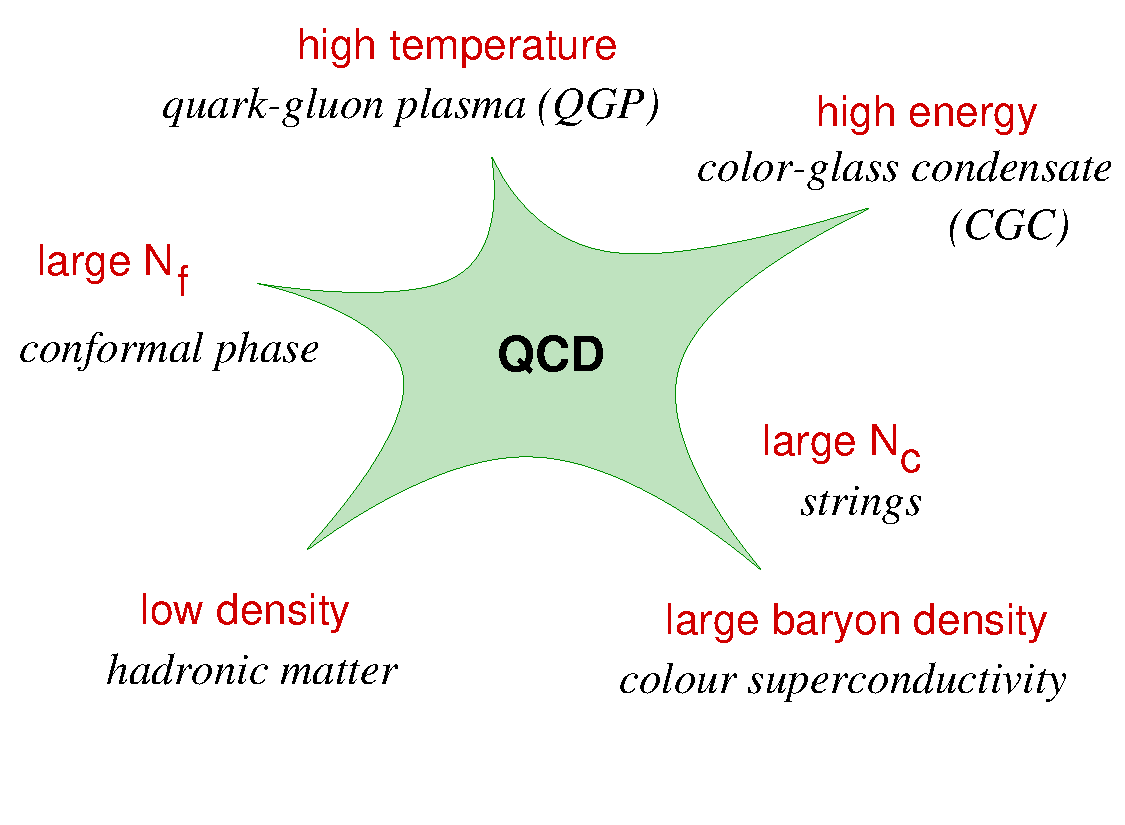
\includegraphics[width=0.6\textwidth]{introduction/schaefer_qcd_phases}
%\vskip -0.7cm
\caption{Many-body dynamics of QCD in different physics limits.}
%\caption{The multiple facets of QCD.}
\label{fig:QCD_facets}
\end{figure}

\subsection*{Deconfinement and chiral symmetry restoration}

Lattice QCD calculations predict a new form of matter at energy densities
(well) above a critical value ---
$\epsilon_c =(6\pm 2) T_c^4 \approx$ 1 GeV/fm$^3$ (Fig.~\ref{fig:latt_EoS}),
where $T_c\approx$ 150--190 MeV is
the critical temperature --- consisting of an extended volume of deconfined and current-mass quarks
and gluons: the Quark-Gluon Plasma (QGP).


\begin{figure}[htb]
\centering
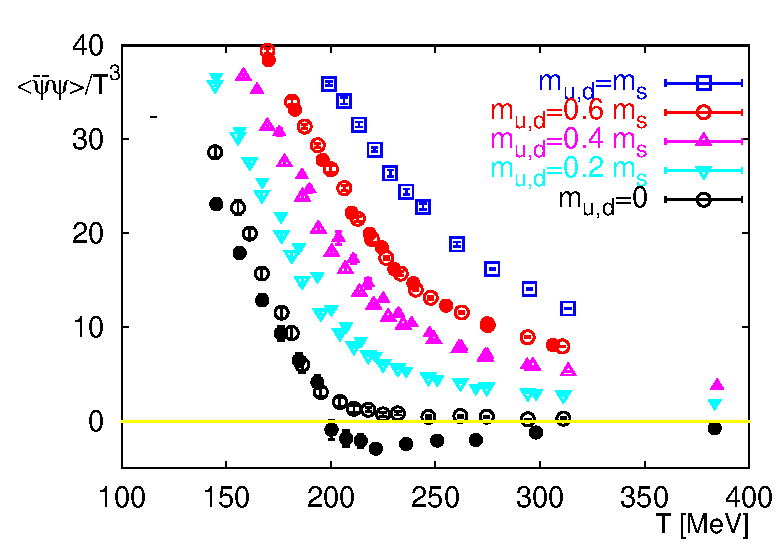
\includegraphics[width=0.48\textwidth]{introduction/latt_qcd_chiral_vs_T}
\includegraphics*[width=0.48\textwidth]{introduction/latt_qcd_EoS}
\caption{Left: The light quark chiral condensate versus the temperature computed in lattice QCD
with various number of flavours and values of the $u,d,s$ quark masses.
Right: The energy density in QCD with 0, 2 and 3 degenerate quark flavours as well as with two light
and one heavier (strange) quarks. %In the case of the SU(3) pure-gauge theory the continuum extrapolated result is shown.
The horizontal arrow shows the value of the Stefan-Boltzmann limit for
an ideal quark-gluon gas}
\label{fig:latt_EoS}
\end{figure}
The vanishing of the chiral condensate at $T_c$ and the sudden liberation of quark and gluon
degrees of freedom are clearly visible in Fig.~\ref{fig:latt_EoS}. The scrutiny of this new state of
matter --- equation-of-state (EoS), order of the phase transition, transport properties, etc. ---
promises to shed light on basic aspects of the strong interaction such as the nature of confinement,
the mechanism of mass generation (chiral symmetry breaking, structure of the QCD vacuum)
and hadronization, which still evade a thorough theoretical description 
due to their highly non-perturbative nature.

In order to calculate physical observables from first principles in QCD it is not enough to
know its Lagrangian. It is also necessary and important to know the true structure of its ground state.
It is just the response of the true QCD vacuum which substantially modifies all the QCD
Green’s functions from their free counterparts.

\subsection*{Parton structure and evolution at small-\texorpdfstring{$x$}{x}}

HERA results indicate that when probed at high energies,
hadrons consist of a very dense system of gluons with small (Bjorken)  momentum
$x=p_{\rm parton}/p_{\rm hadron}$.
At low $x$, the probability to emit an extra gluon is large, proportional to $\alpha_s\ln(1/x)$, and %non-linear
gluon-gluon fusion processes will eventually dominate the parton evolution in the hadronic wavefunctions.
At high virtualities $Q^2$ and moderately low $x$, such evolution %with $Q^2$ (or $\ln(1/x)$)
is described by linear DGLAP or
BFKL equations, suitable for a dilute parton
regime. At $x\lesssim 10^{-2}$, and for $Q$ values below an energy-dependent saturation momentum $Q_s$,
hadrons are however more appropriately
%$Q^2_s \approx\alpha_s\,xG(x,Q^2)/(\pi\,R^2)$, such a configuration
described as dense, saturated parton systems in the context of the ``Colour-Glass Condensate''
(CGC) effective theory with the corresponding non-linear
JIMWLK evolution equations
(Fig.~\ref{fig:CGC_phase_diag}).
%%%Since the growth of the gluon density depends on the transverse size of the hadron,
Low-x gluons in nuclei overlap and, so, saturation effects are expected
to set in earlier for ultrarelativistic heavy nuclei (for which $Q_s^2\propto A^{1/3}$, with $A$
the number of nucleons) than for free nucleons.

\begin{figure}[!Hhtb]
\centering
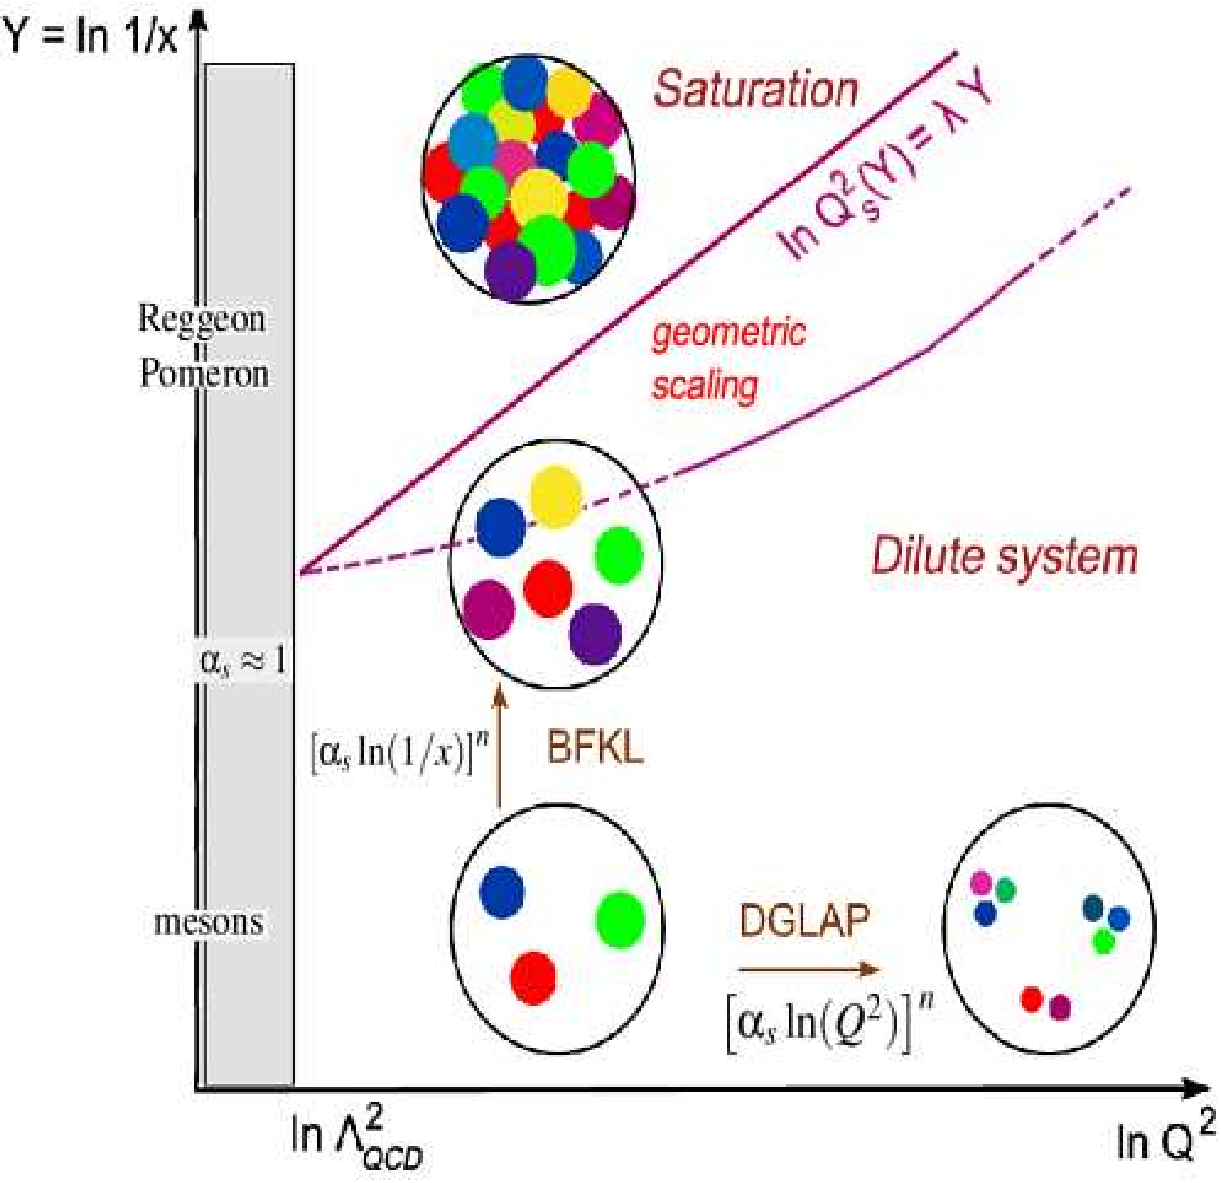
\includegraphics[width=10.cm,height=7.3cm]{introduction/y_Q2_phase_diag_cgc}
\caption{QCD phase diagram in the $1/x,Q^2$ plane (each circle represents a parton with
transverse area $\sim 1/Q^2$ and fraction $x$ of the hadron momentum).  The different evolution
regimes (DGLAP, BFKL, saturation) are indicated, as well as the saturation scale and geometric scaling
curves between the dense and dilute domains}
\label{fig:CGC_phase_diag}
%\vspace{-.4cm}
\end{figure}




\section{Quarkonia}

\end{section}

\end{chapter}









\chapter{Measurments}
The LHC %and CMS -> CMS is emphasized in next sentence allow 
allows for the first detailed studies of the bottomonium family of states in ultra-relativistic heavy-ion collisions.   
Given the momentum resolution attained, and the capability of the trigger system,  CMS is well positioned to lead these studies. 
%
The measurement of bottomonium production and suppression is presented, based on the dataset collected by the CMS experiment during the 2011 PbPb collision run at  $\sqrtsnn = 2.76\TeV$. 


If a deconfined medium is formed in high-energy heavy-ion collisions, one of its most striking expected characteristics is the suppression of quarkonium states~\cite{Matsui:1986dk}. 
This takes place as the force between the constituents of the quarkonium state, a heavy quark and its antiquark, is weakened by the color screening produced by the surrounding light quarks and gluons.
%One of the most triking charateristics associated to quark gluon plasma (QGP) formation  is the suppression of quarkonium states~\cite{Matsui:1986dk}. 
%This is thought to be a direct effect of deconfinement, when the force between the constituents of a quarkonium state, a heavy quark and its antiquark, is weakened by the color screening produced by the surrounding light quarks and gluons.
 The suppression is predicted to occur above a critical temperature of the medium, and sequentially, in the
order of the \QQbar binding energy. 
Since the \PgUa is the most tightly bound state among all quarkonia, it is expected to be the one
with the highest dissociation temperature. % in the QGP.
Such a suppression pattern is expected to further depend on complications arising from additional phenomena sometimes referred to as $hot$ and $cold$ nuclear matter effects~\cite{Brambilla:2010cs,Vogt:2010aa}. 
%
The study of charmonium (\Jpsi, $\psi'$, $\chi_c$) and bottomonium ($\PgUa, \PgUb, \PgUc$, $\chi_b$) production at the unprecedented medium created at the LHC is accordingly much awaited.  
In this note, the measurements of the production and suppression of the $\PgUa$,  $\PgUb$, and  $\PgUc$ states are performed. 

%While all of charmonia as well as excited bottomonia states are expected to be suppressed in the hot and dense medium, the strongly-bound $\PgUa$ state is expected to be the last to melt-down in the QGP.
%
The production of $\PgU$(nS) states is studied by comparing their production rates in PbPb and pp collision data, taken at the same collision energy of $\sqrt{s_{NN}}=2.76\,\TeV$.
In particular, the yield of the higher-mass states is measured relative to the ground state. In this way, we explore the double ratios  --  $\PgU(2S,3S)~vs~\PgUa$ and \PbPb~$vs~\pp$ -- 
which allows a self-calibrating measurement.  
%
Several effects associated to selection, acceptance, and reconstruction mostly cancel, and only remaining factors need to be accounted for,  as corrections to the fitted ratio of raw signal yields.  


Based on the dataset collected during the first LHC PbPb run, at $\sqrtsnn = 2.76\TeV$, in 2010, and in the special $\Pp\Pp$ run at the same energy in early 2011, CMS has published first results on upsilon production and suppression in PbPb collisions. 
%
These included the first evidence for suppression of the excited $\PgU$ states relative to the ground state, at the $2.4\,\sigma$ level~\cite{prl,QM2011}. 
Suppression of the $\PgUa$ state, relative to $\Pp\Pp$ collisions at the same energy, has also been measured~\cite{QM2011,CMS_PAS_HIN-10-006}. 
These two measurements were found to be consistent with suppression of only the excited states, which result in reduced feeddown from excited to ground states. These main results may be summarized as follows:
%
\begin{linenomath}
\begin{eqnarray}
  \PgU(2S+3S)/\PgUa|_{\PbPb} & = & 0.24 _{-0.12}^{+0.13} \pm 0.02\,, \nonumber \\
  \PgU(2S+3S)/\PgUa|_{\pp} & = & 0.78 _{-0.14}^{+0.16} \pm 0.02\,,  \nonumber \\
(\chi \equiv)
  \frac{\PgU(2S+3S)/\PgUa|_{\PbPb}}{\PgU(2S+3S)/\PgUa|_{\pp}}
 & = & 0.31 _{-0.15}^{+0.19} \pm 0.03 \,,  \nonumber \\
(\raa \equiv)
 \frac{\PgUa|_{\PbPb;\, 0-20\%}}{\PgUa|_{\pp}}
& = & 0.681 \pm 0.143 \pm 0.119 \,.  \nonumber
%\label{eq:intro-rat}
\end{eqnarray}
\end{linenomath}

In the 2011 PbPb run, CMS collected a dataset approximately 20 times larger than that gathered in 2010. 
These data will be scrutinized, in order to extract further novel and precision results, during the few years ensuing datataking.
%TBD: note here current LHC PbPb run planning 
In what follows, the corresponding analysis of upsilon suppression is detailed. 


%(online selection, skims, yields)
%\subsection{Minimum bias}
\chapter{Datasets}
\subsection{PbPb dimuon trigger and skim}

A primary dataset (/HIDiMuon/HIRun2011-PromptReco-v1/RECO) based on
all events selected by the muon trigger has been used for this
analysis. The RAW files and the prompt reconstruction files are stored
at T1\_FR\_CCIN2P3. At the Tier-1, they were skimmed for events with
two global muons that form a pair with an invariant mass of more than
2\GeVcc (/HIDiMuon/\\tdahms-Onia2MuMu\_Skim-v3-*/USER). All charge
combinations have been considered in the pairing. In addition to a
muon trigger firing in the event a coincidence with the minimum bias
trigger was required. This minimum bias trigger was defined by the
logical or of the following three triggers, which were unprescaled during the run:
\begin{itemize}
\item A bunch crossing signal sent by the BPTX (BptxAND) and,  two coincident HF
towers above a certain threshold (set in the firmware) on each side of the detector (HcalHfCoincPm) or at least one BSC segment (of the 16) giving a signal on each side of the detector (BscMinBiasThreshold 1):\\
  L1\_HcalHfCoincPmORBscMinBiasThresh1\_BptxAND\_instance1.
\item BSCThreshold1 which requires at least one BSC hit on each side (out of the 32 channels): 'L1\_NotBsc2\_BscMinBiasOR. `NotBsc2' is always 'True' so it can be ignored.
\item coincidence of two HF towers on each side of the detector: HFL1\_HcalHfCoincidencePm.
\end{itemize}

Signal candidates are required to have fired the trigger path  {{HLT\_HIL1DoubleMu0\_HighQ}}. This trigger was unprescaled during the whole run. It is based solely on L1 decisions and requires the
presence of two L1 muon objects with quality $>4$, without any
constraint on their momenta. Coincidence with the BPTX trigger is required. 
The trigger path has tighter quality requirements than the path HLT\_HIL1DoubleMuOpen  
used in the 2010 \PbPb run, and than the path 
HLT\_L1DoubleMu0 used in the 2011 \pp 2.76TeV run. 

Furthermore, the default good event selection as in the 2010 analysis
has been applied. This requires a veto on BSC halo triggers, a
reconstructed primary vertex with two or more tracks, and the pixel
cluster-length being compatible with the primary vertex to reject PKAM
events. An additional requirement to remove UPC (ultra-peripheral collisions) events was the offline
HF coincidence, requiring at least 3 HF towers on each side of the
interaction point with at least 3\GeV energy deposited per tower.

In summary, the events used for this analysis are required to pass the
following filters : the BSC halo filter, a reconstructed primary
vertex made of at least two tracks, the pixel cluster-length
compatibility with the vertex, the requirement of an off-line HF
coincidence with at least 3 towers on each side of the interaction
point in the HF with at least 3 GeV energy deposited per tower, and the  {{HLT\_HIL1DoubleMu0\_HighQ}} muon trigger.

The CMSSW release 4\_4\_2\_patch5 and the global tag GR\_P\_V27A were
used during the skimming and analysis steps.

\subsection{pp sample}

The same \pp sample as for the 2010 analysis has been used~\cite{CMS_PAS_HIN-10-006,prl,QM2011}. 
Signal candidates are required to have fired the trigger path HLT\_L1DoubleMu0.
%{{HLT\_HIL1DoubleMuOpen}} => this pone was used for pbpb data in 2010
%
The data have been re-reconstructed in the same CMSSW release as the 2011 \PbPb
data (4\_4\_2\_patch5) with the global tag GR\_R\_44\_V10:
/AllPhysics2760/Nov2011\_HI-SD\_MuHI-276TeV\_ppRereco/RECO.

%summary of path names:
%PbPb (old MC): HLT_HIL1DoubleMuOpen_v1
%PbPb (new MC): HLT_HIL1DoubleMu0_HighQ_v1
%pp (old MC): HLT_L1DoubleMu0_v1
%pp (newd MC): HLT_HIL1DoubleMu0_HighQ_v1


\subsection{Monte Carlo samples}

\PgUa events were simulated in \PYTHIA and embedded into
\textsc{hydjet} as for last year's analysis. For this \PgUa were
generated with realistic \pt and rapidity distributions in several
bins of \pt (0--3, 3--6, 6--9, 9--12, 12--15, 15--30, and $>30\GeVc$)
to enhance the statistics at high \pt:\\
/Hydjet\_Bass\_MinBias\_2760GeV/davidlw-PyquenEvtGen\_upsilon1sMuMu\_upsPt*-Summer11-STARTHI44\_V7-v1-GEN-SIM-RECO\_v3-58956c214fa8e92cbba029d2c88707a9/USER

\end{chapter}


\chapter{Fitting}
The parameters of interest are extracted from the data samples via an extended unbinned maximum likelihood fit to the dimuon invariant-mass spectra.
In this section, the fitter study is carried out for two selected $p_{T}^{\mu}$ cut, 3.5 and 4.0 $\GeVc$. 
But the final results in Section~\ref{sec:dooubleratio} is given with the nominal 4.0 $\GeVc$ cut only. 
The baseline fitting model is improved relative to the publication using the 2010 dataset. We explored complementary approaches for background modeling (eg employing like-sign parameterizations, track rotation).
%

The baseline fitting model is inspired in that used in~\cite{CMS_AN_2010-140, CMS_AN_2011_062}. 
%
Each of the $\PgU$(nS) signals is modeled via a crystal-ball shape (CB), 
which consists of a Gaussian function with the low-side tail replaced with a power law describing final-state radiation (FSR). 
%
The crystal-ball function is given by:
%
\begin{linenomath}
\begin{equation}
  f(x;\alpha,n,\bar x,\sigma) = N \cdot \left\{
  \begin{array}{ll}
    \exp(- \frac{(x -\bar x)^2}{2 \sigma^2})      & \mbox{for } \frac{x - \bar x}{\sigma} > -\alpha \\ 
    A \cdot (B - \frac{x - \bar x}{\sigma})^{-n}  & \mbox{for } \frac{x - \bar x}{\sigma} \leq -\alpha \,,
  \end{array} 
  \right.
\end{equation}
\end{linenomath}
%
where 
\begin{linenomath}
\begin{eqnarray}
  A & = & \left(\frac{n}{\left| \alpha \right|}\right)^n \cdot \exp\left(- \frac {\left| \alpha \right|^2}{2}\right) \,, \nonumber \\
  B & = & \frac{n}{\left| \alpha \right|} - \left| \alpha \right| \,. \nonumber
\end{eqnarray}
\end{linenomath}
%
The CB function is parameterized by four parameters -- the mass mean $\bar x$ and resolution $\sigma$, and the tail parameters $\alpha$ and $n$ -- which are constrained amongst the three signal peaks:    
the tail parameters are common; 
the resolution  forced to scale with the resonance mass;  
the differences of the mass means are fixed to their PDG values. % ($\Delta_{12}=563\MeVcc$, $\Delta_{13}=332\MeVcc$). 

%The floating fit parameters are the resonance yield and/or yield-ratios, the $\PgUa$ mass, and all of the background parameters. The fits to the pp and PbPb data are shown in \fig{fig:ups_pp_and_PbPb_separate} 

In the previous iteration of the analysis~\cite{prl}, based on the 2010 dataset, 
the signal PDF shape parameters were fixed from MC simulation: $\alpha=1.6$, $n=2.3$, $\sigma_{1S}=92\MeVcc$. 
%
In view of the larger dataset currently available, such constraints have been relaxed. %, based on the studies documented next.  
Specifically, the following signal shape parameters are free in the fit:
the $\PgUa$ mass mean and resolution, the tail parameter $\alpha$.
Note that, given $\alpha$ and $n$ are strongly correlated, the constraint $n=2.3$ is kept in the fit. 


The $\pt$ threshold applied for muon selection induces a sculpting of the mass background distribution, as described in Section~\ref{sec:shoulder}.  
%\emph{(add reference to the relevant section in the selection chapter)}. 
The background parameterization adopted corresponds to an exponential function (exp), multiplied by an error-function (erf), where the latter describes the induced kinematic shoulder and is defined as:
%
\begin{linenomath}
\begin{equation}
\mbox{erf}(x)=\frac{2}{\sqrt{\pi}}\int_0^x e^{-t^2} \: dt
\end{equation}
\end{linenomath}
%
The background model is thus described by three parameters: the exponential decay constant, and the turn-on mean and width. All background parameters are left free. % for the nominal $\pt>3.5 \GeVc$ selection. 
%For the  $\pt>4.0 \GeVc$ case, the shoulder is located within the signal region, and the error-function parameters need to be constrained -- in this case, the background peaks under the signal peak, and the fit cannot reliably descriminate signal from background for events under the CB tail. 

The nominal fit results to the PbPb data are shown in \fig{fig:massfit_nominal_all}. 
%
% https://espace.cern.ch/cms-heavyion/upsilon/fitting/errorFunction_70microb.aspx
%
\begin{figure}[hbtp]
  \begin{center}
    \subfigure[$\pt^\mu>3.5\GeVc$]{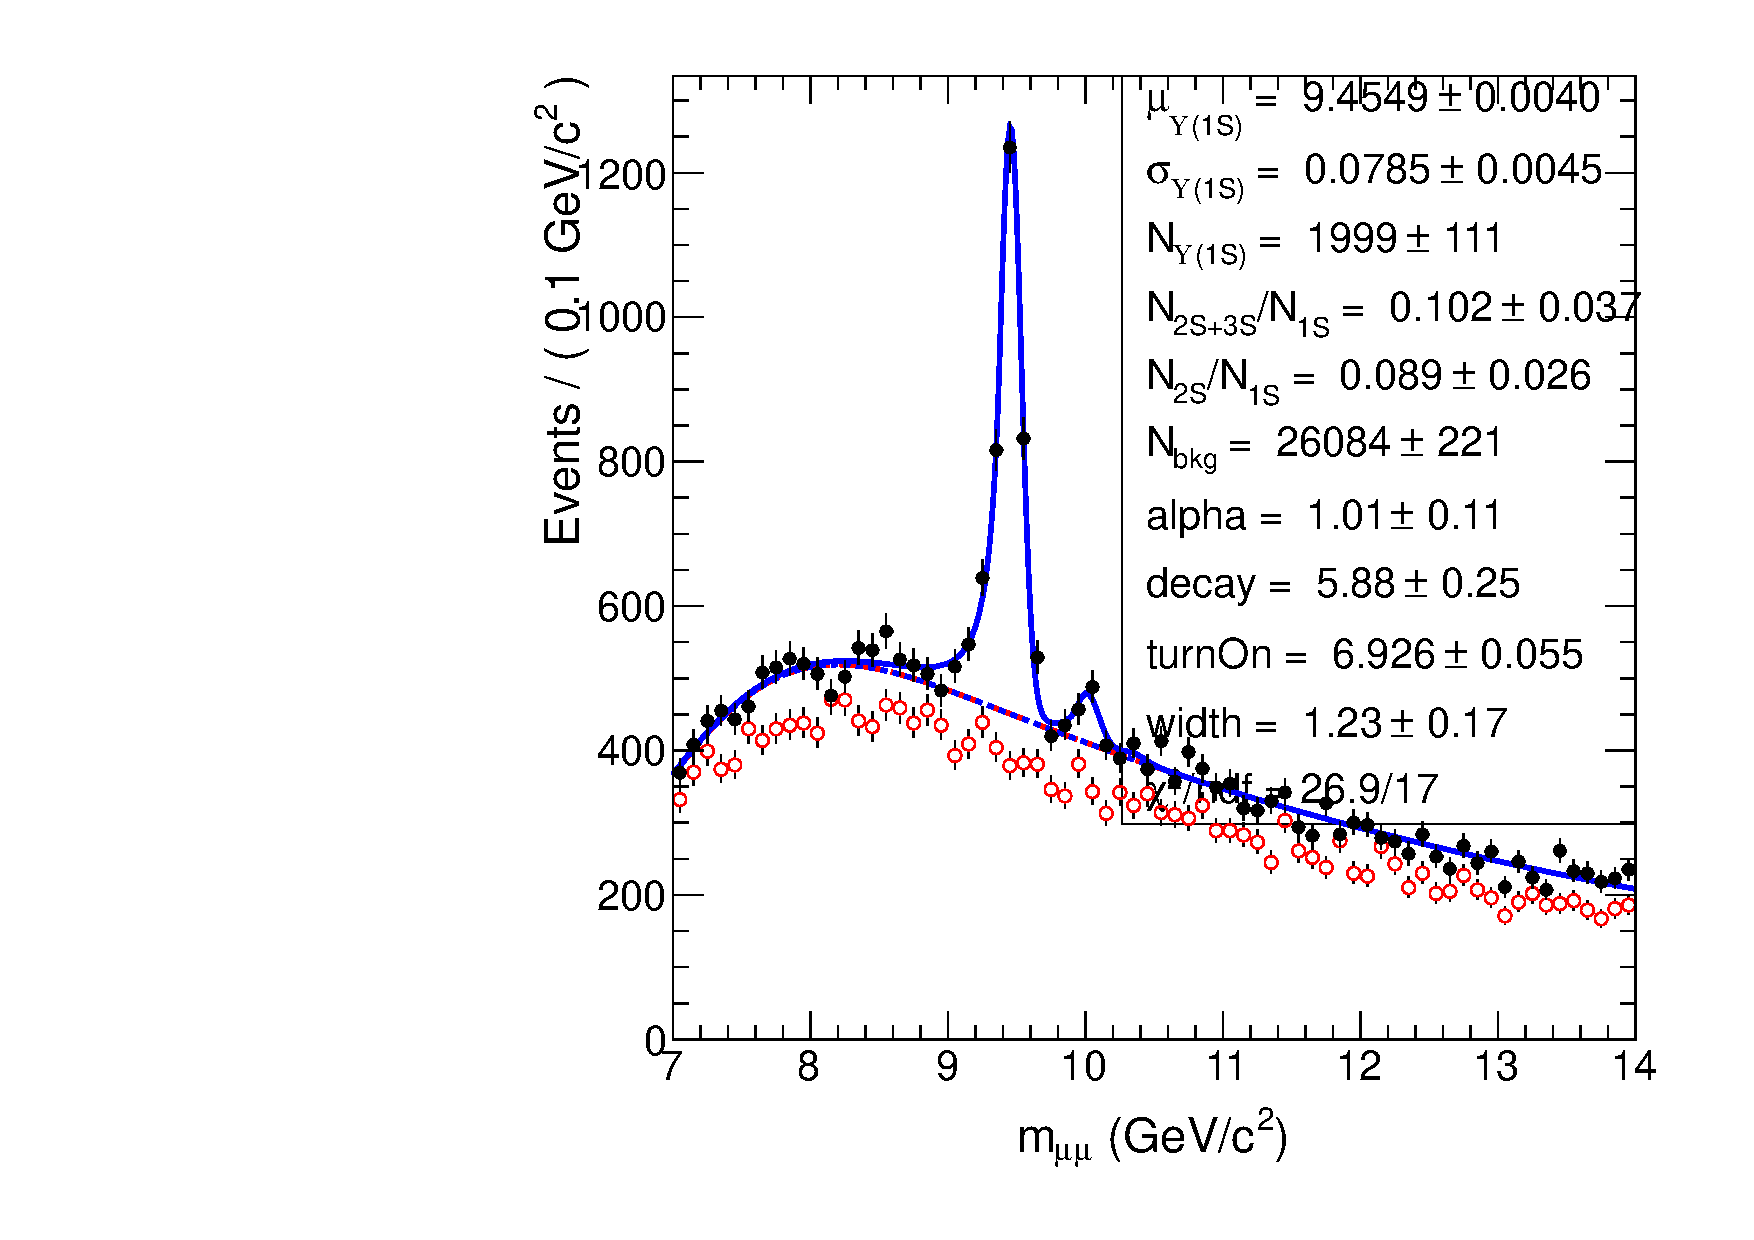
\includegraphics[angle=0,width=0.5\textwidth]{figures/fitting/masspeak_Hi_paramOn_MuonPT35_150imub}}
    \subfigure[$\pt^\mu>4.0\GeVc$]{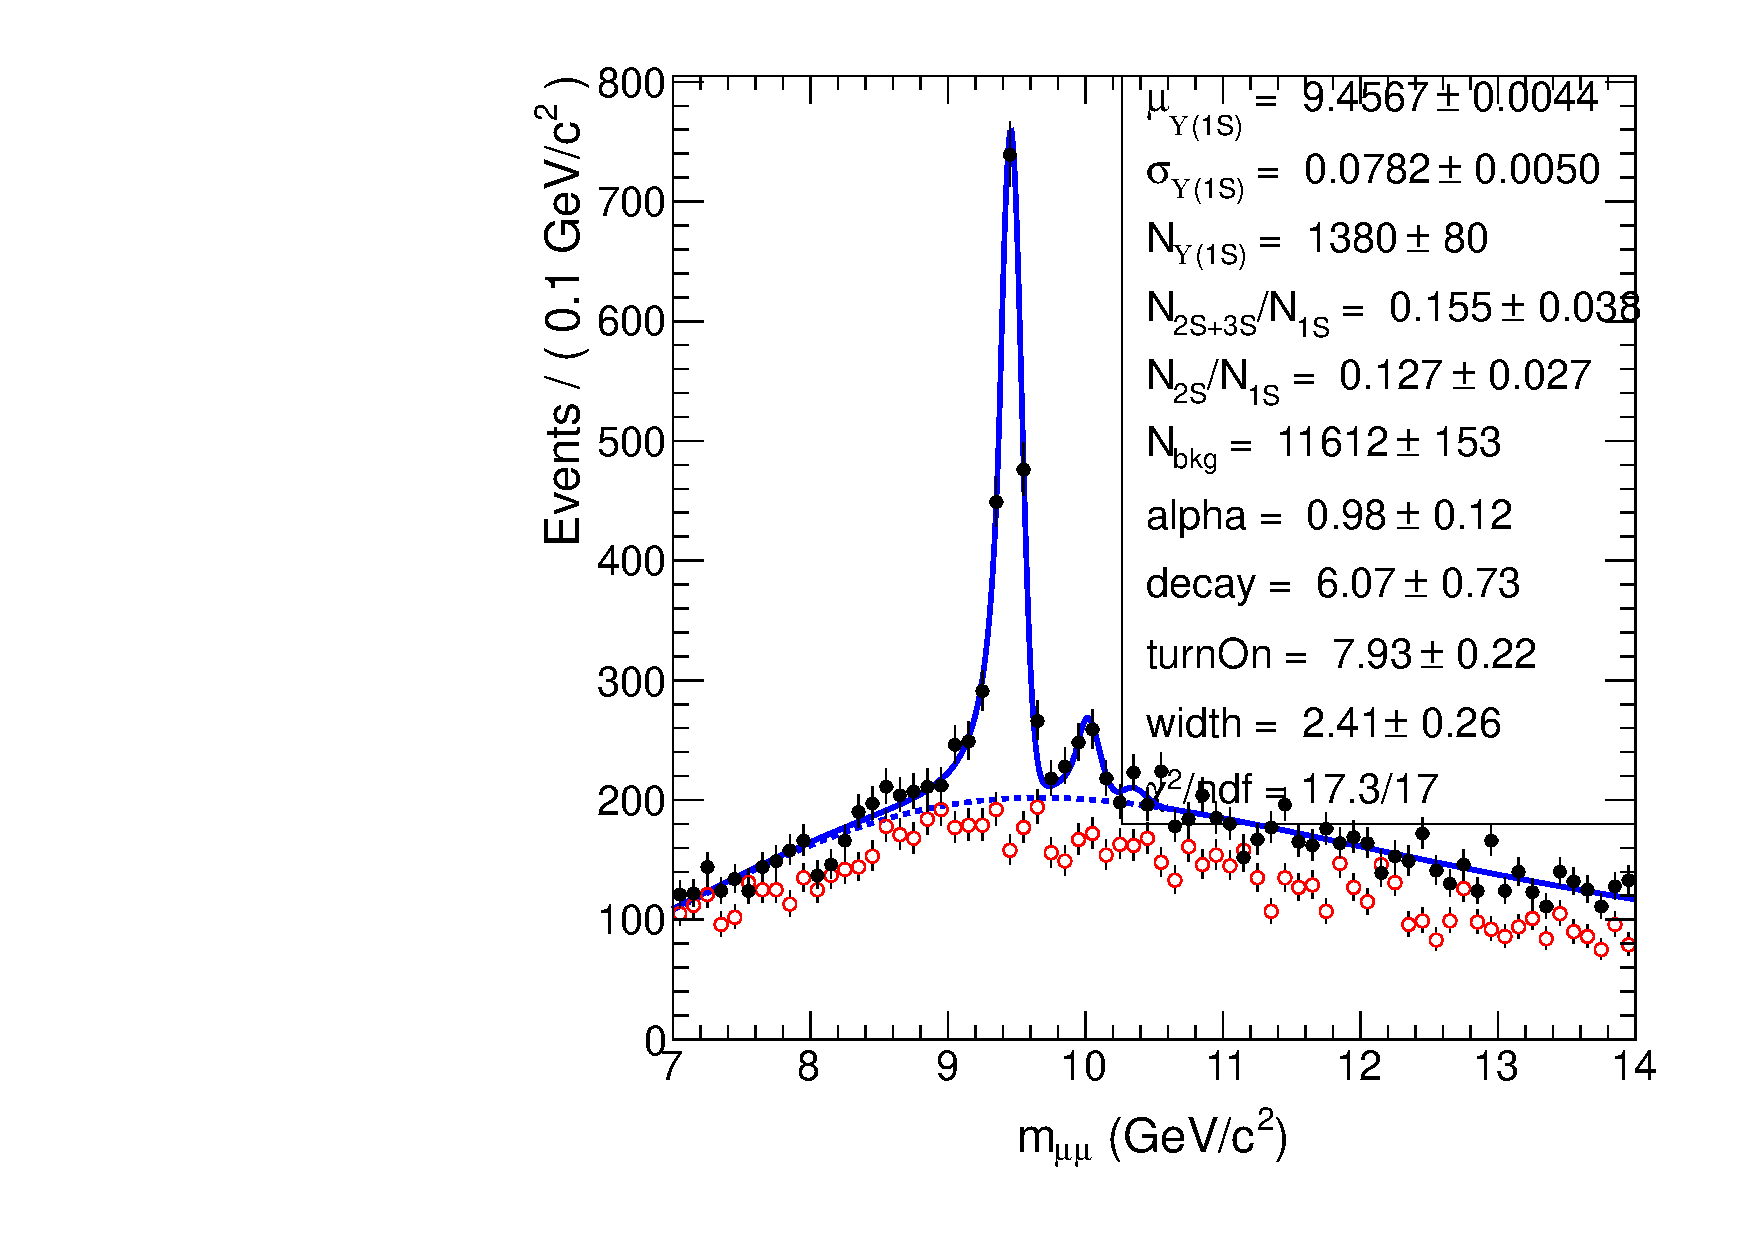
\includegraphics[angle=0,width=0.5\textwidth]{figures/fitting/masspeak_Hi_paramOn_MuonPT4_150imub}}\label{fig:massfit_nominal}
  \caption{Fit to the dimuon invariant-mass distributions, for the PbPb sample. ($150 \mu b^{-1}$) }
  \label{fig:massfit_nominal_all}
  \end{center}
\end{figure}

\subsection{Signal model studies}


\subsubsection{Final state radiation model}

% https://espace.cern.ch/cms-heavyion/upsilon/fitting/RadiationTailFromMC.aspx

We first estimate the CB tail from Monte Carlo simulation of final state radiation. % (enter reference for Photos / EvtGen interface to Pythia). 
The MC sample is first split in multiple (about 50) sub-samples, of statistics comparable to data. These samples are fitted in turn, and the average parameter values are determined. This is shown in~\fig{fig:fsr_mc_pull}. 
%The values obtained are ... No!: let;s avoid having too many numbers spread in the text, which we will not be able to "maintain" -- instead summarize numbers in tables only
 
\begin{figure}[hbtp]
  \begin{center}
    \subfigure[fixed: $\sigma = 92 \MeVcc$, $n=2.3$; float: $\alpha$  ]{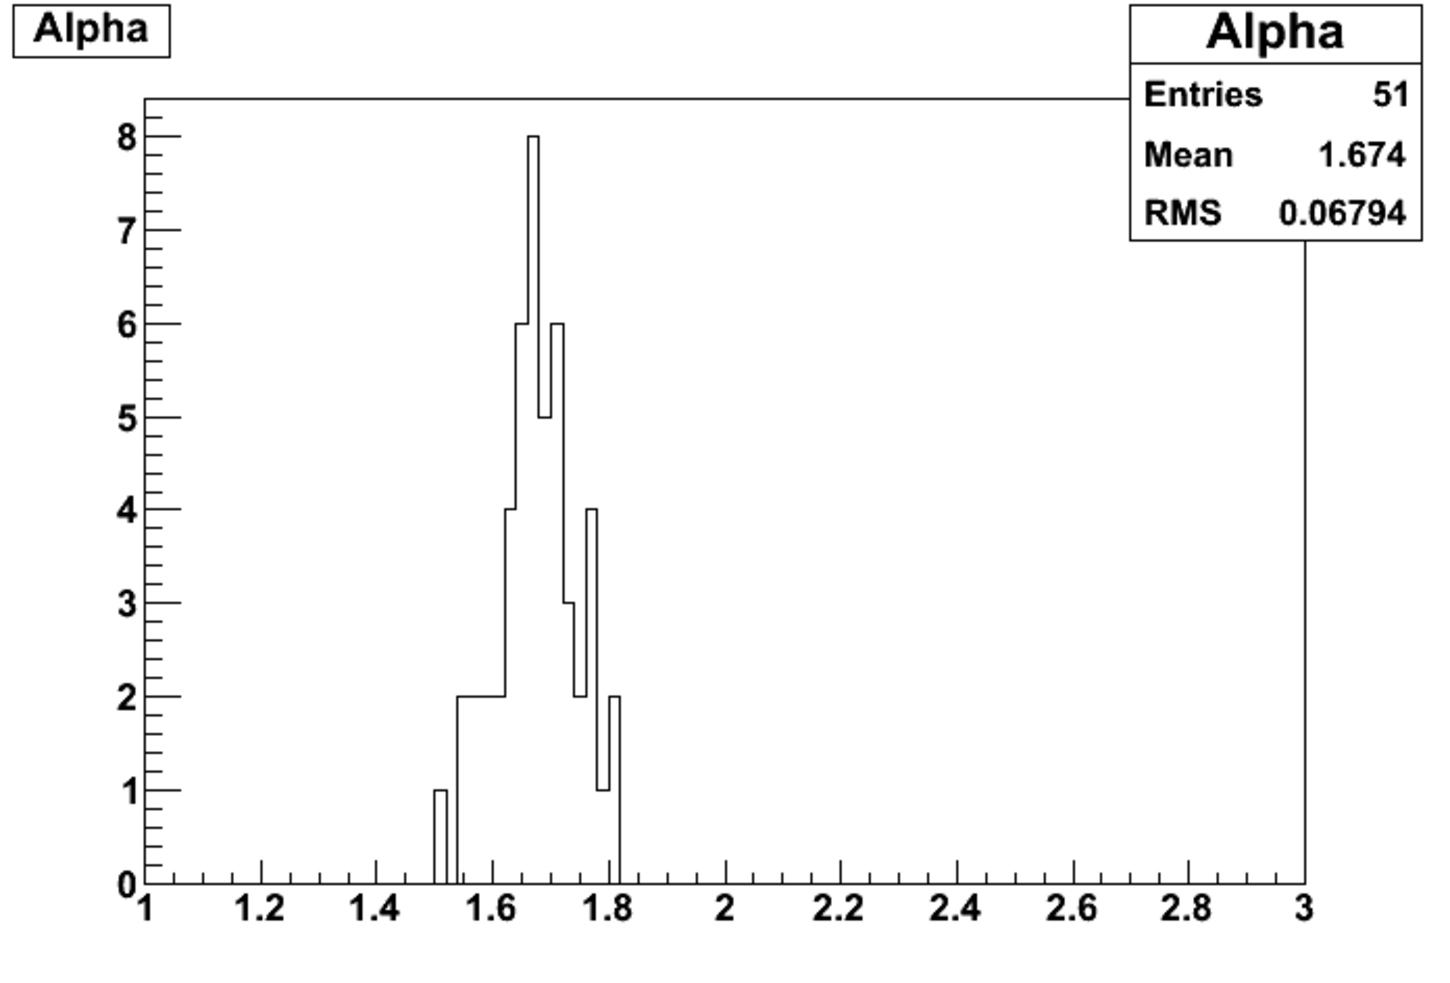
\includegraphics[angle=0,width=0.5\textwidth]{figures/fitting/mc_fsr_mean_alpha.pdf}}
    \subfigure[fixed: $\sigma = 92 \MeVcc$, $\alpha=1.674$; float: $n$]{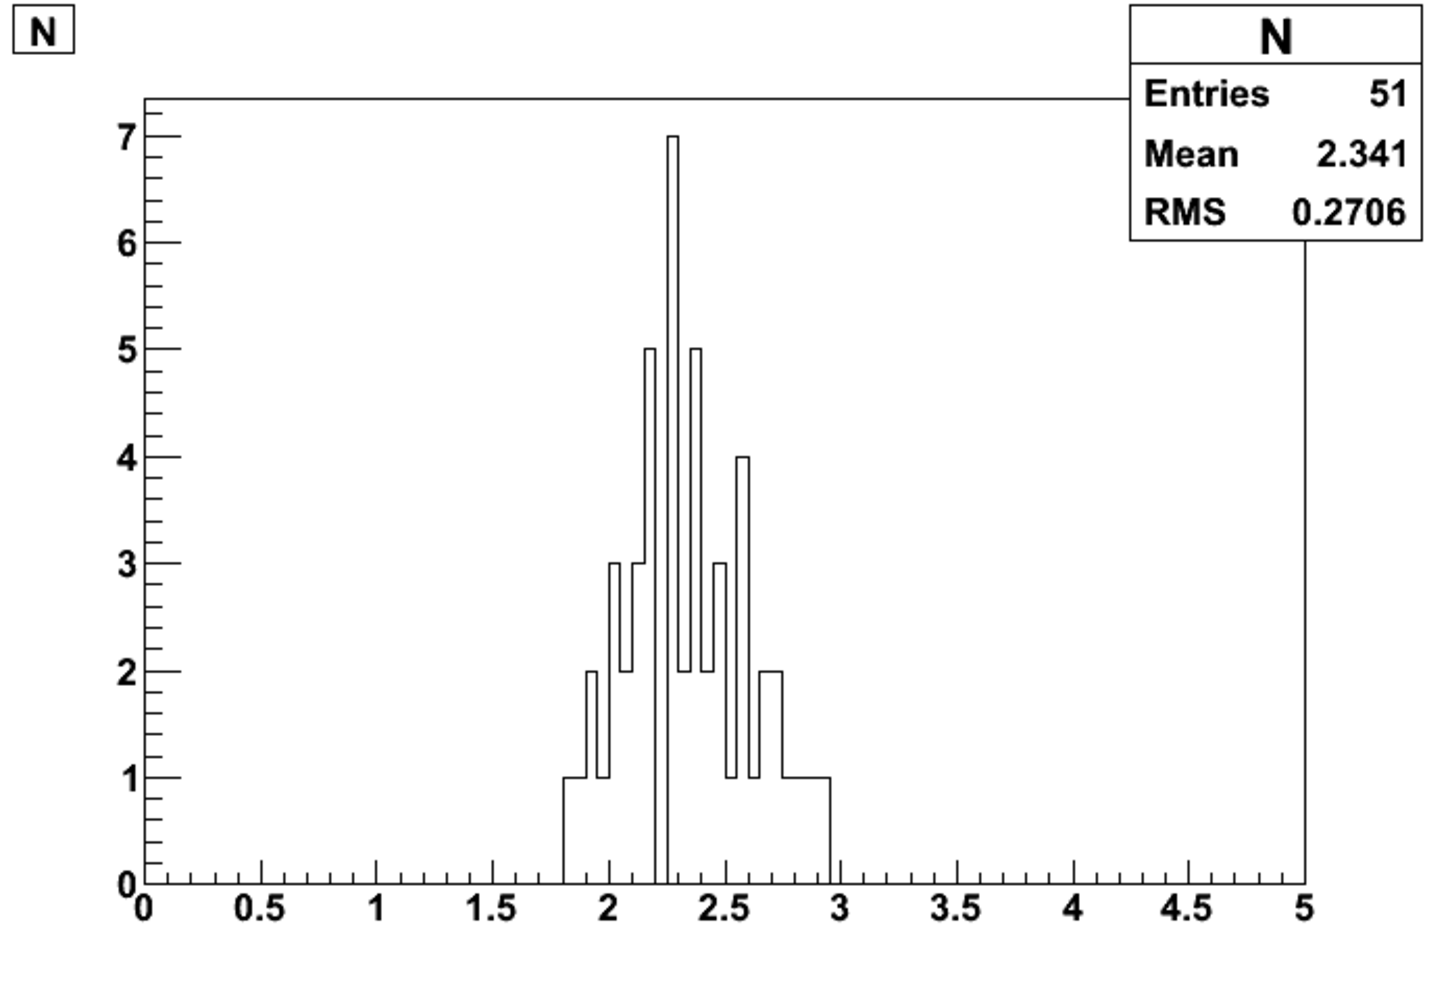
\includegraphics[angle=0,width=0.5\textwidth]{figures/fitting/mc_fsr_mean_n.pdf}}
  \caption{FSR parameter estimation from MC.}
  \label{fig:fsr_mc_pull}
  \end{center}
\end{figure}

For estimating the CB tail from data, the fit is performed after subtracting the  like-sign dimuon mass distribution. This procedure results in a mostly flat remaining background. In this way, the (binned) fit to the subtracted data is able to better constrain the background shape from the mass side-bands, allowing also a more reliable determination of the CB tail. Fit examples are shown in~\fig{fig:fsr_data_bins}. 


\begin{figure}[hbtp]
  \begin{center}
    \subfigure[bins:100]{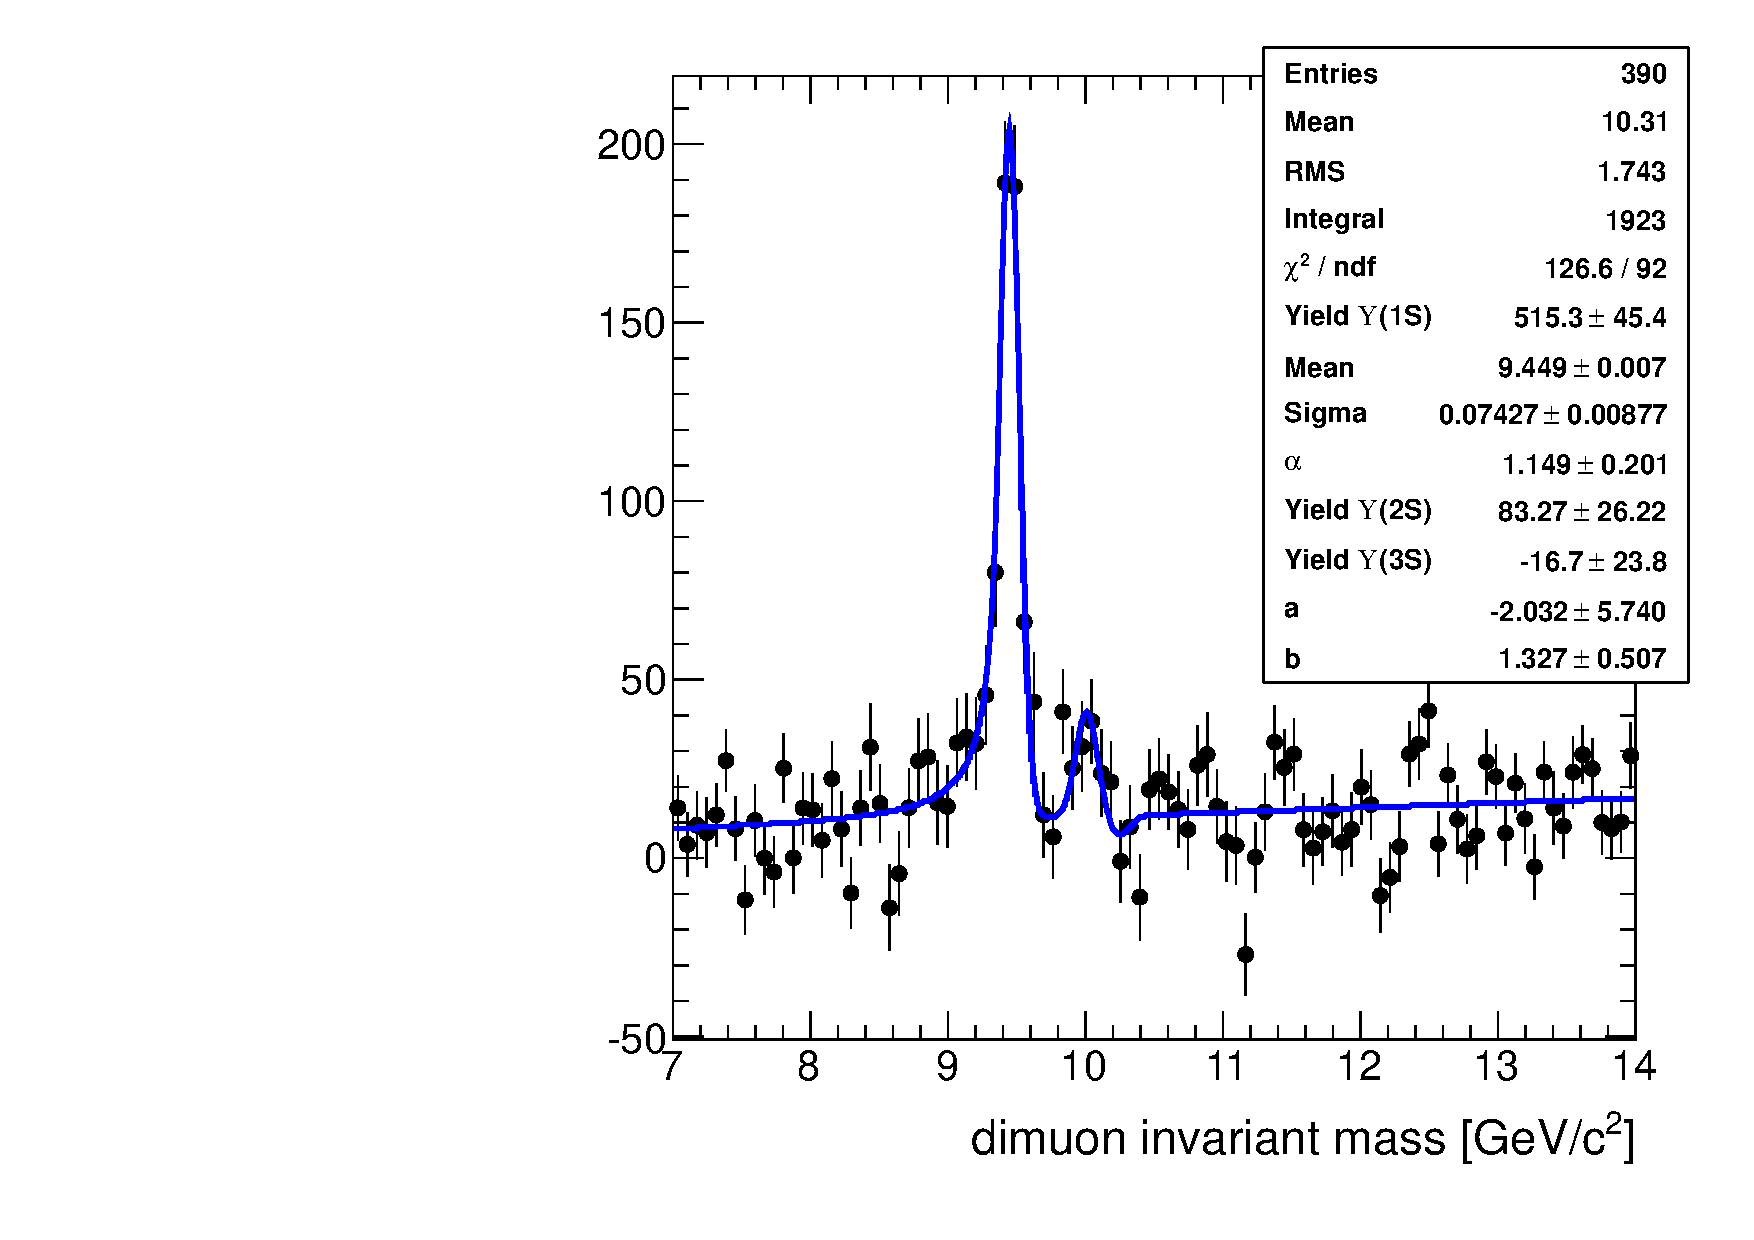
\includegraphics[angle=0,width=0.3\textwidth]{figures/fitting/fit_subtract_1stOrder_fixn_100bin.pdf}}
    \subfigure[bins:70]{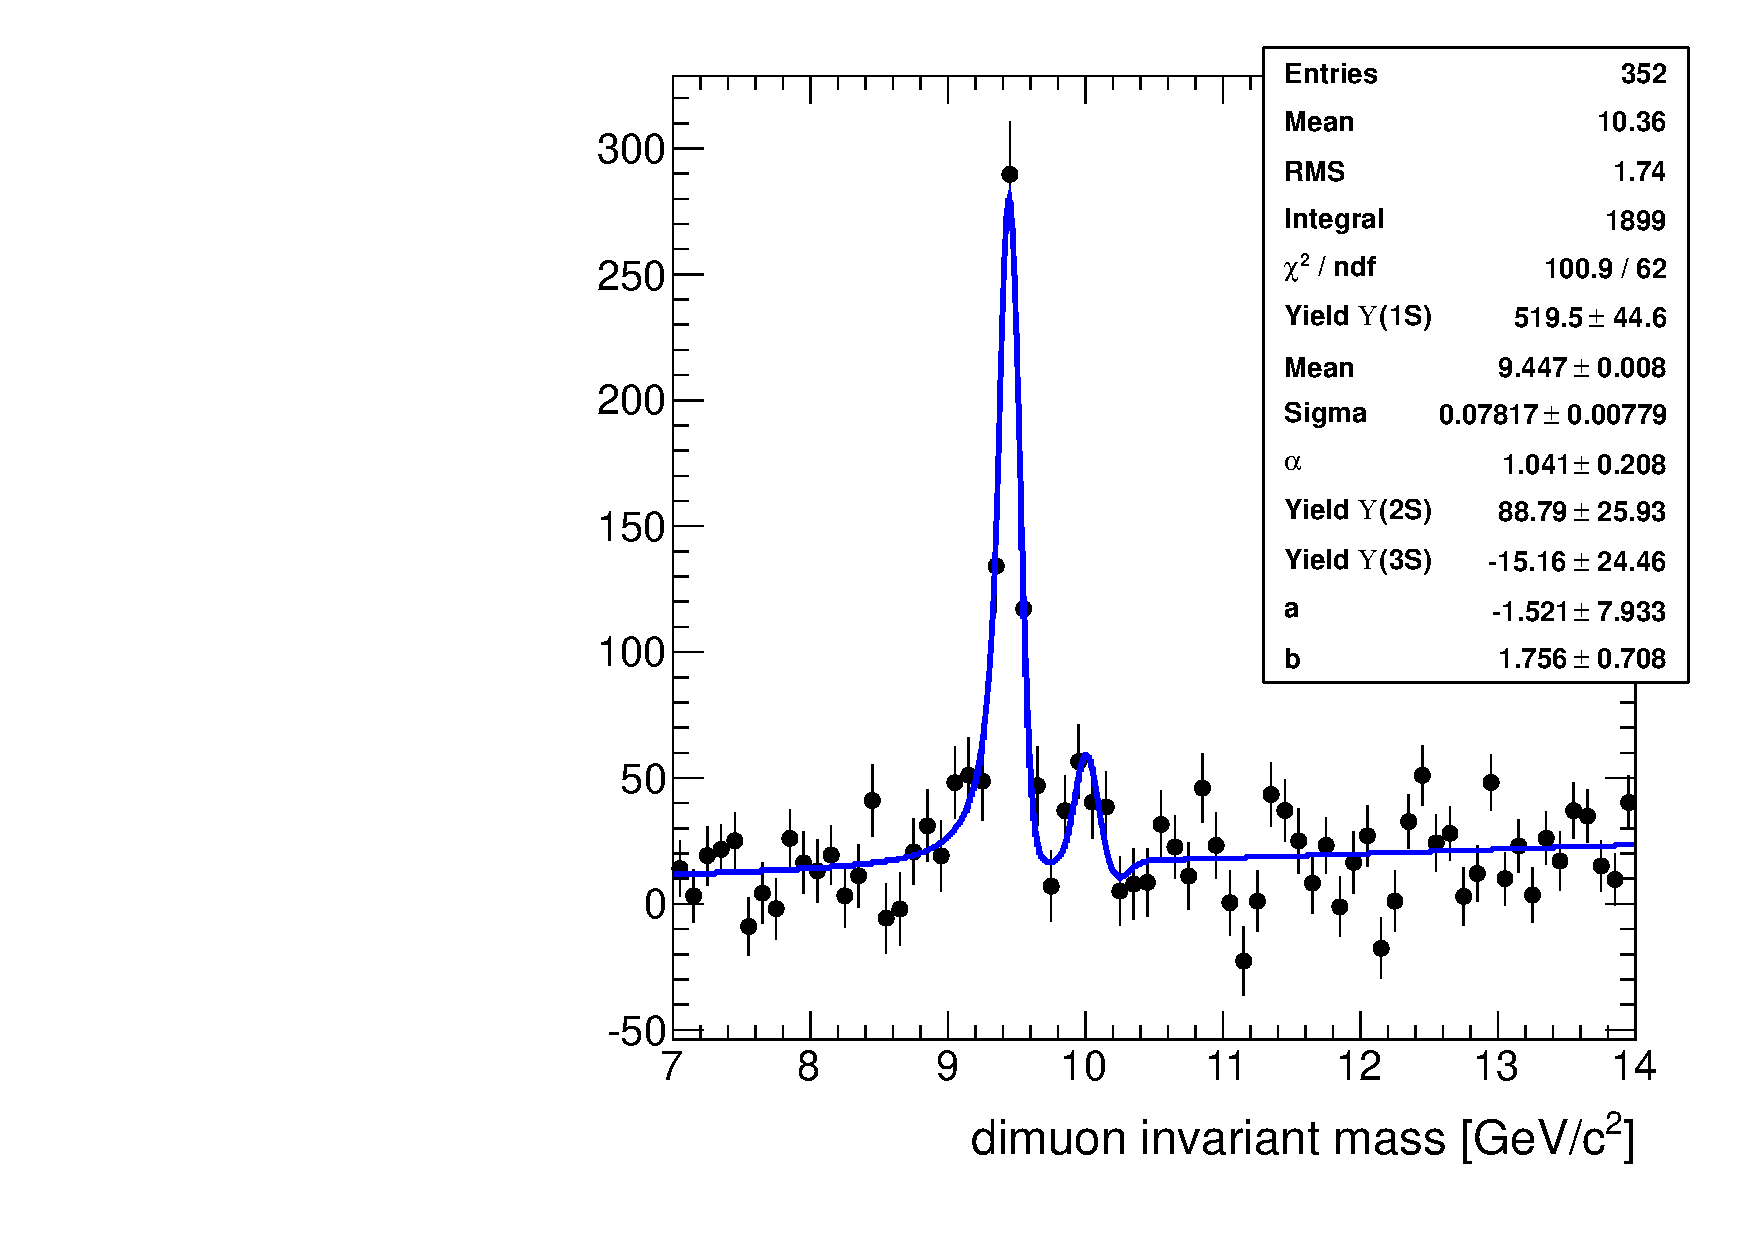
\includegraphics[angle=0,width=0.3\textwidth]{figures/fitting/fit_subtract_1stOrder_fixn_70bin.pdf}}
    \subfigure[bins:50]{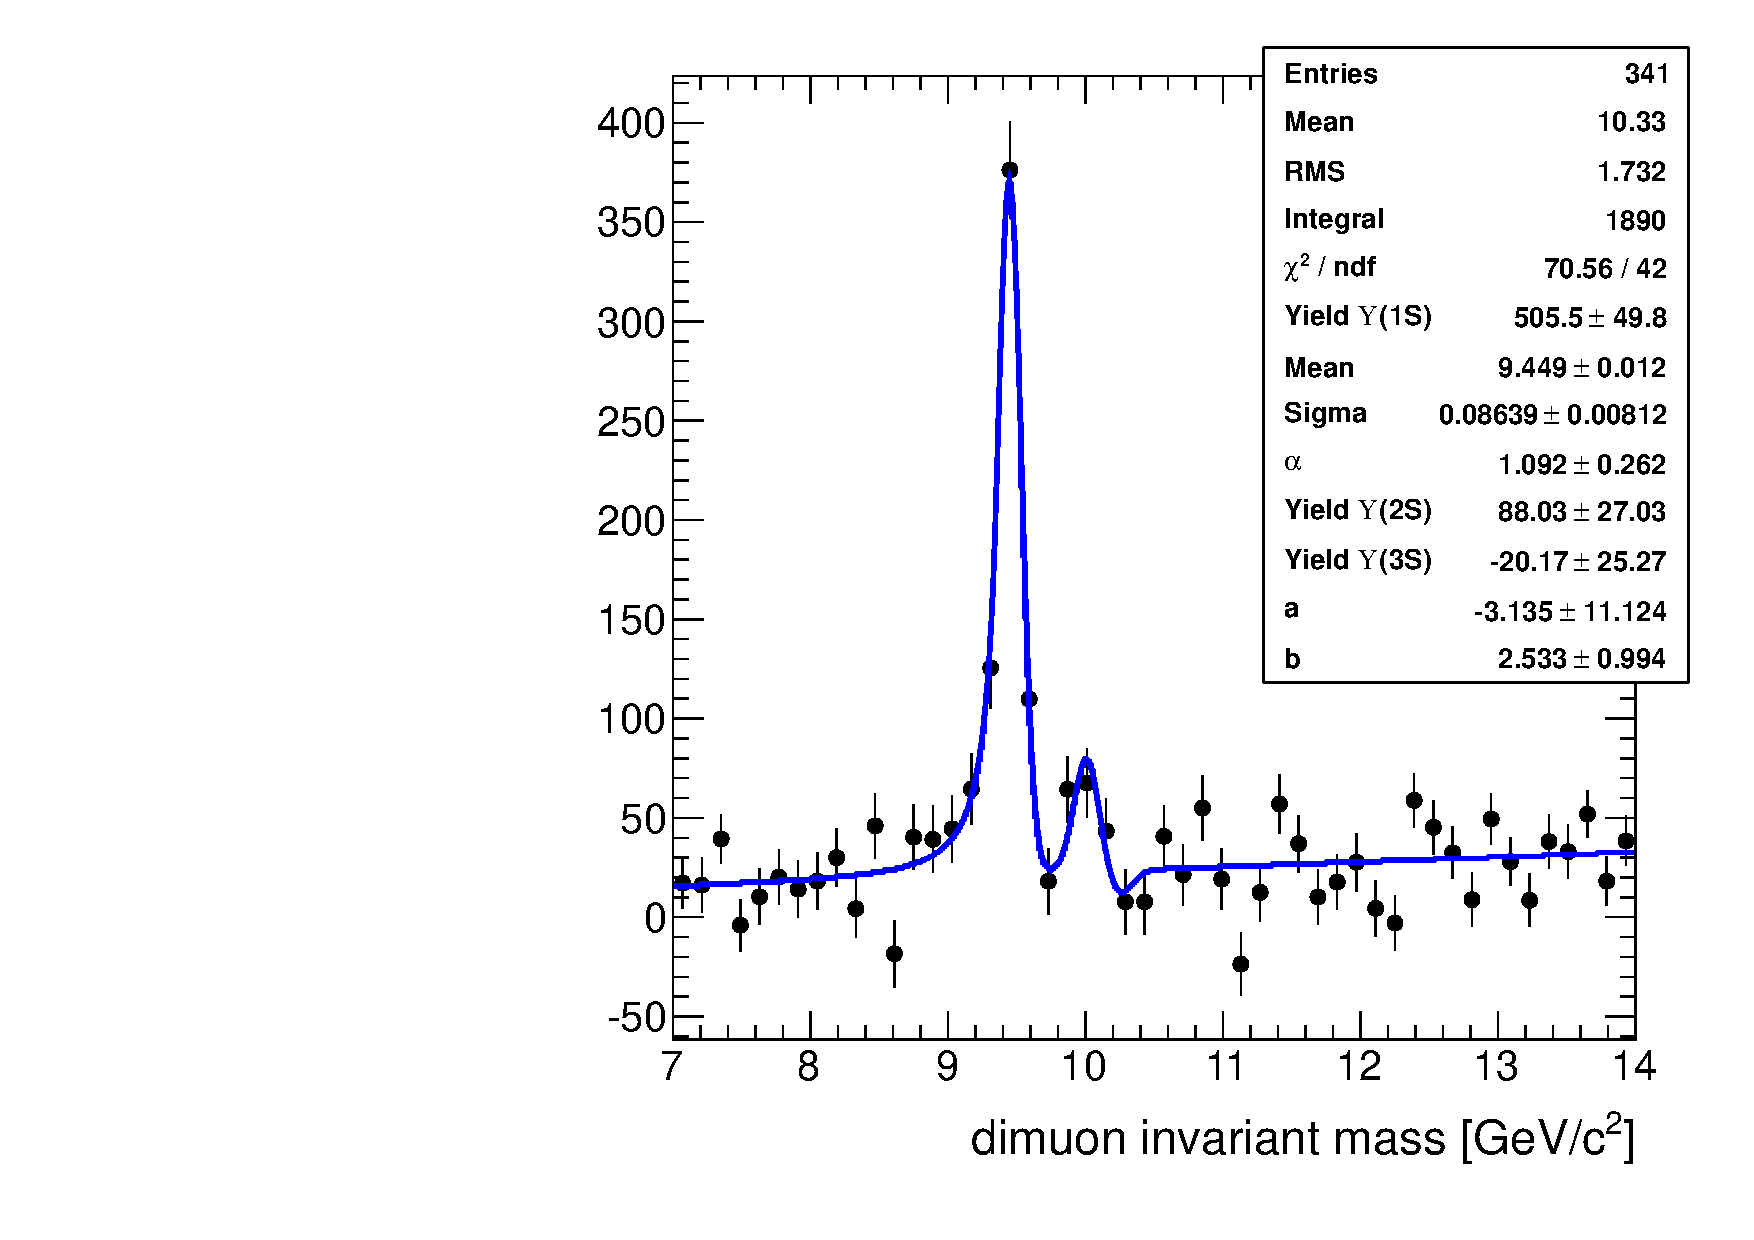
\includegraphics[angle=0,width=0.3\textwidth]{figures/fitting/fit_subtract_1stOrder_fixn_50bin.pdf}}
  \caption{FSR parameter estimation from like-sign subtracted data.}
  \label{fig:fsr_data_bins}
  \end{center}
\end{figure}



Table~\ref{tab:fsr} summarizes the CB tail parameter estimations achieved from simulation and data. 
%
It illustrates the level of variations that may be attained. 
In the nominal configuration, the $\alpha$ CB parameter is determined from the fit to the data. 
%
\begin{table}[!h]
  \centering
  \caption{Final state radiation and resolution parameter values.}
  \begin{tabular}{c|c c c}
    \hline
    & $\alpha$ & $n$ (fixed) & $\sigma \; (\MeVcc)$ \\
    \hline
    Monte Carlo   & $1.67 $ & 2.3  & $90$ \\
    \pp 7 TeV data  & $1.4 \pm 0.1$ & 2.3  & $62 \pm 2$ \\
    like-sign subtracted \PbPb data & $1.0 \pm  0.3$ & 2.3 & $73 - 87$ \\ %TBD: needs to re-done withh corercted data!!
    \PbPb data (nominal fit) & $0.98 \pm 0.2 $ & 2.3  & $78.2 \pm 0.5$ \\
    \PbPb and \pp data (nominal simul. fit) & $1.12 \pm 0.13 $ & 2.3 & $79.4 \pm 0.4$\\
    \hline
  \end{tabular}
  \label{tab:fsr}
\end{table}
%https://espace.cern.ch/cms-heavyion/upsilon/fitting/fsr_pp_study.aspx
%https://espace.cern.ch/cms-heavyion/upsilon/fitting/likesign_181912-182609.aspx
%https://espace.cern.ch/cms-heavyion/upsilon/fitting/RadiationTailFromMC.aspx

%\FloatBarrier

\subsection{Background model studies}
\label{sec:bgmodel}

%Previosuly~\cite{prl}, the background has been described by a second-order polynominal in the mass-fitting range $7-14\GeVcc$. 
%In view of the increased statistics, a more detailed treatment is now pursued, as documented in the following sections. 

We explore alternative estimations and parameterizations of the background, with respect to the second order polynomial model used in~\cite{CMS_AN_2010-140, CMS_AN_2011_062}.  

\subsubsection{Like-sign dimuon spectrum}
\label{sec:like-sign}

Here we carry out fits to the upsilon data, by constraining the background model utilizing information from the like-sign dimuon spectrum. 
The like-sign dimuon combinations contain no signal component, and provide a useful handle to estimate the combinatorial background shape in the mass region under the signal peaks. 
The like-sign spectrum is not expected to match \emph{exactly}, in shape and normalization, the combinatorial opposite-side spectrum: 
different, small contributions may arise from Drell-Yan and open flavor sources. This residual component is expected to be smooth and non-peaking, and is accommodated by allowing an extra polynomial component in the fit the (oppositely charged dimuon) data. 

The like-sign dimuon mass distribution is employed to define a PDF component, in the following two ways: 
\begin{itemize} 
\item {\bf{Like-sign dataset smoothing.}} 
We use the RooFit implementation via the class RooKeysPdf~\cite{rookeyspdf}, which implements a one-dimensional kernel estimation PDF which models (smoothens) the distribution %of an arbitrary input dataset 
as a superposition of Gaussian kernels, one for each data point, each contributing 1/N to the total integral of the PDF.  
%\emph{(add reference: Cranmer KS, Kernel Estimation in High-Energy Physics. Computer Physics Communications 136:198-207,2001 - e-Print Archive: hep ex/0011057)} 

\item {\bf{Like-sign parameterized fit.}} 
We fit the like-sign distribution utilizing an $\text{Erf} \times \text{Exp}$ model. 
The high-mass spectrum is well described by an exponential,  
%We motivate the exponential to account 
describing random track combinations. 
To describe the acceptance turn-on shape induced by the single muon kinematic threshold, 
 %below the $\PgU$ peak ????
the exponential is multiplied by an error function. 
%an error-function is multiplied to the .
 %like-sign combinations at higher mass. 
%For $\pt>3.5 \GeVc$ the parameters are $m0shift$ $6.910 \pm 0.073 \GeVcc$ and $width$ $1.18 \pm 0.21 \GeVcc$. 
Tested variations of the turn-on function parameters gave negligible deviations of the extracted yields. 
\end{itemize} 

The shape of the like-sign distribution matches well that of the mass sidebands in the opposite-sign sample. 
The fit to the opposite-sign signal sample is performed employing a linear combination of the like-sign extracted PDF,  along with an extra polynomial component. The latter is included in order to allow for potential discrepancies that might arise between the like-sign and opposite-sign mass spectra.
The fit results are displayed in~\fig{fig:massfits_likesign} 
%(and in~\fig{fig:massfits_likesign_35} fot the 3.5 \GeVc cut instead of the nominal 4.0), 
and demonstrate a good description of the data. 


\begin{figure}[hbtp]
  \begin{center}
    \subfigure[$\pt^\mu>3.5\GeVc$, rookeyspdf, $70 \mu b^{-1}$]{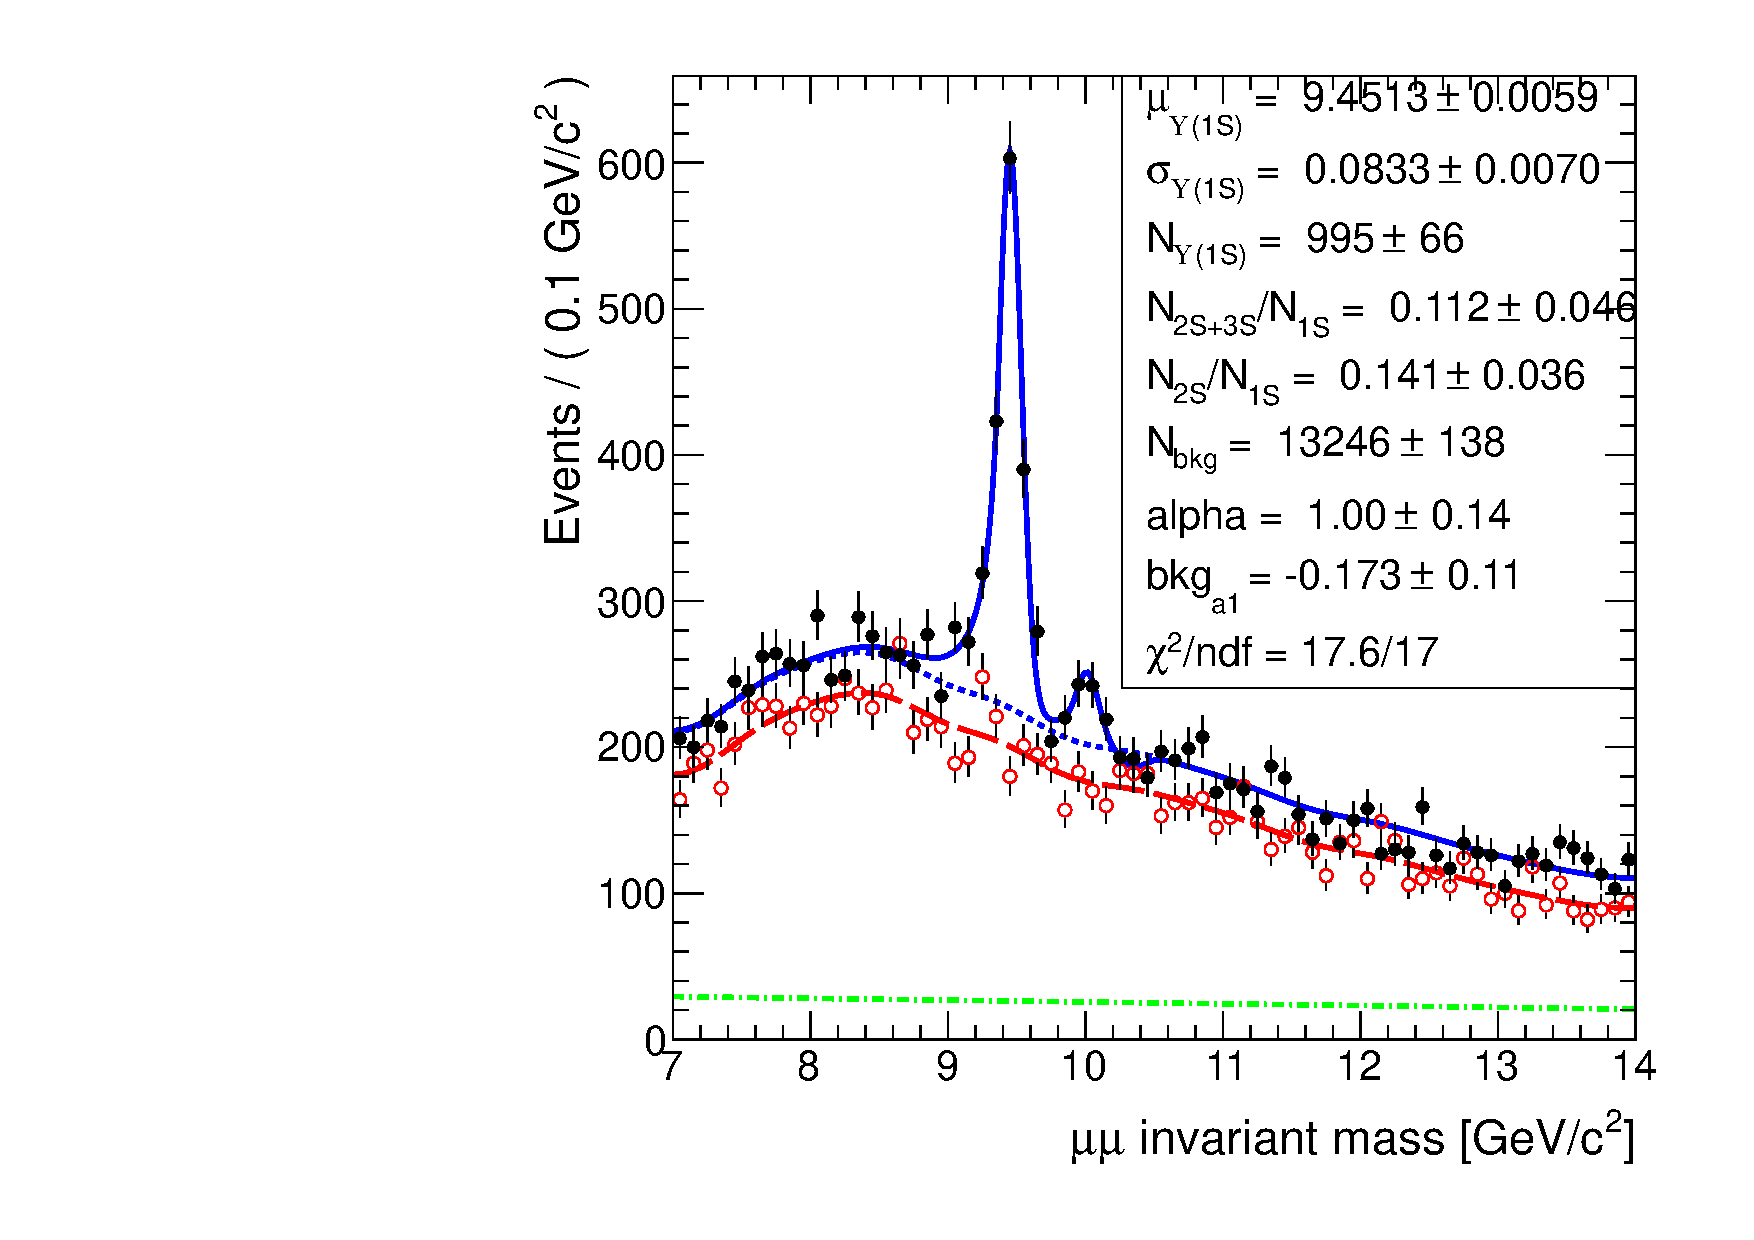
\includegraphics[angle=0,width=0.5\textwidth]{figures/fitting/masspeak_Hi_paramOn_MuonPT35_liner}}
    \subfigure[$\pt^\mu>4.0\GeVc$, rookeyspdf, $150 \mu b^{-1}$]{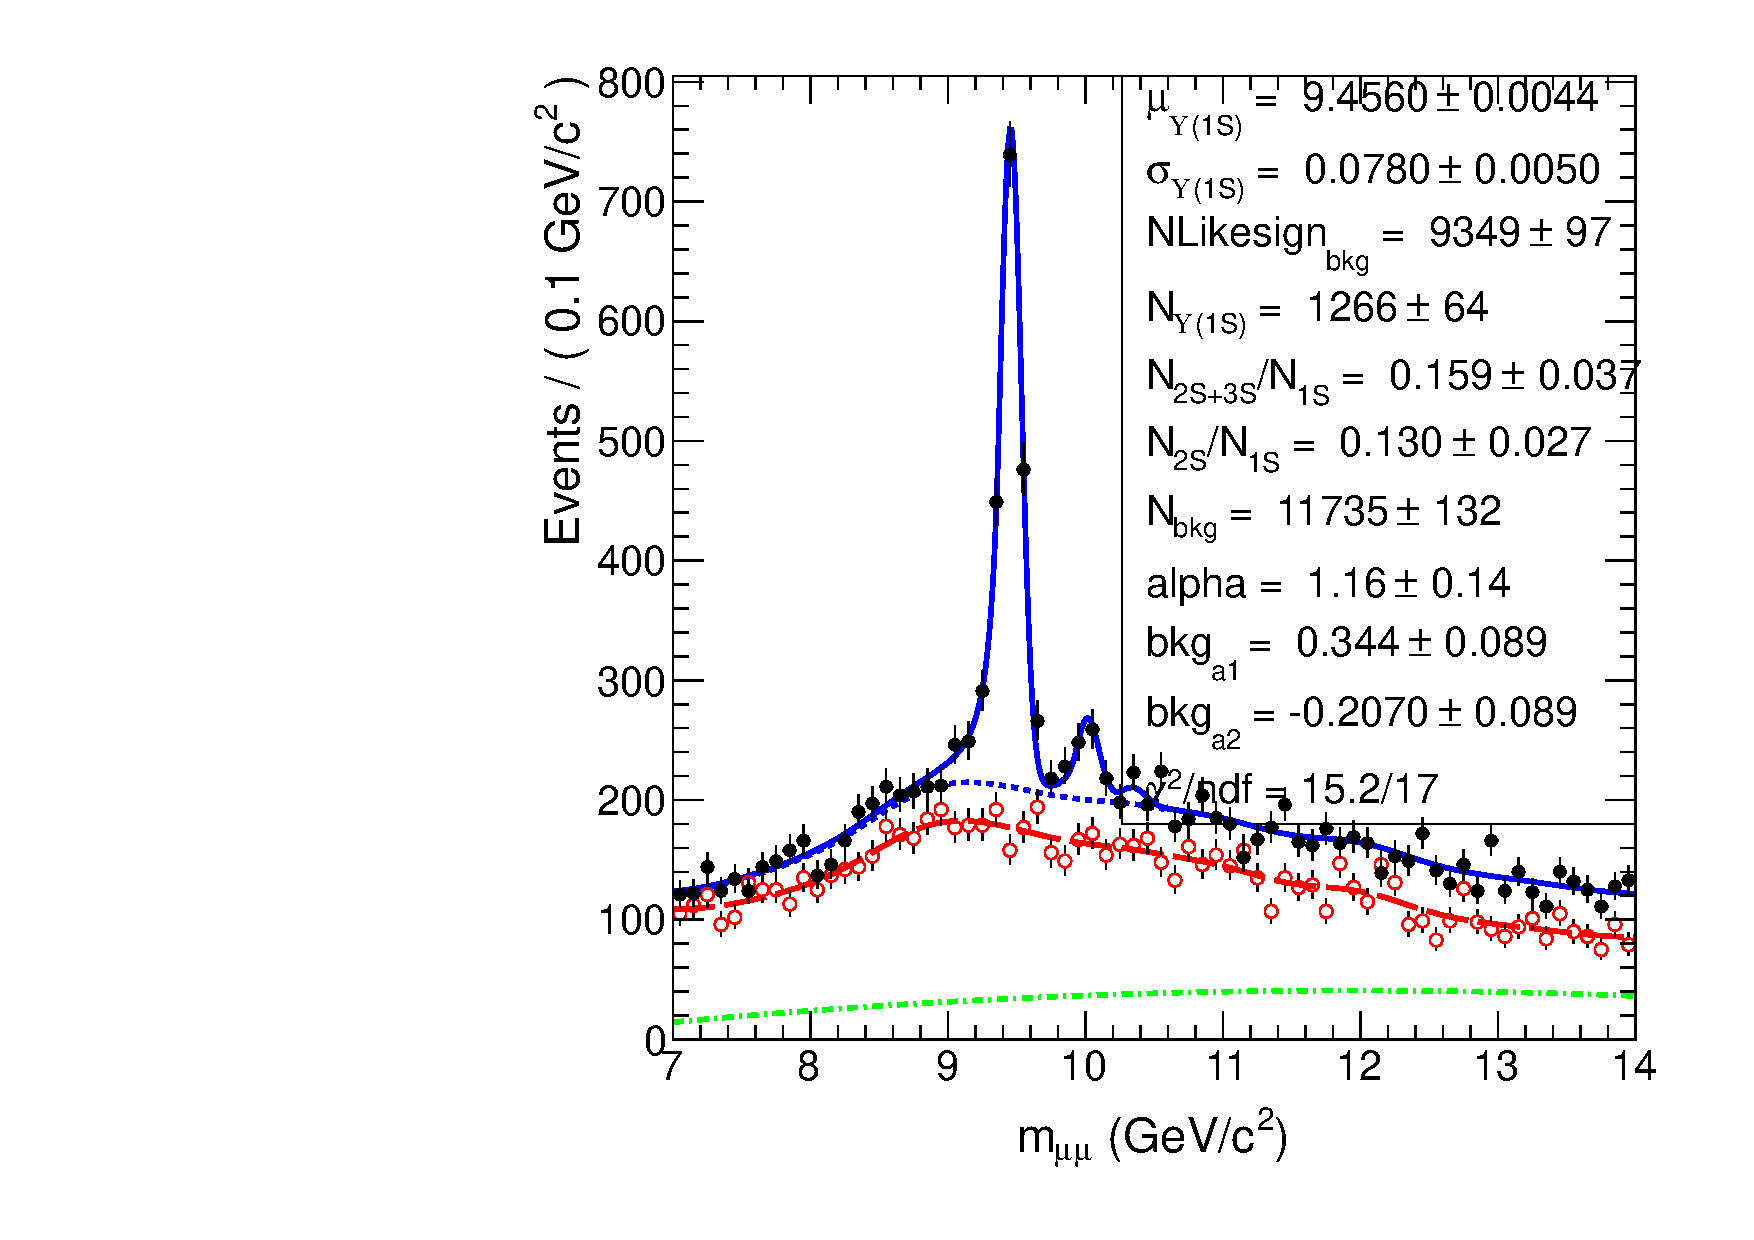
\includegraphics[angle=0,width=0.5\textwidth]{figures/fitting/masspeak_Hi_paramOn_liner}}\\
    \subfigure[$\pt^\mu>3.5\GeVc$,    exp*erf, $70 \mu b^{-1}$]{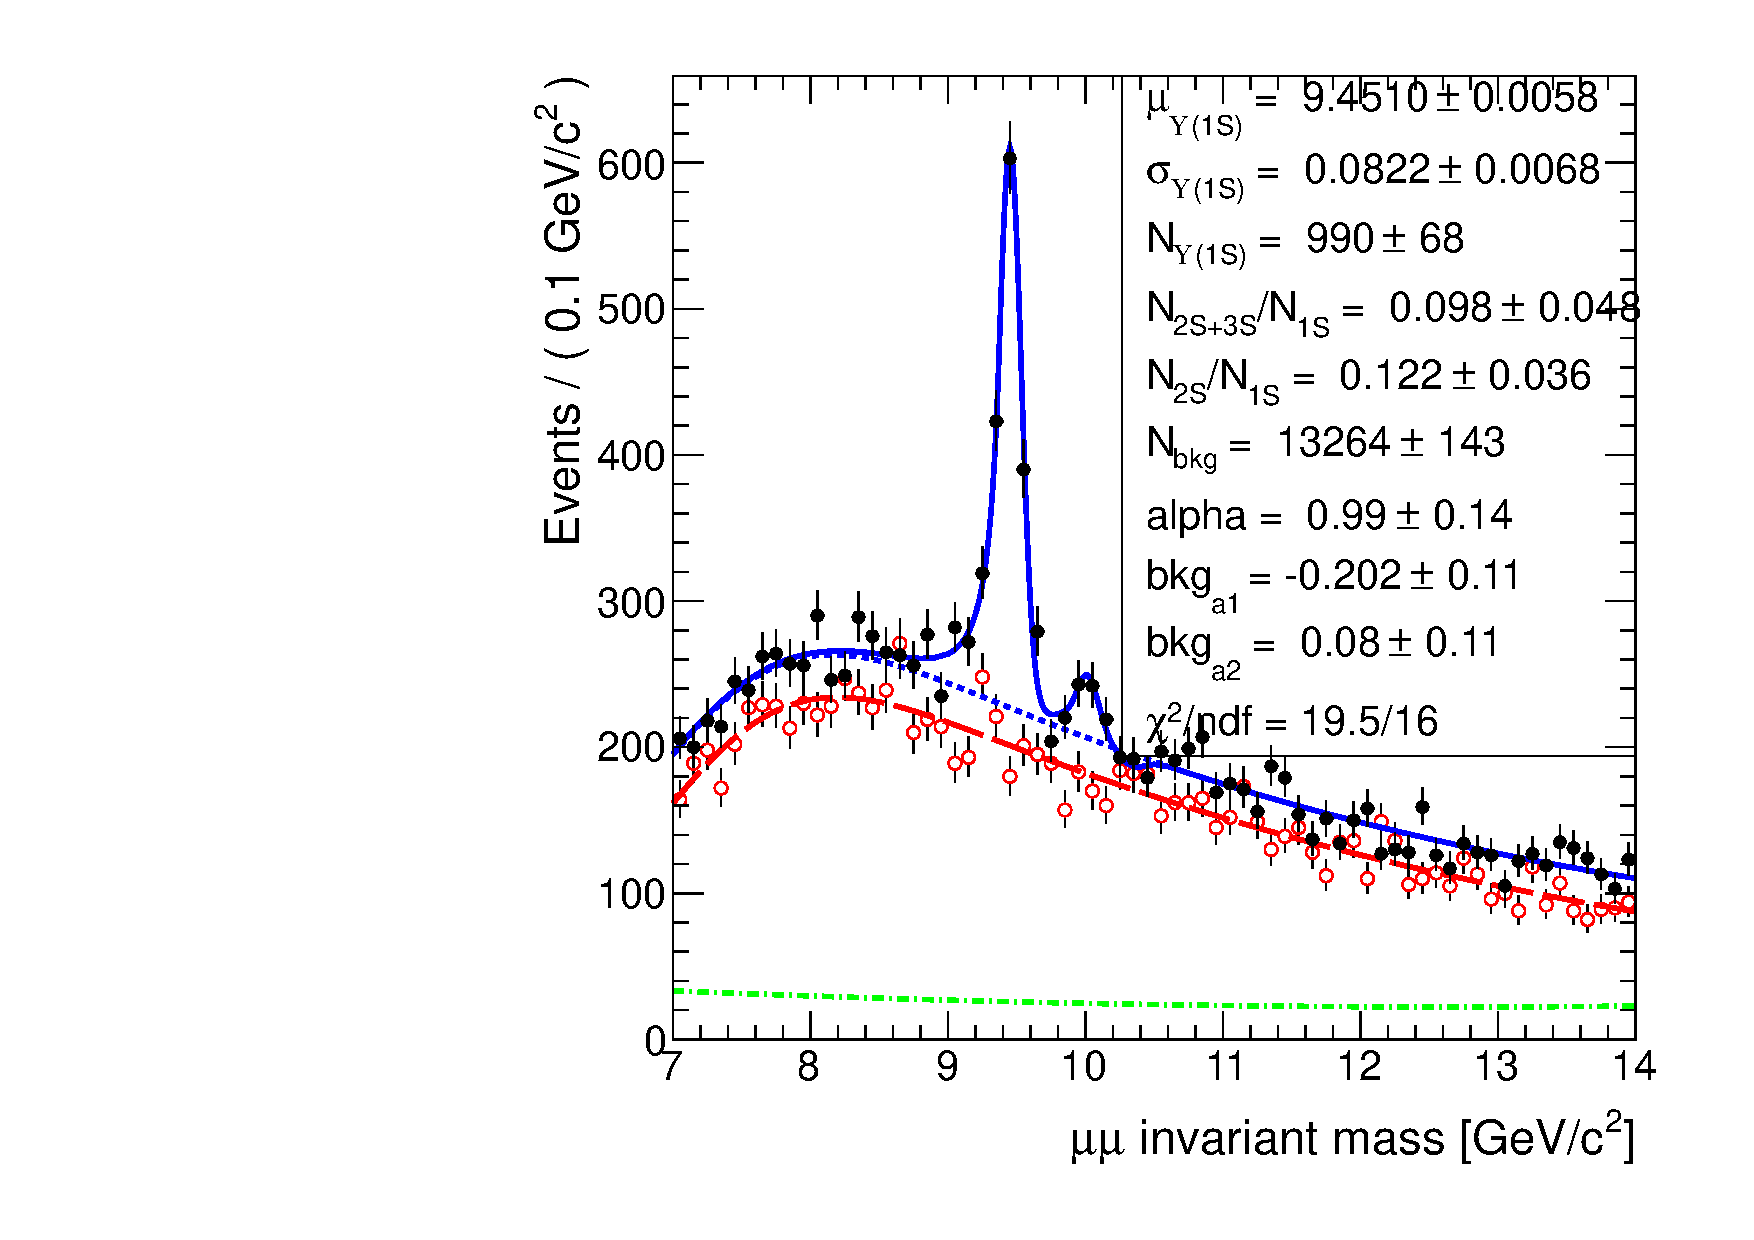
\includegraphics[angle=0,width=0.5\textwidth]{figures/fitting/masspeak_Hi_paramOn_ErrFunc_MuonPT35}}
    \subfigure[$\pt^\mu>4.0\GeVc$,    exp*erf, $150 \mu b^{-1}$]{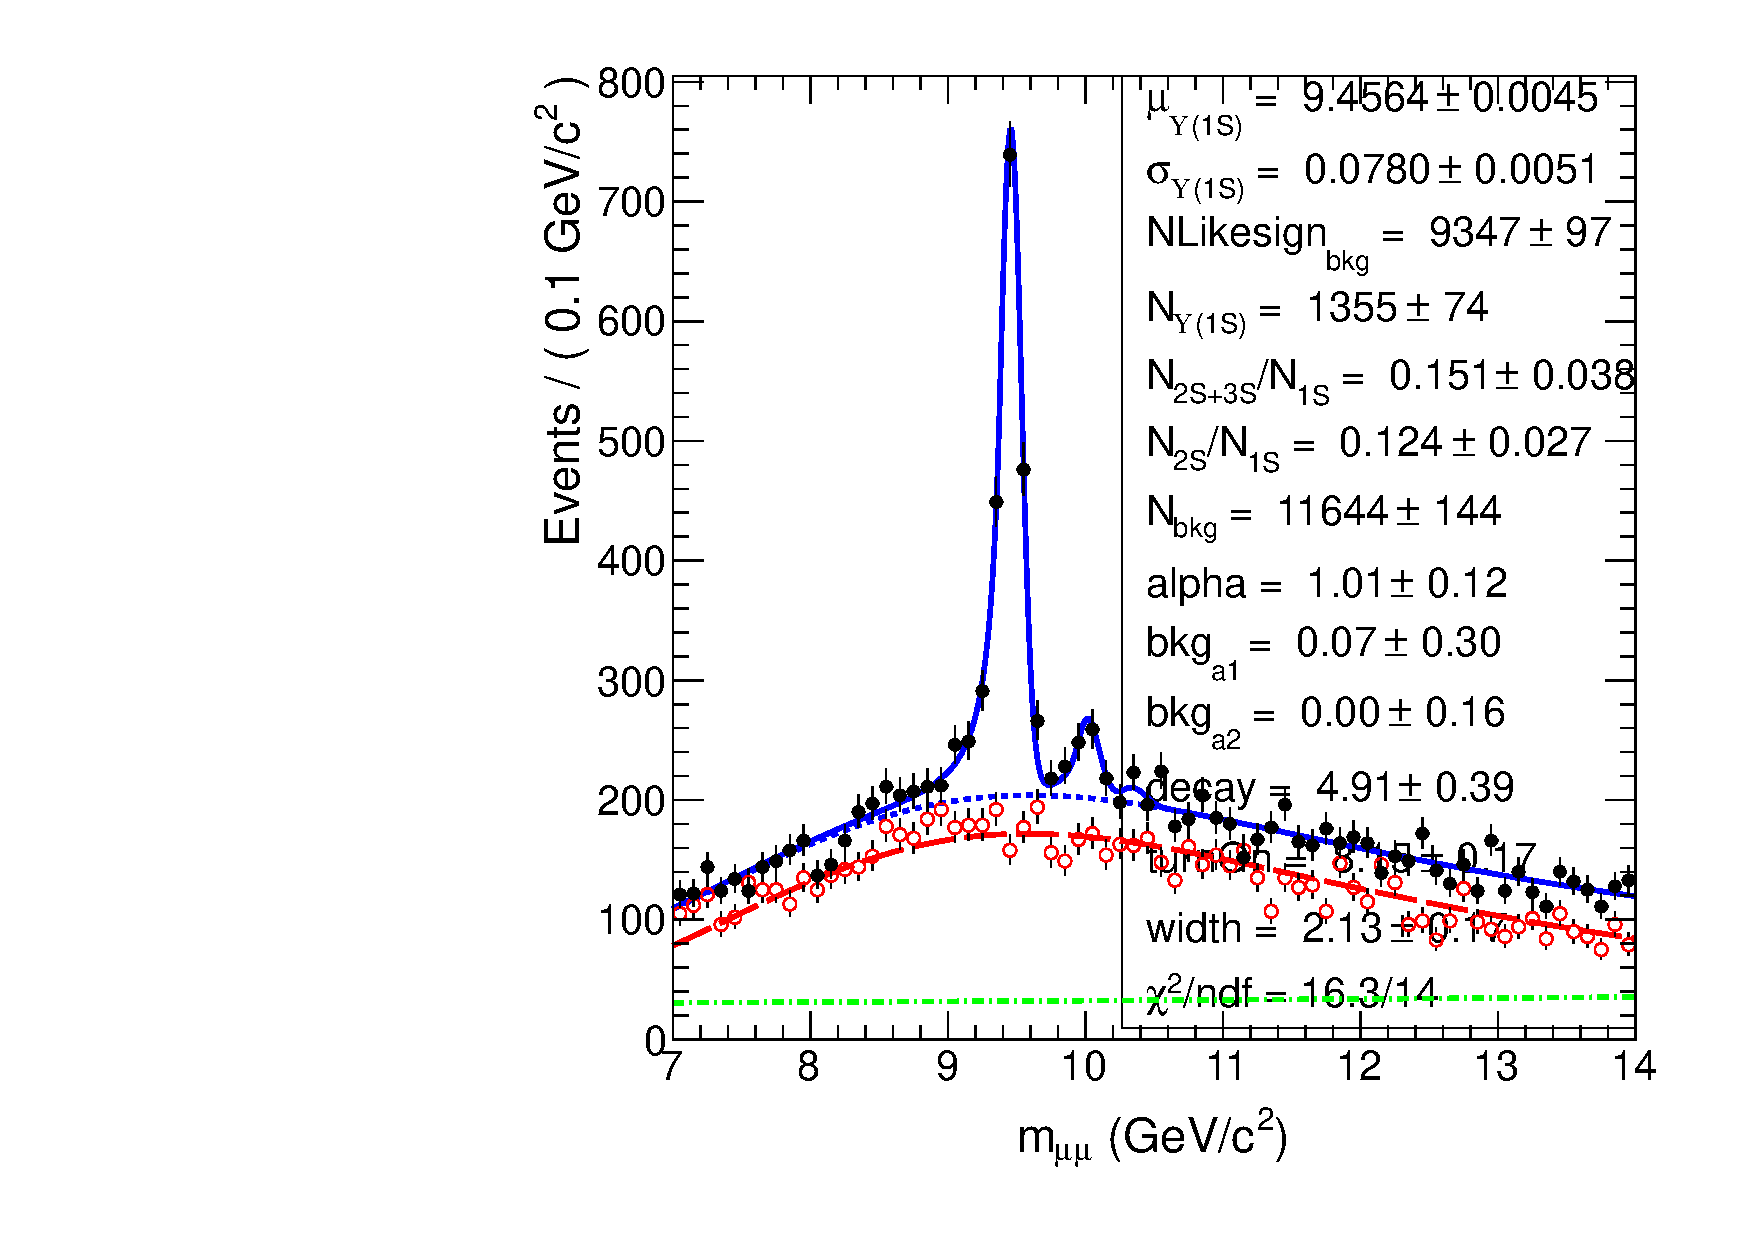
\includegraphics[angle=0,width=0.5\textwidth]{figures/fitting/masspeak_Hi_paramOn_ErrFunc}}
    \caption{Mass fits, with background constrained from like-sign dimuon spectrum.}
    \label{fig:massfits_likesign}
  \end{center}
\end{figure}

%\begin{figure}[hbtp]
%  \begin{center}
%    %\subfigure[]
%    {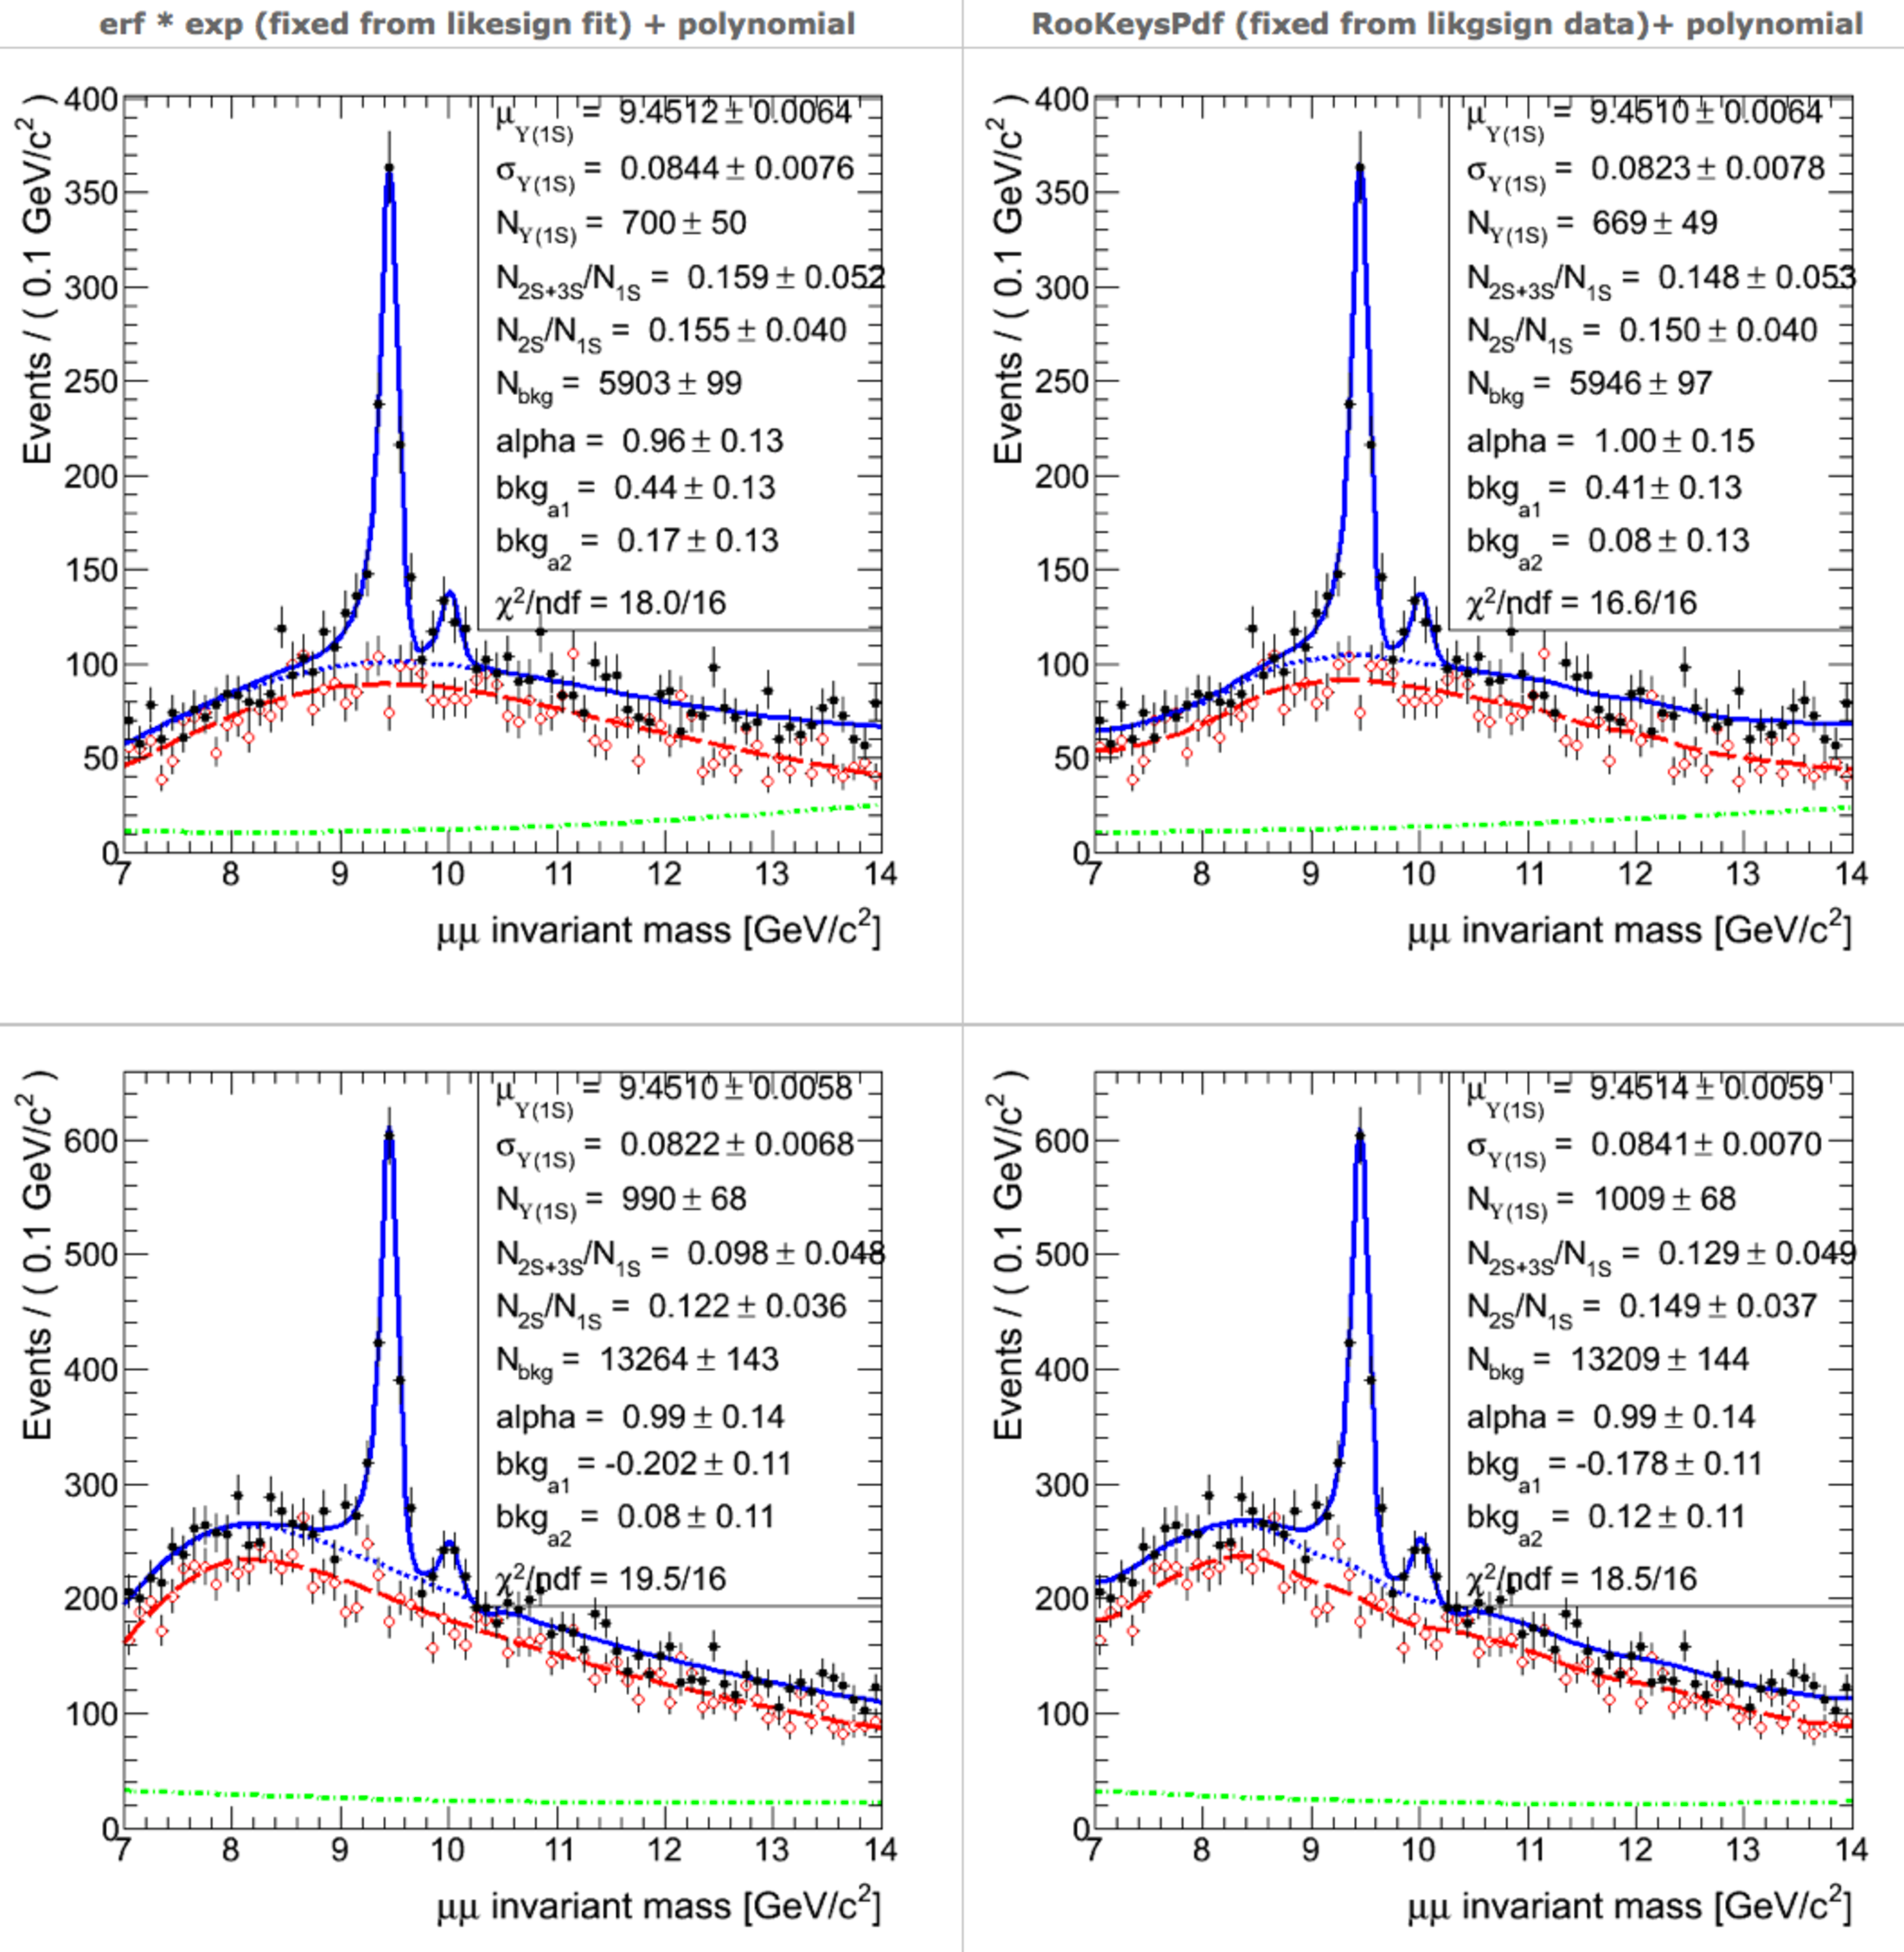
\includegraphics[angle=0,width=1\textwidth]{figures/fitting/massfits_likesign_option2}}
%    \caption{Mass fits, with background constrained from like-sign dimuon spectrum.}
%    \label{fig:massfits_likesign}
%  \end{center}
%\end{figure}



\subsubsection{Track-rotation method}
\label{sec:track-rotsation}

We explore an independent method to estimate the combinatorial background. 
This is normally referred to as ``track-rotation method'' and consists of the following steps:
(i) all like-sign muon pairs (or the unlike-sign muon pairs) in the event are formed, 
(ii) for each pair, one of the muons is randomly selected, and 
(iii) its $\phi$ coordinate is rotated by $\pi$. 
In this way we obtain an uncorrelated sample of tracks, extracted directly from the data and thus matching the data kinematics, 
from which the combinatorial mass distribution can be estimated. 

Having extracted the combinatorial background PDF, the same fitting strategy as described in Sec.~\ref{sec:like-sign} for the like-sign case is employed when fitting the oppositely charged dimuon data. The track rotation PDF is normalized to like-sign yield. 
The results are shown in~\fig{fig:track_rotation} for like-sign, in~\fig{fig:track_rotation_OS} for unlikesign. They display a good description of the data.
A comparison of like-sign pairs shape, track rotation pairs shape, and unlike-sign pairs shape is shown in~\fig{fig:compareBkgd}.

\begin{figure}[hbtp]
  \begin{center}
	\subfigure[erf*exp + pol.2]{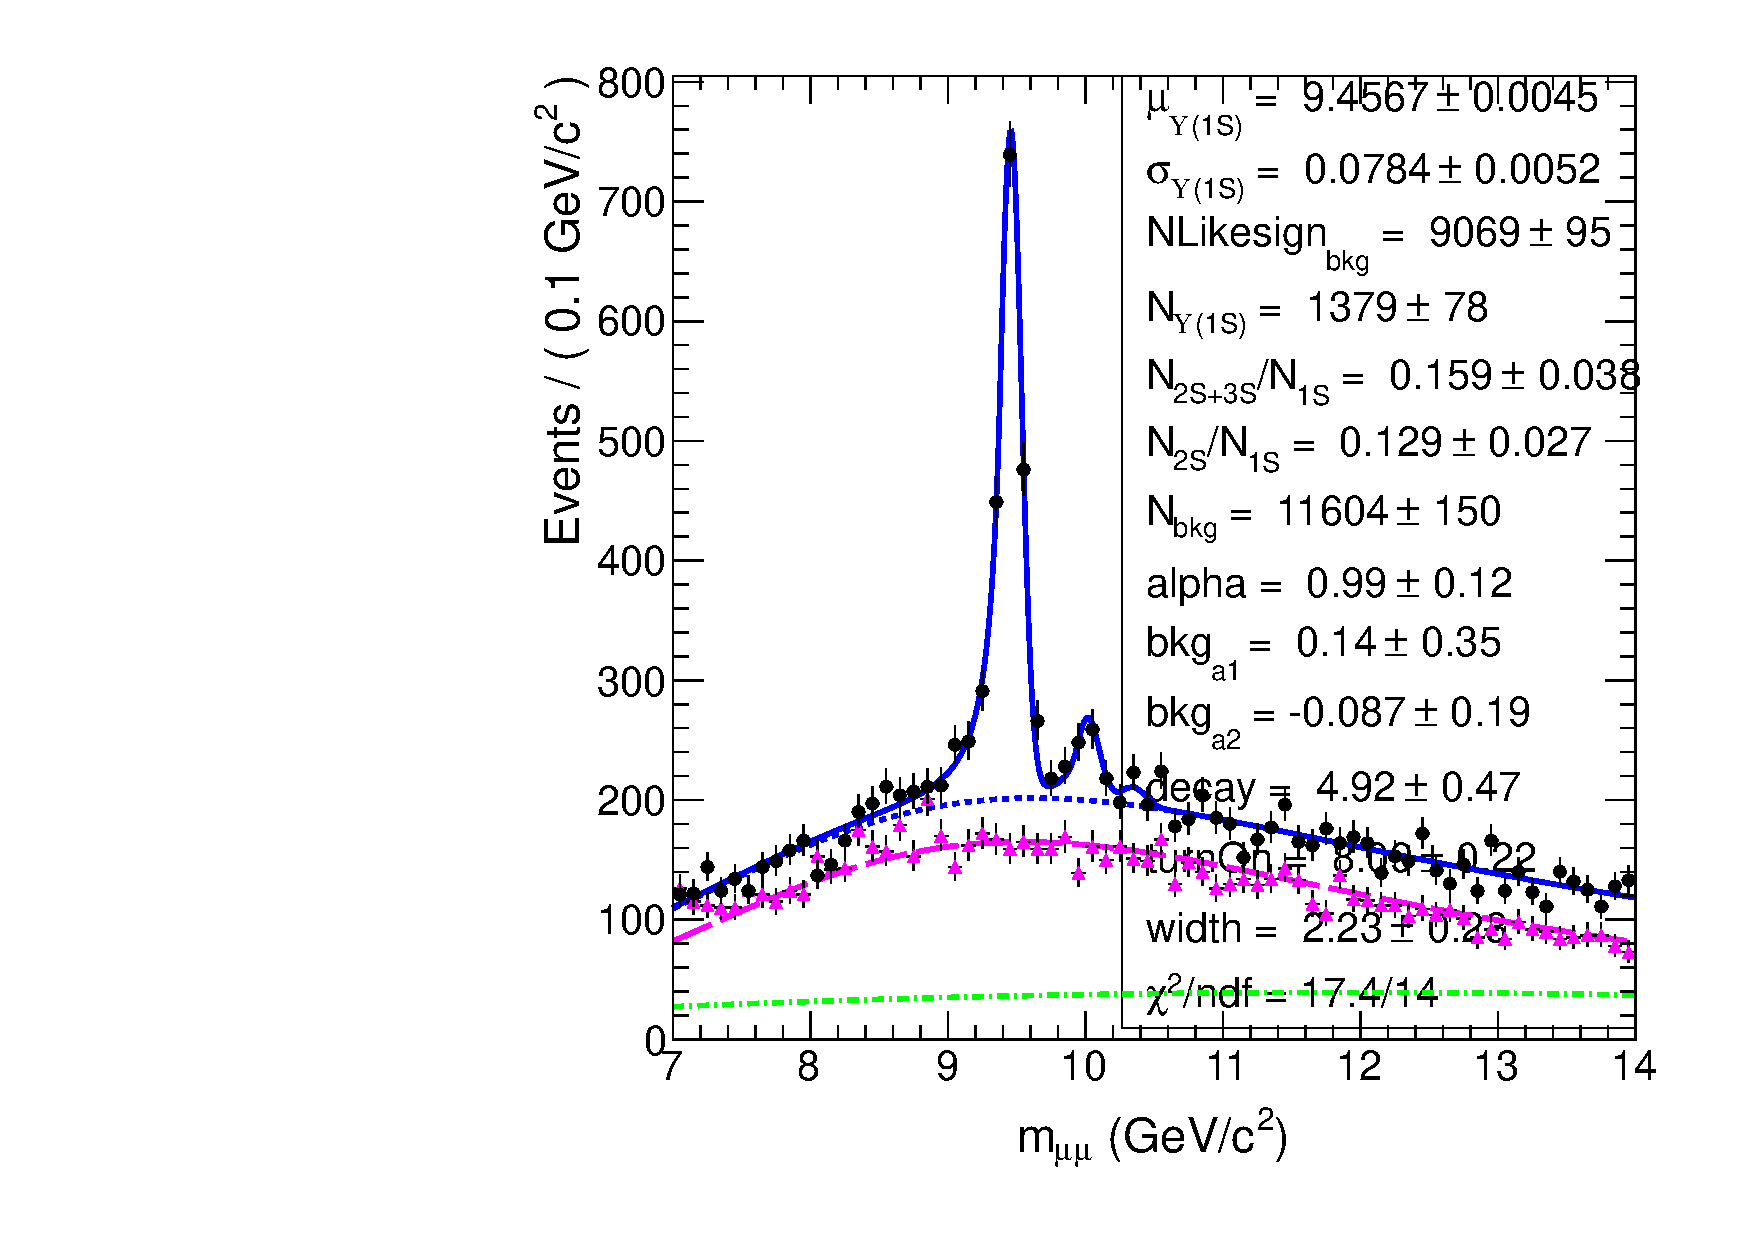
\includegraphics[angle=0,width=0.5\textwidth]{figures/fulldataset/masspeak_hi_TRerf.pdf}}
    \subfigure[keysPdf + pol.2]{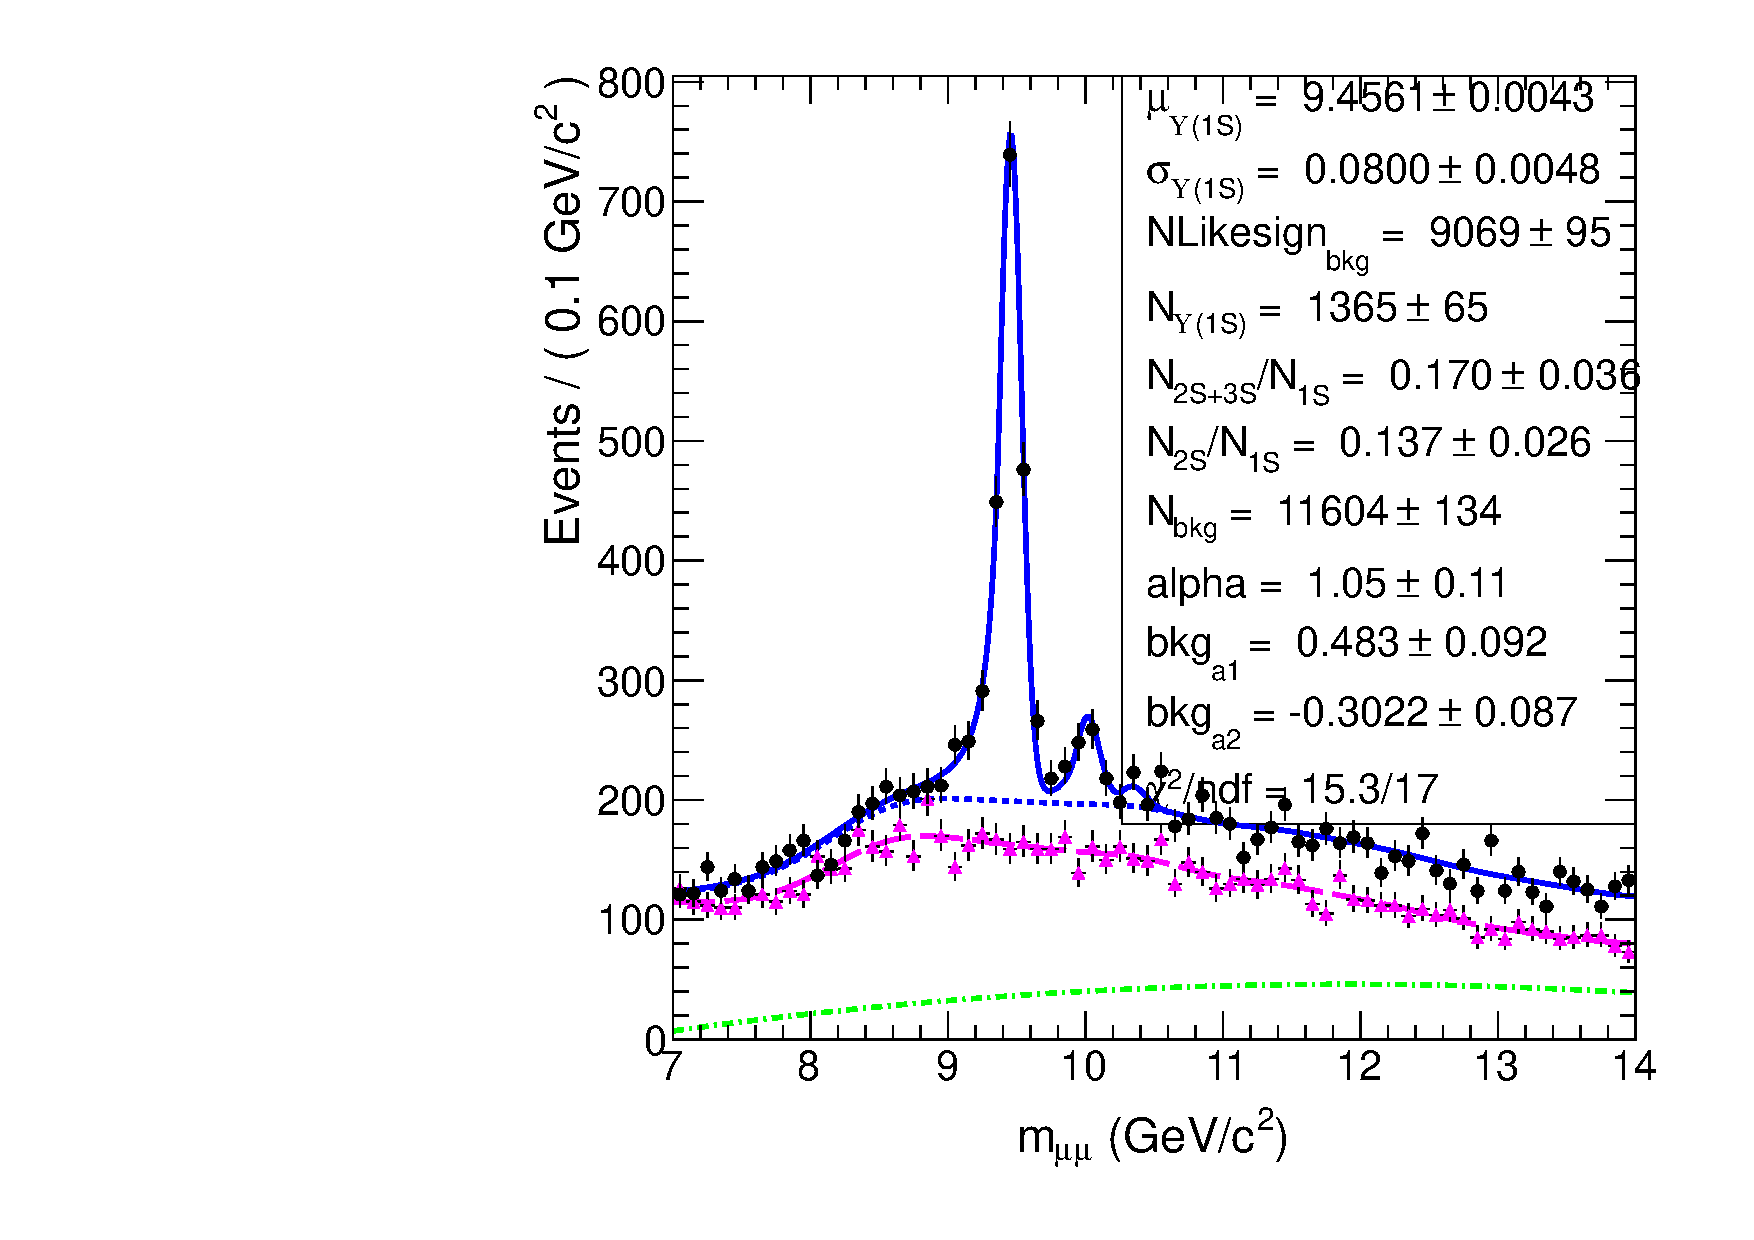
\includegraphics[angle=0,width=0.5\textwidth]{figures/fulldataset/masspeak_hi_TRkeys.pdf}}
    \caption{Mass fit, with background constrained from the track-rotated like-sign dimuon spectrum shown in magenta ($\pt^\mu>4.0\GeVc$, $150 \mu b^{-1}$).}
    \label{fig:track_rotation}
  \end{center}
\end{figure}

\begin{figure}[hbtp]
  \begin{center}
    \subfigure[erf*exp + pol.2]{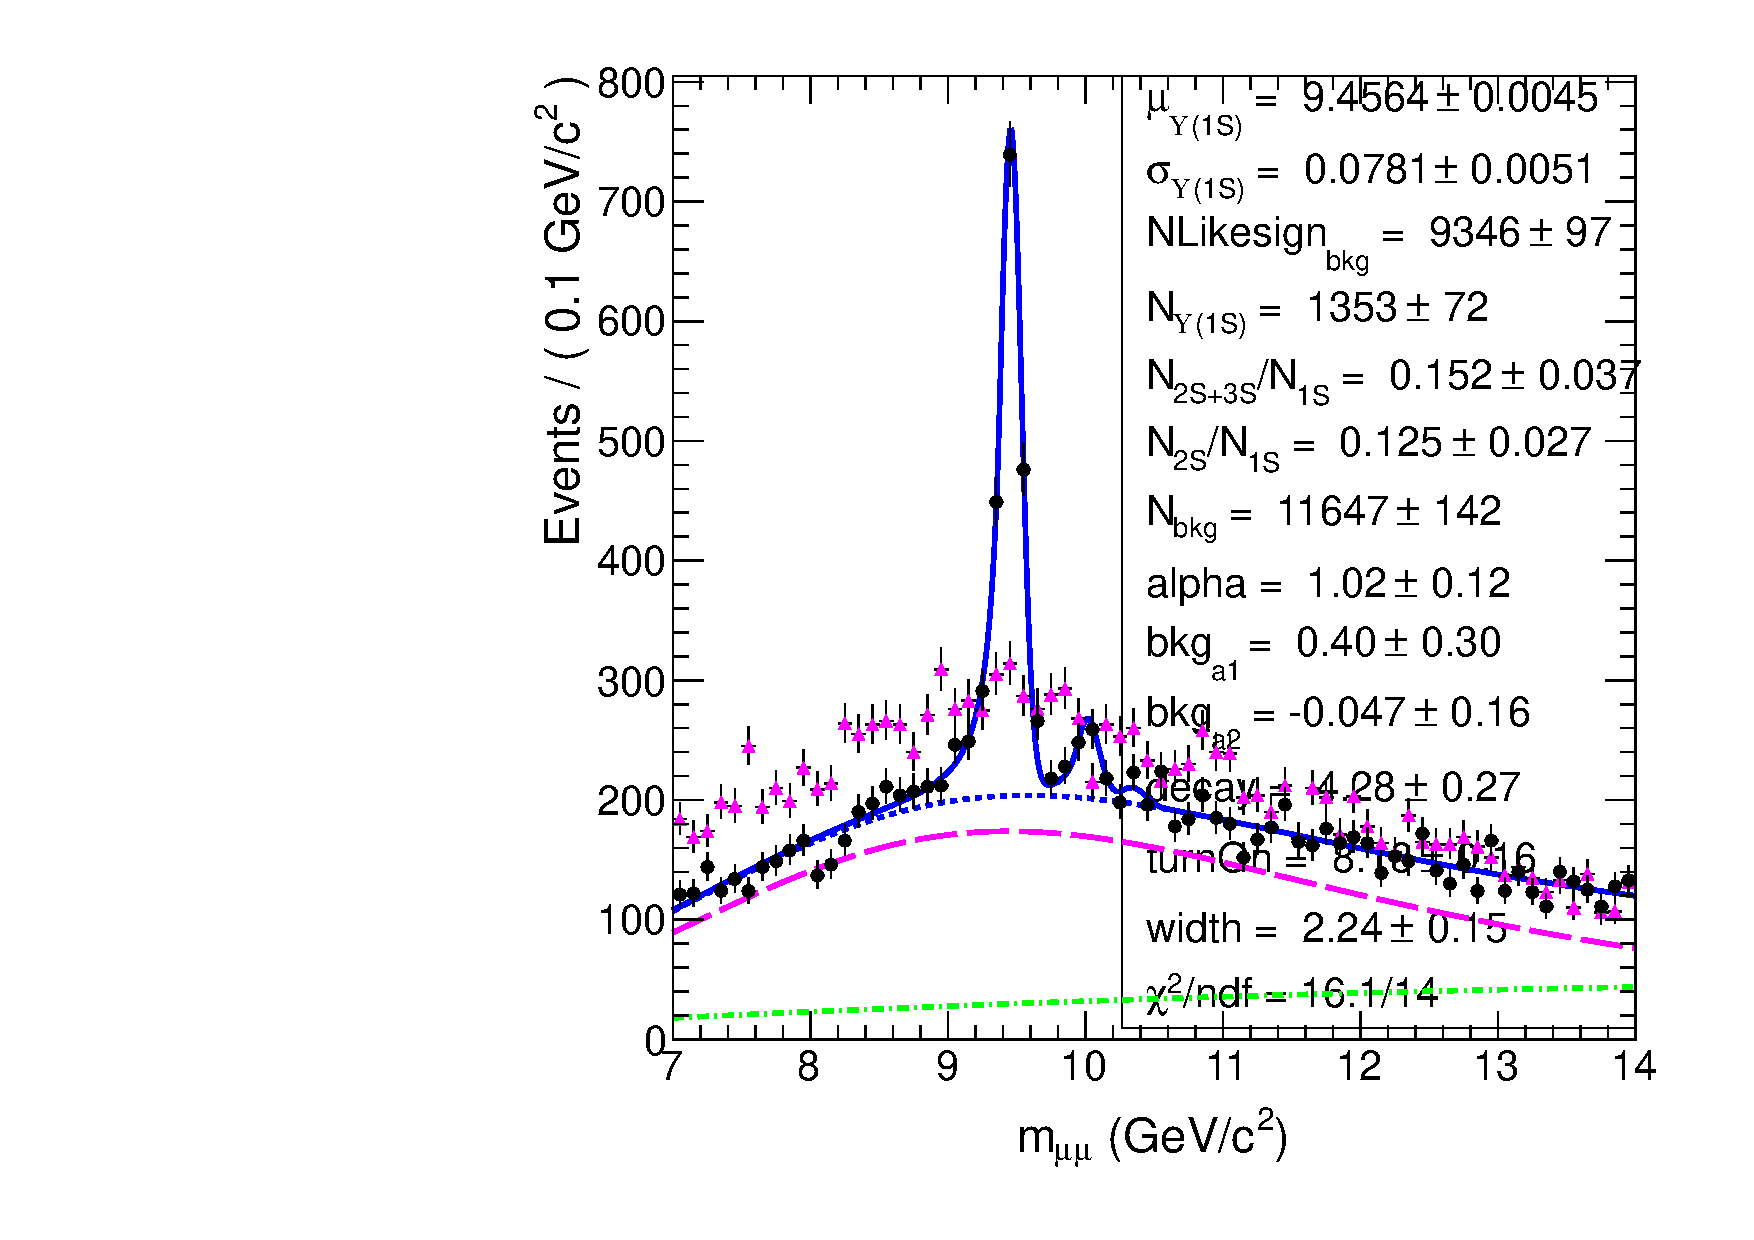
\includegraphics[angle=0,width=0.5\textwidth]{figures/fulldataset/masspeak_Hi_paramOn_OS_trkRot.pdf}}
    \subfigure[keysPdf + pol.2]{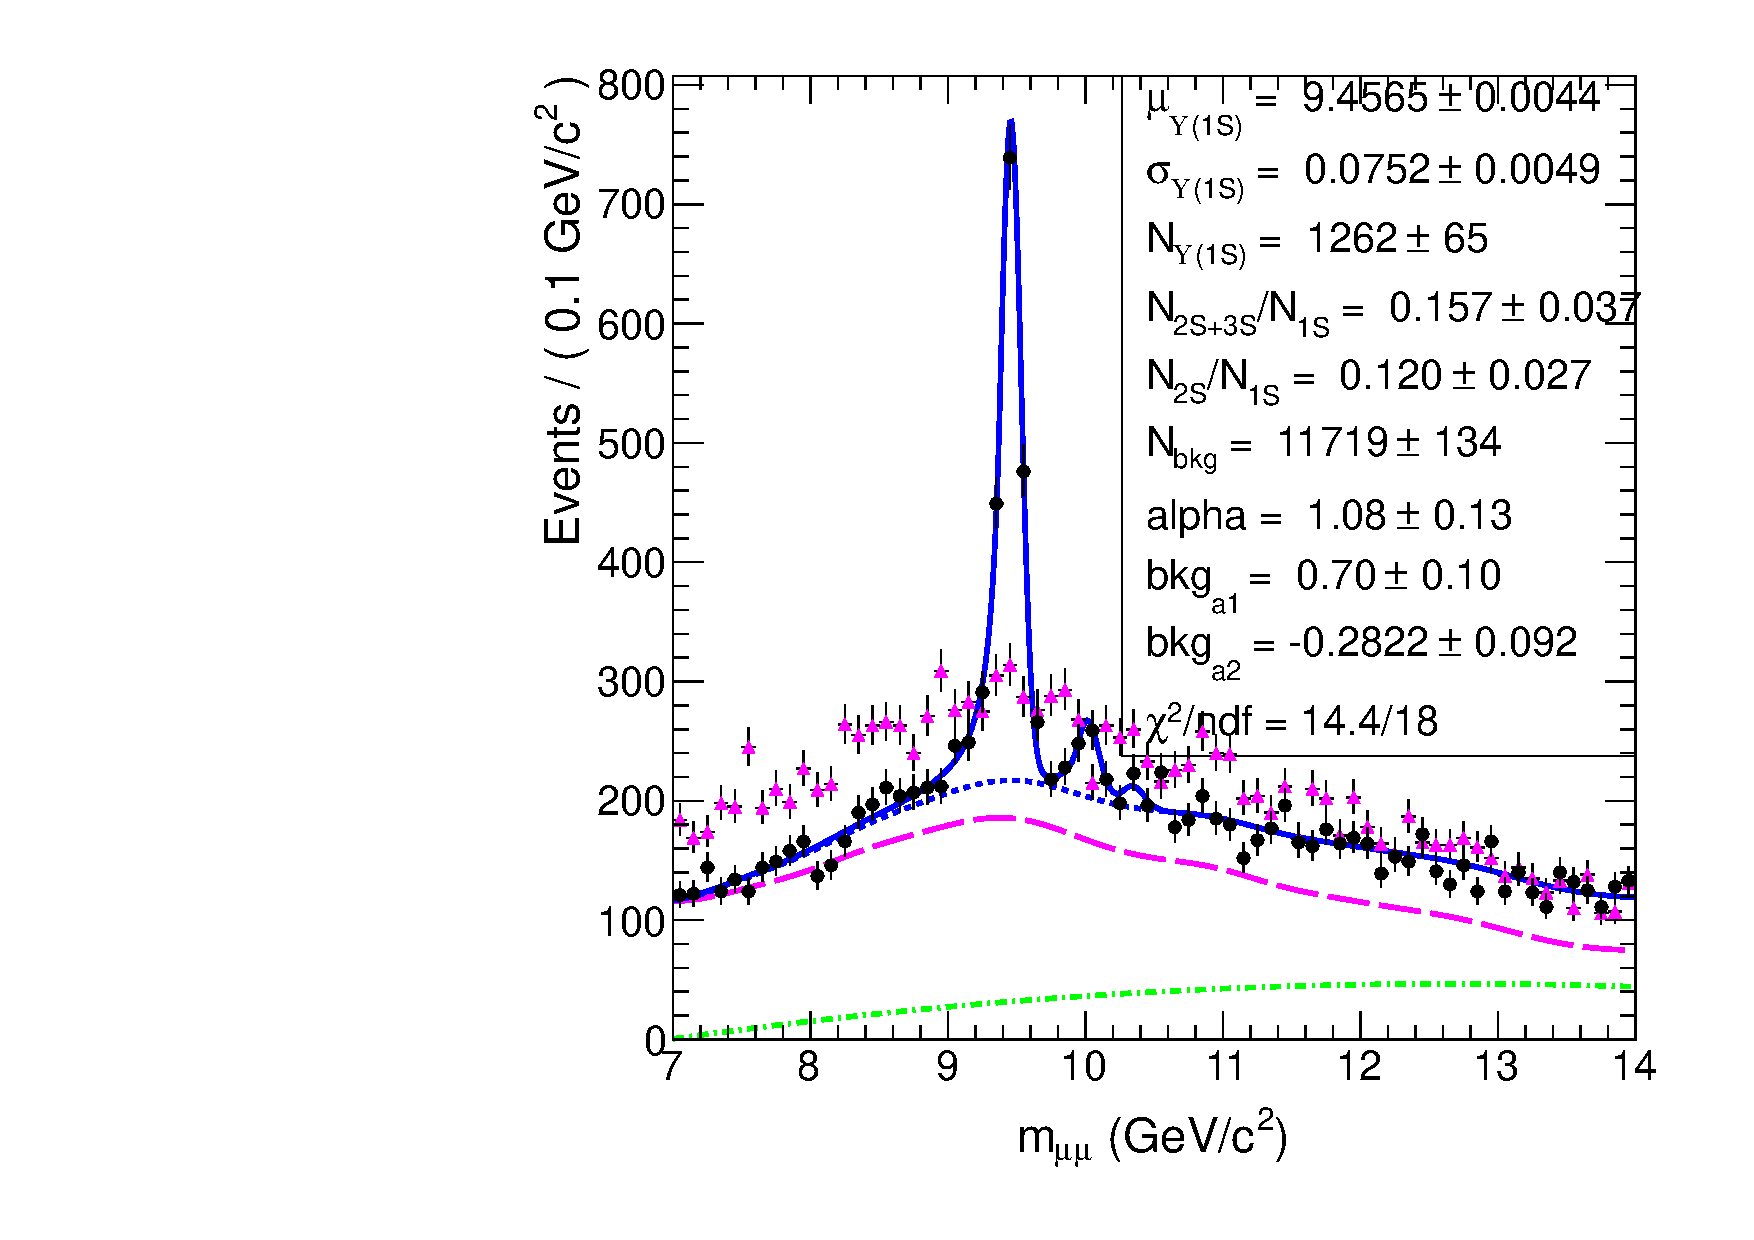
\includegraphics[angle=0,width=0.5\textwidth]{figures/fulldataset/masspeak_Hi_keysPdf_OS_trkRot.pdf}}
    \caption{Mass fit, with background constrained from the track-rotated unlike-sign dimuon spectrum shown in magenta points. The magenta curve is normalized to like-sign pairs yield.}
    \label{fig:track_rotation_OS}
  \end{center}
\end{figure}

\begin{figure}[h!]
 \begin{center}
    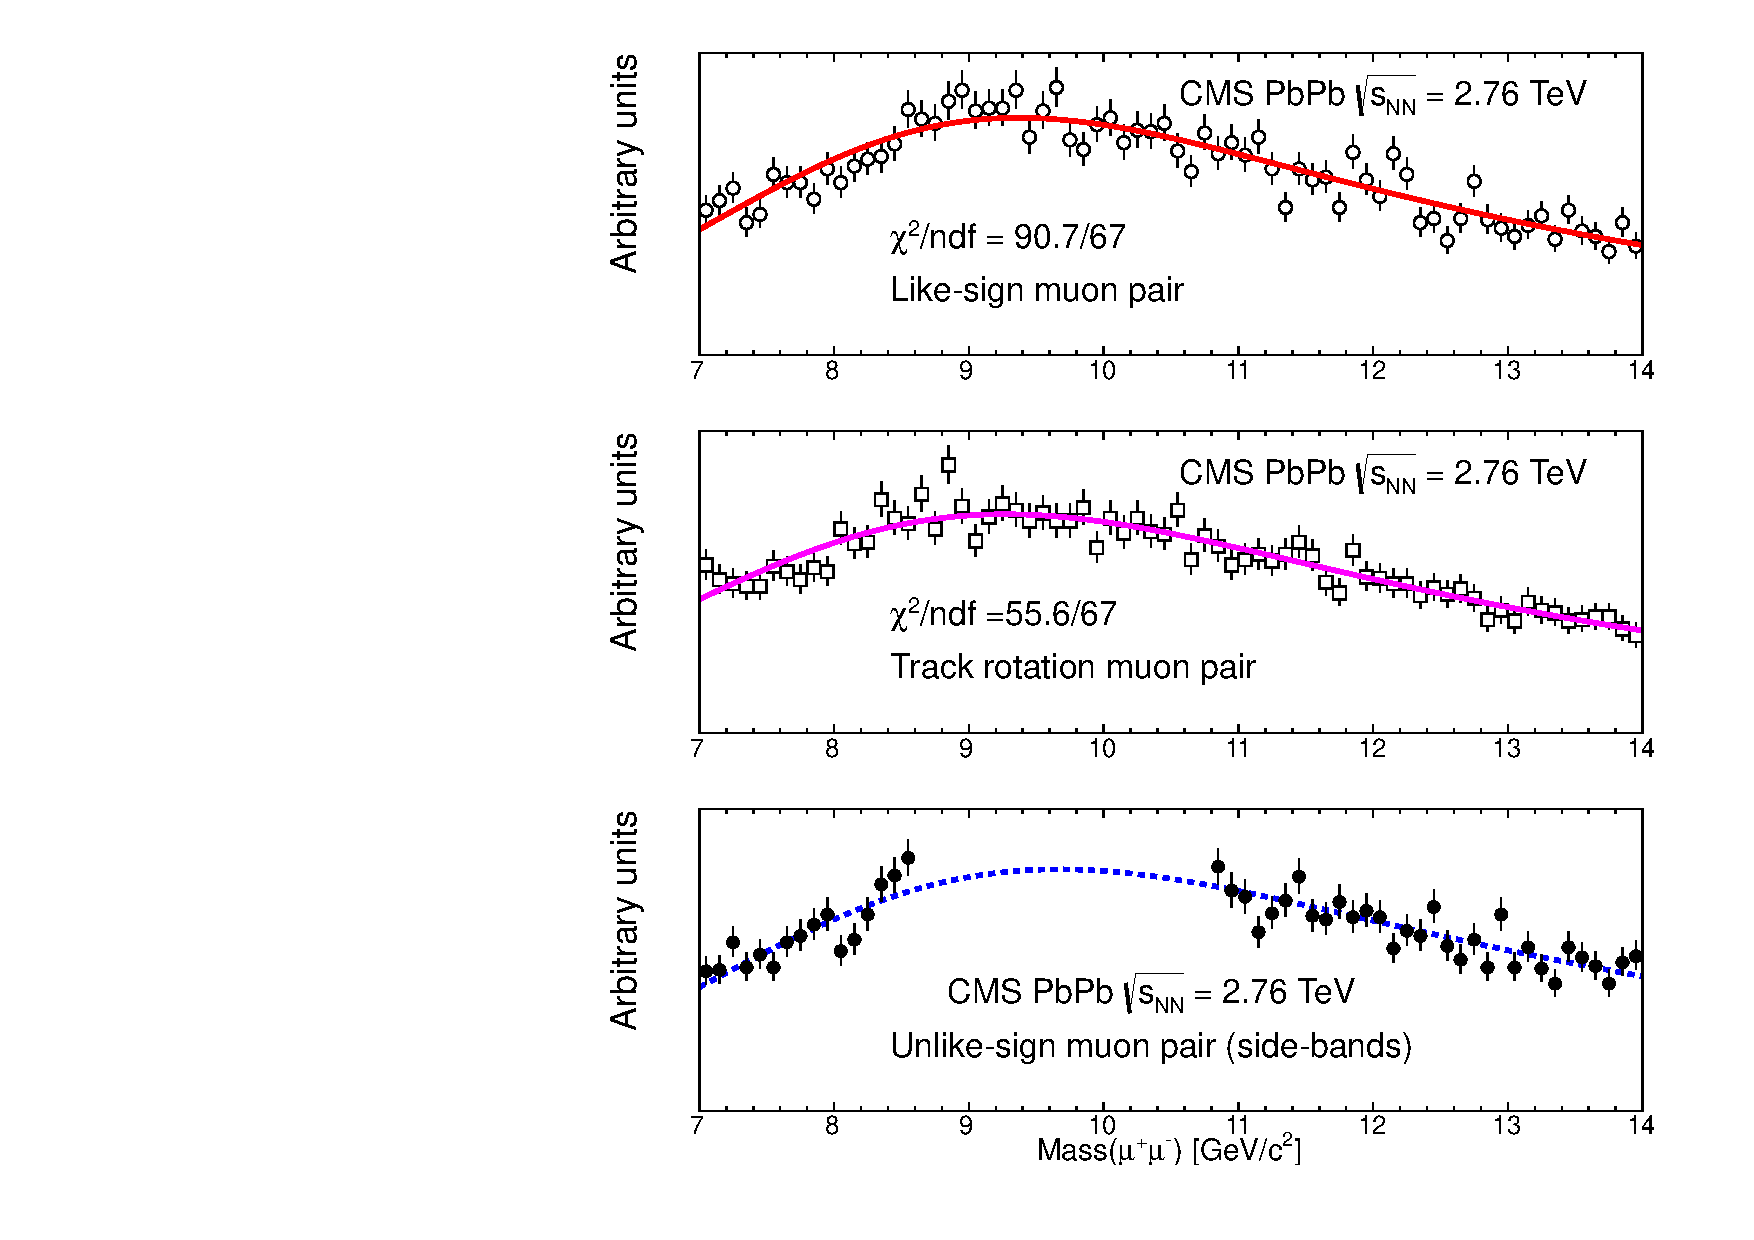
\includegraphics[angle=0,width=0.6\textwidth]{figures/fitting/plot3canvas.pdf}
    \caption{Compare like-sign, track rotation, and unlike-sign pairs}
    \label{fig:compareBkgd}
 \end{center}
\end{figure}

\subsection{Fits to the pp data}

The \pp 2.76 TeV dataset is the same as employed in the previous measurement~\cite{prl}. 
The same background fitting model as employed therein is adopted as nominal for the \pp case: 
second order polynomial. 

% https://espace.cern.ch/cms-heavyion/upsilon/fitting/ppdata.aspx

The same fitting model as devised for the \PbPb dataset is applied to the \pp dataset as well, to probe stability.  
Fit results are shown in \fig{fig:massfits_pp_nominal_all} for the nominal background model (error function times exponential), 
and in \fig{fig:massfits_pp_likesign} for fits utilizing like-sign information. 
The results are displayed for the $\pt^\mu>3.5\GeVc$ and $\pt^\mu>4.0\GeVc$ selections, 
and for the cases where the signal shape parameters are left floating and are fixed to the PbPb results.  
%
Despite the excessive number of parameters of the background model, when applied to the limited-statistics \pp dataset, the fit results show a fair stability. 


\begin{figure}[hbtp]
  \begin{center}
    \subfigure[$\pt^\mu>3.5\GeVc$]{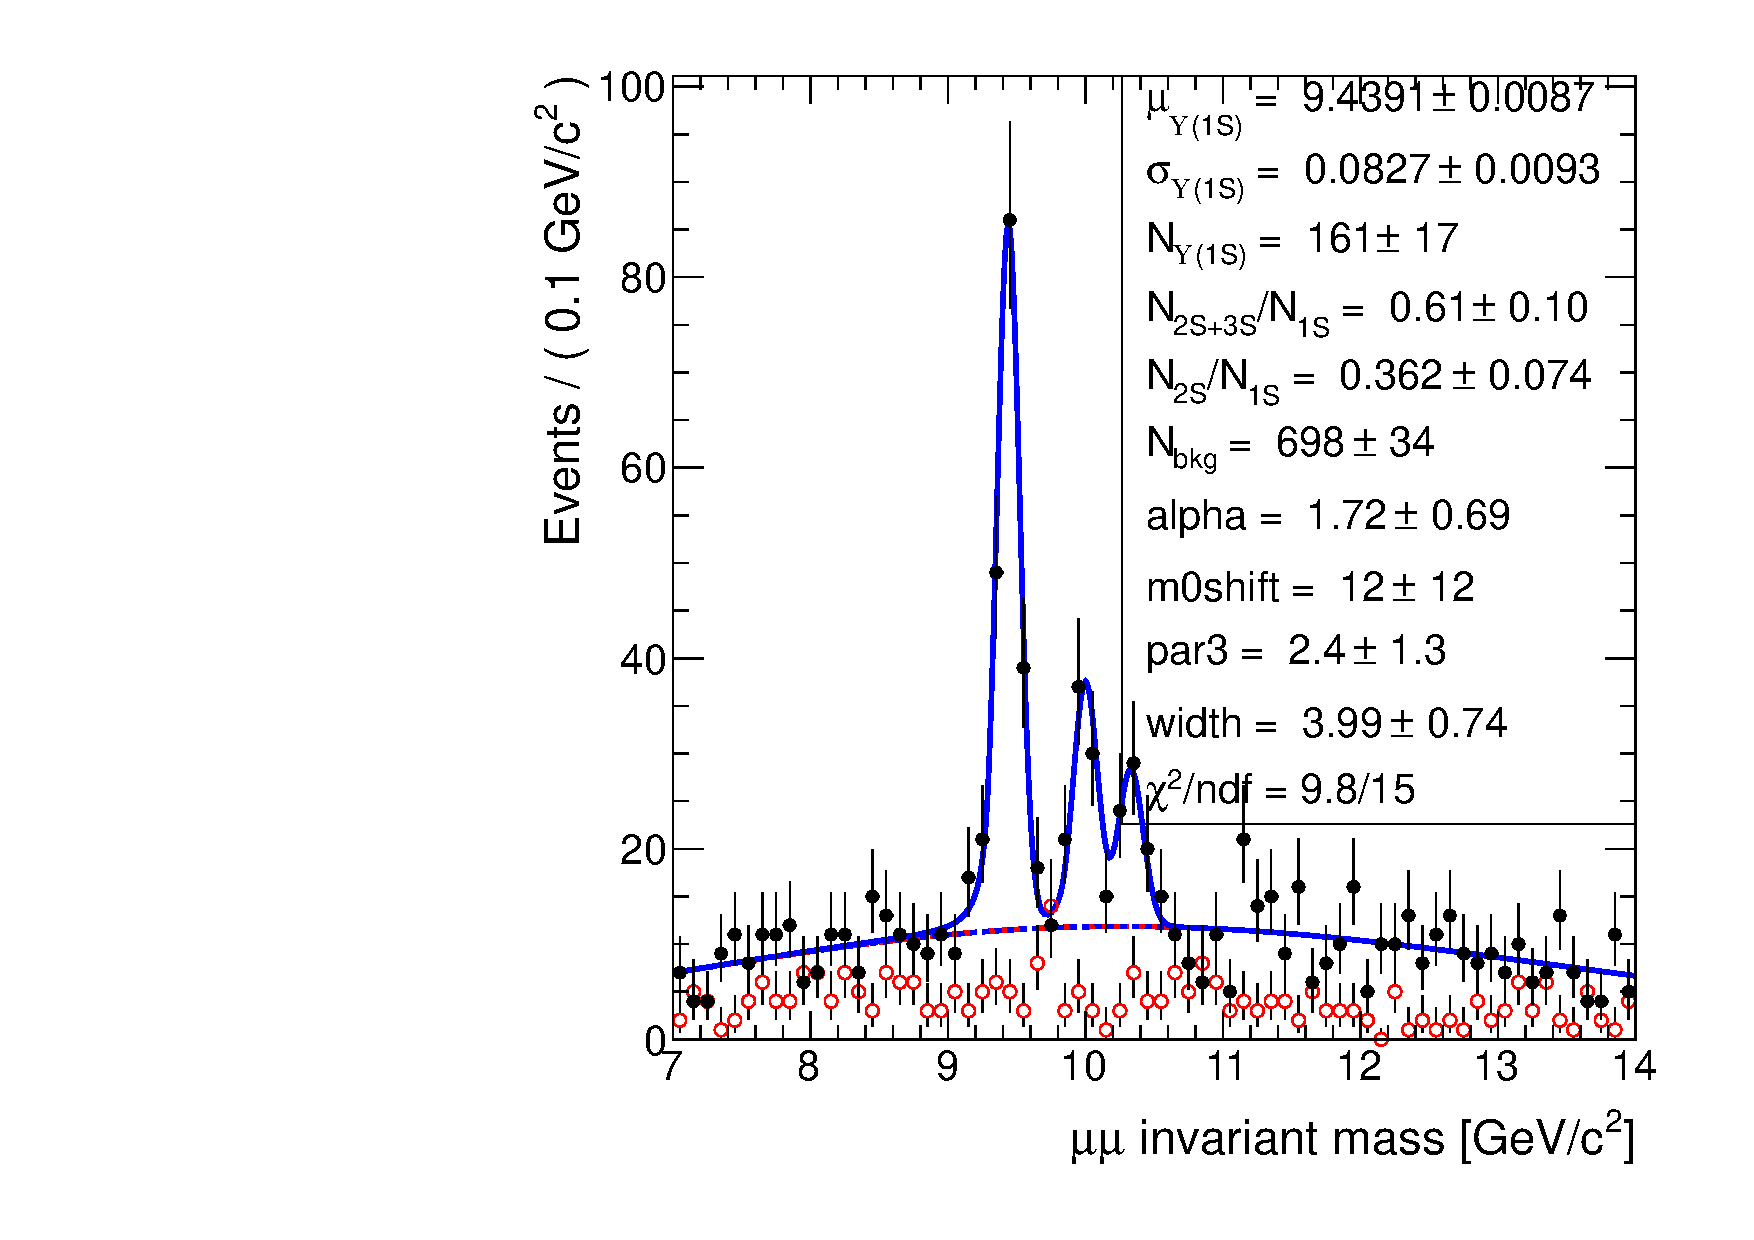
\includegraphics[angle=0,width=0.5\textwidth]{figures/pp276/masspeak_pp_HIrereco_erf_paramOn_MuonPT35}\label{fig:massfits_pp_nominal}}
    \subfigure[$\pt^\mu>4.0\GeVc$]{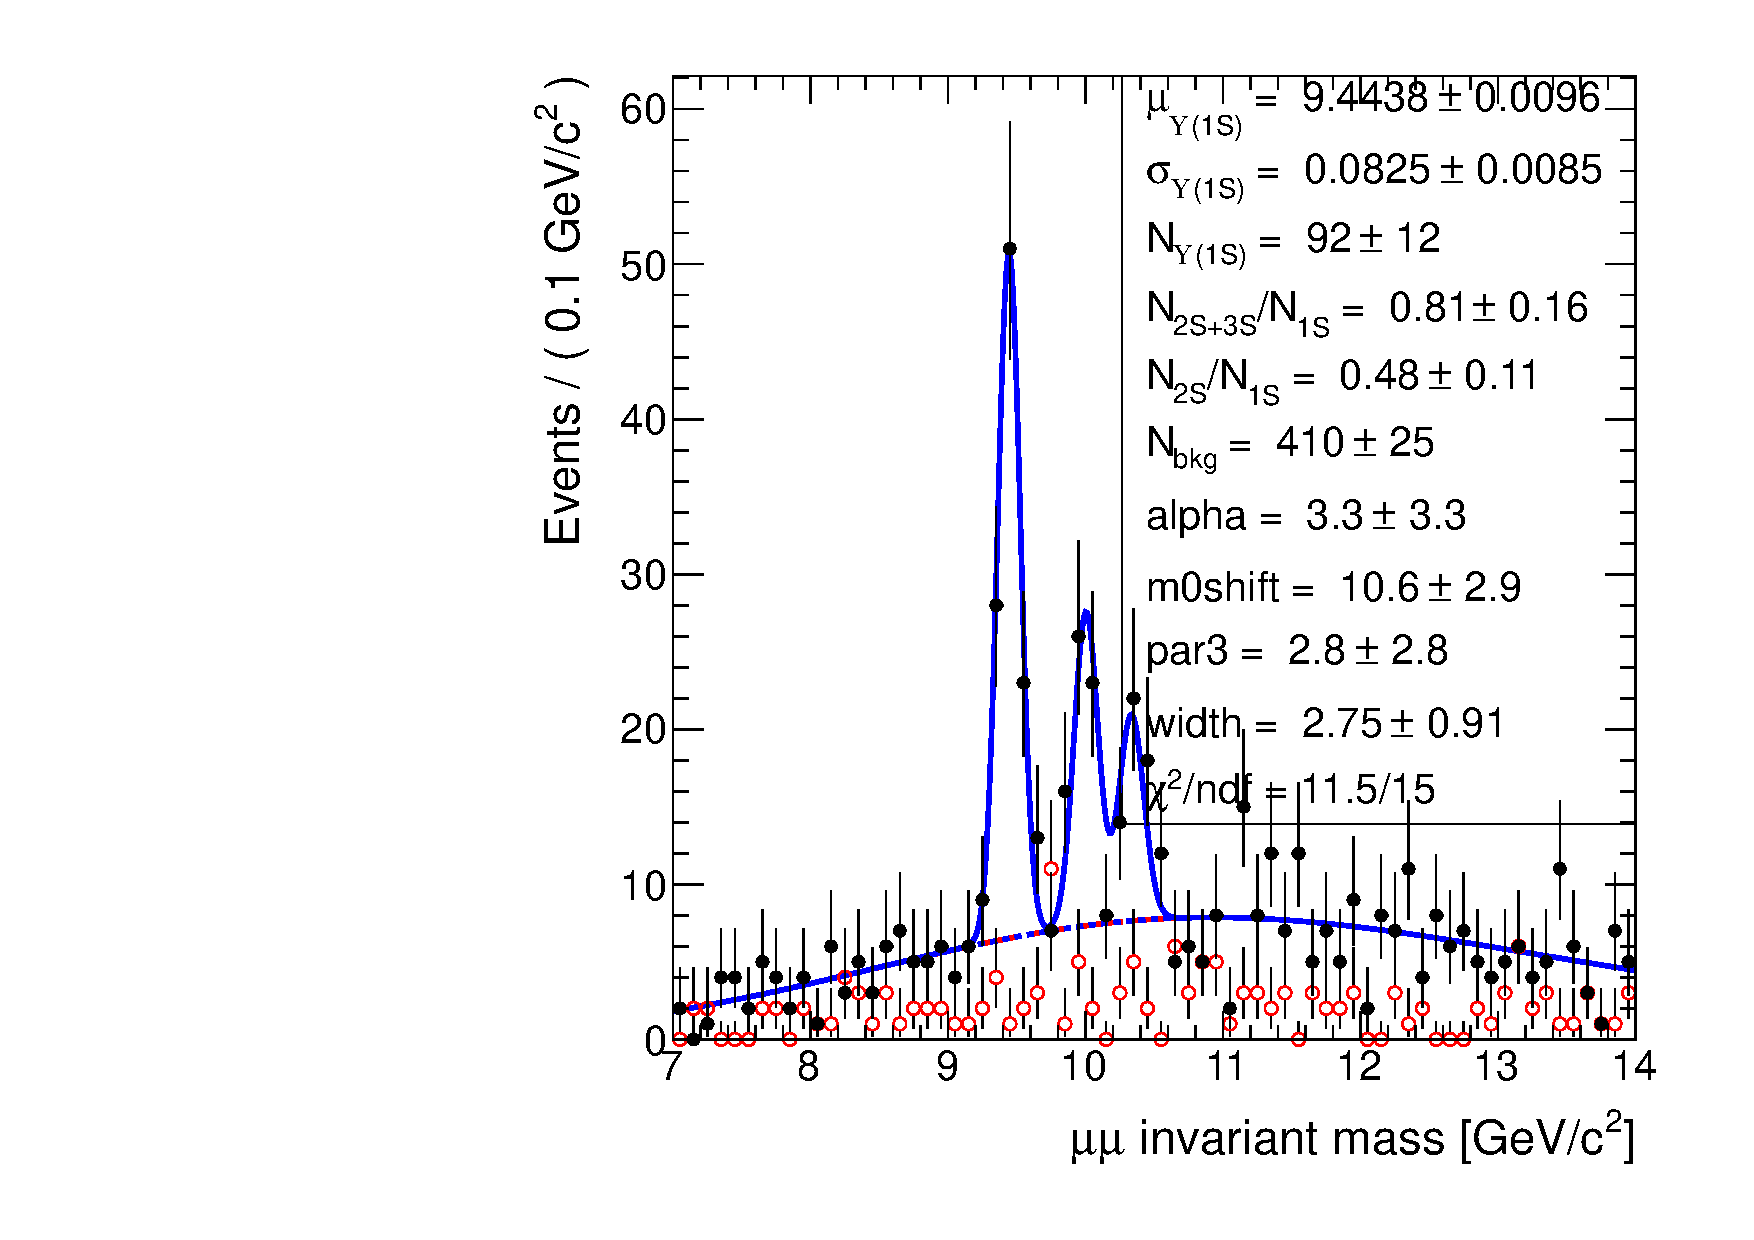
\includegraphics[angle=0,width=0.5\textwidth]{figures/pp276/masspeak_pp_HIrereco_erf_paramOn}\label{fig:massfits_pp_erf}}\\
    \subfigure[$\pt^\mu>3.5\GeVc$; signal shape fixed to PbPb]{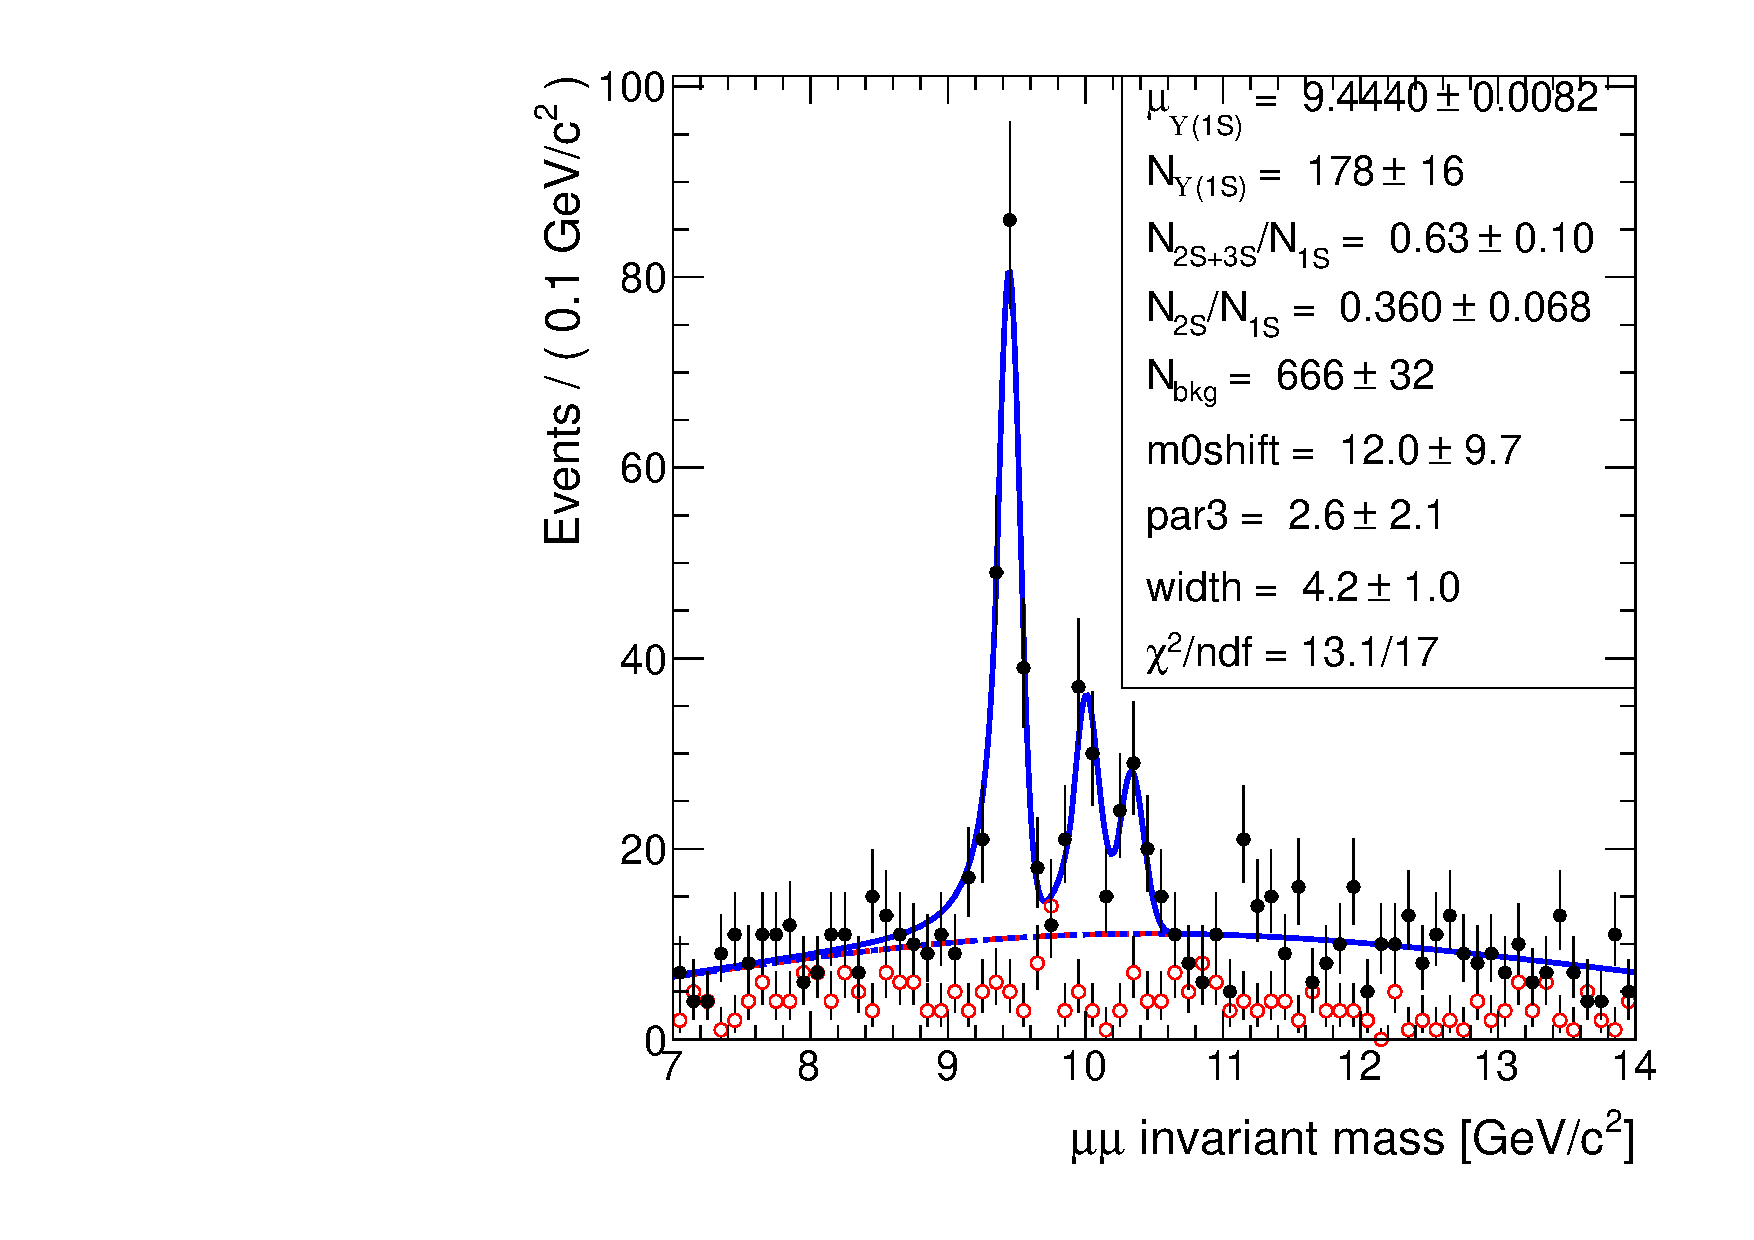
\includegraphics[angle=0,width=0.5\textwidth]{figures/pp276/masspeak_pp_HIrereco_erf_fix_paramOn_MuonPT35}\label{fig:massfits_pp_nominal_fix}} 
    \subfigure[$\pt^\mu>4.0\GeVc$; signal shape fixed to PbPb]{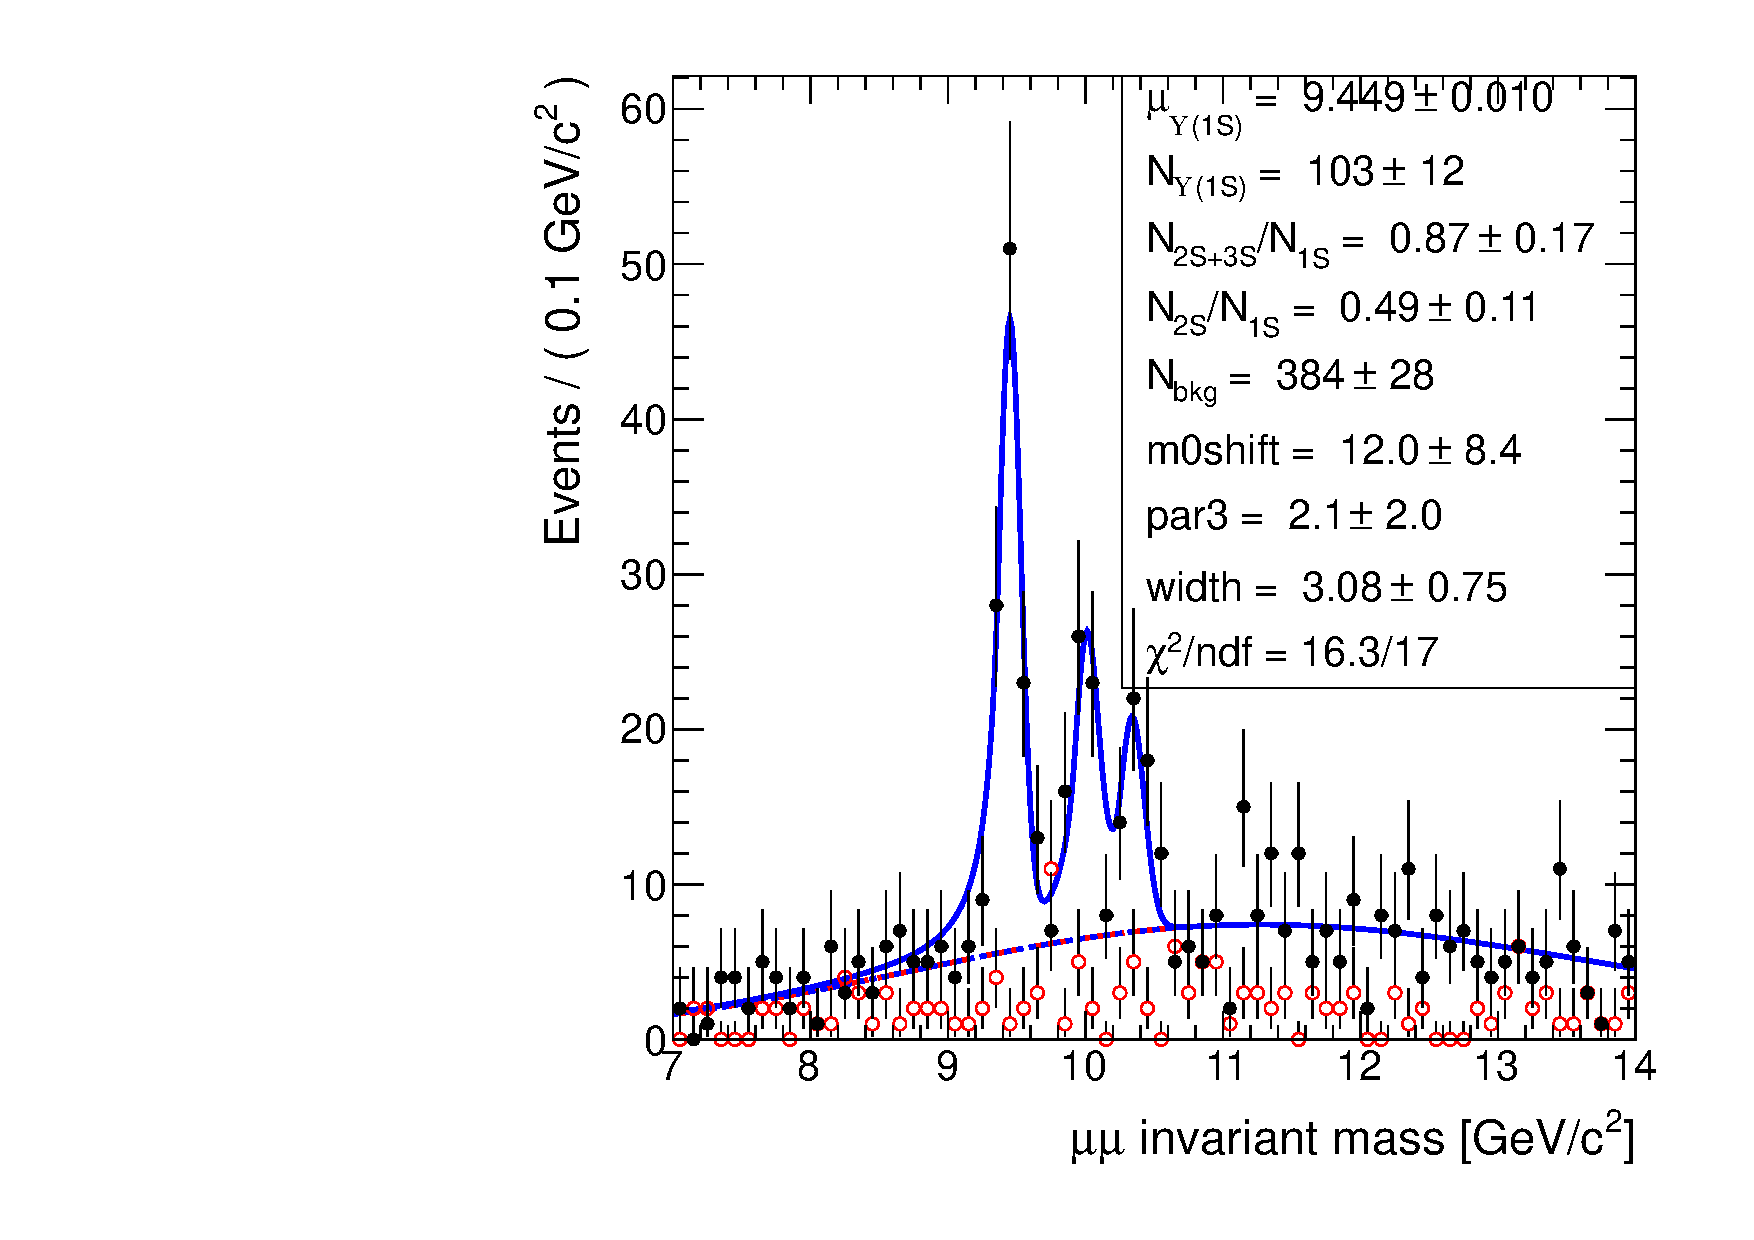
\includegraphics[angle=0,width=0.5\textwidth]{figures/pp276/masspeak_pp_HIrereco_erf_fix_paramOn}\label{fig:massfits_pp_erf_fix}}
    \caption{Mass fits to the pp data ($231 nb^{-1}$) with error function. Figs~\ref{fig:massfits_pp_nominal},~\ref{fig:massfits_pp_erf}: signal shape parameters are left floating; Figs~\ref{fig:massfits_pp_nominal_fix},~\ref{fig:massfits_pp_erf_fix}: signal shape parameters are fixed to the PbPb results.}
    \label{fig:massfits_pp_nominal_all}
  \end{center}
\end{figure}

\begin{figure}[hbtp]
  \begin{center}
    \subfigure[$\pt^\mu>3.5\GeVc$]{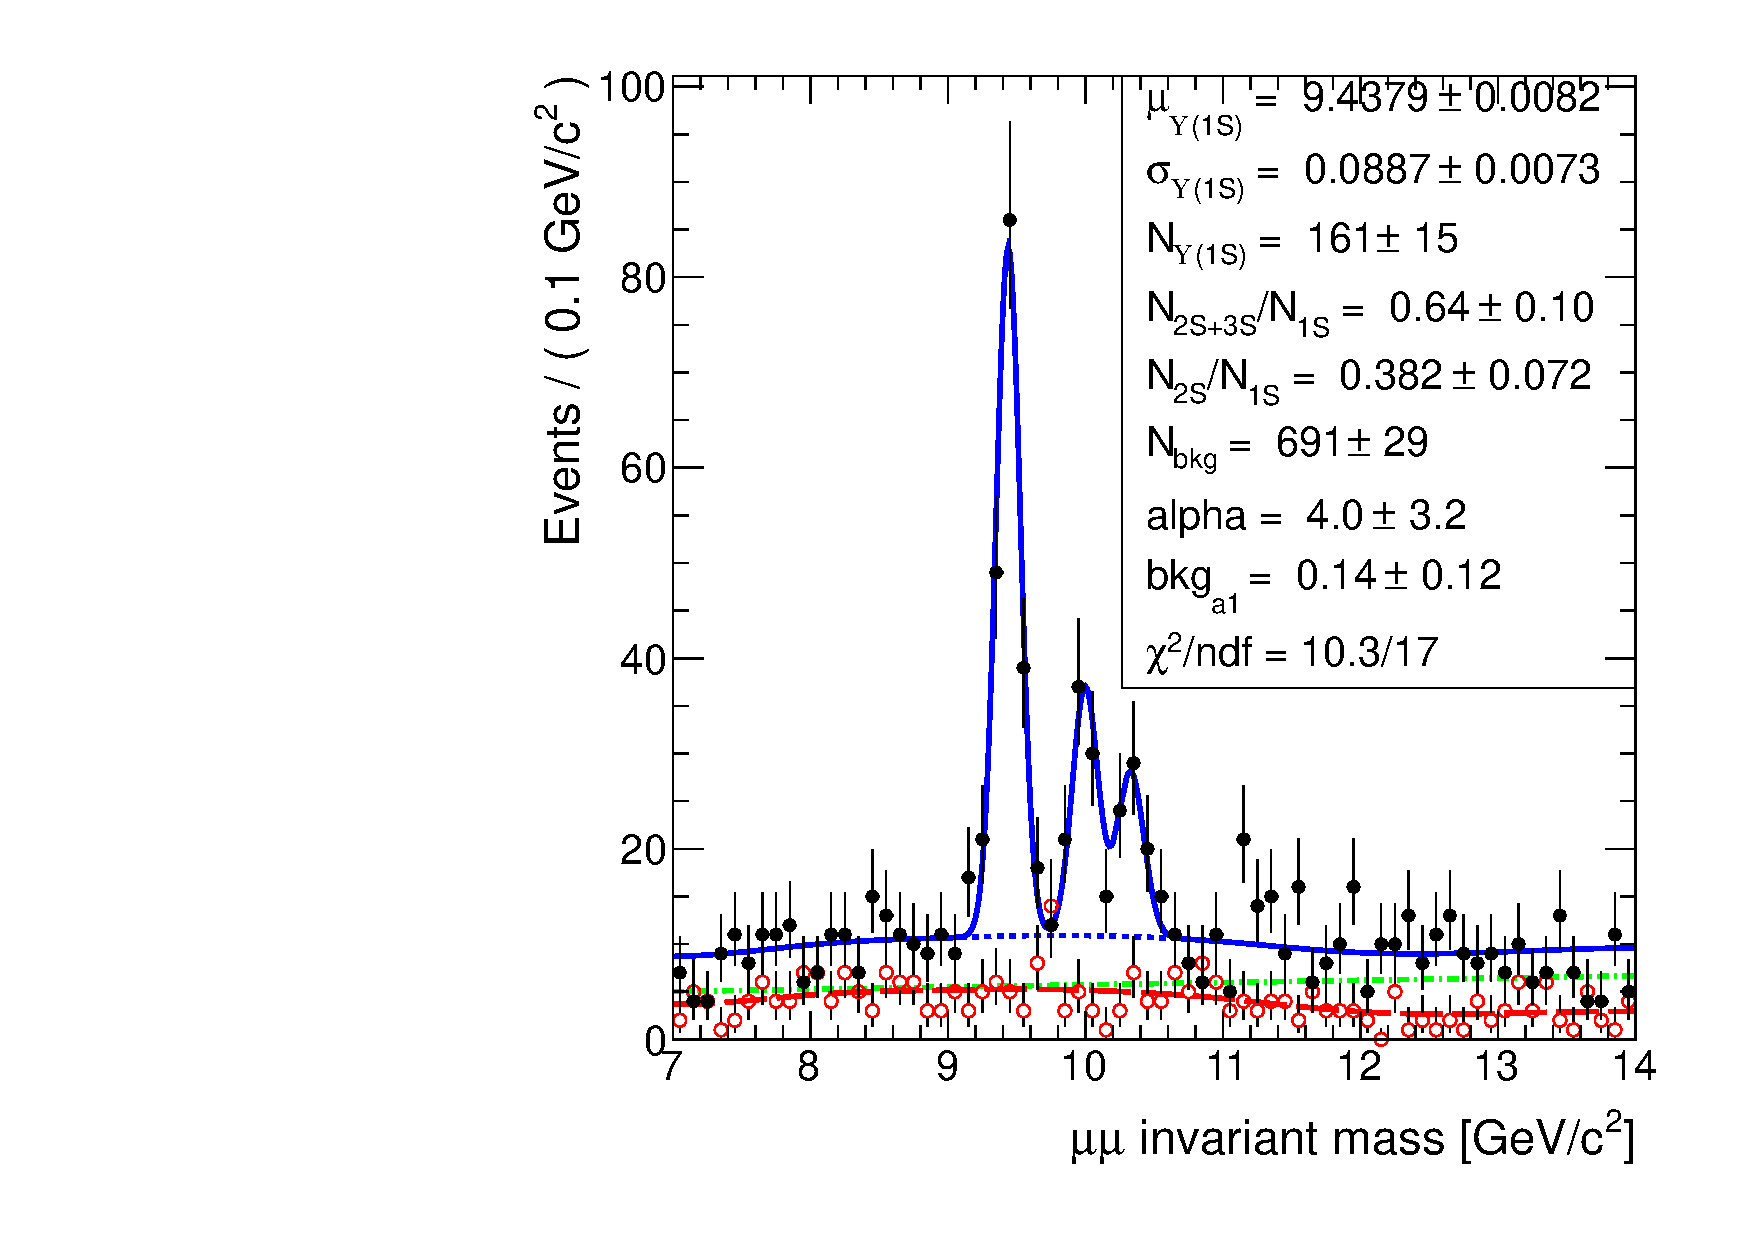
\includegraphics[angle=0,width=0.5\textwidth]{figures/pp276/masspeak_pp_HIrereco_paramOn_MuonPT35}\label{fig:massfits_pp_keys_35}}
    \subfigure[$\pt^\mu>4.0\GeVc$]{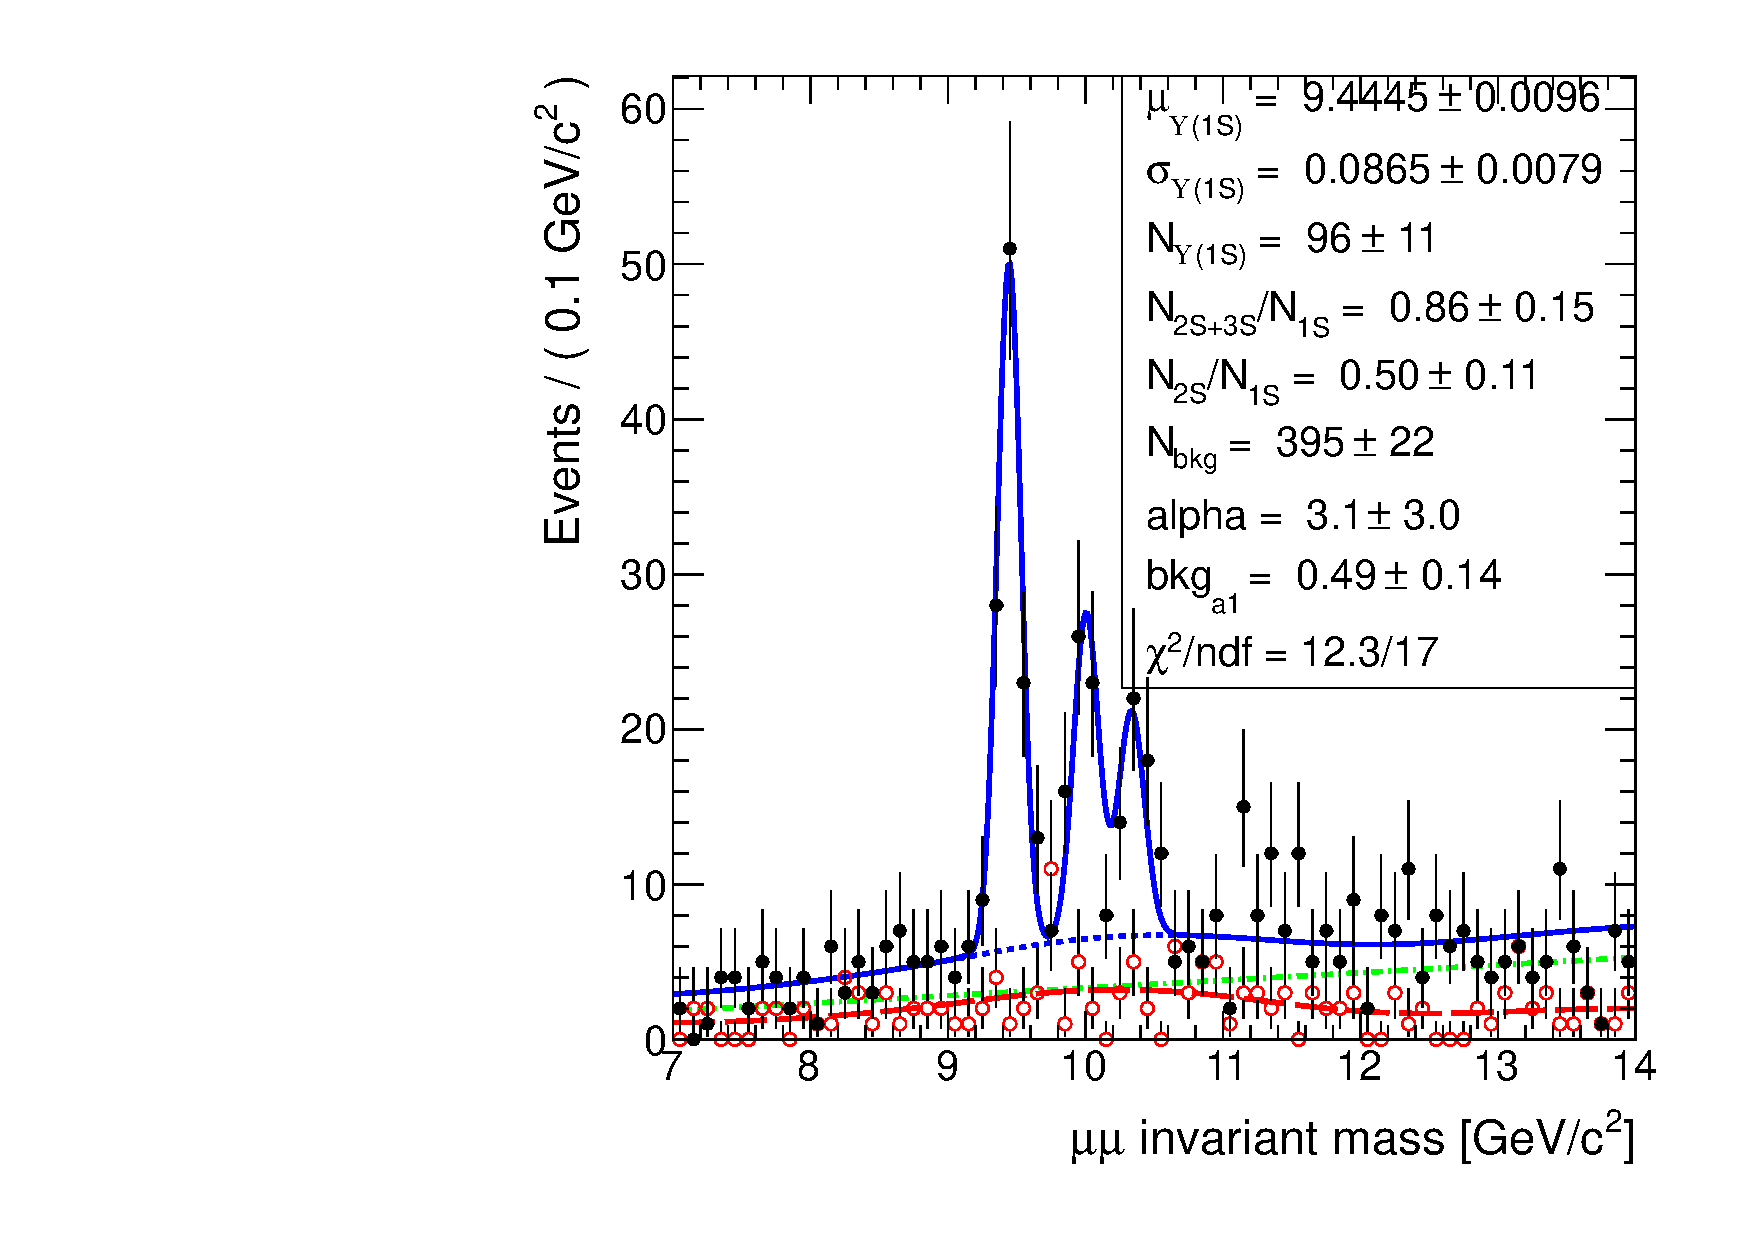
\includegraphics[angle=0,width=0.5\textwidth]{figures/pp276/masspeak_pp_HIrereco_paramOn}\label{fig:massfits_pp_keys}}\\
    \subfigure[$\pt^\mu>3.5\GeVc$; signal shape fixed to PbPb]{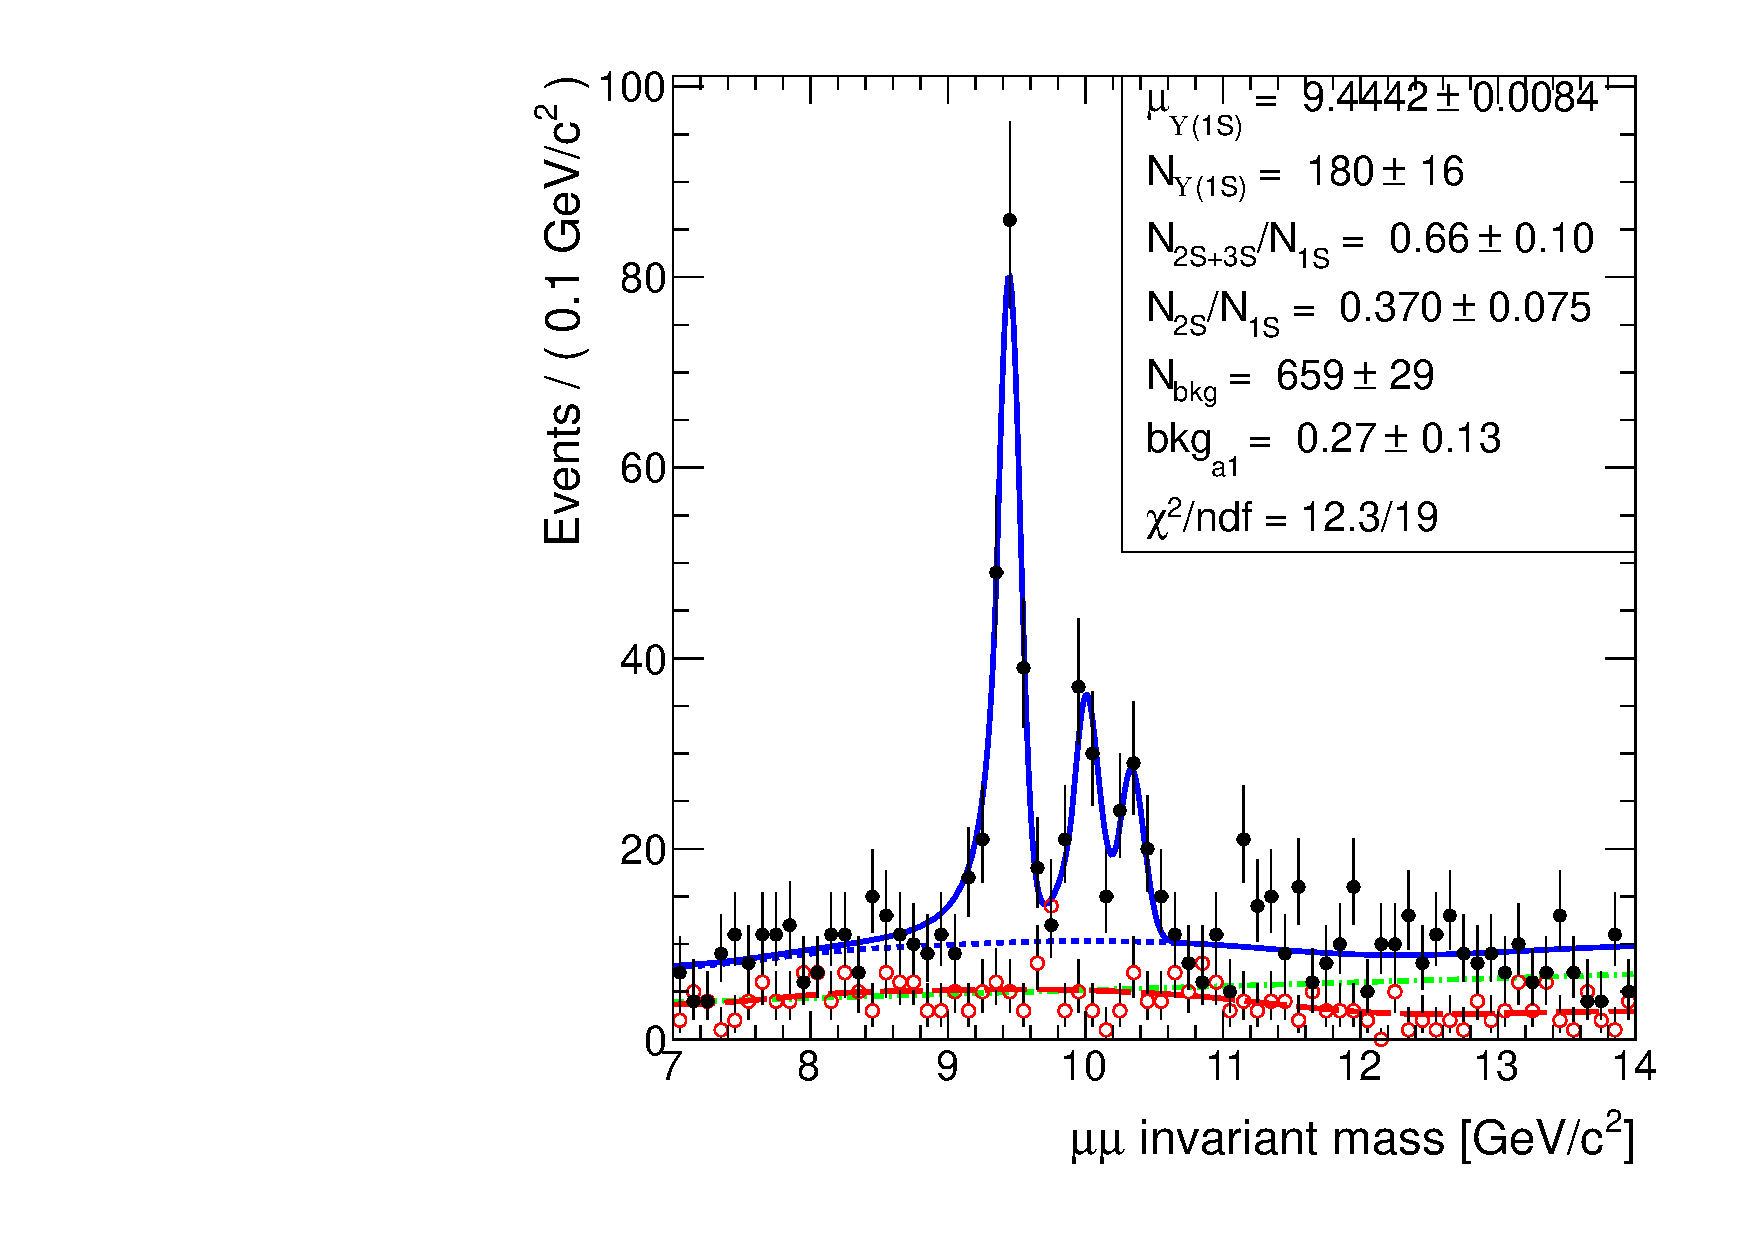
\includegraphics[angle=0,width=0.5\textwidth]{figures/pp276/masspeak_pp_HIrereco_fix_paramOn_MuonPT35}\label{fig:massfits_pp_keys_fix_35}} 
    \subfigure[$\pt^\mu>4.0\GeVc$; signal shape fixed to PbPb]{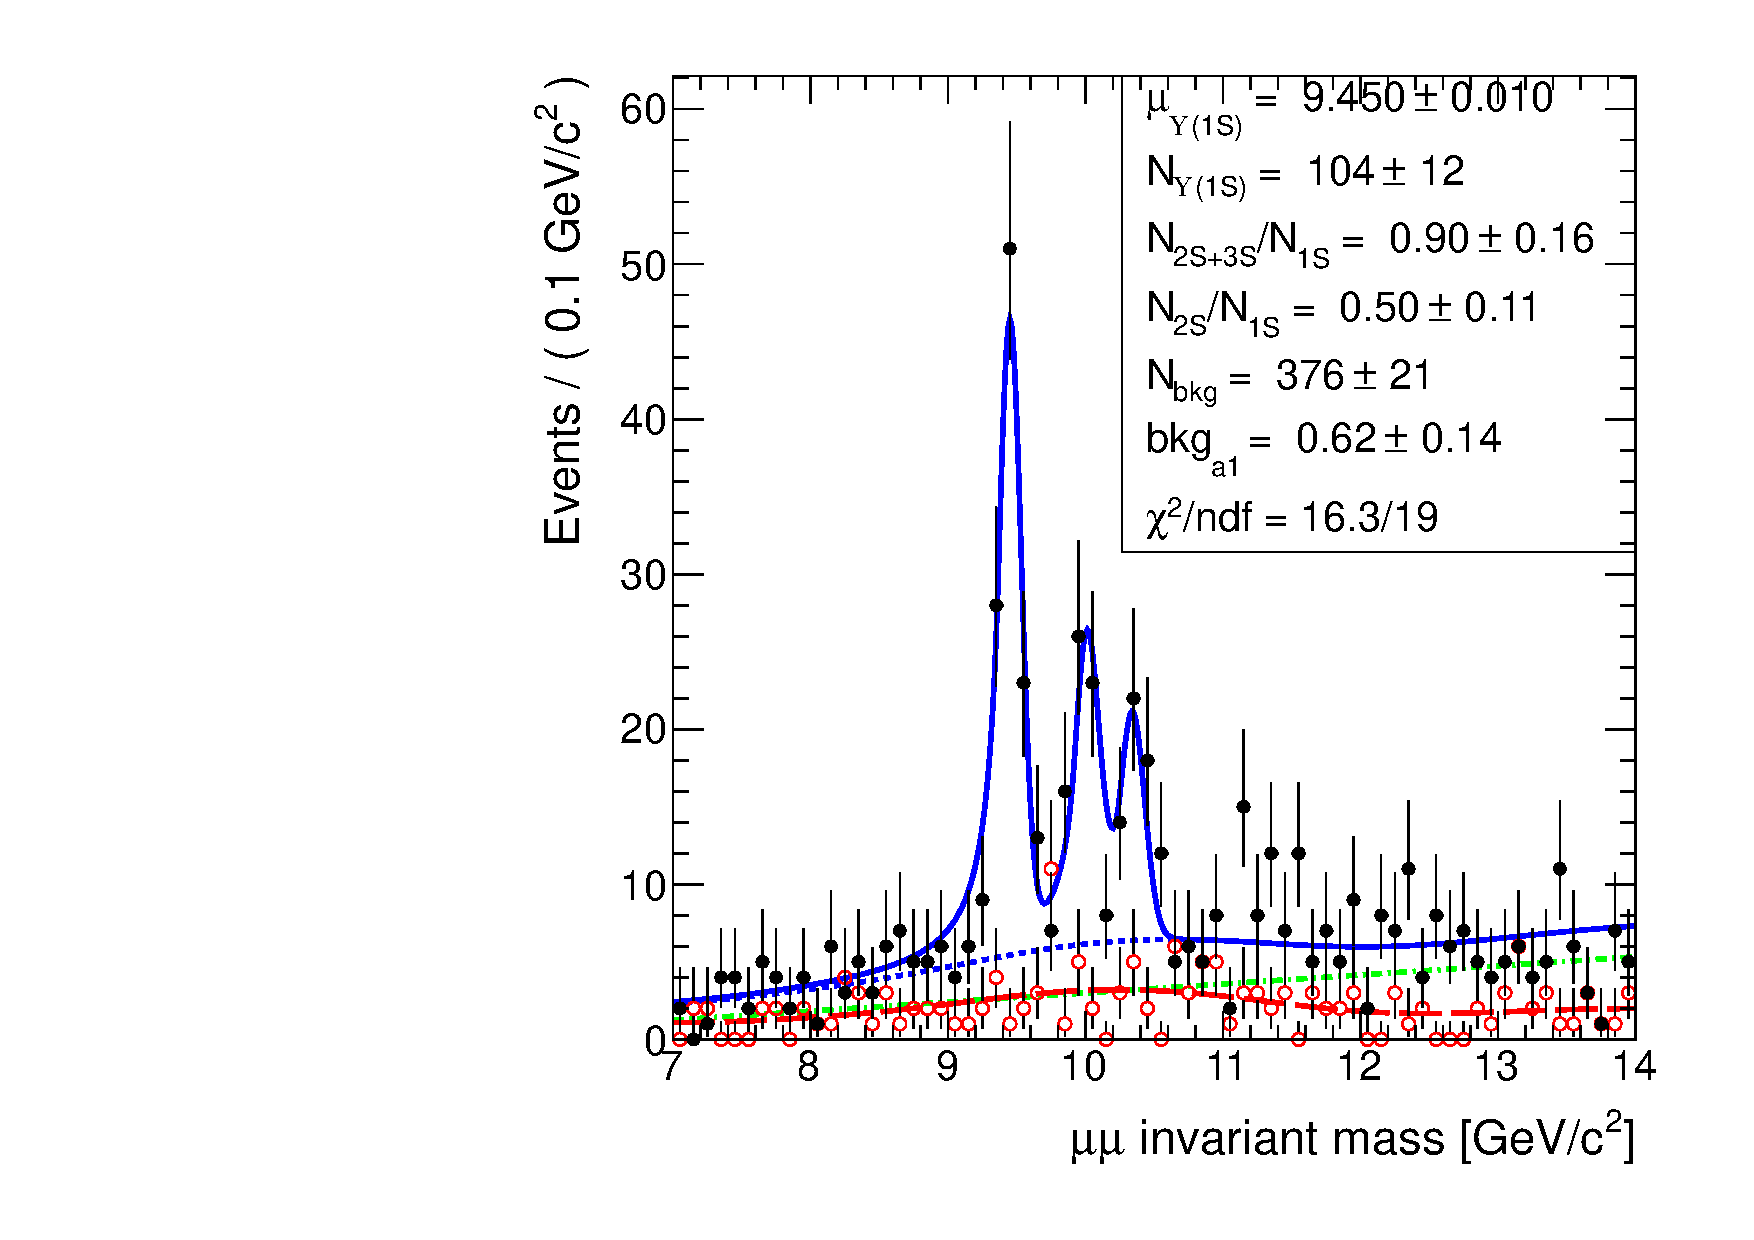
\includegraphics[angle=0,width=0.5\textwidth]{figures/pp276/masspeak_pp_HIrereco_fix_paramOn}\label{fig:massfits_pp_keys_fix}}
    \caption{Mass fits to the pp data ($231 nb^{-1}$), using like-sign information. Figs~\ref{fig:massfits_pp_keys_35},~\ref{fig:massfits_pp_keys}: signal shape parameters are left floating; Figs~\ref{fig:massfits_pp_keys_fix_35},~\ref{fig:massfits_pp_keys_fix}: signal shape parameters are fixed to the PbPb results.}
    \label{fig:massfits_pp_likesign}
  \end{center}
\end{figure}




%\subsection{Fits to the binned datasets}
%\subsubsection{Centrality dependence}
%(enter studies of mass resolution and fsr parameter dependence in MC and high-stat \JPsi data)



%\subsection{acceptance}
%\subsection{efficiency: peak counting}
%\subsection{efficiency: hit-by-hit}
%\subsection{Tag-and-probe technique}
\chapter{Efficiency}

We explore the data-driven tag and probe (T\&P) method to estimate single-muon trigger, identification, and tracking efficiencies. 
A comparison of the results obtained by applying the technique to both data and MC simulation allows to estimate related systematic uncertainties. 

The procedure is identical to that used in the previous analysis iteration, based in the 2010 \PbPb dataset, documented in Ref.~\cite{CMS_AN_2011_062}. 
The T\&P analysis is done using the official tag and probe framework, % tbd REF
as employed for example in Ref.~\cite{CMS_AN_2011_062, CMS_AN_2010-140}. 
The \Jpsi signal resonance is used to differentiate signal from background. 
Two tag-probe invariant mass distributions are formed, in the vicinity of the \Jpsi nominal mass, according to whether the probe passes or fails the criteria for which the efficiency is being measured.  
The two mass distributions are then fit simultaneously, and the efficiency $\varepsilon$ (and its uncertainty) is extracted as a common parameter in the fit, 
%
\begin{linenomath}
\begin{align}
  N_{\text{pass}} &= \varepsilon \times N_{\text{probes}} \,,\\
  N_{\text{fail}} &= (1 - \varepsilon ) \times N_{\text{probes}} \,,\nonumber
\end{align}
\end{linenomath}
%
where $N_{\text{probes}}$, $N_{\text{pass}}$, and $N_{\text{fail}}$
are the number of all probes, passing probes, and failing probes, respectively. 

Some challenges arise in measuring the tracking efficiency because in heavy ions fake and
tracking efficiency can be ``correlated'' due to the high
multiplicity, \ie one can have a fake match in events in which one has
removed the true match. 
%This problem was first encountered in the \Z
%analysis. 
Yet another problem is that measuring
the matching efficiency %($\varepsilon_{\text{M}}$) 
between a standalone muon and an inner track (necessary to promote a standalone
muon to a global muon) is not straightforward in heavy ions~\cite{CMS_AN_2011_062}. 
Furthermore, to fit failing tag and probe pairs becomes challenging due to the poor
resolution of the standalone (STA) muons.
%
%To measure the standalone muon to inner track matching
%efficiency, one could try to use as probes standalone muons and
%define passing probes as probes that are also global muons. 
%%
%But then one can get failing probes due to the following reasons:
%\begin{enumerate}
%\item The probe was a true muon with an outer track and an inner track
%  but failed the global matching criteria (that is a loss due to the
%  true matching efficiency which you want to measure)
%\item The probe was a true muon but the
%  inner track was a fake match. This could happen due to the very high inner tracker occupancy combined with tracking inefficiency. Then one would expect in most cases this
%  probe not to be a global muon, due to the tighter matching criteria.
%\item The probe was a fake muon, but the inner track part was a true muon. This is probably highly unlikely due to
%  the lower occupancy in the muon chambers, but possible.
%\item The probe was a fake muon, as well as the
%  inner track part. It could still survive the global muon criteria,
%  but independent of that, it is not a muon from the resonance decay
%  that is used for the Tag and Probe.
%\end{enumerate}
%
%If one uses the standalone momentum measurement, cases 1. and 2. will
%end up in the \Jpsi peak of the failing probe distribution, while 3. and 4. would just
%contribute to the background continuum. But case 2. is not failing
%because of the matching efficiency, but because of the tracking
%efficiency. So in this case, one would not measure $(1 -
%\varepsilon_{\text{M}})$ with the failing probes.
%
%If, however one uses the inner track momentum measurement, case
%2. would not end up in the peak of the failing probe distribution, as
%the track was a fake track. Instead, now case 3. would end up in the
%peak of the failing probes. Again, one would not measure directly $(1
%- \varepsilon_{\text{M}})$ with the failing probes, even though it might be
%much closer to the correct value, as case 3. is much less likely than
%case 2..
%
%One could completely ignore the failing probes and only fit the
%passing probes, but then one is left with the problem of not knowing
%the uncertainty on the efficiency: one cannot use binomial statistics
%due to the background.
%
In general, %instead, 
we will compare the efficiency estimations found with T\&P in Monte Carlo simulation and  data as a cross check of the Monte Carlo based efficiency corrections. 

Tags are selected as high quality, global muons, which are matched to the single muon trigger path HLT\_HIL1SingleMu0\_HighQ,  
%Tags are selected as muons which are matched to either the HLT\_HIL1DoubleMu0\_HighQ or the HLT\_HIL2DoubleMu3 trigger (our two triggers with the lowest \pt thresholds)
that also pass the offline muon selection used in the data analysis.
% and that are within the single muon acceptance.
%
These tag muons are combined with probe muons to form tag-probe
pairs. The probe muon selection depends on the efficiency being measured.
A condition is applied to the probes which are split into the passing and failing probe categories. 
It is the efficiency of this condition relative to all probes that is measured with T\&P.
%
We have used the following three probe categories to measure the inner-track reconstruction,
muon reconstruction and identification, and muon trigger efficiencies:
%
\begin{itemize}
\item inner-track reconstruction efficiency (including inner to
  outer track matching, and track quality criteria): %and the quality cuts as those are inner track selections:
  \begin{itemize}
  \item probe: a standalone muon (the four-momentum information is taken from the
    standalone part exclusively)
  \item passing probe: probe that is also a global muon passing the quality cuts
  \end{itemize}
\item global muon reconstruction and identification efficiency (relative to tracker muon)
%(including the  inner to outer track matching efficiency):
  \begin{itemize}
  \item probe: tracker muon %inner track of type \verb=hiSelectedTrack=   whithin the acceptance
  \item passing probe: probe that can be matched to a global muon and that fulfills the analysis muon selection criteria
  \end{itemize}
\item trigger efficiency:
  \begin{itemize}
  \item probe: (global) muon that satisfies the offline analysis selection criteria
%global muon that fulfills all quality cuts in the acceptance
    \item passing probe: probe that can be matched to (one leg of) HLT\_HIL1DoubleMu0\_HighQ trigger path.
  \end{itemize}
\end{itemize}

In order to attempt a reduction of the background level, further selection criteria have been tried. 
%For example, when evaluating efficiencies other than trigger, matching HLT\_HIL1DoubleMu0\_HighQ is applied.
A requirement on the dimuon $\pt > 6.5 \GeVc$ is applied and as well as a single muon  $\pt > 4.0 \GeVc$
In all cases, identical selection criteria are applied to both data and simulation: this is necessary for yielding reliable systematic estimates based on data-MC efficiency results comparison. 

The efficiency in simulation is measured using T\&P on a prompt \Jpsi sample.  
The MC sample is weighted for the centrality dependence (which scales with \ncoll) and for the relative weights between the different \pt bins used in the sample production. 
% as listed in \tab{tab:wfilter}. 
While the T\&P framework allows for weighted samples, the uncertainty estimates using the current version of RooFit for weighted datasets is not accurate. 
%properly taking into account the weighted errors when calculating the error on the fit result. 
However, employing large MC statistics, we will take the size of the corresponding errors to be negligible. 
%Therefore the error bars on the MC Tag and Probe efficiencies are not plotted. However, as we have a lot of MC statistics, we could estimate the size of the errors to be negligible. Figure~\ref{fig:tnpTrkErr} illustrate the small size of the error for one \pt bin of the \Jpsi simulation in 6-9GeV/c in bin of \Jpsi \pt, not weighted. It is 2\% of 84\% for that bin.

The estimation of the systematic uncertainty will be assigned by comparing results between data and simulation.  
%Currently, only the results extracted from data are provided; the T\&P MC results are still being finalized.  
%Systematic uncertainty can be estimated once we get the efficiencies in MC.
%
We also note that only results above the single-muon \pt of 4.0\GeVc are within the acceptance used in the analysis. 
This tends to reach the muon efficiency plateau, and is less affected by systematics related to the detailed description of the efficiency turn-on. 


%TBD: describe the fit model!!!!!

\subsubsection{Trigger efficiency}

The trigger efficiency is, in general, the easiest one to fit for, given the cleaner probe sample. The signal shape is describe by a Crystal Ball plus a Gaussian. The addition of the Gaussian is motivated to describe varying detector resolution. The parameters in the Crystal Ball as well as the width of the Gaussian are free parameters of the fit. The background is described by an exponential function. 
%In the MC case, we proceed similarly using a Crystal Ball plus a Gaussian for the signal and an exponential background.  

Figure~\ref{fig:tnpTrigFit} shows fits to the passing and failing samples of T\&P pairs for the
trigger efficiency measurement, using the integrated data and MC samples. % in data, respectively. 
%TBD: add MB integrated fits in data and MC
%
%The \pt and $\eta$ dependence of the trigger efficiency  compares rather well between 2011 and 2010 and is shown in  \fig{fig:tnpTrigEff} left column for \Jpsi \pt$> 6.5$~Gev/c. 
%
%The \pt and $\eta$ integrated trigger  efficiency is $92.6\pm0.6$\%  for the HLT\_HIL1DoubleMu0\_HighQ % and $78.4\pm0.7$\%  forHLT\_HIL2DoubleMu3 
%in the 2011 data. 
Figure~\ref{fig:tnpTrigEff} shows the trigger efficiency measured as a function of probe \pt and pseudo-rapidity.
Also shown is the trigger efficiency as function of centrality which, as expected, shows no significant dependence. 
A reasonable agreement between data and simulation is obtained especially in the most peripheral bins. 


\begin{figure}[hp]
  \begin{center}
    \subfigure[Data]{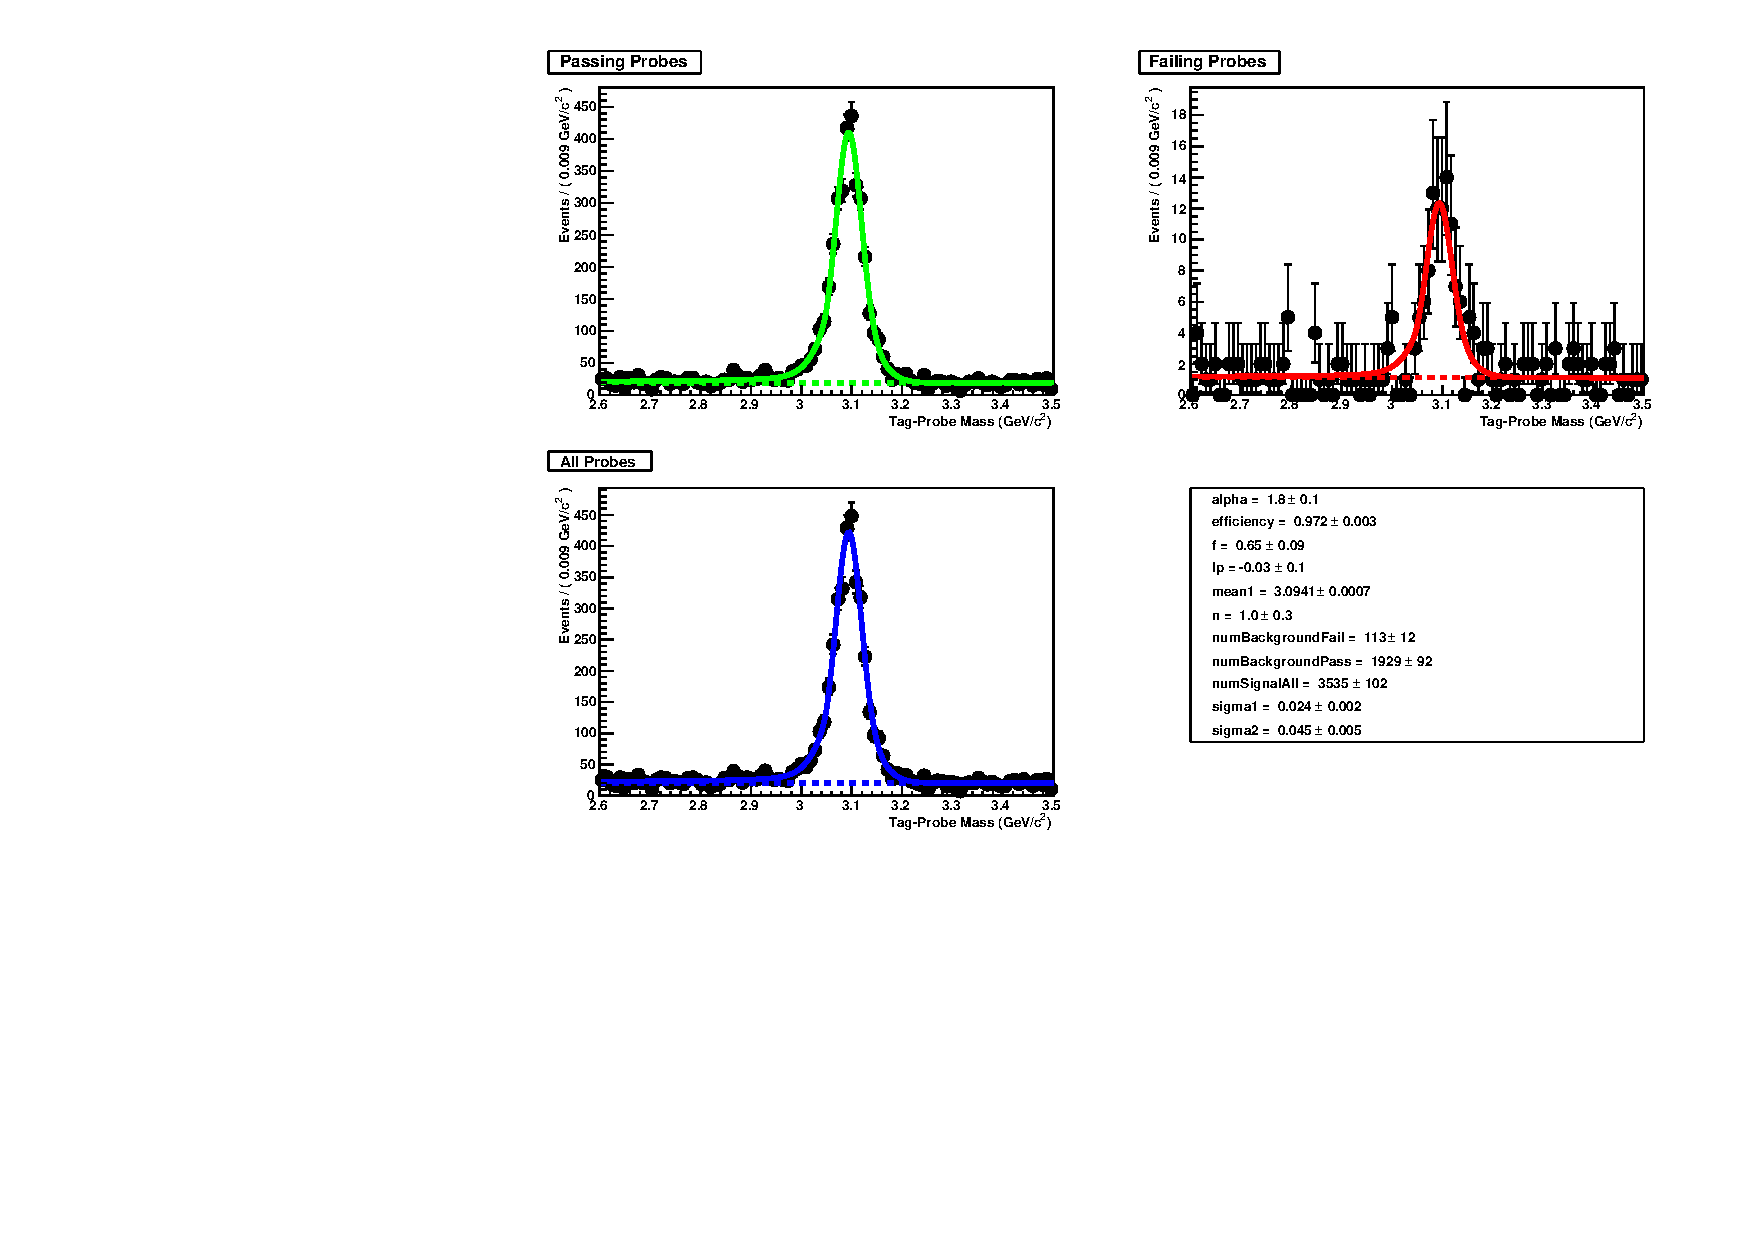
\includegraphics[width=0.9\textwidth]{figures/efficiency/RD_Trg_massfit_0100_HLTL1}}\hspace{1em}
    \subfigure[Monte Carlo]{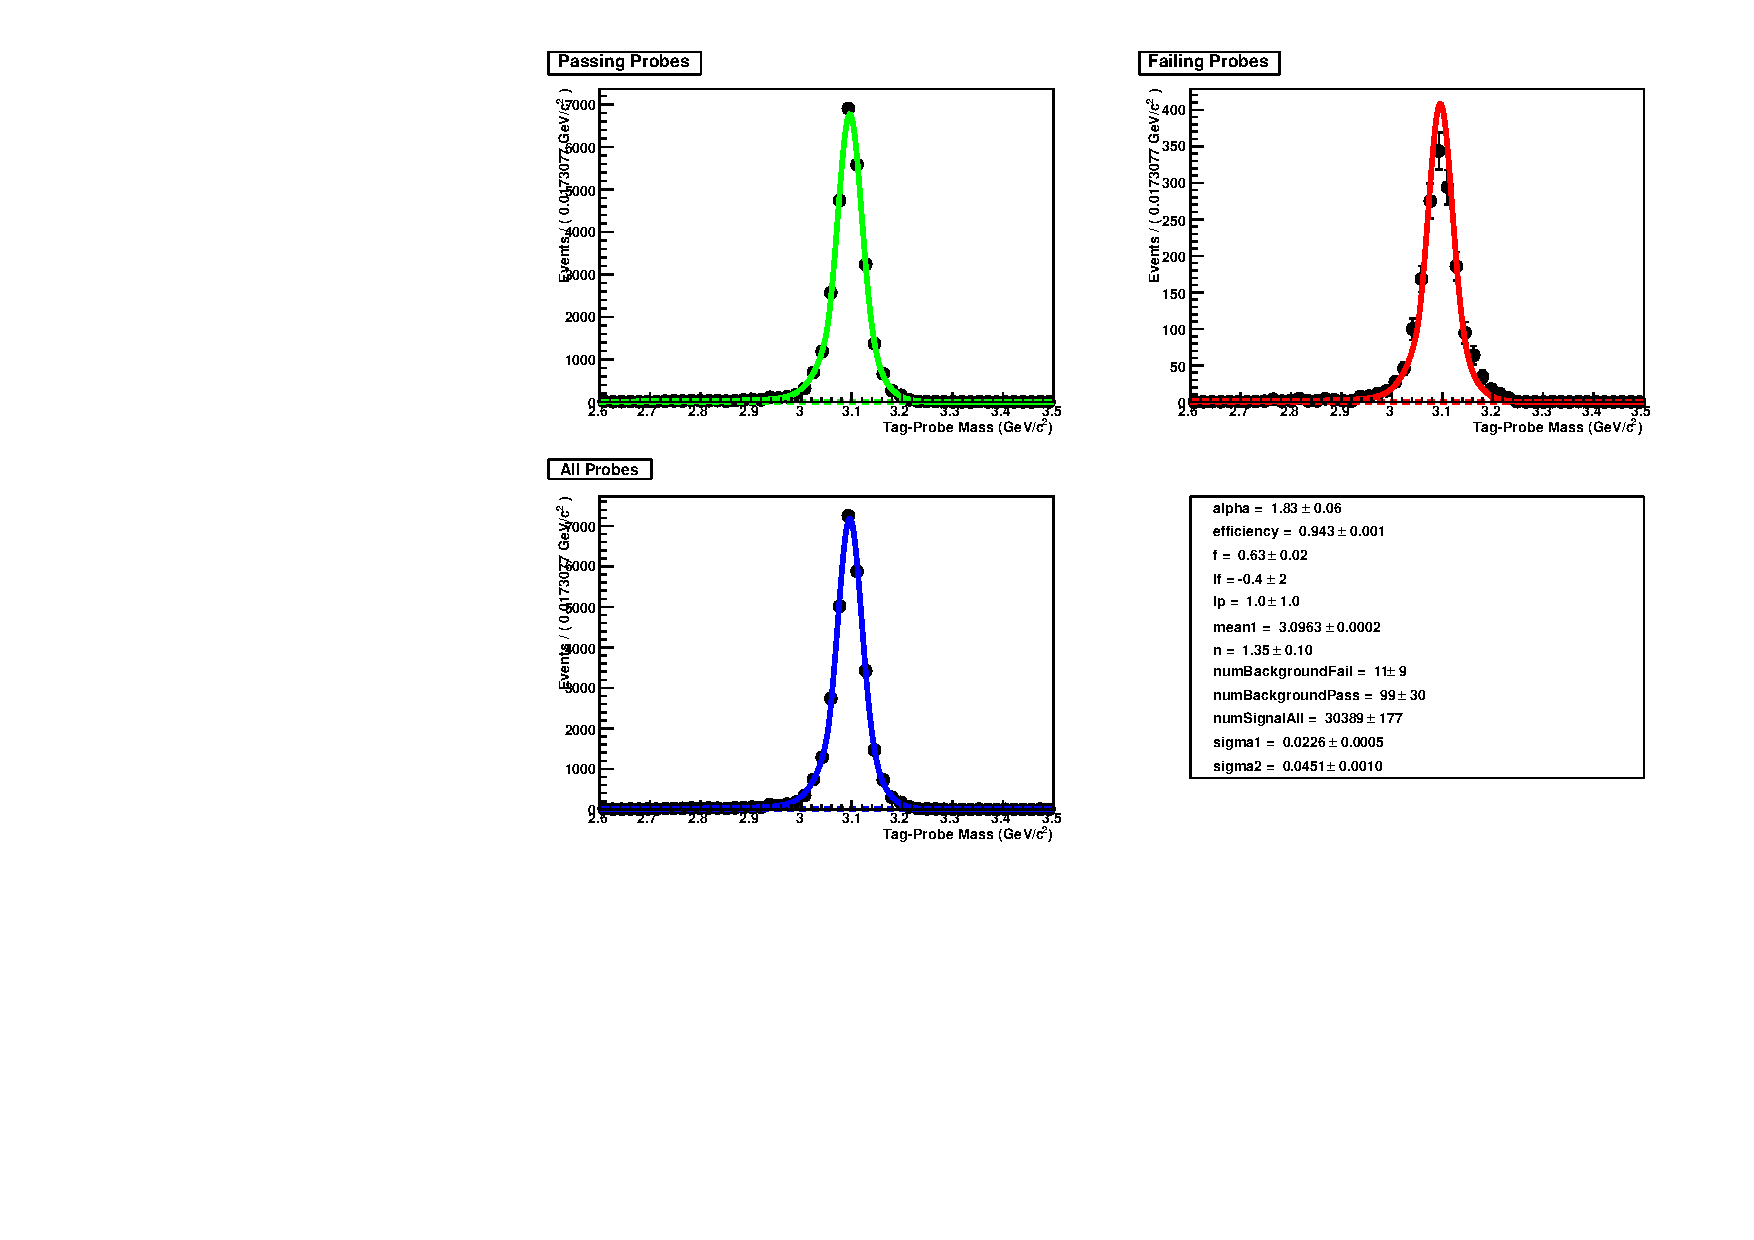
\includegraphics[width=0.9\textwidth]{figures/efficiency/MC_Trg_massfit_0100_HLTL1}}
    \caption{Examples of tag-probe pair mass fits used to extract the trigger efficiency for data and MC.}%TBD add MB inetagretyd plot in data and MC!
    \label{fig:tnpTrigFit}
  \end{center}
\end{figure}


\begin{figure}[hp]
  \begin{center}
    \subfigure[Trigger efficiency dependence on muon $\pt$.]{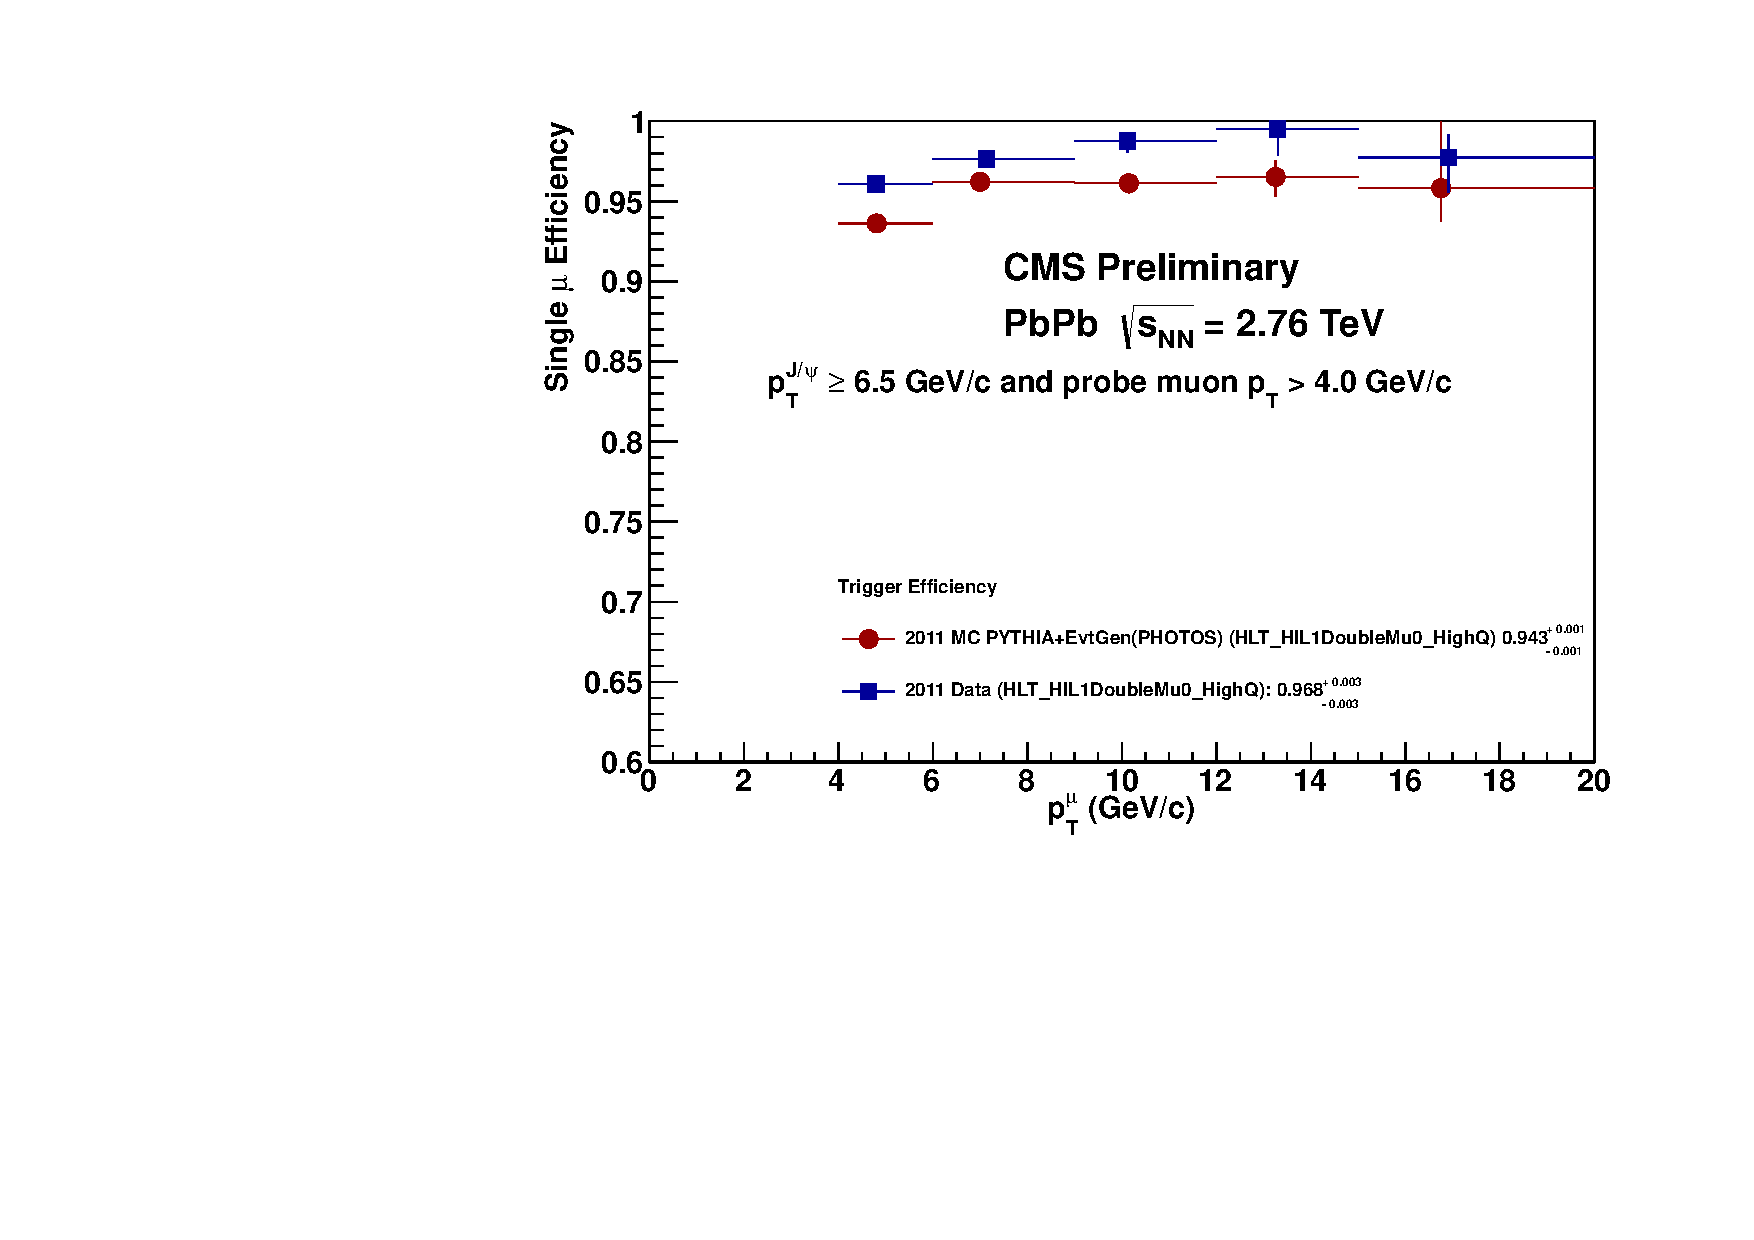
\includegraphics[width=0.6\textwidth]{figures/efficiency/Trg_Comp_HI_pt_RD_MC_HighPt_notriggermatched}}  \\ %\hspace{1em}
    \subfigure[Trigger efficiency dependence on muon $\eta$.]{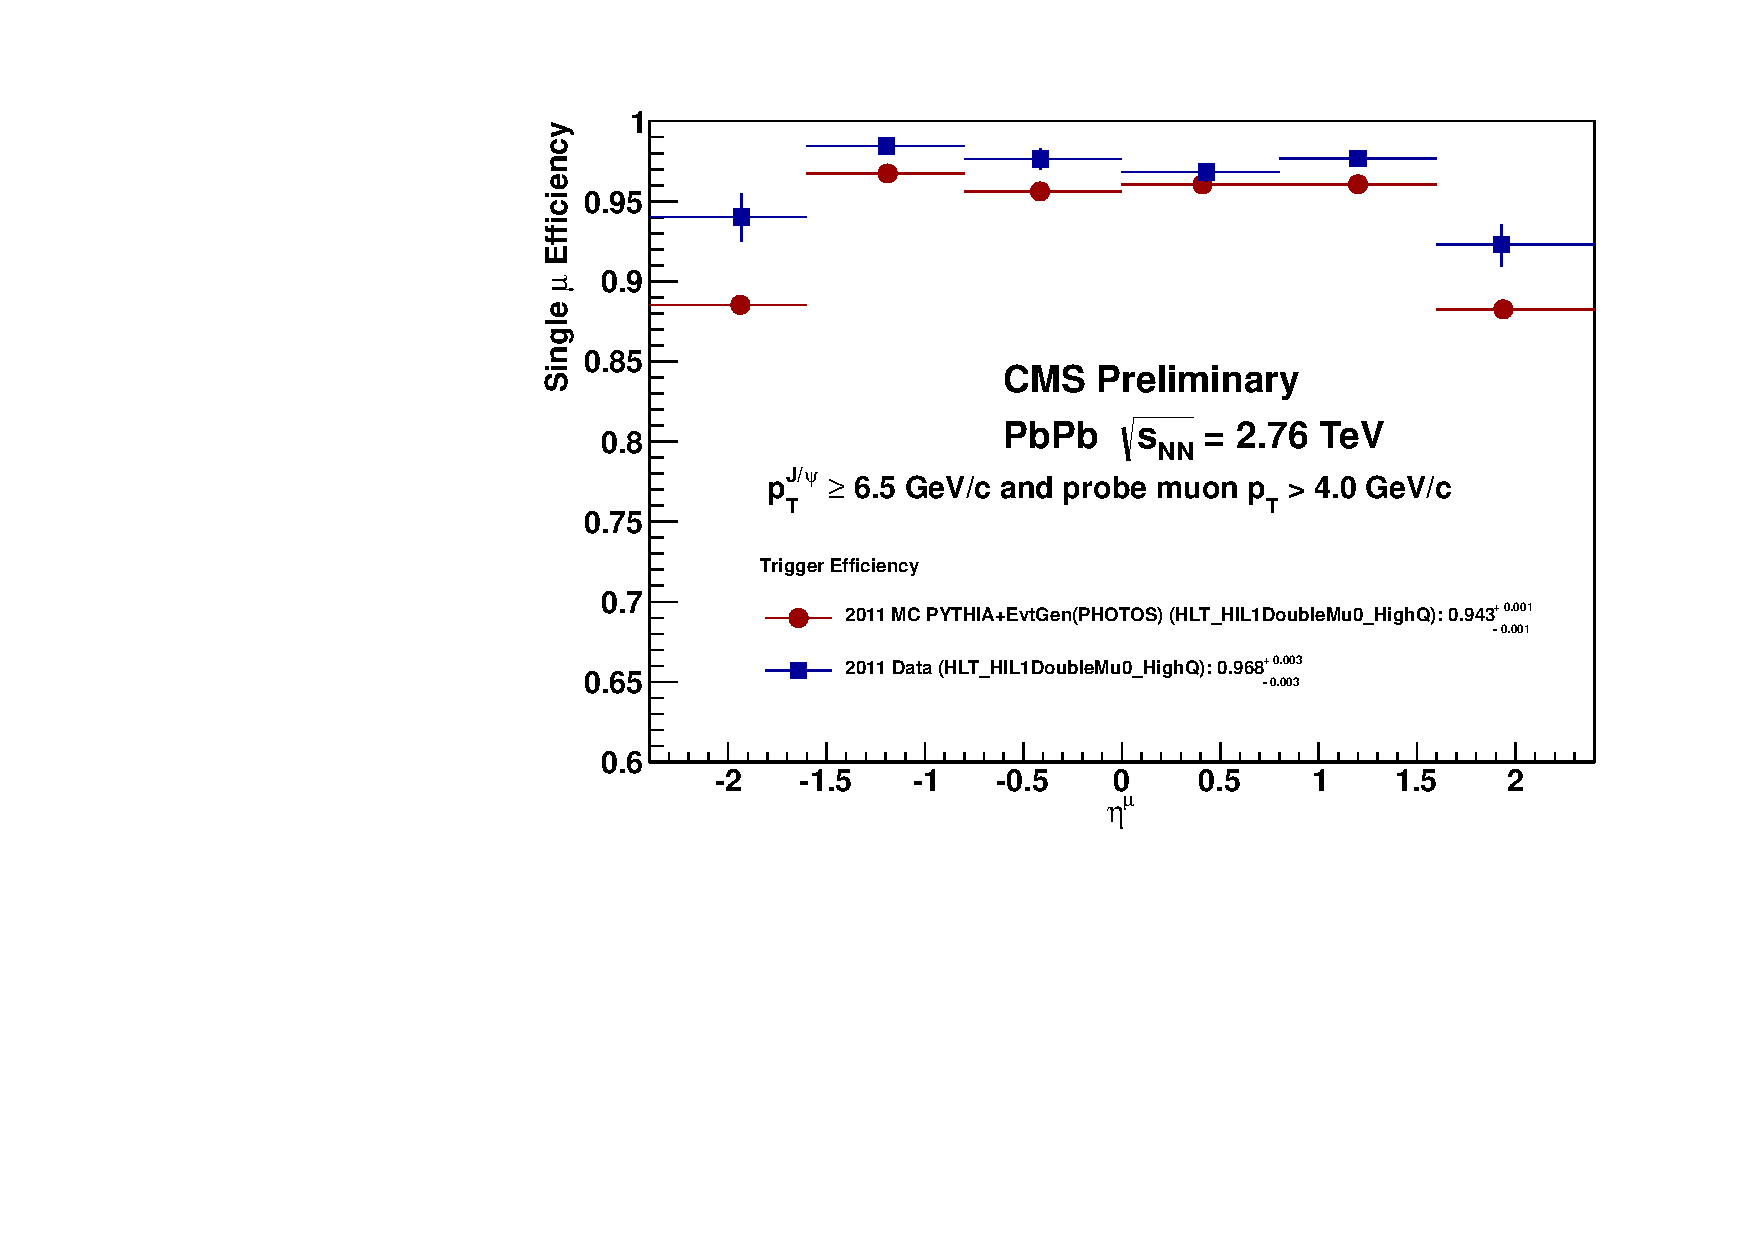
\includegraphics[width=0.6\textwidth]{figures/efficiency/Trg_Comp_HI_eta_RD_MC_HighPt_notriggermatched}} \\
    \subfigure[Trigger efficiency dependence on event centrality.]{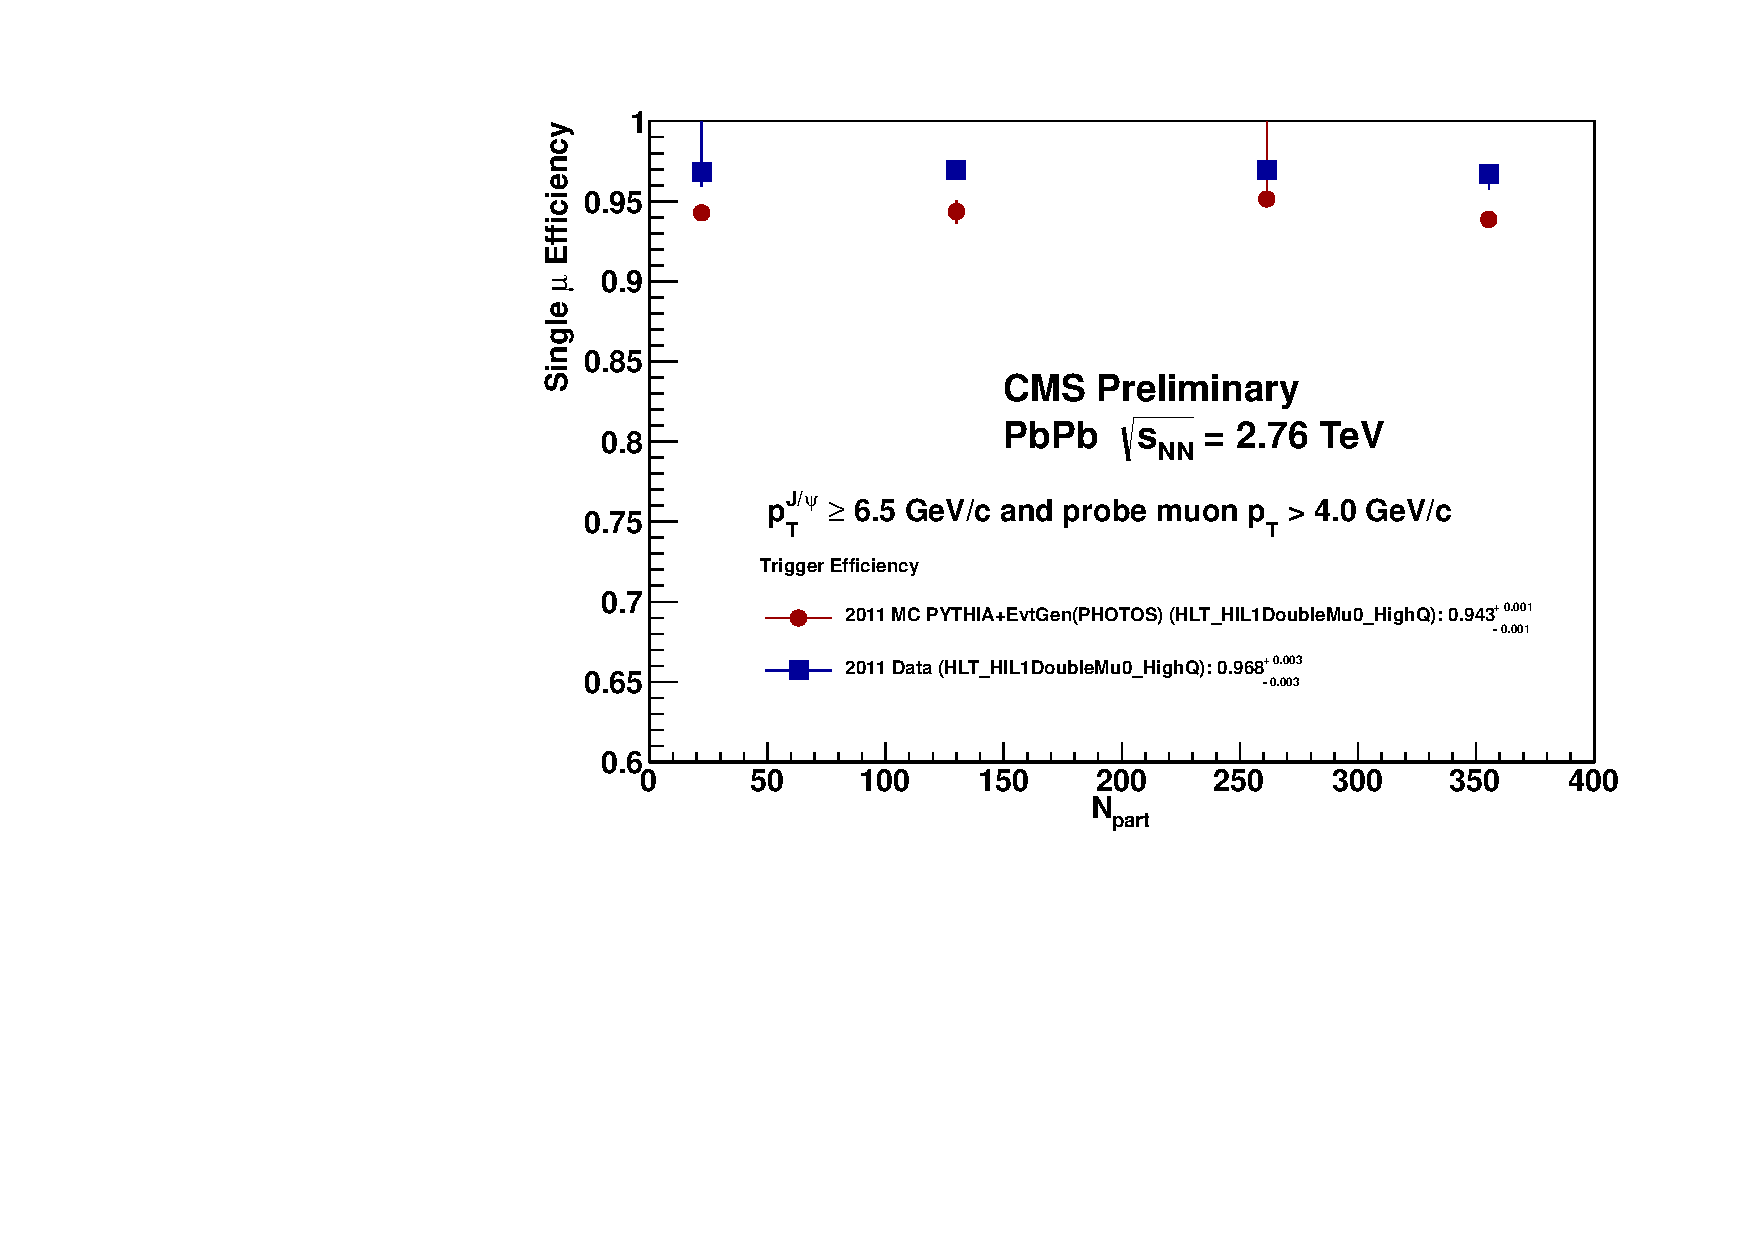
\includegraphics[width=0.6\textwidth]{figures/efficiency/Trg_Comp_HI_CNT_RD_MC_HighPt_notriggermatched}}
    \caption{Trigger efficiency measurements with tag and probe, and dependencies on probe muon \pt and pseudo-rapidity and event centrality. 
The efficiencies measured in the full samples are represented as open symbols and the corresponding numerical values are displayed for data and simulation. %TBD add MB/integrated point!
}
    \label{fig:tnpTrigEff}
  \end{center}
\end{figure}


%\subsubsection{Muon identification efficiency}

%In \fig{fig:tnpTrkFit} we show a good and a poor example of the fits to the passing and failing sample of tag and probe pairs for the muon identification efficiency measurement in data and MC, respectively. As noted above this includes the inner to outer track matching efficiency. Because standalone muons are used as probes, the momentum measured in the muon station has to be used in order not to have a different mass resolution in passing and failing probes (failing probes have no inner track matched, and thus no momentum measured with the inner tracker). This leads to a worse mass resolution than in the other two tag and probe pair mass distributions and a single Gaussian is used as signal pdf.

%Due to the poor momentum resolution also here we are subject to fluctuations and the \pt and $\eta$ dependence of the muon ID efficiency compares not so well between data and MC as shown in \fig{fig:tnpTrigEff}. The efficiency in data shows a \pt dependence not seen in MC, but it is unclear how significant this effect is due to the unknonw error on the MC. The agreement at high \pt is rather good. The tracking efficiency in data as function of $\eta$ is consistently lower than in MC. The \pt and $\eta$ integrated trigger efficiency is 89.2\,\% in MC and $78.8^{+8.8}_{-5.7}$\,\%. Half the difference is taken as a systematic uncertainty on the MC based efficiency correction. From the three efficiency comparisons between data and MC, this one has the largest systematic uncertainty. Adding all in quadrature gives a 6.7\,\% uncertainty on the single muon efficiency due to the data to MC comparison, which is a 13.4\,\% uncertainty on the \mumu pair efficiency.


\subsubsection{Muon identification efficiency}

%As for the trigger case, 
%Following the same idea as with the trigger efficiency 
We fit simultaneously the passing and failing tag-probe pairs mass distribution using a Crystal Ball function and (when needed to account for different resolutions) a Gaussian.
% to account for varying detector resolution. This time however a simple 
A first order polynomial is used to describe the background. For the MC case, a  Crystal Ball and an exponential describe the signal and background shapes. 

 T\&P mass fits for the muon identification efficiency are shown in \fig{fig:tnpMuIDFit}, for the integrated data and MC samples. 
These illustrate the considerably high level of background involved, in the heavy-ion environment. 
%The fits for all the centrality bins were well described with the previous choice of pdfs. 
%
Figure~\ref{fig:tnpMuIDEff} shows the muon identification efficiency measured as a function of probe \pt and pseudo-rapidity, and event centrality. 
A good agreement between data and simulation is observed. 
%The systematic is 0.4\%.
%we notice an improvement of the muon identification efficiency with respects to last year's results. This is due to the fact that this year we are using tracker muons as probes as opposed to \verb=hiGlobalPrimTrack=. Again no centrality dependency is observed.

\begin{figure}[hp]
  \begin{center}
    \subfigure[Data]{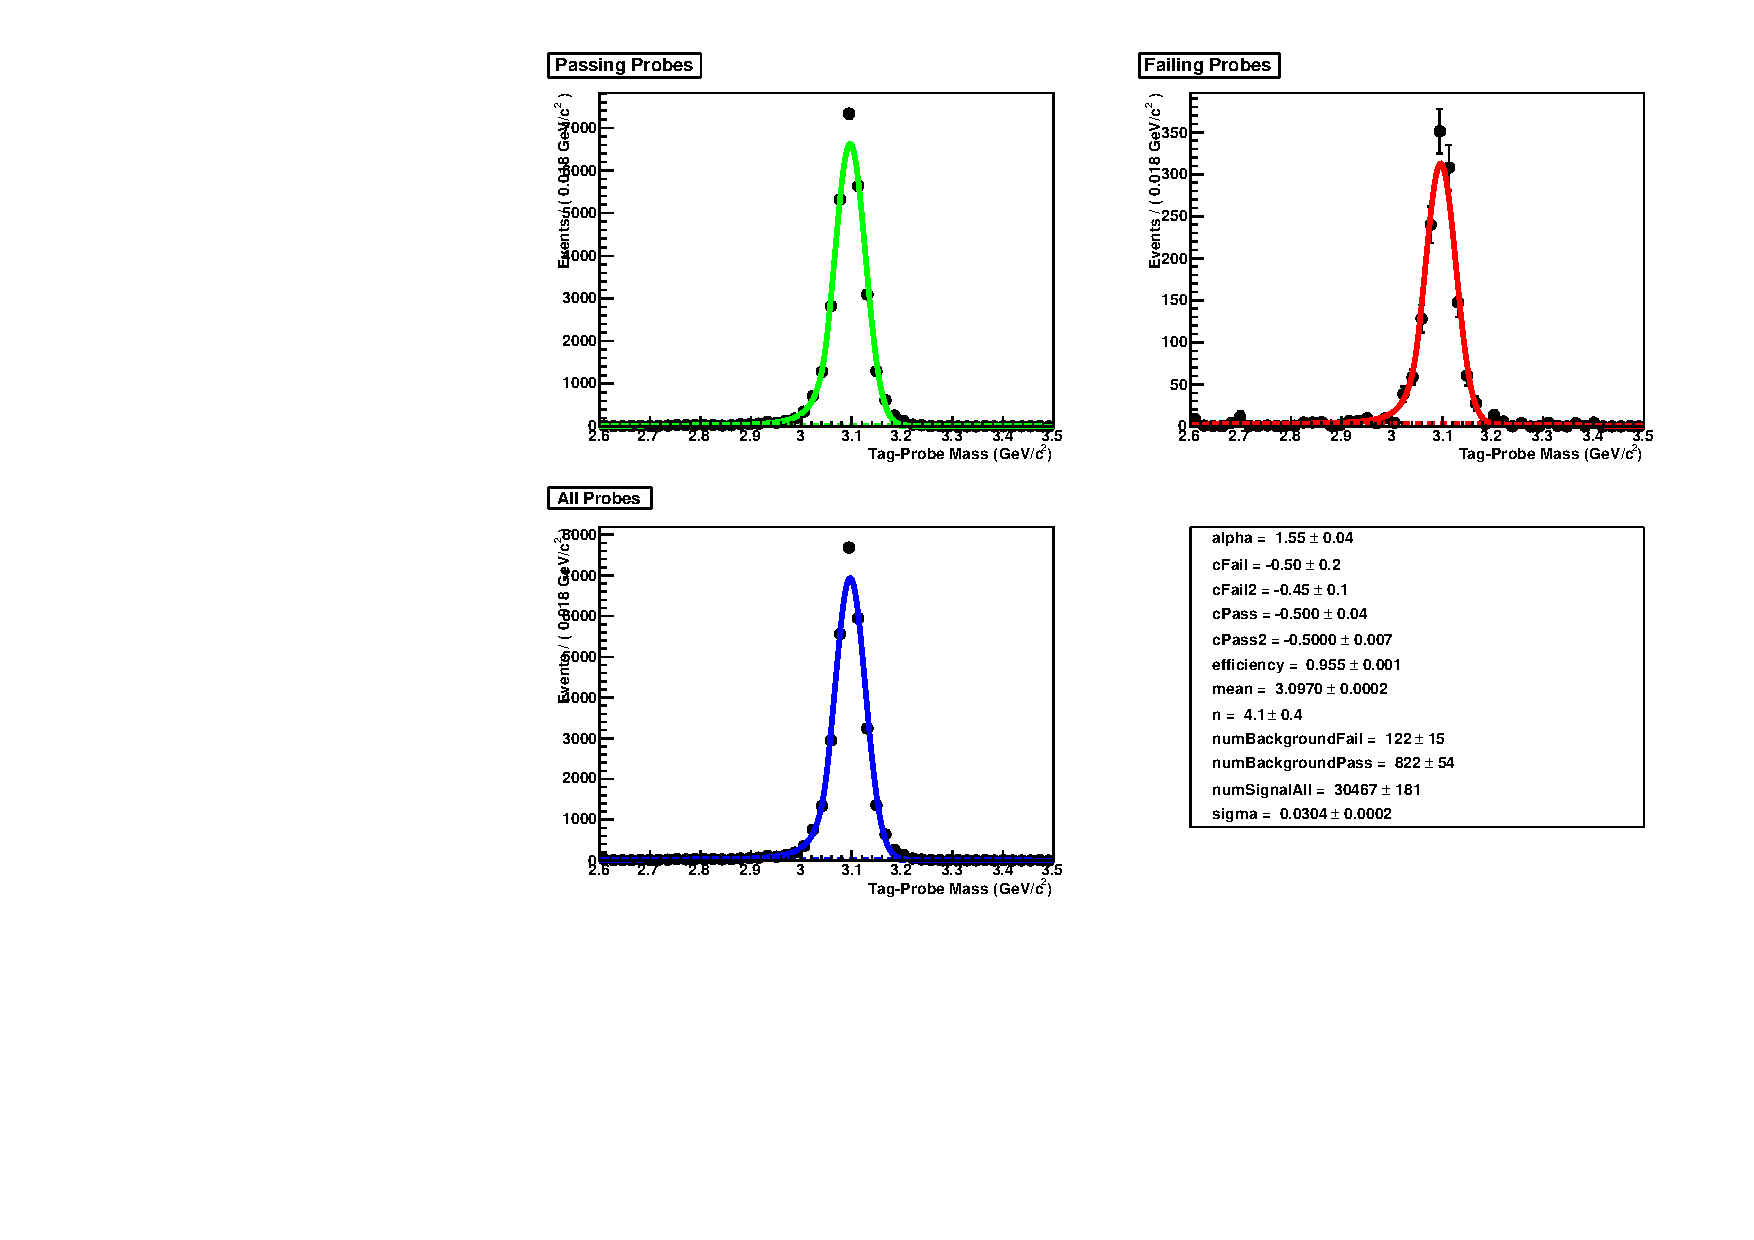
\includegraphics[width=0.9\textwidth]{figures/efficiency/MC_MuId_massfit_0100}}\hspace{1em}
    \subfigure[Simulation]{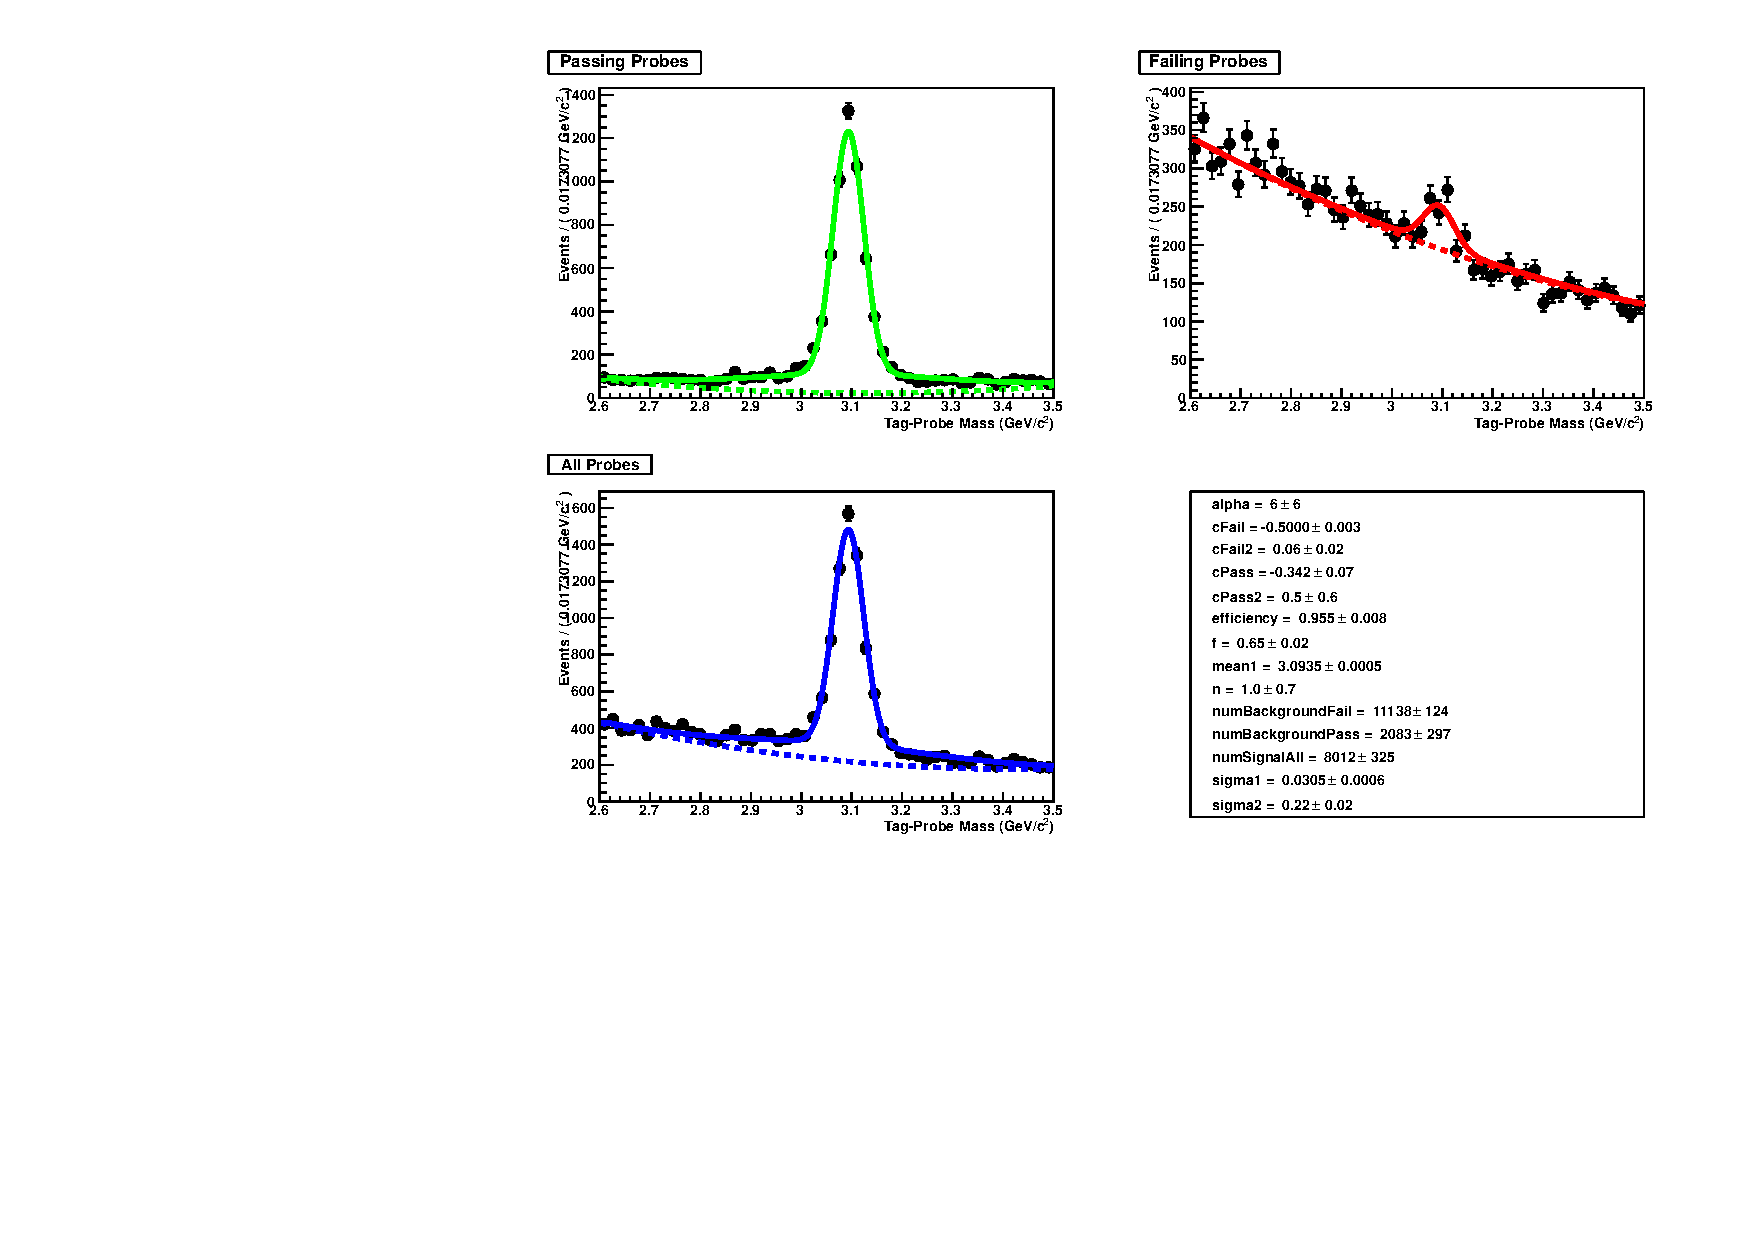
\includegraphics[width=0.9\textwidth]{figures/efficiency/RD_MuId_massfit_0100}}
    \caption{Examples of tag-probe pair mass fits for the muon identification efficiency in MC and data.}
    \label{fig:tnpMuIDFit}
  \end{center}
\end{figure}

\begin{figure}[hp]
  \begin{center}
    \subfigure[Muon id efficiency dependence on muon $\pt$.]{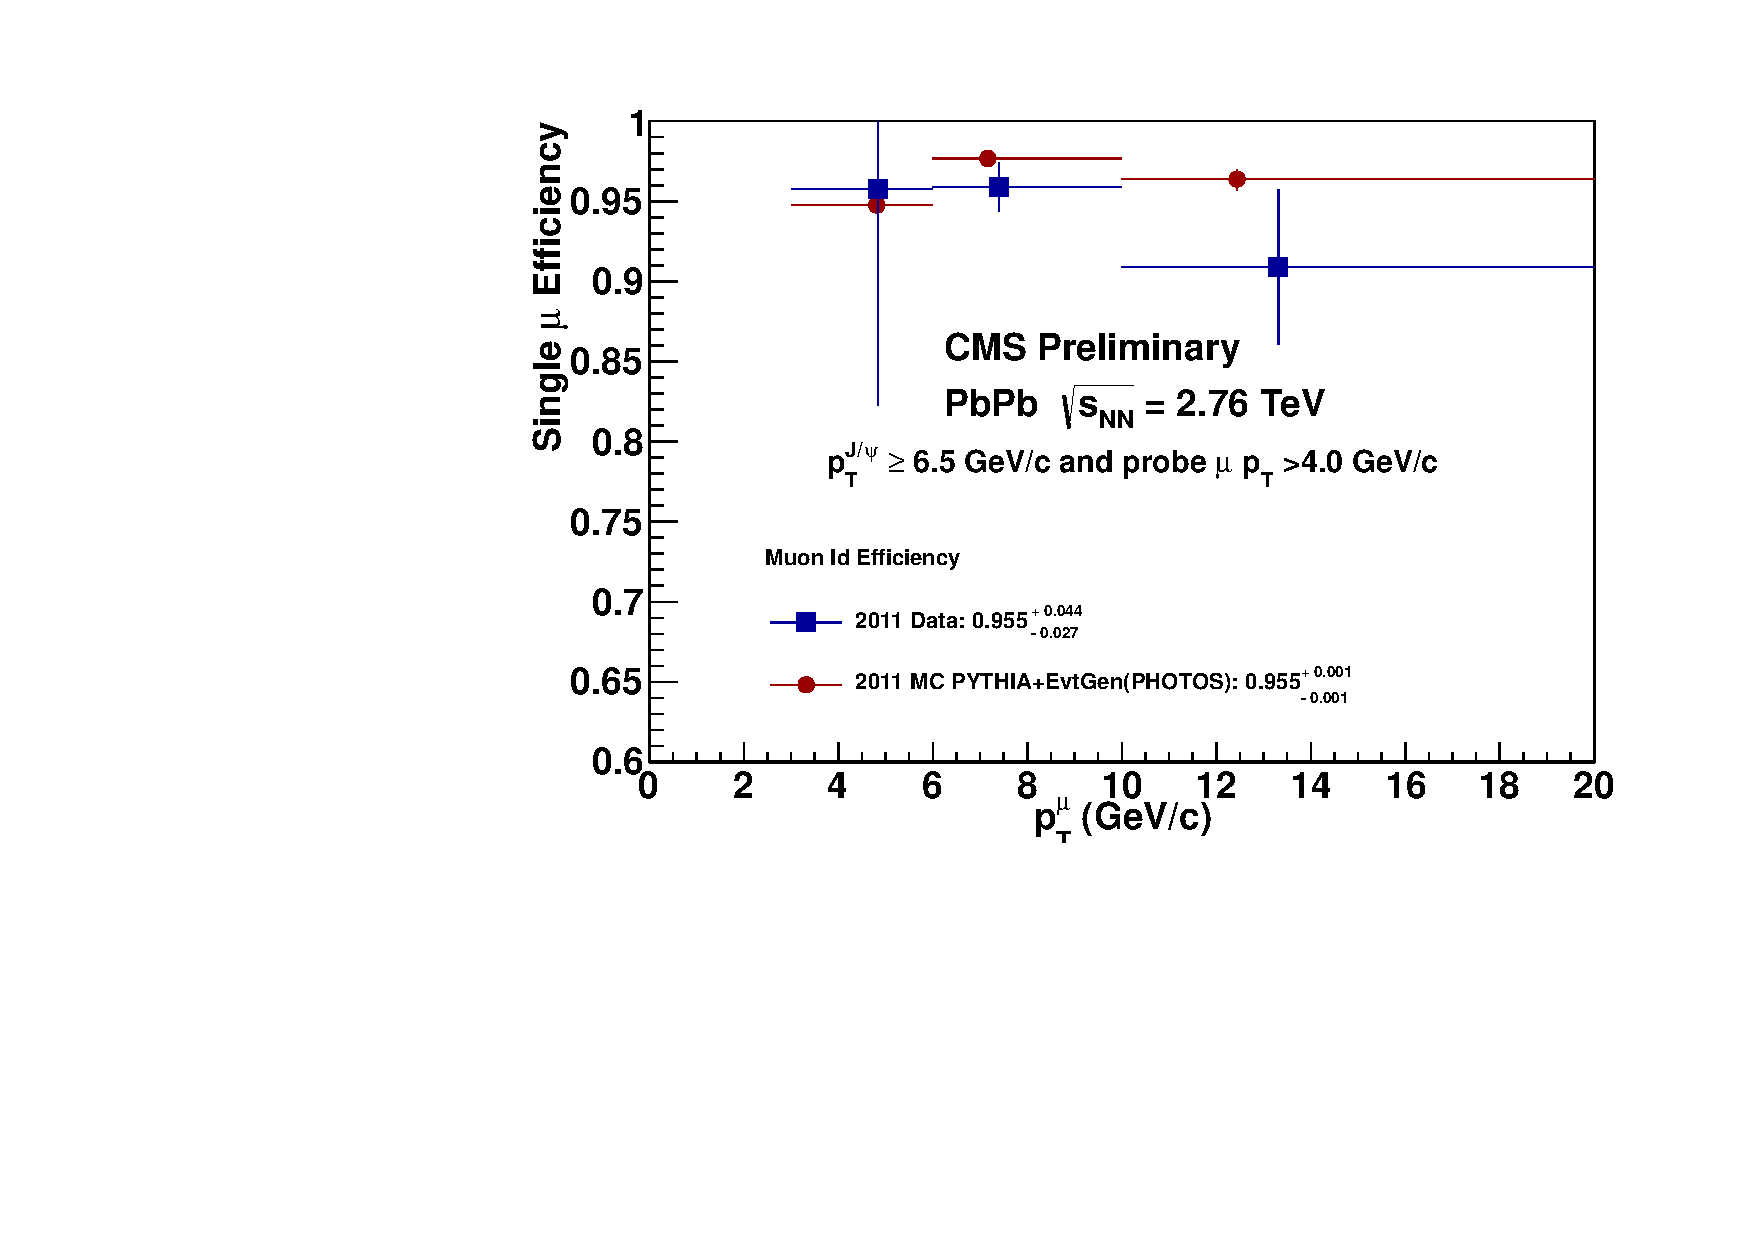
\includegraphics[width=0.6\textwidth]{figures/efficiency/MuID_Comp_pt}} \\ %\hspace{1em}
    \subfigure[Muon id efficiency dependence on muon $\eta$.]{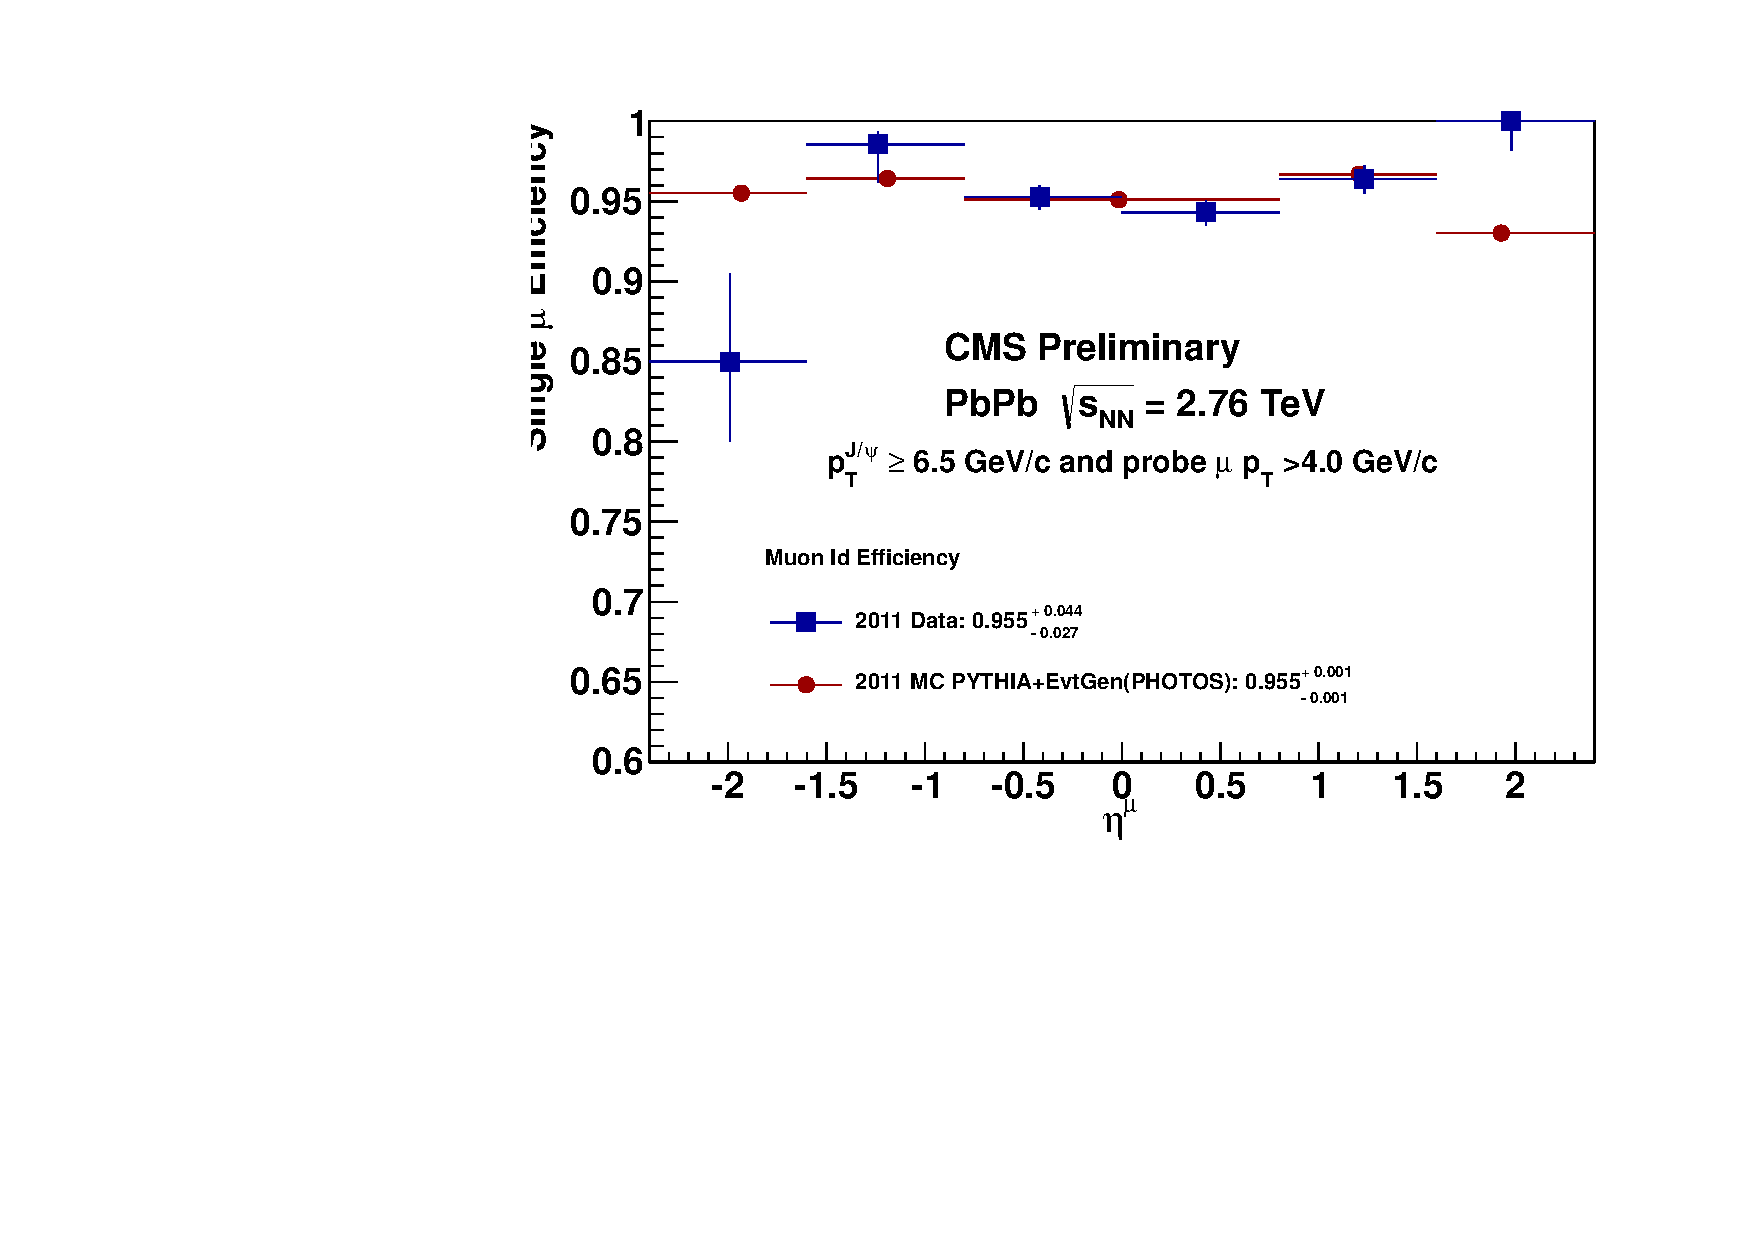
\includegraphics[width=0.6\textwidth]{figures/efficiency/MuID_Comp_eta}} \\
    \subfigure[Muon id efficiency dependence on event centrality.]{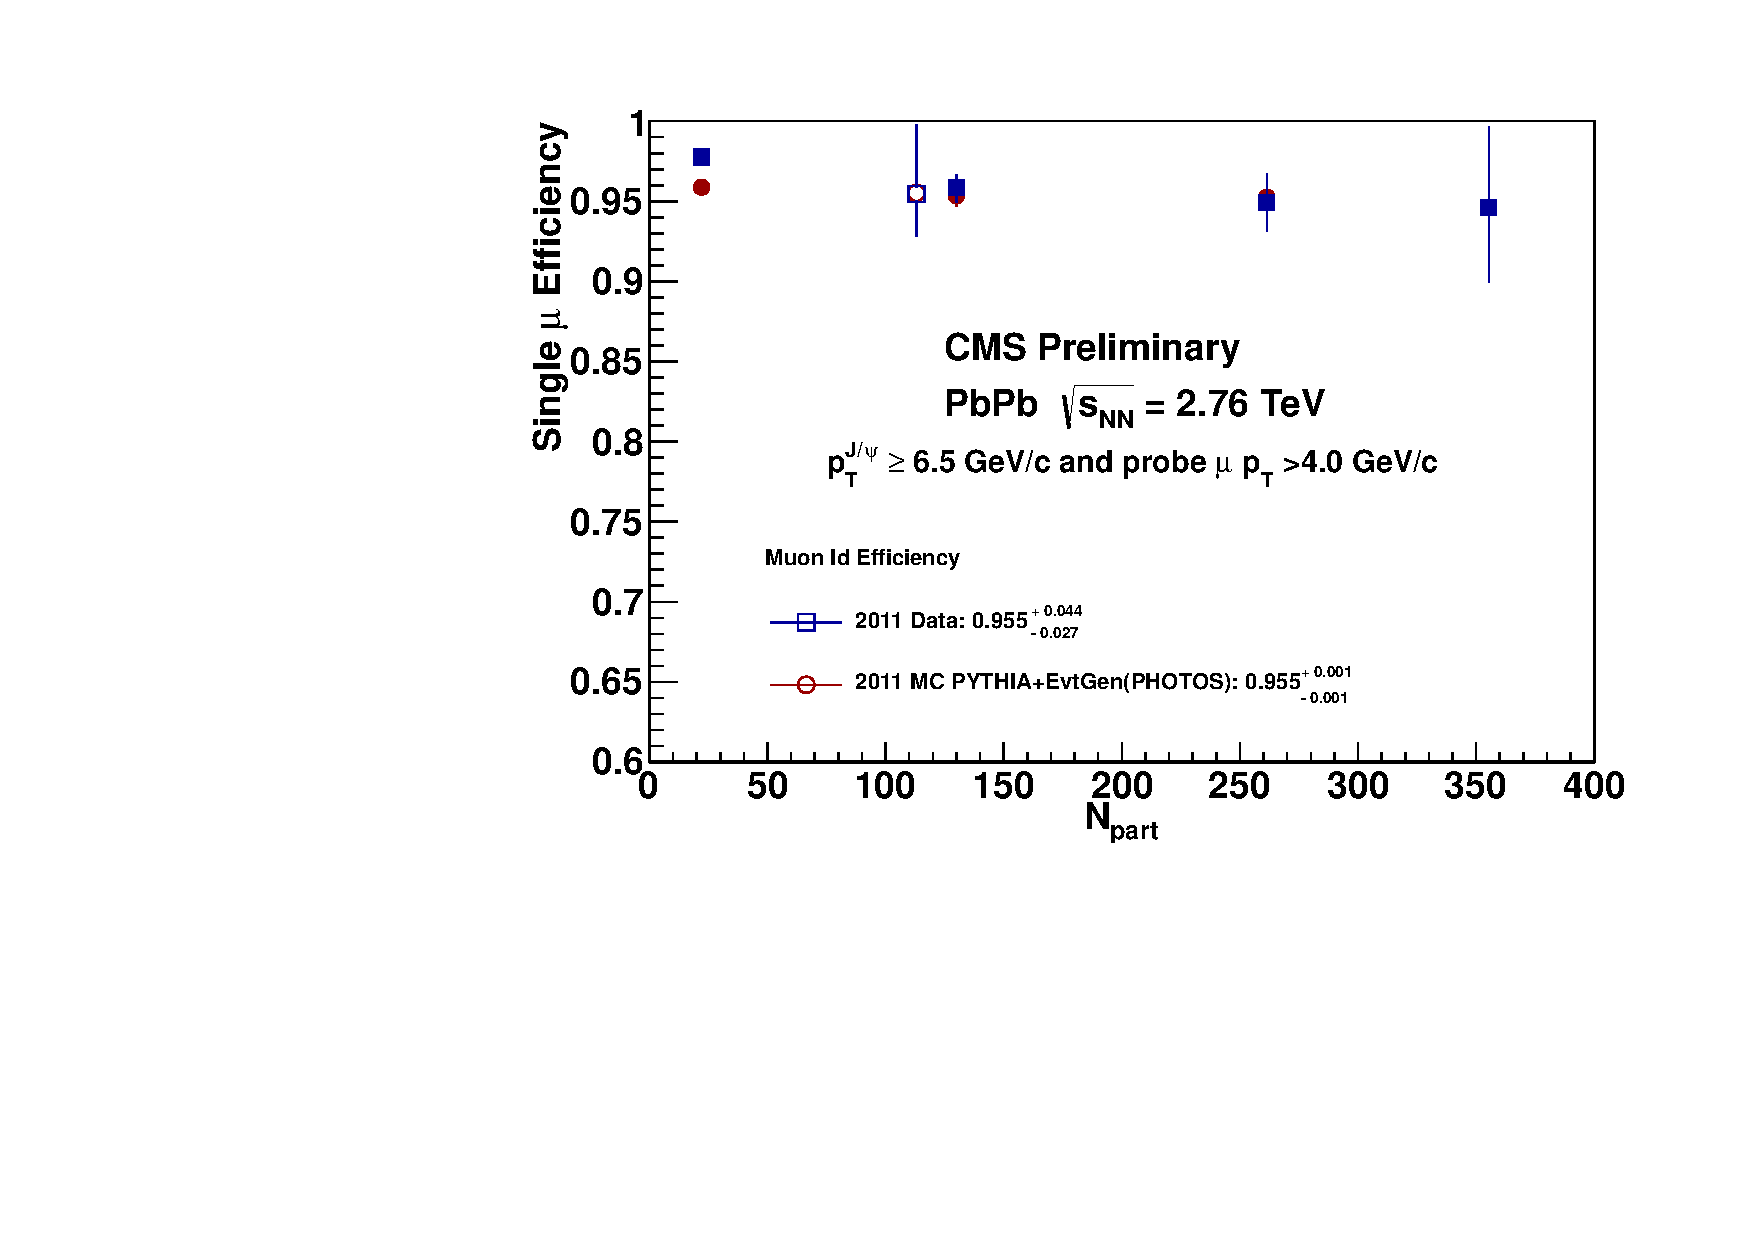
\includegraphics[width=0.6\textwidth]{figures/efficiency/MuID_Comp_cent}}
    \caption{Muon identification efficiency measurements with tag and probe, and dependencies on probe muon \pt and pseudo-rapidity and event centrality. The efficiencies measured in the full samples are represented as open symbols and the corresponding numerical values are displayed for data and simulation.}
%Comparison of the trigger efficiency measured with Tag and Probe in 2011 \emph{(blue squares and pink stars)} and 2010  \emph{(red circles and green triangles)} data, as function of \pt \emph{(left)}, $\eta$ \emph{(right)} and centrality \emph{(bottom)}.}
    \label{fig:tnpMuIDEff} %TBD: update these
  \end{center}
\end{figure}


\subsubsection{Tracking efficiency}

%Given the poorer mass resolution (based on stadalone muon \pt probe measurements), an enlarged fitting range is used. 
%In addition to the \Jpsi, also the contribution from the $\Psi^\prime$ needs to be accounted for in the mass fits.

The fits for the tracking efficiency are challenging due to the poor resolution of the standalone muons used as probes. For the same reason, an enlarged fitting range is used. 
A Crystal Ball (and an additional Gaussian when needed to account for different event resolutions, eg for the MC fits) is chosen to describe the signal shape with all its parameters left to float. The background is described by a third order polynomial. 
%Notice that the invariant mass region used was considerably greater. For the MC case we used a Crystal Ball plus a Gaussian in order to account for varying detector resolution effects. 
%However, it must be noticed that the final efficiencies presented here were not extracted from the fitting results but from a counting method which is, together with fitting and side band subtraction, another option in the T\&P package. 

T\&P mass fits for the tracking case are shown in \fig{fig:tnpTrkFit}, for the integrated data and MC samples.
These illustrate the considerably large level of background involved, and the degraded mass resolution. 
%No dimuon-muon \pt selection is applied as the stadalone muon measurement is not sufficiently precise.  
%
Shown in \fig{fig:tnpTrkEff} is the tracking efficiency as function of the probe muon \pt and rapidity and event centrality. % for all \Jpsi. 
The MC is seen to overestimate the data, by about 5\%.
%MC and data  show a very good agreement, respectively with 85.0\% and 83.7$^{0.57}_{0.53}$\% for single muon efficiency. 
%Twice this difference, 4.6\%, is used as a  systematics on the corrected dimon yields. 
%No significant centrality dependence is observed in MC, while in data, there seem to be a drop of the efficiency going to the peripheral collisions. 
%This goes in the opposite direction than expectations that efficiency would get lower in a very dense environment but is probably just illustrating fake efficiency in the central bins.
%
%We note this particular measurement is challenging, as anticipated. The measured efficiency values appear to be relatively higher than expected. The systematic is 10.5\%.
%We have tried to switch to tracker muons as probes but it didn't help much as the background is fluctuating a lot with STA resolution. %??? tracker muon contain tracker info, so these are not unbiased probles, right?
%In conclusion,  T\&P tracking results are still being studied. 
%Further studies are still being pursued, including of stricter tag/probe selection, to attempt to better understand the background shape. 
%Some cuts on the tags \pt might help understand the background shape better.

\begin{figure}[hp]
  \begin{center}
    \subfigure[Data]
    {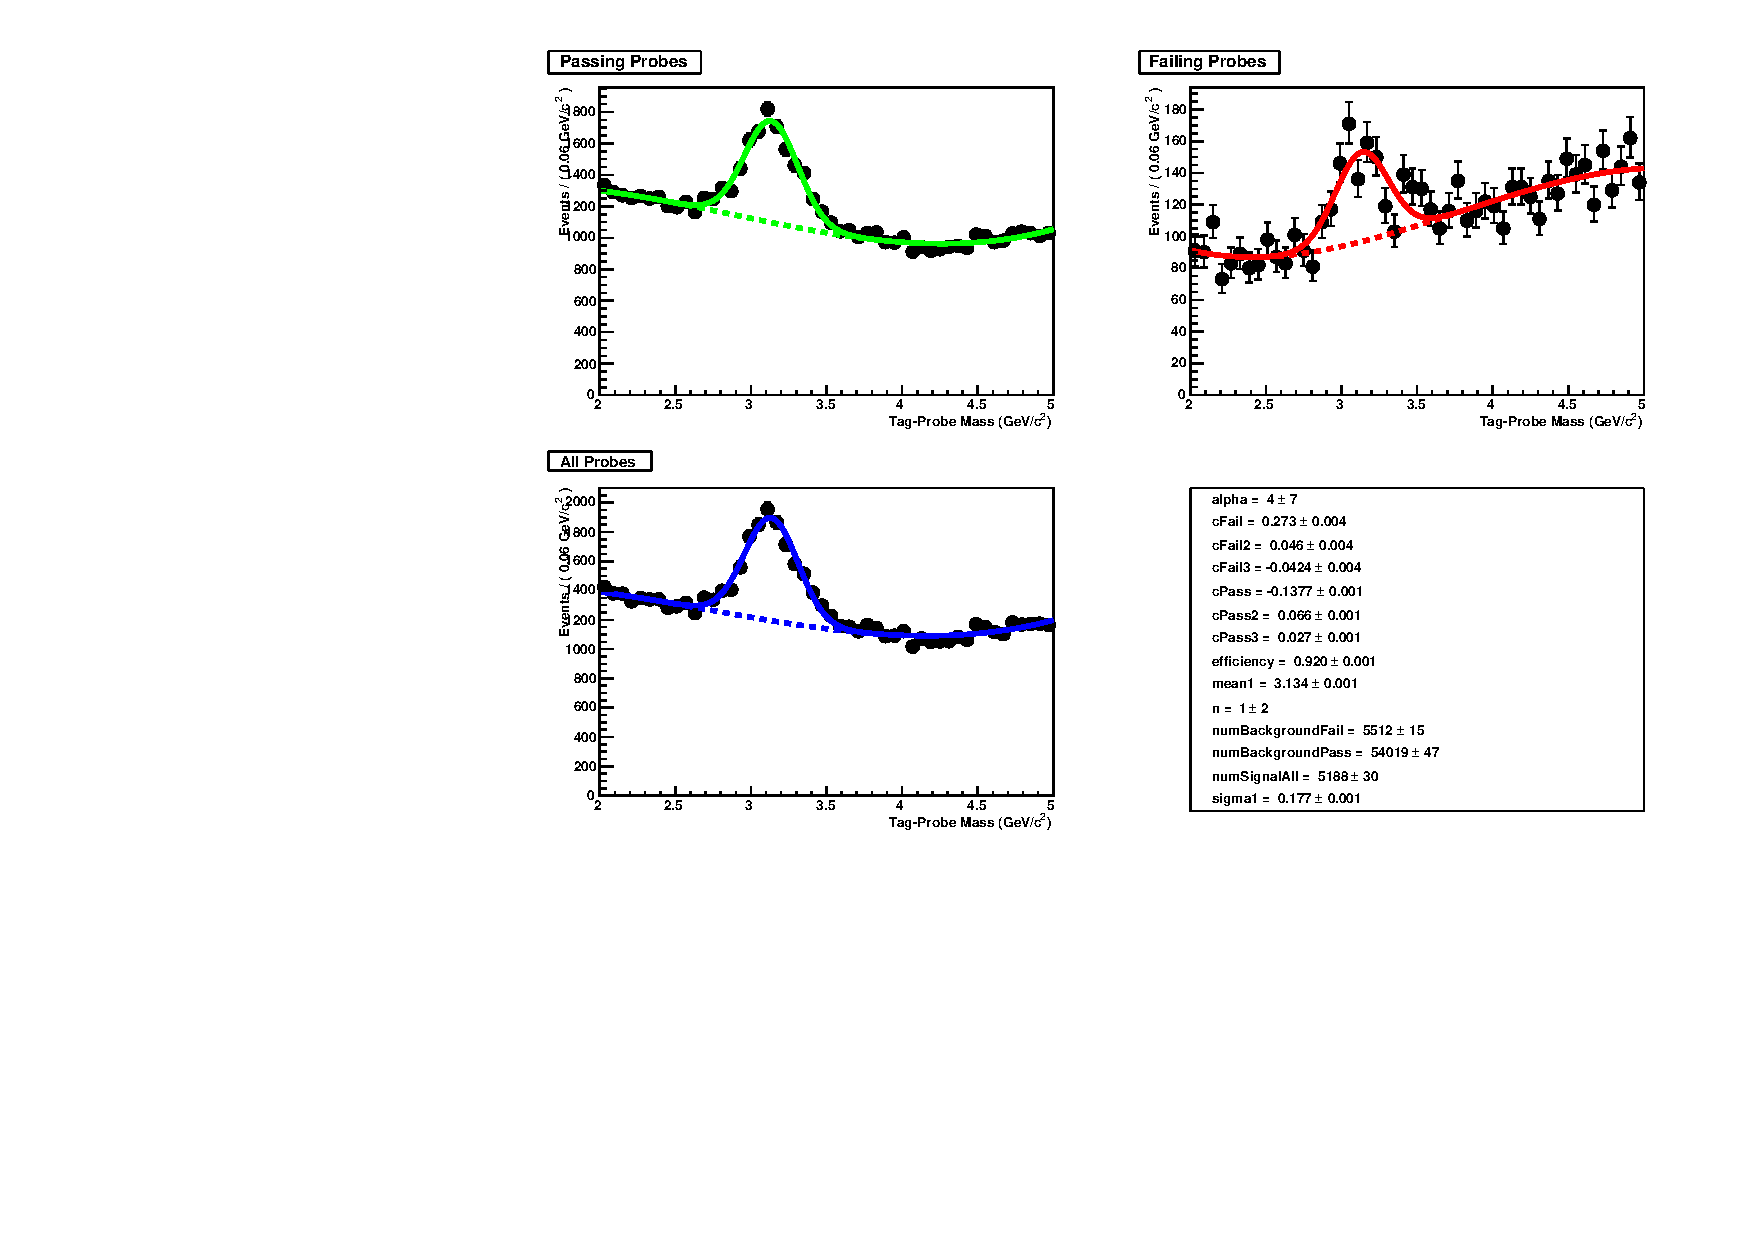
\includegraphics[width=0.9\textwidth]{figures/efficiency/RD_Trk_massfit_0100}}\hspace{1em}
    \subfigure[Simulation]
    {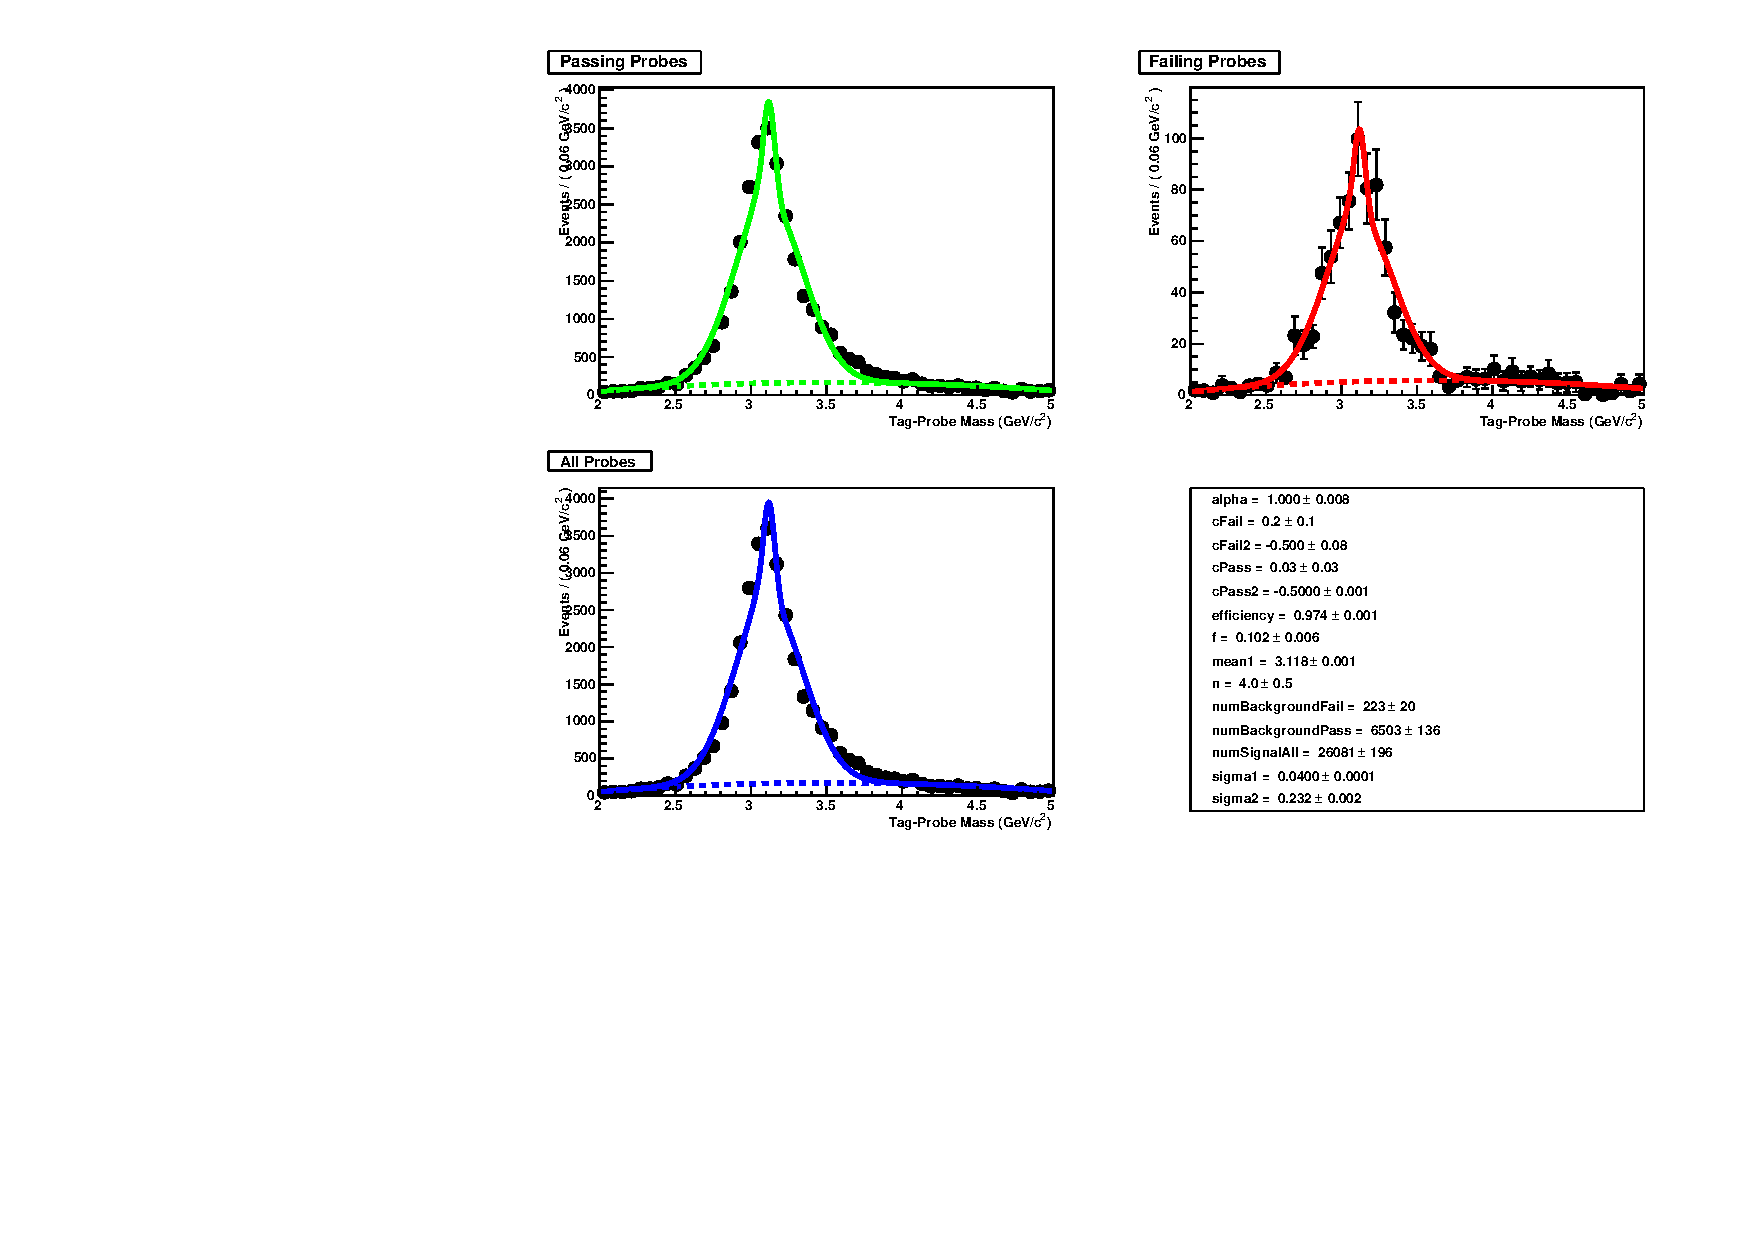
\includegraphics[width=0.9\textwidth]{figures/efficiency/MC_Trk_massfit_0100}}
    \caption{Examples of tag-probe pair mass fits for the inner tracking efficiency.}
    \label{fig:tnpTrkFit}
  \end{center}
\end{figure}

\begin{figure}[hp]
  \begin{center}
    \subfigure[Tracking efficiency dependence on muon $\pt$.]{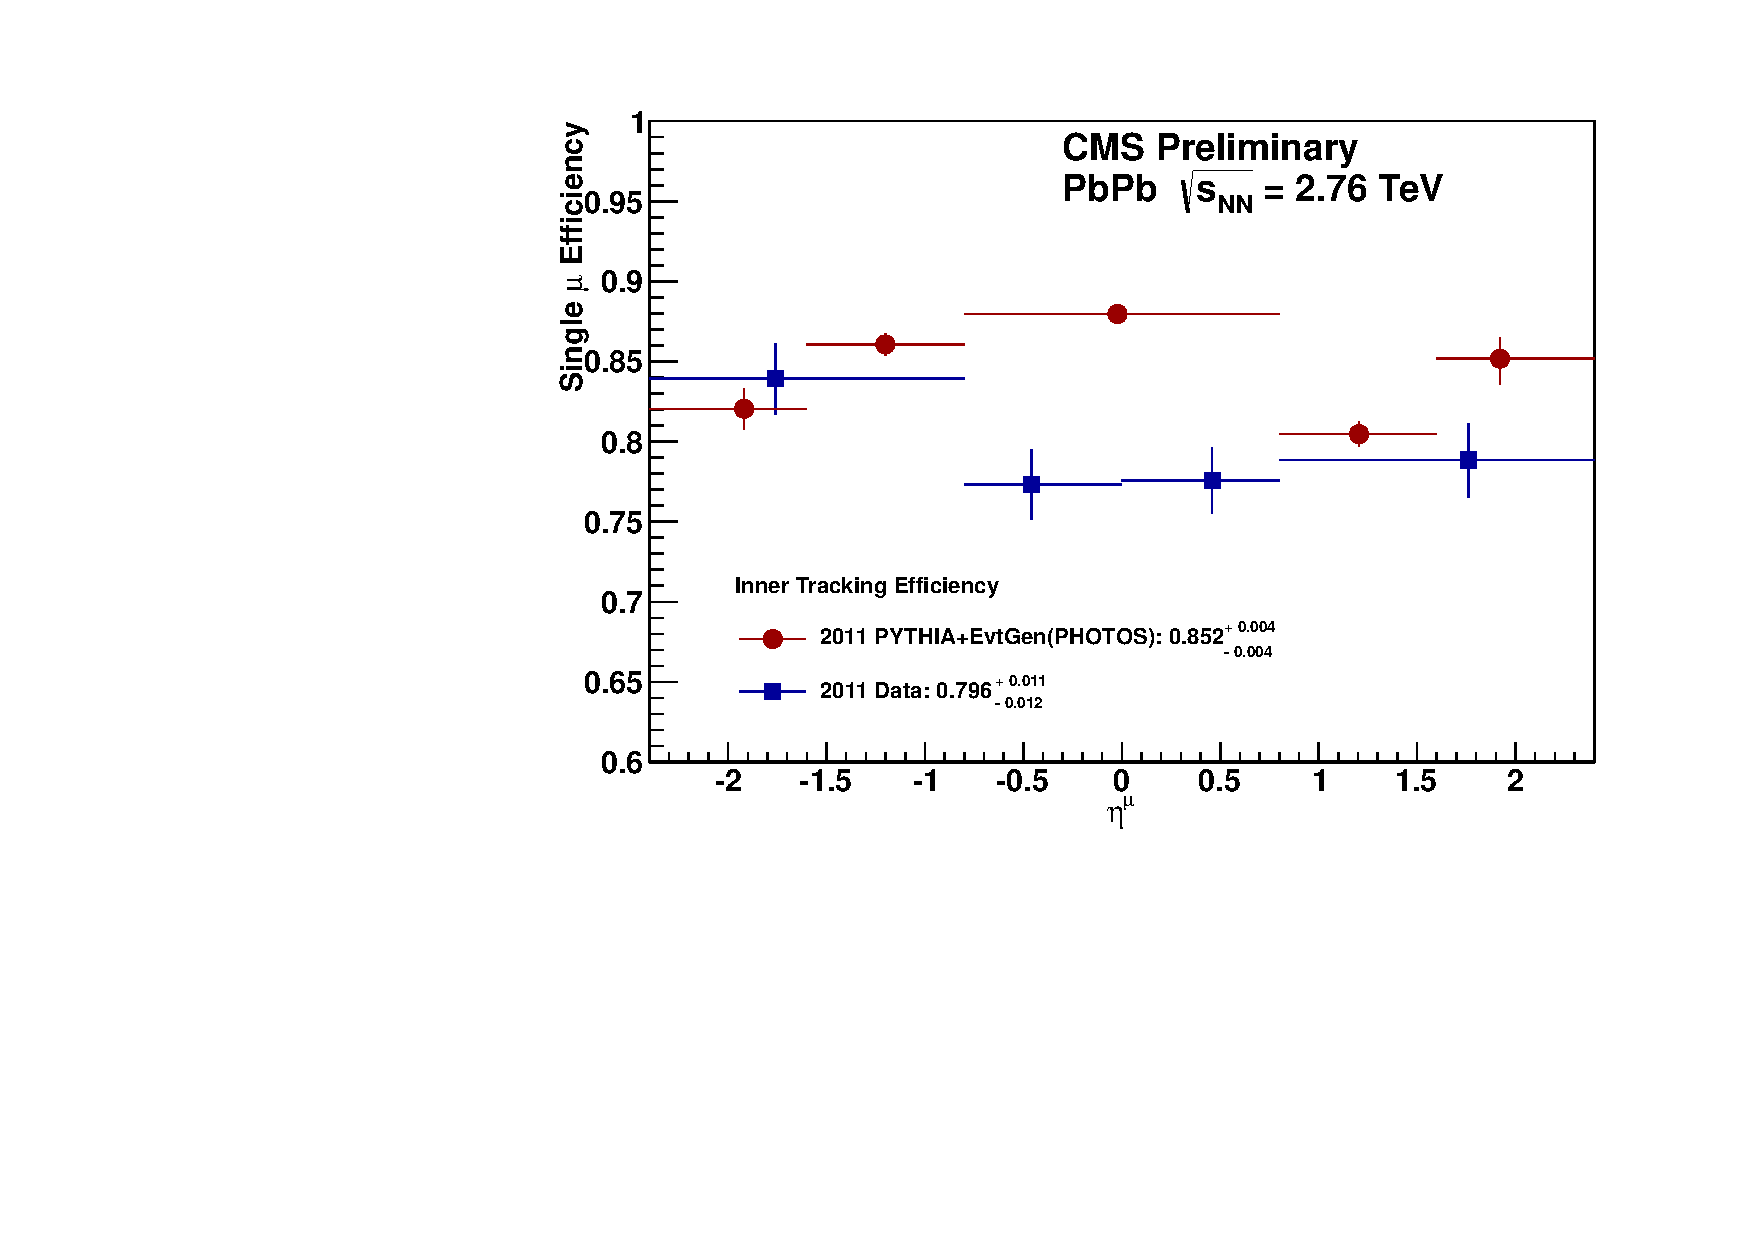
\includegraphics[width=0.6\textwidth]{figures/efficiency/Trk_Comp_eta_MC_RD_highPt_notriggermatched}}  \\ %\hspace{1em}
    \subfigure[Tracking efficiency dependence on muon $\eta$.]{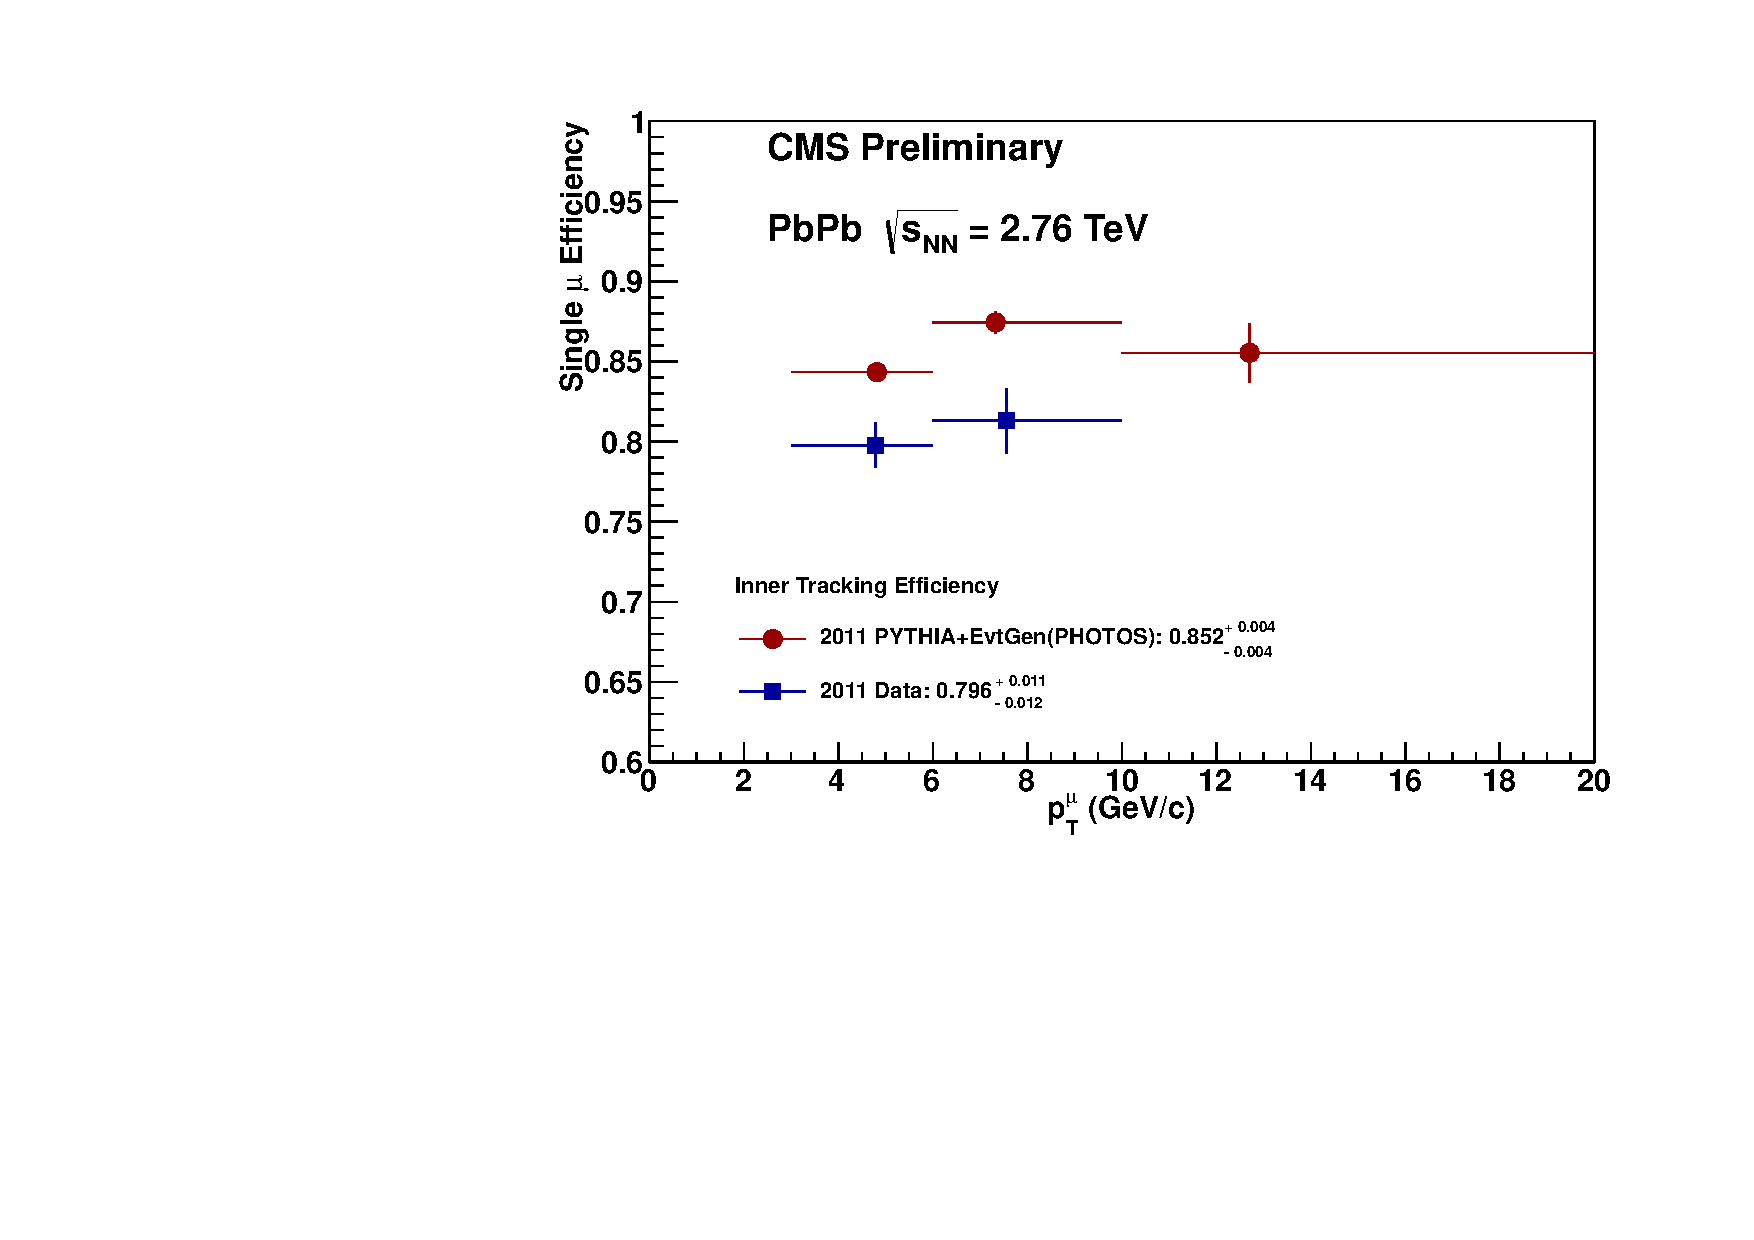
\includegraphics[width=0.6\textwidth]{figures/efficiency/Trk_Comp_pt_MC_RD_HighPt_notriggermatched.pdf}} \\
    \subfigure[Tracking efficiency dependence on event centrality.]{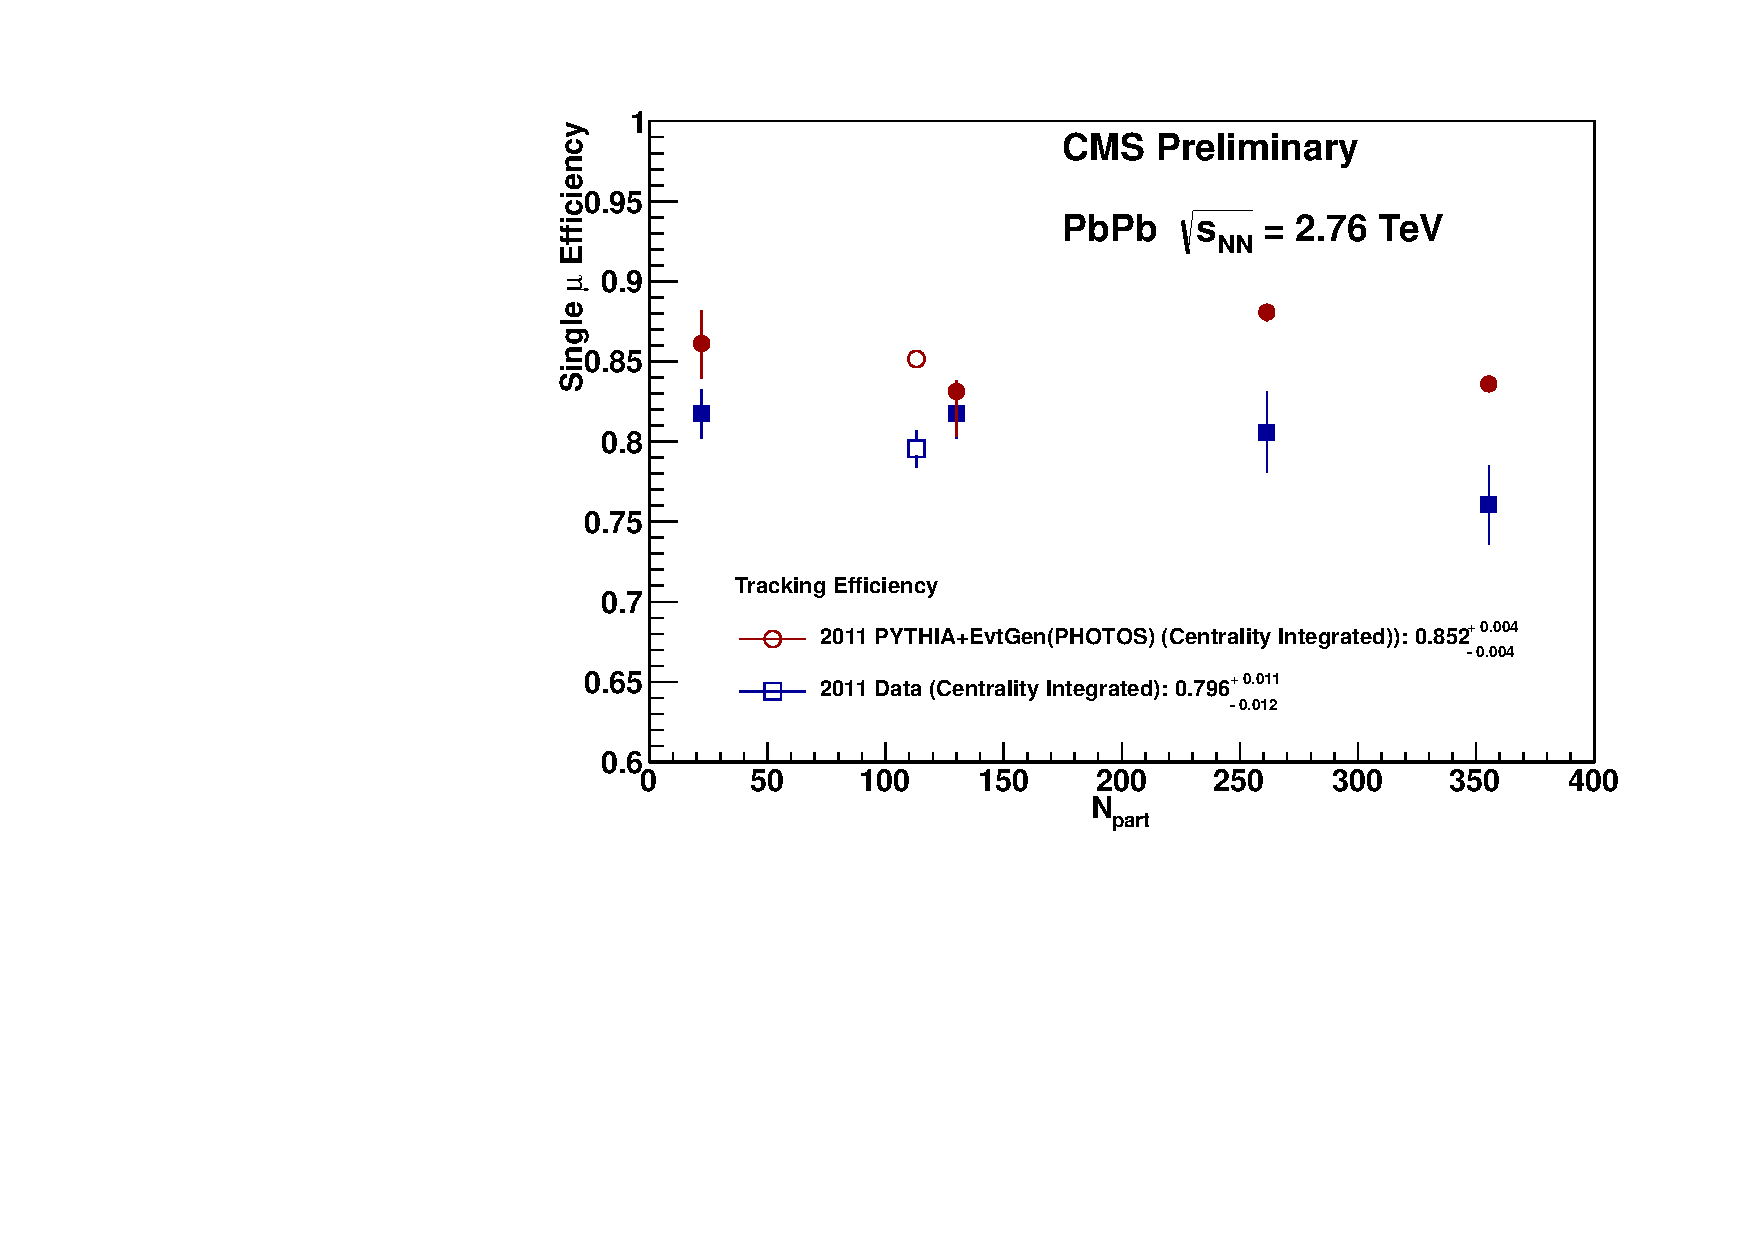
\includegraphics[width=0.6\textwidth]{figures/efficiency/Trk_Comp_CNT_MC_RD_highPt_notriggermatched}}
    \caption{Tracking efficiency measurements with tag and probe, and dependencies on probe muon \pt and pseudo-rapidity and event centrality. The efficiencies measured in the full samples are represented as open symbols and the corresponding numerical values are displayed for data and simulation.}
    \label{fig:tnpTrkEff} %TBD: update!
  \end{center}
\end{figure}

Finally we summarize in Table~\ref{tab:TnPEffTable} all the efficiency estimations as a function of centrality, based on the full data and simulation \PbPb samples.
%
\begin{table}[h!]
\begin{center}
\caption{Tag and probe efficiency measurements in \PbPb data and simulation; 
an acceptance cut $\pt^{\mu} > 4.0 \GeVc$ on the probe muons is applied; 
values are in percent, and errors are statistical only.} 
%n and reconstruction efficiency for data and MC. .
\label{tab:TnPEffTable}
\begin{tabular}{c|cc|cc|cc}
\hline
          \PbPb & \multicolumn{2}{c}{Muon Identification} & \multicolumn{2}{|c}{Trigger} & \multicolumn{2}{|c}{Tracking} \\
centrality& MC   & data & MC   & data & MC   &data   \\
\hline
0-10\%    & $94.6 \pm 0.2$ & $94.6 \pm 5.0$ & $93.9 \pm 2.1$ & $96.7 \pm 0.5$ & $83.6 \pm 0.4 $ & $76.1 \pm 2.5 $   \\
10-20\%   & $95.3 \pm 0.3$& $94.9 \pm 1.8$& $95.1 \pm 4.8$ & $96.9 \pm 0.5$ & $88.0 \pm 0.6 $ & $80.6 \pm 2.5 $  \\
20-50\%   & $95.3 \pm 0.2$ & $95.8 \pm 2.5$ & $94.4 \pm 0.7$ & $96.7 \pm 0.4$& $ 83.1 \pm 2.0 $ & $81.7 \pm 1.5 $ \\
50-100\%  & $95.9 \pm 0.6$ & $97.8 \pm 0.8$ & $94.3 \pm 0.7$ & $96.8 \pm 3.2$& $86.1 \pm 2.0 $ & $81.7 \pm 1.5 $  \\
0-100\%   & $95.5 \pm 0.1$ & $95.5 \pm 4.4$ & $94.3 \pm 0.1$ & $96.8 \pm 0.2$ & $85.2 \pm 0.3$ & $79.6 \pm 1.2$  \\

%\begin{tabular}{c|c|c}

%  \hline
% & data & MC \\
%  \hline
%  Trigger              &  $ 97.2 \pm  0.3 $ & $ 94.3 \pm 0.1 $ \\
%  Muon Identification  &  $ 95.5 \pm  0.8 $ & $ 95.5 \pm 0.1 $ \\
%  Tracking             &  $ 85.2 \pm  0.3 $ & $ 79.6 \pm 1.2 $ \\
\hline
\end{tabular}
\end{center}
\end{table}


Table~\ref{tab:TnPEffTablepp} also summarizes the tag and probe results obtained from the \pp data and MC datasets. These studies were performed in the analysis documented in Ref.~\cite{CMS_PAS_HIN-10-006}. While different selection criteria were employed therein, which prevents a direct comparison of results for \pp and \PbPb, this may be used for the purpose of data--simulation systematic estimation.


\begin{table}[h!]
\begin{center}
\caption{Tag and probe efficiency measurements in \pp data and simulation; 
an acceptance cut $\pt^{\mu} > 4.0 \GeVc$ on the probe muons is applied; 
values are in percent, and errors are statistical only; results from~\cite{CMS_PAS_HIN-10-006}.} 
\label{tab:TnPEffTablepp}
\begin{tabular}{c|cc|cc}
\hline
& \multicolumn{2}{|c}{Trigger} & \multicolumn{2}{|c}{Tracking} \\
& MC   & data & MC   &data   \\
\hline
\pp &
​0.943 $\pm$ 0.002 & 0.925 $\pm$ 0.006 &
​0.846 $\pm$ 0.010 &​0.82  $\pm$ 0.02 \\
\hline
\end{tabular}
\end{center}
\end{table}

\end{chapter}


%TBD: remove results from inline text and into tables
\chapter{Upper limits}

The $\PgUc$ peak is not significantly observed in the  mass spectrum in the \PbPb data.
The significance of $\PgUc$ peak is 0.86$\,\sigma$, evaluated form the profile likelihood ratio, as shown in \fig{fig:3S-significance}. In this section we quantify the relative suppression of the 3S signal state.

\begin{figure}[hbtp]
  \begin{center}
{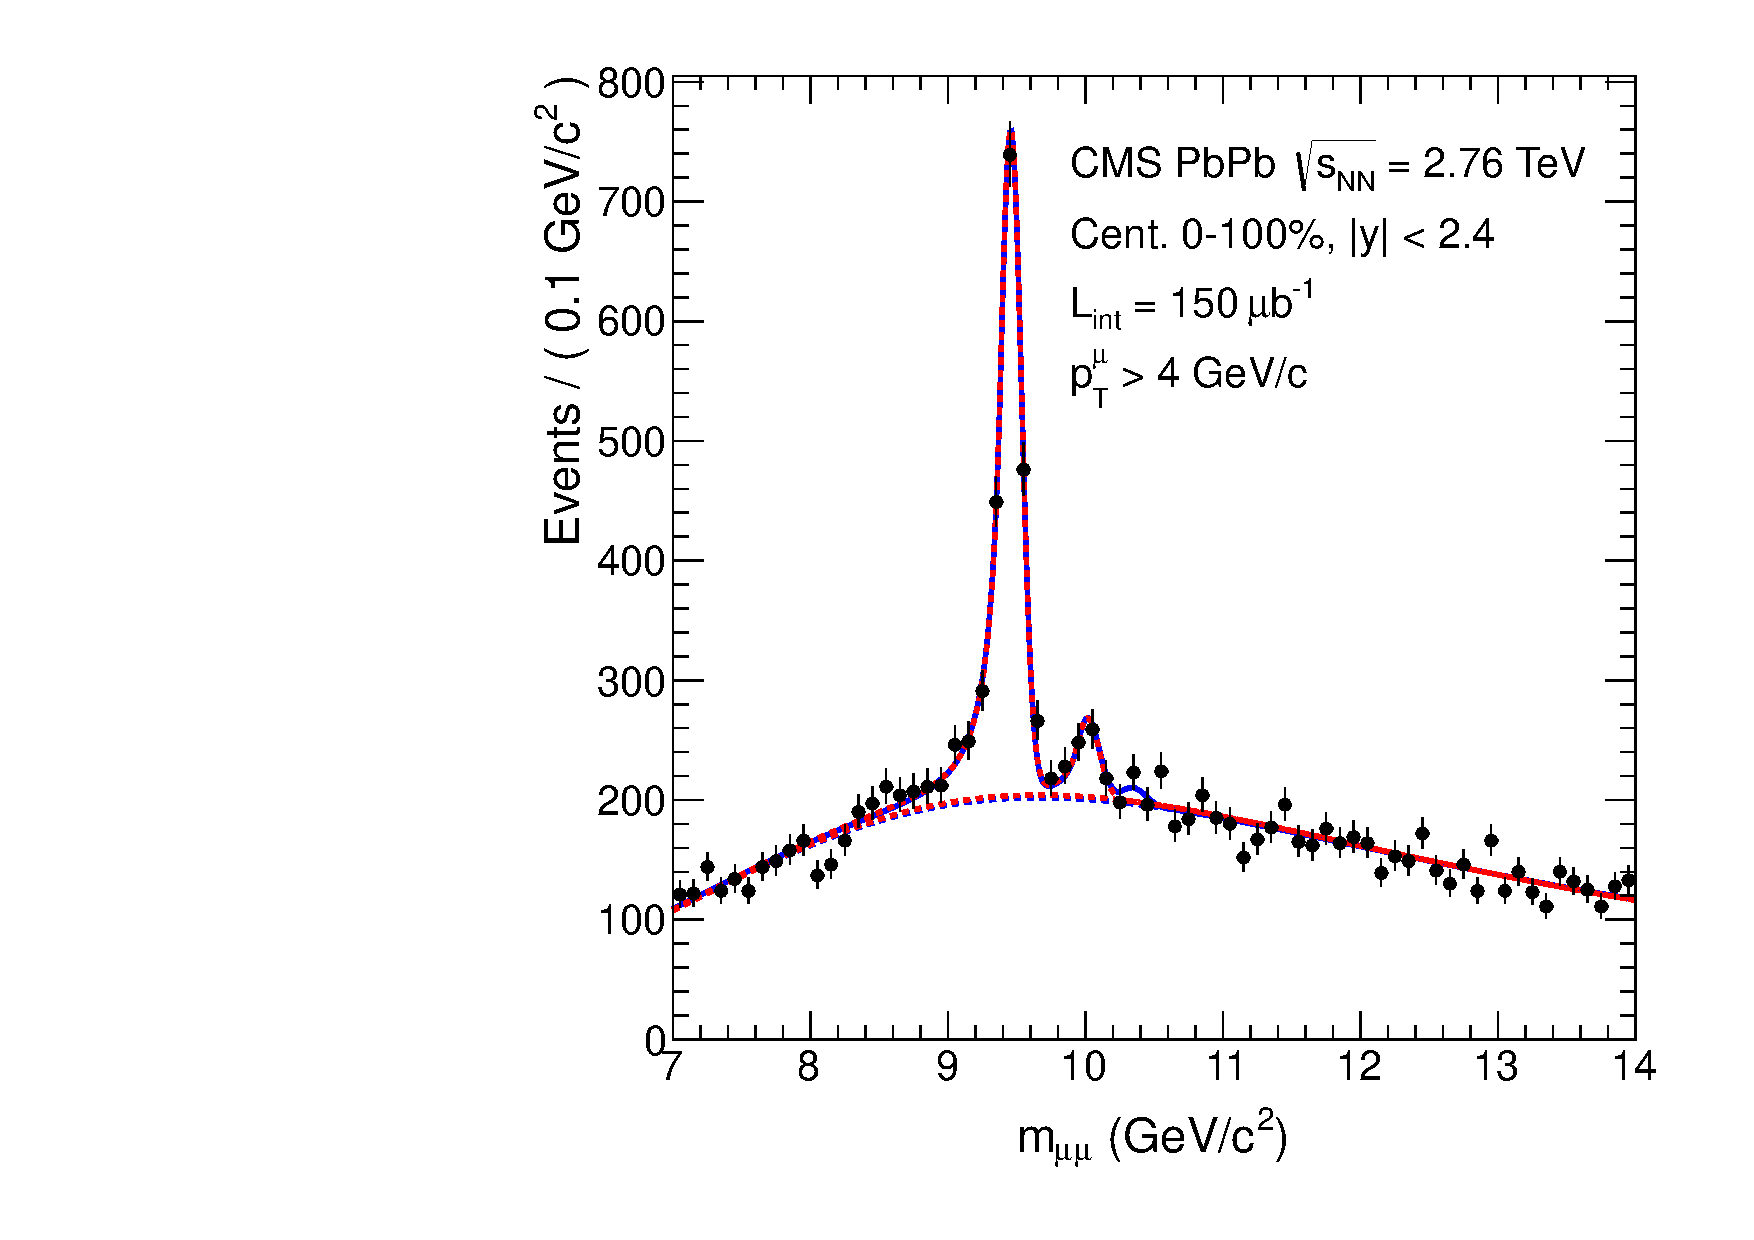
\includegraphics[angle=0,width=0.45\textwidth]{figures/limits/Y3S_significance.pdf}}
   \caption{$\PgUc$ significance, estimated via likelihood ratio, by allowing and disallowing $\PgUc$ p.d.f. in two fits.
}
    \label{fig:3S-significance}
  \end{center}
\end{figure}

%\subsection{The  Feldman-Cousins and $CL_{s}$ prescription}

In some of the centrality bins the data is affected by large downward fluctuations of the background yielding negative yields for the signal \PgUc. We proceed then to set upper limits for the signal 3S .

Approximate methods of confidence interval construction, in particular, the likelihood-ratio method, are often used in order to reduce computation. However, true confidence intervals can be obtained using the original (defining) Neyman construction~\cite{Neyman}.  
Therefore we opted for the unified Feldman-Cousins (FC) approach since this treatment solves the problem whether to set an upper limit or two-sided intervals if the choice is based on the data alone as in our case. 

 As a cross check we also present a pure frequentist approach, the \textit{modified}, or \textit{conservative} $CL_s$ criterion. Here, we use the ratio of $p$-values, $CL_{s}=CL_{sb}/CL_{b}$, instead of the numerator only, to set an upper limit on the single and double ratios involving the 3S.  Finally other implementations based on 95\% credible intervals are presented as cross-checks.

\subsubsection{Single ratio $R_{3}$ limits}
Instead on setting upper limits for the \PgUc signal per se we use the single ratio of the third peak over the first peak ($R_{3}$) in PbPb as our parameter of interest. The idea of the method can be formulated in terms of hypothesis testing in a frequentist approach.  (for an explanation see~\cite{alexread}).  
We define $H_b$ as the alternative hypothesis that no signal 3S is present over the background (single ratio of zero) and $H_{sb}$ the null hypothesis that the signal is indeed present. In order to quantify the degree in which each hypotheses
are favored or excluded by the experimental observation one chooses a
test-statistics which ranks the possible experimental outcomes. A
commonly used test statistics consist as the ratio of the likelihood
function in both hypotheses: $Q=L_{sb}/L_b$, for our study the test statistic of choice is $-2\ln Q$. 

We introduce the systematic uncertainties into the model via a nuisance parameter. Variation of such parameter corresponds to certain systematic uncertainty. The nuisance parameter is either profiled or marginalized depending on whether we are using the frequentist approach or the Bayesian one. 

The computed 95\% CL upper limit with FC is: 0.0737 +/- 0.0014.
%https://espace.cern.ch/cms-heavyion/upsilon/fitting/Upper%20Limits.aspx
Cross checks based on alternative methods are provided in Appendix~\ref{sec:app_limits}. 


\begin{figure}[hbtp]
  \begin{center}
{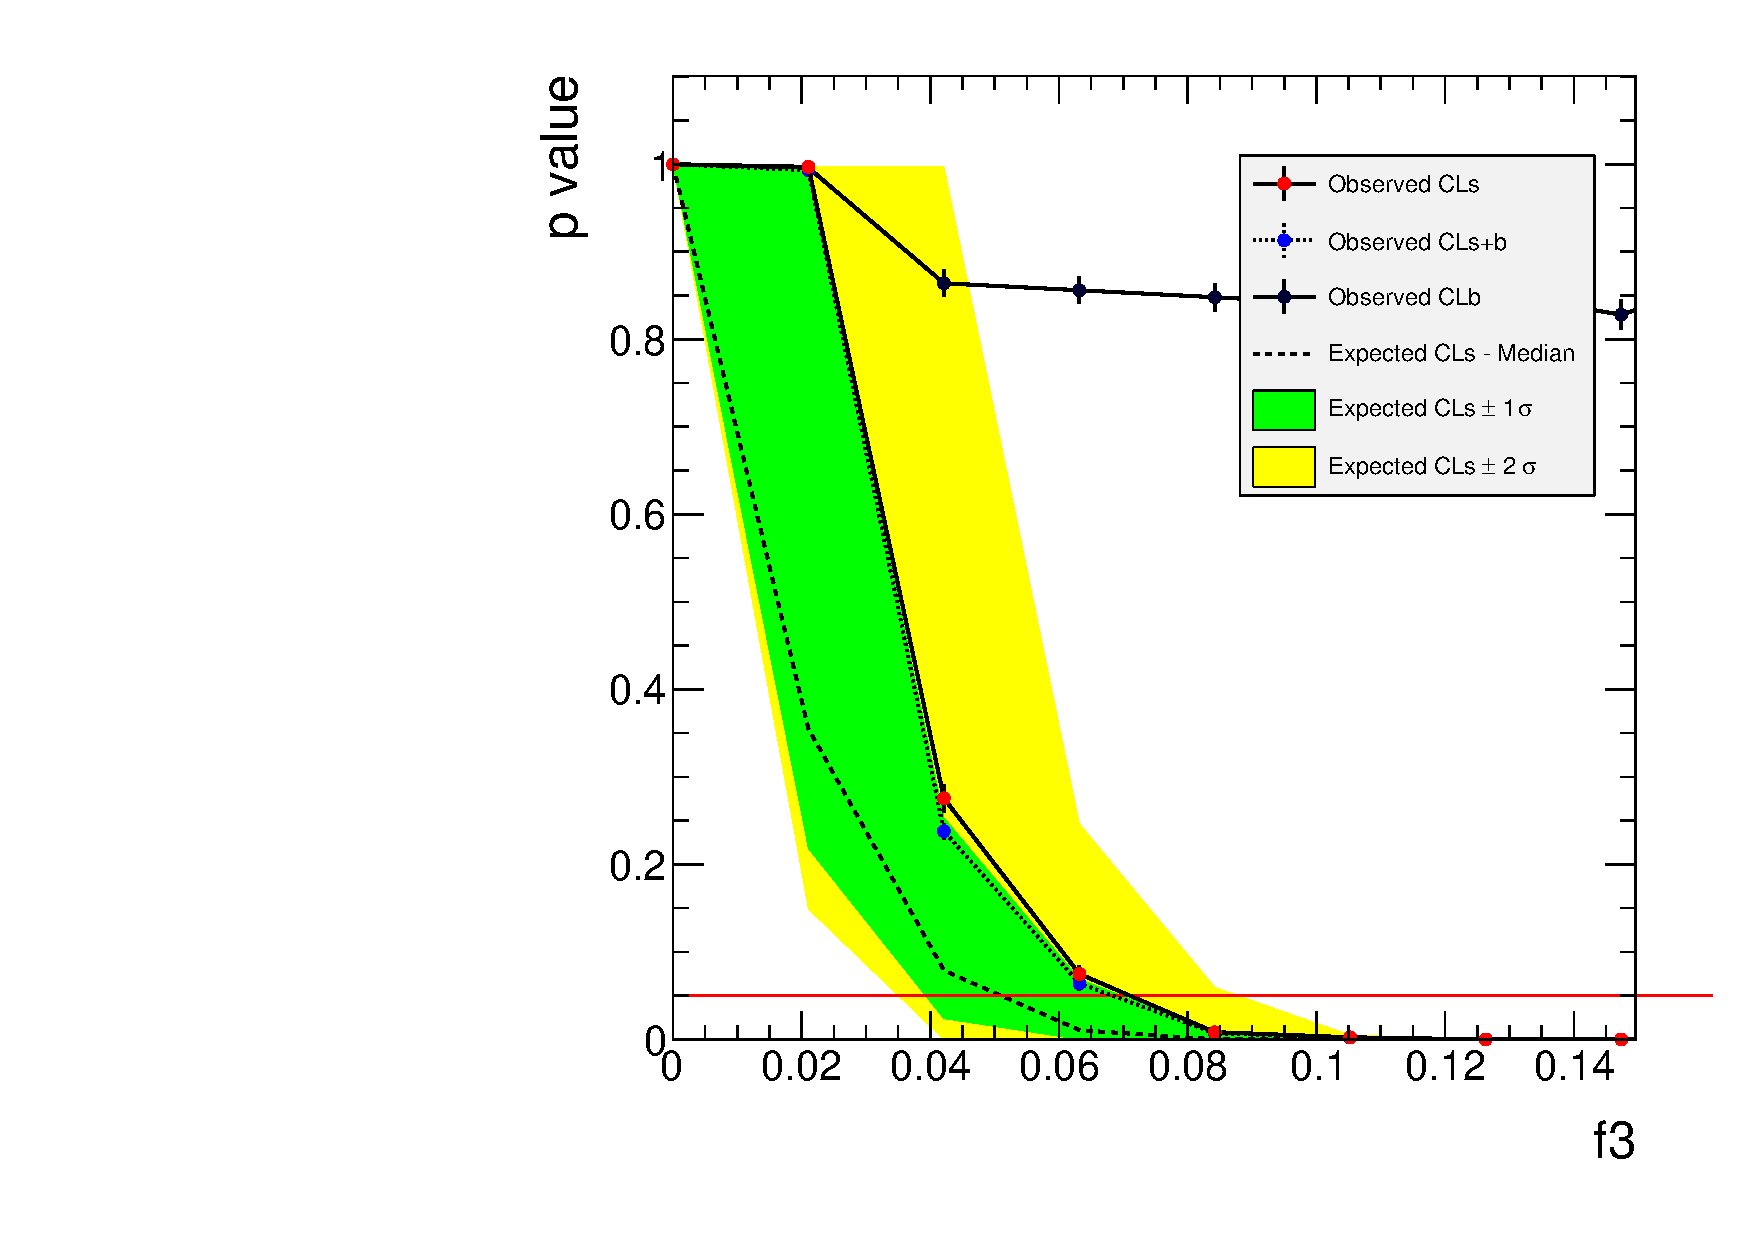
\includegraphics[angle=0,width=0.45\textwidth]{figures/limits/FC_0100}}
   \caption{Upper limit results for $R_3$ in \PbPb using the Feldman-Cousins method.
Shown is a $p$-value scan using 1000 pseudo experiments for each scanned point.  
The 95\% C.L. upper limit corresponds to the point where the observed CLs crosses the 0.05 horizontal/red line. 
%\emph{(Note: being updated)}
%Fig.~\ref{fig:FC_Centrality}: Upper limits vs number of participants using Feldman-Cousins.
}
    \label{fig:FC_results}
  \end{center}
\end{figure}



\subsubsection{Double ratio $\chi_{3}$ limits}

The same statistical instruments shown above are also used to set the limits for double ratio $\chi_{3}$.
Employing the Feldman Cousins technique, the upper limit at 95\% C.L. 
 is $\chi_{3} \leq 0.173 \pm 0.021$,  
as represented in \fig{fig:FCx3_0100}. 

\begin{figure}[hbtp]
  \begin{center}
    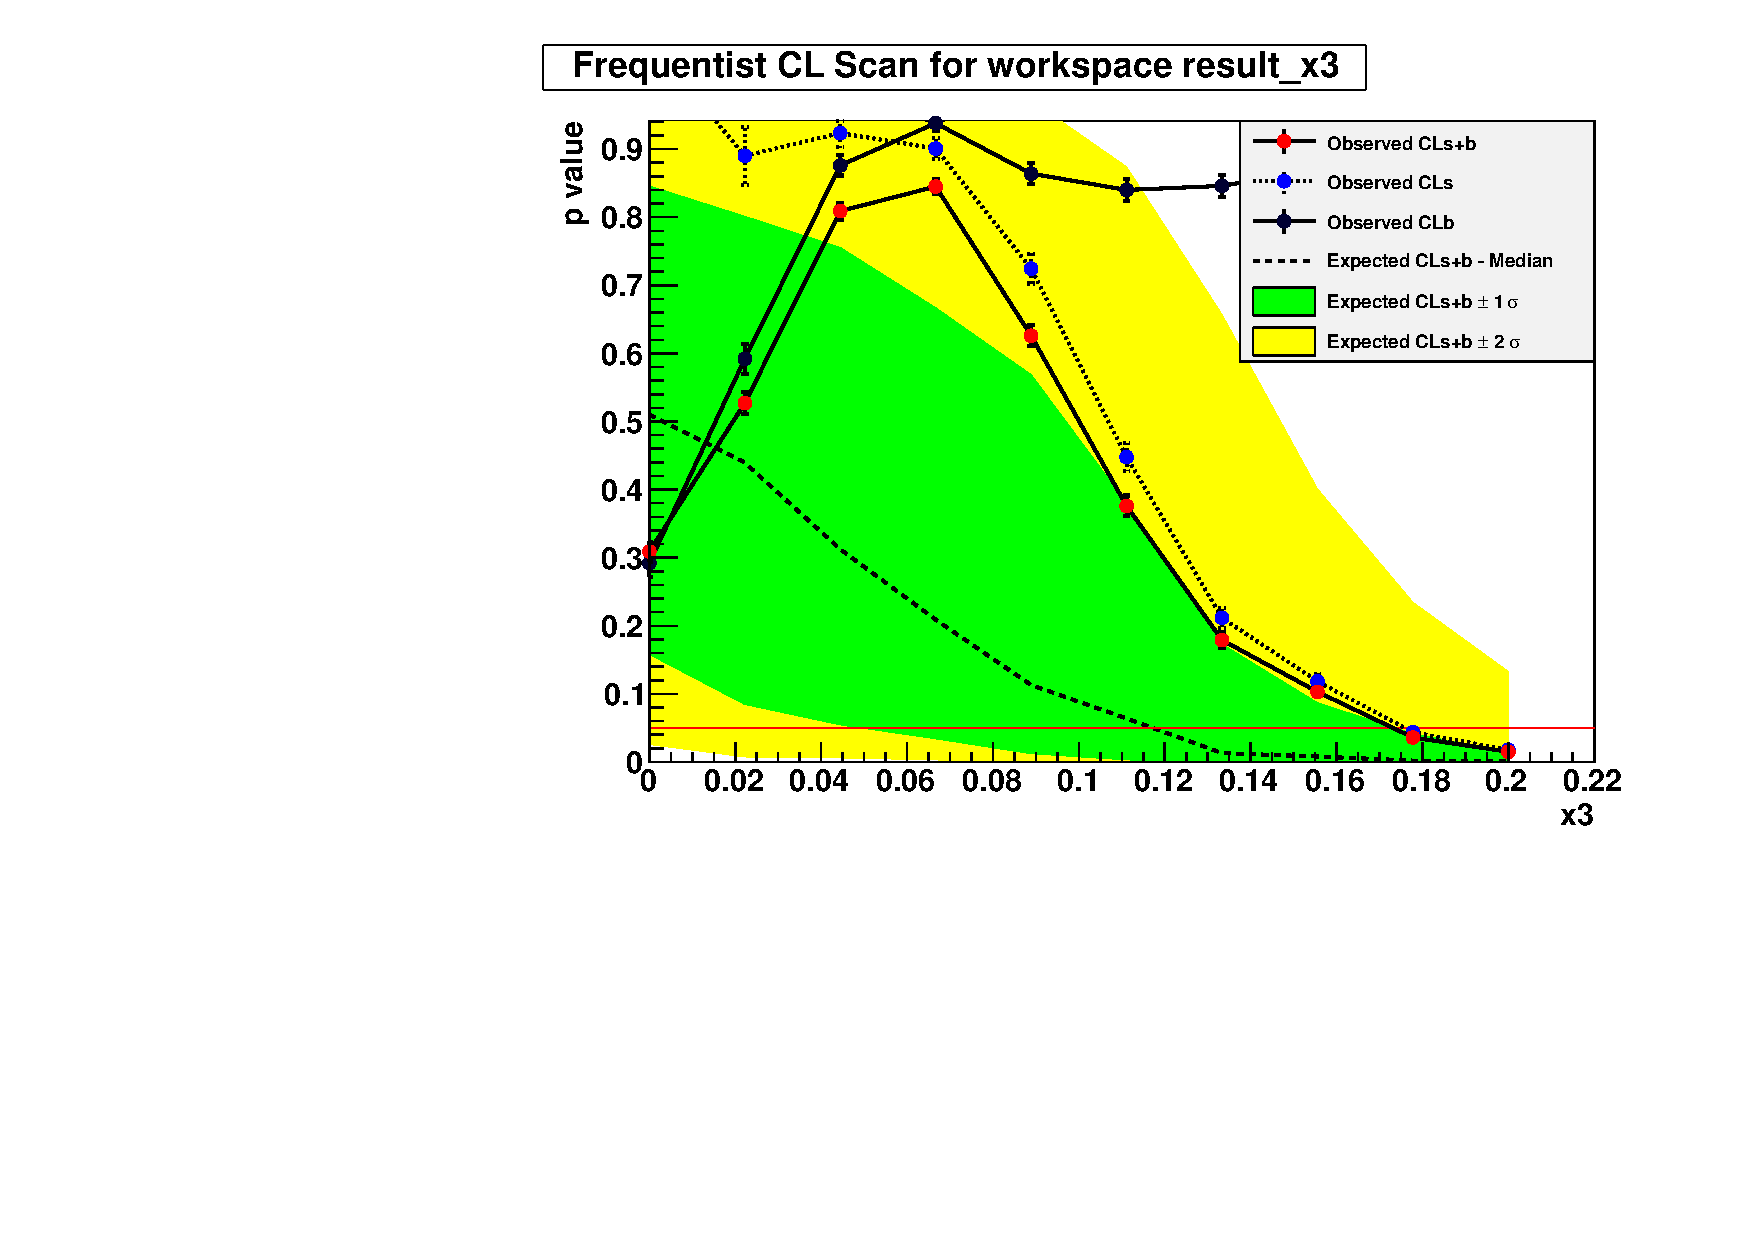
\includegraphics[angle=0,width=0.45\textwidth]{figures/limits/FC_chi3_0100.pdf}
    \caption{95\% interval on $\chi_{3}$ with Feldman Cousins technique after including systematic uncertainties. }
    \label{fig:FCx3_0100}
  \end{center}
\end{figure}


Using the profile likelihood calculator as cross-check, the 95\% C.L. interval is
$\chi_{3} \in   [0.042, 0.104]$, 
which is shown in figure \fig{fig:PLRx3_0100}.  
  

\begin{figure}[hbtp]
  \begin{center}
    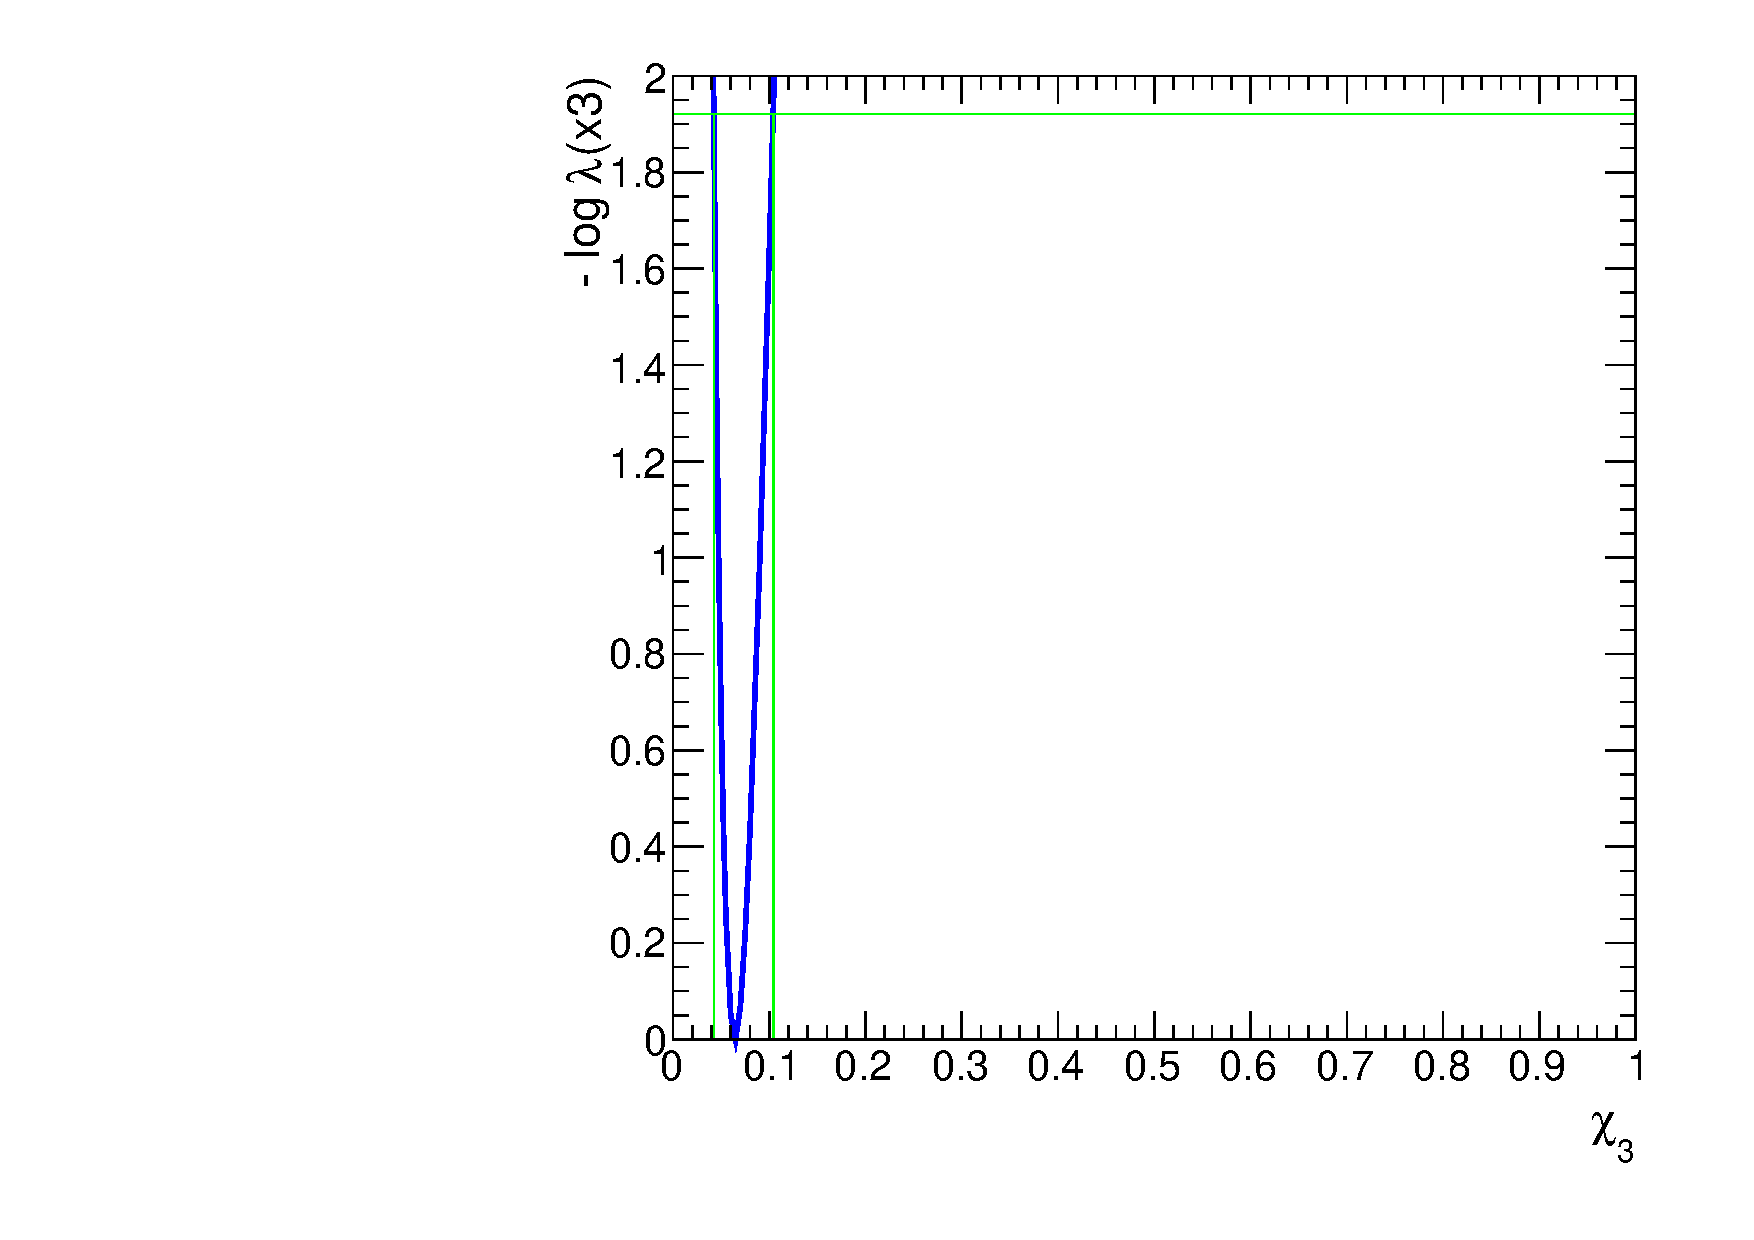
\includegraphics[angle=0,width=0.45\textwidth]{figures/limits/PLRx3_0100.pdf}
    \caption{95\% interval on $\chi_{3}$ with profile likelihood calculator not including systematic uncertainties. }
    \label{fig:PLRx3_0100}
  \end{center}
\end{figure}



Once the Raa for the $\PgUc$ signal is extracted from the simultaneous ML fit, 
we employ the Feldman-Cousins (FC) prescription to set a limit at $95\%$ confidence level~\cite{MCMC}. 
While the expected limit on the nuclear modification factor is close to a
 non-physical ($\leq 0$) result, %(i.e. $\raa(\PgUc) \leq  0$), 
the FC prescription guarantees a physically meaningful result and tells us how to smoothly 
transition from one-sided to two-sided limit. 
%The FC prescription is described in detail in Ref.~\cite{FC}. % Ref missing!
It uses a likelihood ratio as an ordering principle for selecting the acceptance
 region and creating confidence bands. The likelihood ratio is defined as the following:
\begin{equation}
Q(x)=\frac{P(x|\raa(\PgUc)_{0})}{P(x|\raa(\PgUc)_{\text{max}})} \,,
\end{equation}
where $Q(x)$ is a likelihood ratio for given $\raa(\PgUc)$, x,  a given $\raa(\PgUc)$ and finally $\raa(\PgUc)_{0}$,
and $\raa(\PgUc)_{\text{max}}$ is the $\raa(\PgUc)$ for the maximum likelihood among all possible $\raa(\PgUc)$ values.


%\subsubsection{Nuclear modification factor upper limit}
%\label{sec:raa_limits}

For the centrality-integrated bin (0 -100\%) the computed upper limit for the nuclear modification factor, $\raa(\PgUc)$, using the FC method is about 0.095 (95\% CL). This can be seen from \fig{fig:FC_Raa_Limit_MB}, when the observed $CL_s$ (red dots) crosses the horizontal threshold (red line). We generate 1000 pseudo experiments at each scanned point to discriminate the null hypothesis (no signal 3S is present) from the alternative (signal plus background) hypothesis.
%Results are summarized in Table.~\ref{tab:Raaupperlimits}. 

\begin{figure}[hbtp]
  \begin{center}
   %\subfigure[$p$-value scan using Feldman Cousins technique]{
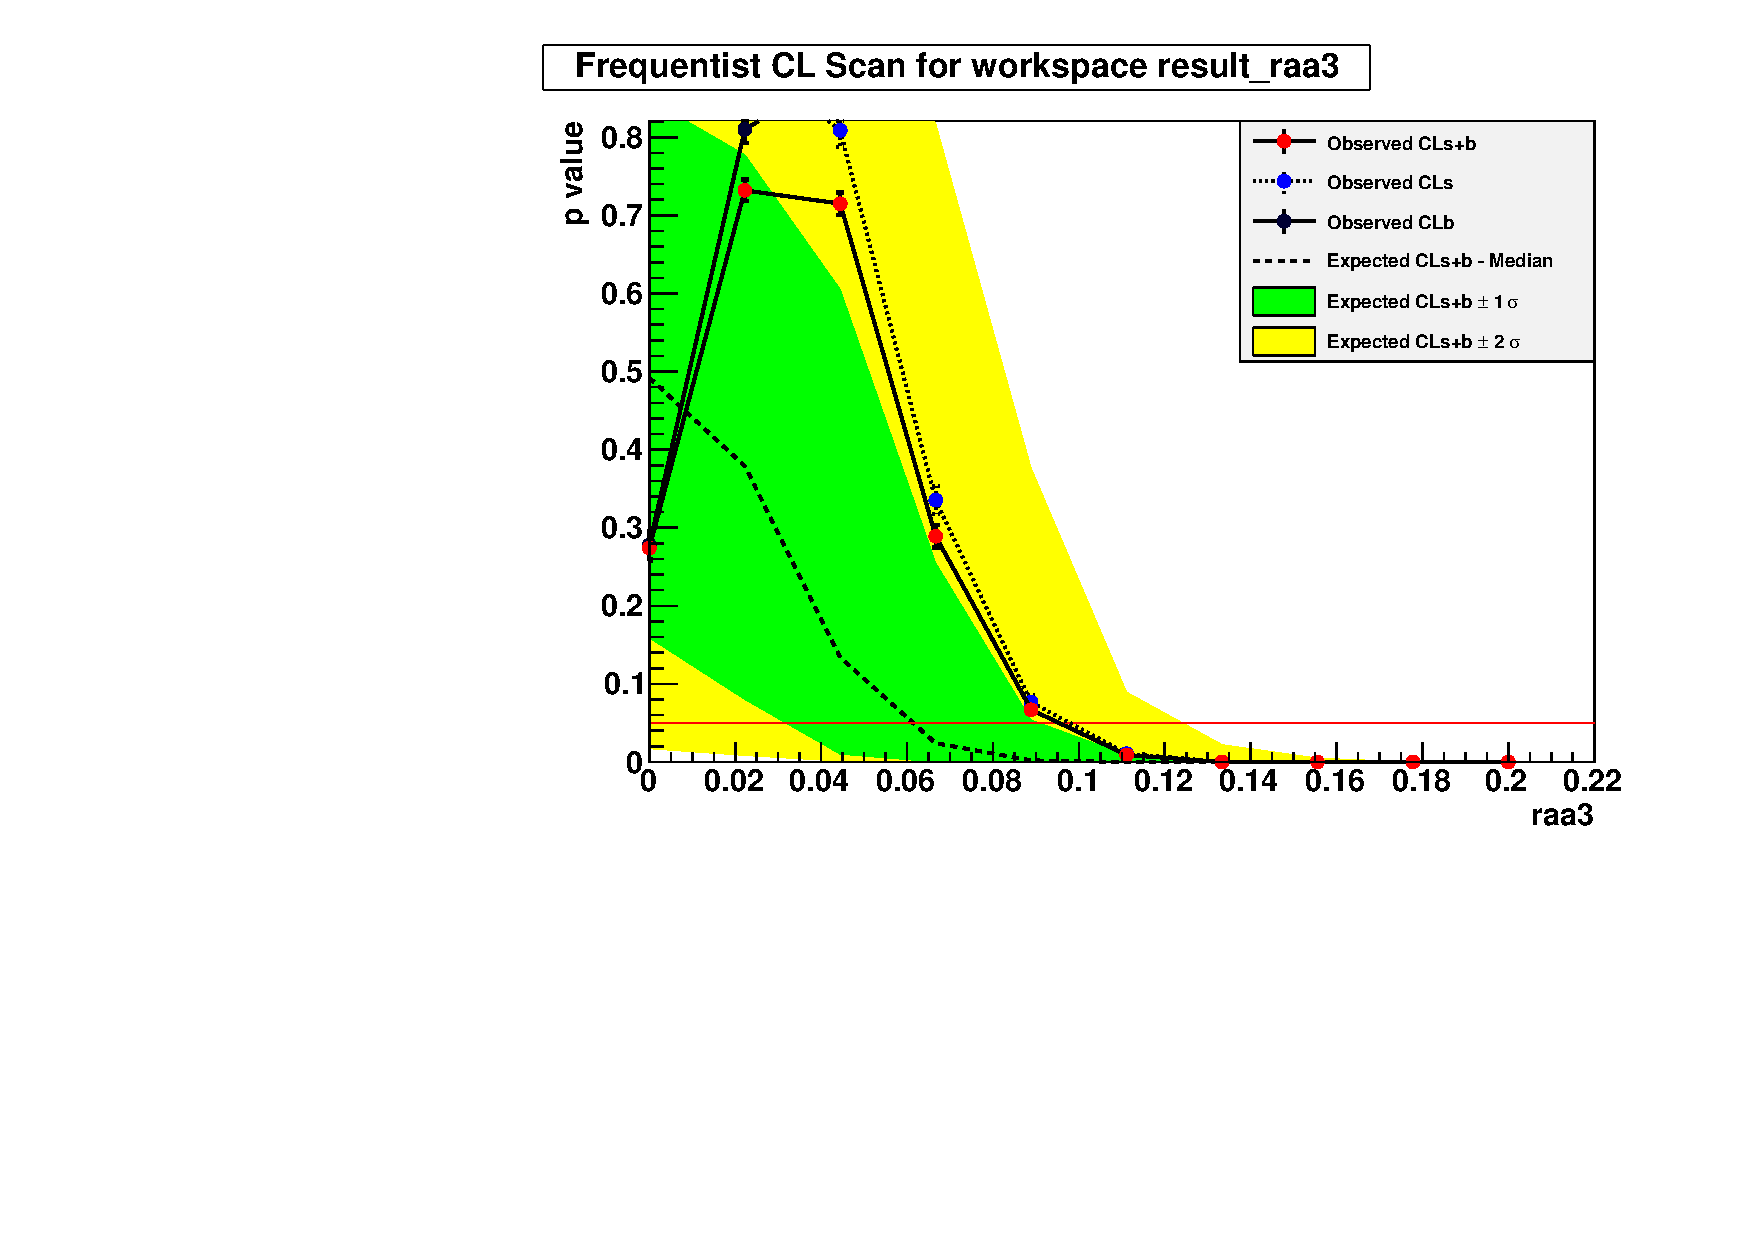
\includegraphics[angle=0,width=0.7\textwidth]{figures/limits//FC_Raa_Limit_MB}\label{fig:/FC_Raa_Limit_MB}
%}\\
   \caption{$p$-value scan for $\raa(\PgUc)$ using the Feldman-Cousins technique.}
%A thousand pseudo experiments for each of the ten points scanned. Figs~\ref{fig:/FC_Raa_Limit_MB}:Observed $CL_s$; red curve, $H_{b}$ blue curve and black line is our Test Statistics.}
   \label{fig:FC_Raa_Limit_MB}
 \end{center}
\end{figure}

\begin{figure}[hbtp]
  \begin{center}
   \subfigure[Pseudo-experiments for null and alternative hypotheses and using likelihood ratio test statistics.]{
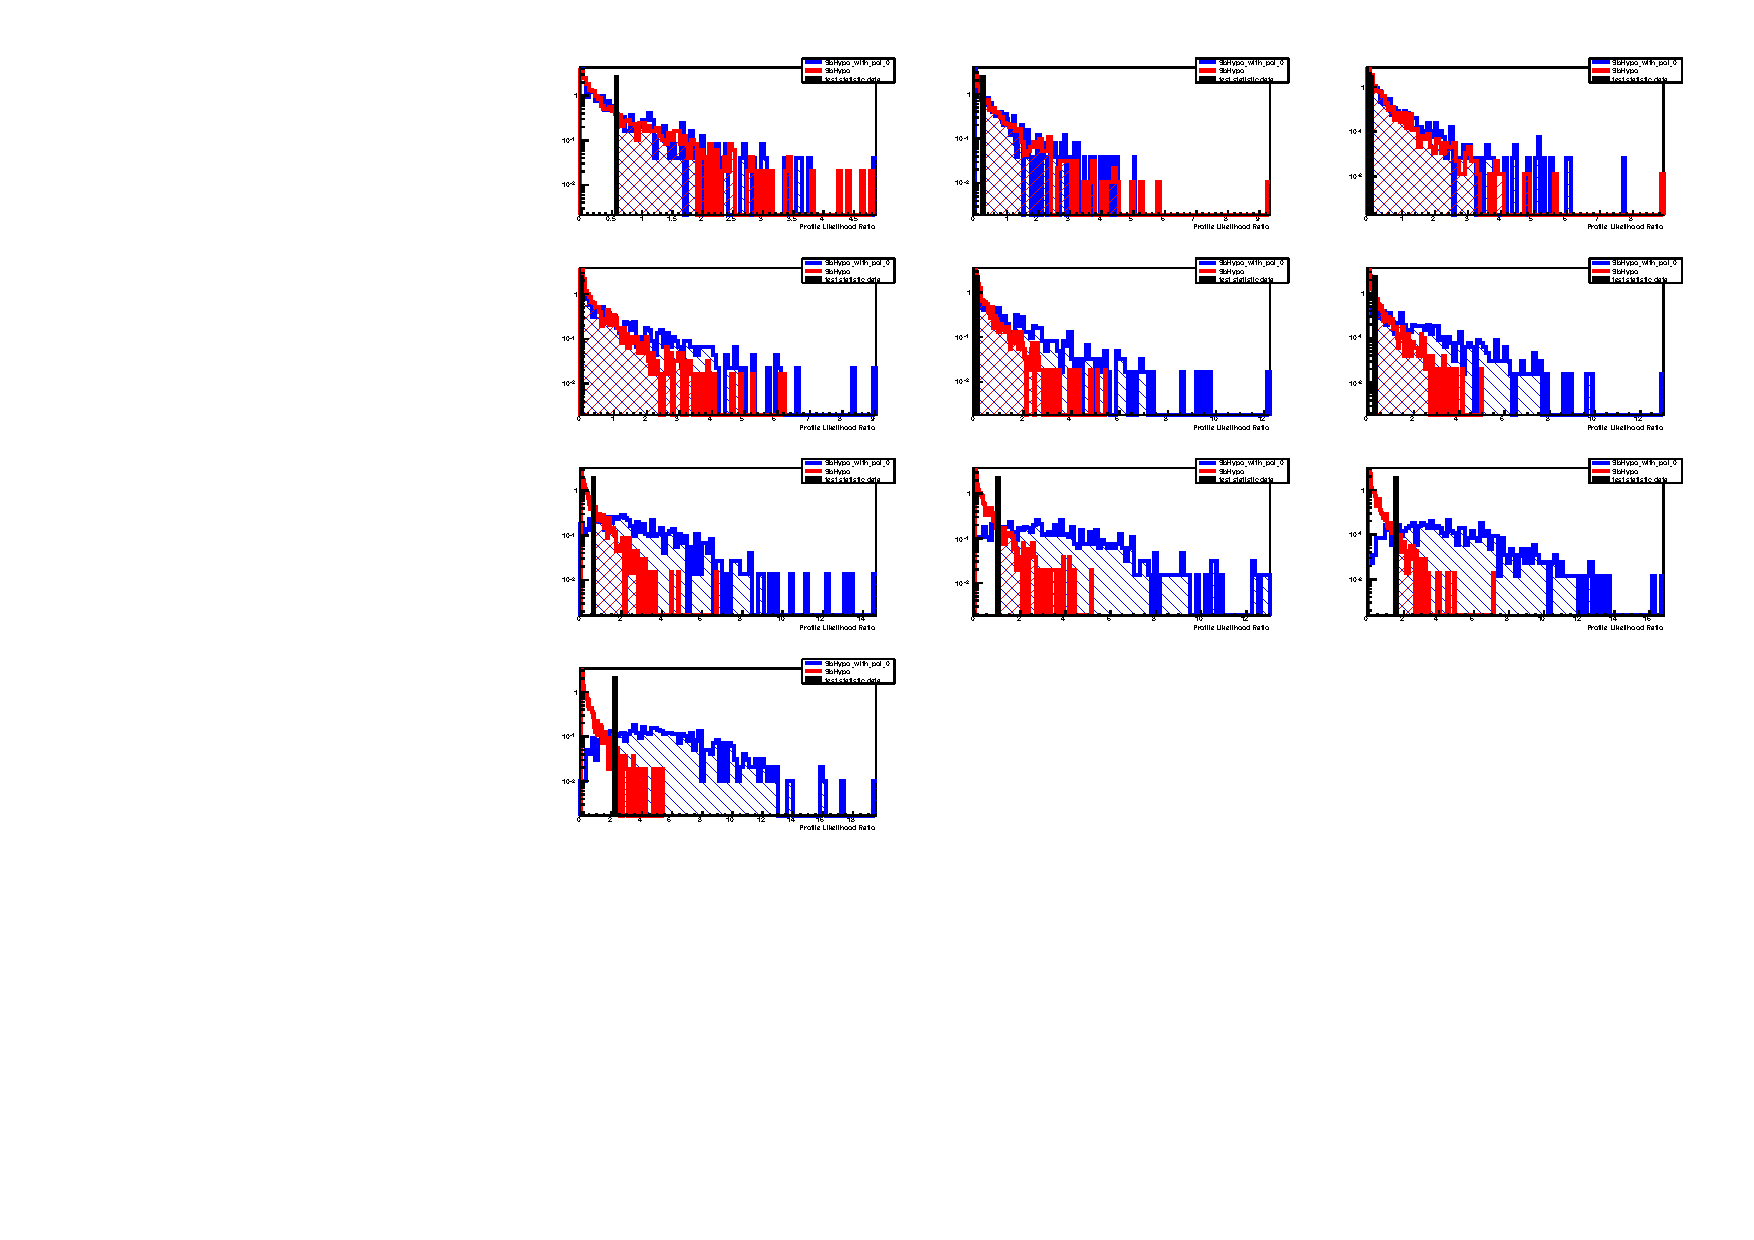
\includegraphics[angle=0,width=1.0\textwidth]{figures/limits//FCRaa3SToyswithSystematics}\label{fig:/FCRaa3SToyswithSystematics}}\\
   \caption{A thousand pseudo-experiments for each of the ten points scanned. %Figs~\ref{fig:/FCRaa3SToyswithSystematics}: 
$H_{sb}$; red curve, $H_{b}$ blue curve and black line is the test statistic. As we increase our parameter of interest it is easier to differentiate between the two hypotheses and the area under the red curve becomes smaller than the area under the blue curve.}
   \label{fig:Raatoys}
 \end{center}
\end{figure}

%\subsection{Propagation of systematic uncertainties on the limits}
%\label{sec:sysRaa}

%Because we use the reconstructed dimuon mass distributions to extract the upsilon $\raa(\PgUc)$,
%any systematic that possibly alters the shape and location of the reconstructed
%$\PgU$ mass distributions will potentially change the fitted  \raa\ out of the
%likelihood fitter. 

%\par 
The systematics uncertainties on the \pp luminosity, the nuclear overlap function $\taa$ and the efficiency ratios as well as the uncertainties for the background shape and the signal FSR need to be taken into consideration when setting the upper limit. We fold in these systematics, which were previously specified, via nuisance parameters in the fit.  
%Variation of such parameters corresponds to certain systematic uncertainties. %?..


Figure~\ref{fig:plr_Raa3S_withSystematics} %%Figure 35 %FIXME!!!!!! 
shows cross checks using the profile likelihood ratio implementation, where an $\raa(\PgUc)$ upper limit of about 0.0952 (95\% CL) is obtained. 
Notice that both results are consistent within uncertainties.  
The results for the two implementations are summarized in Table~\ref{tab:Raaupperlimits}.  

\begin{figure}[hbtp]
  \begin{center}
  % \subfigure[Pseudo Experiments for null and alternative hypotheses and using likelihood ratio test statistics]{
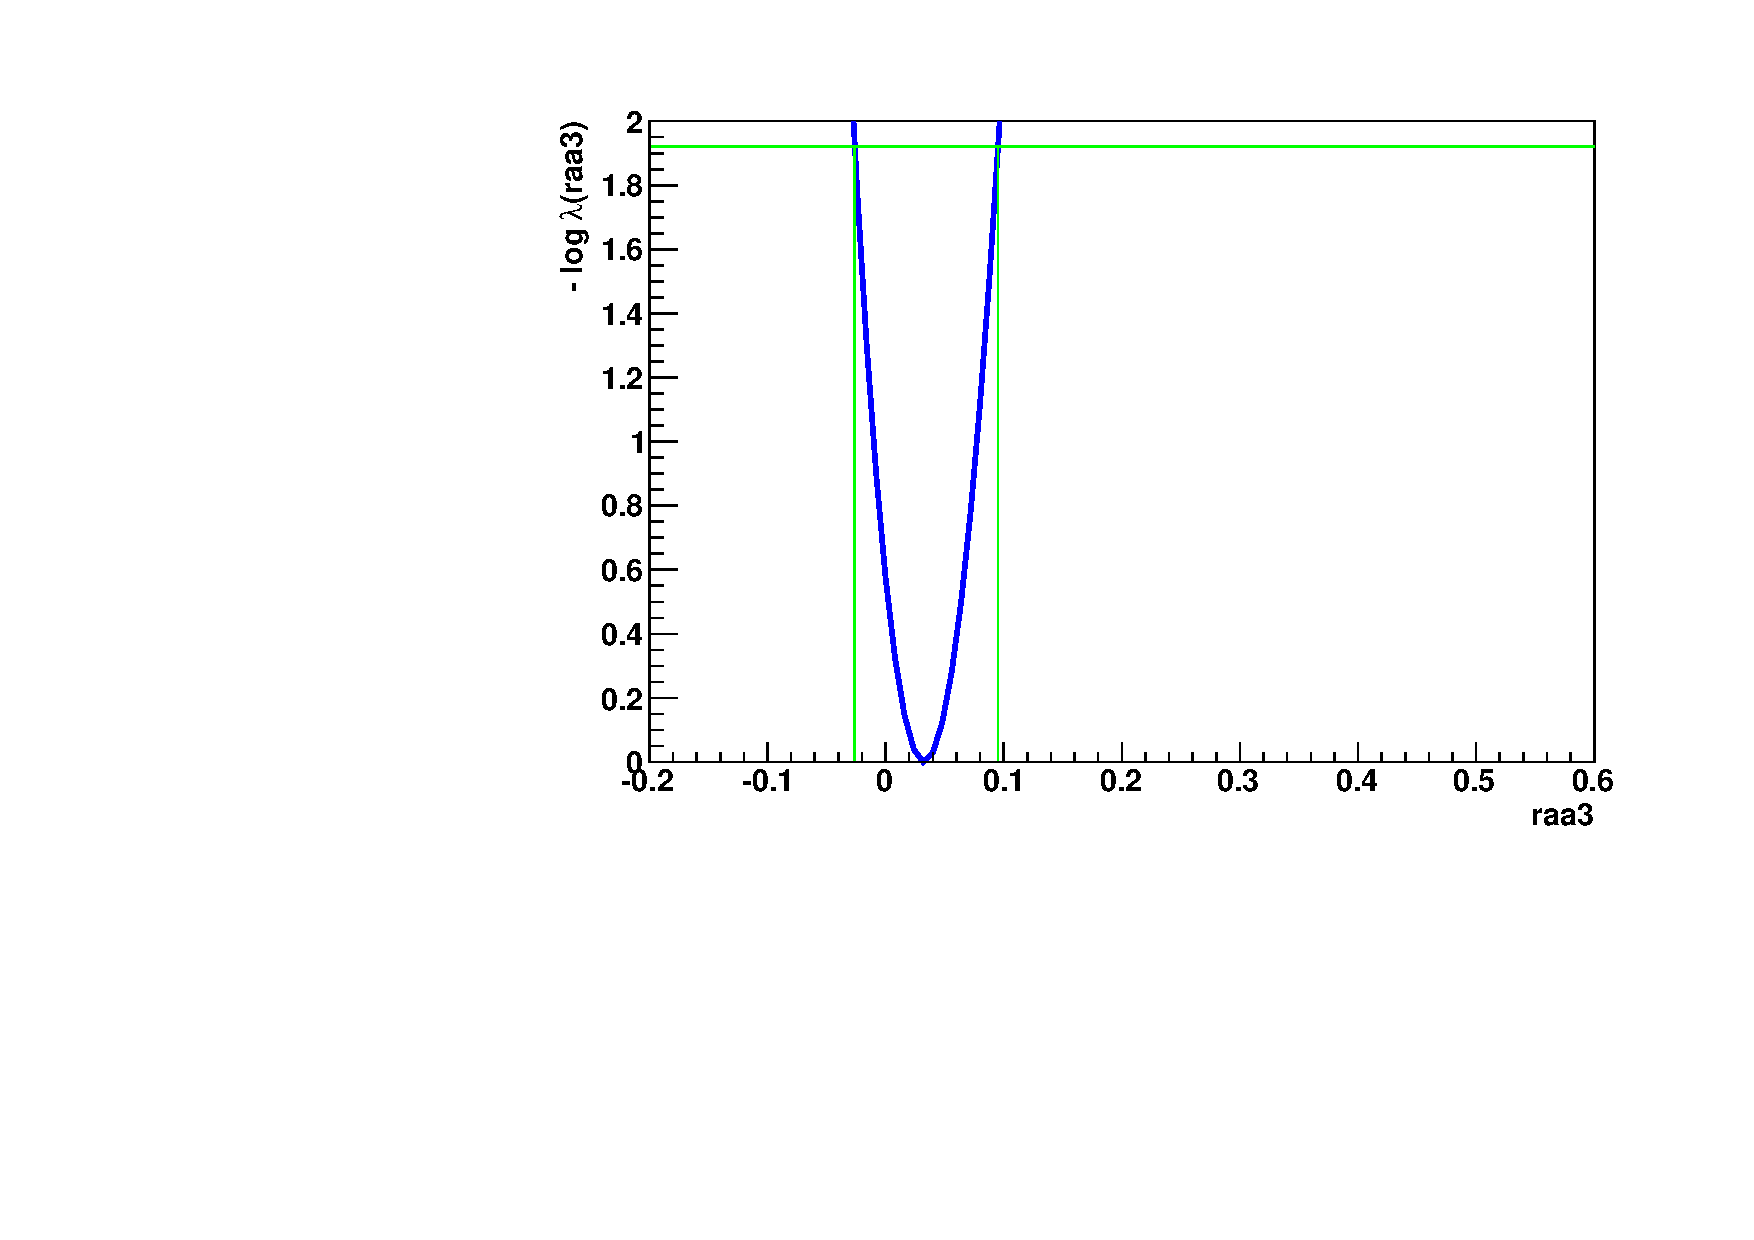
\includegraphics[angle=0,width=0.7\textwidth]{figures/limits//plr_Raa3S_withSystematics}\label{fig:/plr_Raa3S_withSystematics}
%}\\
   \caption{Profiled likelihood ratio. %Figs~\ref{fig:/plr_Raa3S_withSystematics}: 
It shows the confidence interval at $95\%$ confidence level.}
   \label{fig:plr_Raa3S_withSystematics}
 \end{center}
\end{figure}


 
\begin{table}[!v]
  \centering
  \caption{$\raa(\PgUc)$ upper limits. \emph{(Note: being updated)}}
  \begin{tabular}{c|c|c|c}
    \hline
    & & \multicolumn{2}{c}{95\% C.L upper limit}  \\
    centrality & best fit value & Feldman-Cousins & profile likelihood ratio  \\
    \hline
    0 - 100\% & $ 0.032 \pm  0.031$ &$ 0.09506 \pm 0.00130$ & $0.0952$ \\
    \hline
  \end{tabular}
  \label{tab:Raaupperlimits}
\end{table}

Since we are interested in the suppression pattern of the three $\Upsilon$ states and because the errors for the Raa for the $\Upsilon(1S)$ and $\Upsilon(2S)$ have been calculated with a 1 $\sigma$ error, we also set the upper limits at a 68\% confidence level.

In this scenario the upper limit using the Feldman Cousins technique is 

$\raa(\PgUc) \leq 0.064 \pm 0.001$  at 68\% confidence level.



\begin{figure}[hbtp]
  \begin{center}
   %\subfigure[$p$-value scan using Feldman Cousins technique at 68\% confidence level]{
\includegraphics[angle=0,width=0.7\textwidth]{figures/limits/FCRaa3S_withsystematics68}\label{fig:/FC_Raa_Limit_MB_68}
%}\\
   \caption{$p$-value scan for $\raa(\PgUc)$ using the Feldman-Cousins technique at 68 \% confidence level.}
%A thousand pseudo experiments for each of the ten points scanned. Figs~\ref{fig:/FC_Raa_Limit_MB_68}:Observed $CL_s$; red curve, $H_{b}$ blue curve and black line is our Test Statistics.}
   \label{fig:FC_Raa_Limit_MB_68}
 \end{center}
\end{figure}






We have used two Bayesian implementations to cross check our results. The first Bayesian calculation is using numeric integration assuming a flat prior to derive a one sided $95\%$ credible interval and the second one is using Markov Chain Monte Carlo sampling which is based on the Metropolis-Hastings algorithm~\cite{MCMC}. 


For the centrality integrated bin (0 -100\%) the computed upper limit for the single ratio of 3S/1S using the Feldman-Cousins method 
is $R_{3}=0.0695 \pm 0.0004$ which can be seen from \fig{fig:FC_results}. 
when the observed $CL_s$ (red dots) crosses the horizontal threshold (red line). 
In~\fig{fig:FC_Centrality} 
we present the upper limits for all the centrality bins as a function of the number of participants. The two lowest values for the upper limits were found in the centrality bins where we had negative yields from the fitted results. These upper limits are indeed positive as expected. 
Figure~\ref{fig:limits_xchecks} %%Figure 35 %FIXME!!!!!! 
shows cross checks using different implementations.  
Figs.~\ref{fig:CLs_0100} and~\ref{fig:Asmp_0100} %a) and b) %FIXME!!!!!! 
use $CL_{s}$ and its asymptotic  approximation, and 
Figs.~\ref{fig:bayesian_post_0100},~\ref{fig:bayesian_mcmc_0100} %c) and d) %FIXME!!!!!! 
use Bayesian numeric integration and Markov Chain Montecarlo, respectively. Notice that all results are consistent within uncertainties.  
Finally, %FIXME... where???
in \fig{fig:bayesian},  
 we show Bayesian results in the (30-40\%) centrality bin where we found negative ratios.
%
%The results for the various centrality bins are shown in Tables~\ref{tab:upperlimits} and~\ref{tab:credible_intervals}. 
The upper limits found for the different centrality bins are tabulated in Tables~\ref{tab:upperlimits} and~\ref{tab:credible_intervals}. 

%FIXME: PLOTS ARE NOT REFERENCED/EXPLAINED IN THE TEXT

\begin{figure}[hbtp]
  \begin{center}
    %\subfigure[Upper limits for all centrality bins.]
{\includegraphics[angle=0,width=0.45\textwidth]{figures/limits/FC_Centrality}\label{fig:FC_Centrality}}
   \caption{Upper limit results using the Feldman-Cousins method on $R_3$ in \PbPb, evaluated for the different centrality bins. \emph{(Note: being updated)}
}
    \label{fig:FC_Centrality}
  \end{center}
\end{figure}


\begin{figure}[hbtp]
  \begin{center}
    \subfigure[Observed CLs crosses the 0.05 red line]{\includegraphics[angle=0,width=0.5\textwidth]{figures/limits/Cls_0100}\label{fig:CLs_0100}}
    \subfigure[Asymptotic approach using Asimov test statistics]{\includegraphics[angle=0,width=0.4\textwidth]{figures/limits/Asymptotic_0100}\label{fig:Asmp_0100}}\\
    \subfigure[Bayesian posterior]{\includegraphics[angle=0,width=0.5\textwidth]{figures/limits/bayesian_num_posterior_0100}\label{fig:bayesian_post_0100}}
    \subfigure[Markov Chain Montecarlo]{\includegraphics[angle=0,width=0.5\textwidth]{figures/limits/bayesian_mcmc_posterior_0100}\label{fig:bayesian_mcmc_0100}}
    \caption{CLs and Bayesian cross checks for the centrality integrated bin, using uniform prior. Figs~\ref{fig:CLs_0100},~\ref{fig:Asmp_0100}: p-value Scan with different test statistics using 1000 pseudo experiments at each point; Figs~\ref{fig:bayesian_post_0100},~\ref{fig:bayesian_mcmc_0100}: Two different Bayesian approaches: Numerical calculation and Markov Chain Monte Carlo. \emph{(Note: being updated)}}
    \label{fig:limits_xchecks}
  \end{center}
\end{figure}



\begin{figure}[hbtp]
  \begin{center}
    \subfigure[Bayesian posterior]{\includegraphics[angle=0,width=0.5\textwidth]{figures/limits/bayesian_num_posterior_3040}\label{fig:bayesian_post_3040}}
%   \subfigure[Markov Chain MonteCarlo steps]{\includegraphics[angle=0,width=0.5\textwidth]{figures/limits/scatter_mcmc_f3_vs_beta_nbkg_3040_lores}\label{fig:scatter_mcmc}} 
    \subfigure[MC Markov Chain posterior]{\includegraphics[angle=0,width=0.5\textwidth]{figures/limits/bayesian_mcmc_posterior_3040}\label{fig:bayesian_mcmc_3040}}
    \caption{Bayesian results for 40-50\% centrality bin. Figures~\ref{fig:bayesian_post_3040},~\ref{fig:bayesian_mcmc_3040}: Bayesian Numeric Calculator and Montecarlo Markov Chain. % ; Figs~\ref{fig:scatter_mcmc}: Number of steps in chain: 26701.
\emph{(Note: being updated)}
}
    \label{fig:bayesian}
  \end{center}
\end{figure}

%\begin{figure}[hbtp]
%  \begin{center}
%    \subfigure[Pseudo Experiments for null and alternative hypotheses and test statistics]{\includegraphics[angle=0,width=1.0\textwidth]{figures/limits/FC_toys_0100}\label{fig:FC_toys_0100}}\\
%    \caption{A thousand pseudo experiments for each of the ten points scanned. Figs~\ref{fig:FC_toys_0100}:$ H_{sb}$; red curve, $H_{b}$ blue curve and black line is our Test Statistics}
%    \label{fig:toys}
%  \end{center}
%\end{figure}


 
\begin{table}[!v]
  \centering
  \caption{Single-ratio upper limits. \emph{(Note: being updated)}}
  \begin{tabular}{c|c|c|c|c}
    \hline
    & $R_{3} $ & Feldman-Cousins & frequentist scan $CL_{s}$ & asymptotic scan \\
    \hline
    0 - 5\%   & $0.043 \pm 0.051$ & $ 0.147 \pm 0.003$ & $0.143 \pm 0.005$ & $0.129$ \\
    5 - 10\% & $0.018 \pm 0.055$ & $0.1368 \pm 0.0009$ & $0.2222 \pm 0.0002$ & $0.124$ \\
    10 - 20\% & $0.0062 \pm  0.0352$ & $0.1390 \pm 0.0009$ & $0.3129 \pm 0.0005$ & $0.074$ \\
    20 - 30\% & $0.052 \pm 0.036$ & $0.1232 \pm 0.0006 $ & $0.110 \pm 0.0003$ & $0.11$ \\
    30 - 40\% & $-0.046 \pm 0.045$ & $0.0407 \pm 0.0001$ & $0.065 \pm 0.011$ & $0.063$ \\
    40 - 50\% & $0.23 \pm 0.070$ &$ 0.0980 \pm 0.0003$ & $0.364 \pm 0.003$ & $0.35$\\
    50 - 100\% & $ -0.069 \pm 0.061 $ & $0.054 \pm 0.0002$ & $0.081 \pm 0.005 $ & $0.084$\\
    \hline
    0 - 100\% & $0.032 \pm 0.019$ & $0.0695 \pm 0.0004$ & $0.0638 \pm 0.00006$ & $0.0631$\\
    \hline
  \end{tabular}
  \label{tab:upperlimits}
\end{table}

\begin{table}[!v]
  \centering
  \caption{Single-ratio credible intervals: Bayesian cross checks. \emph{(Note: being updated)}}
  \begin{tabular}{c|c|c|c}
    \hline
    & $R{3} $ & Bayesian calculator & $MCMC$  \\
    \hline
    0 - 5\%   & $0.043 \pm 0.051$ & $[-1, 0.12]$ & $[-1, 0.14]$\\
    5 - 10\% & $0.018 \pm 0.055$  & $[-1, 0.091]$ & $ [-1, 0.47]$\\
    10 - 20\% & $0.0062 \pm  0.0352$  & $[-1, 0.051]$ & $[-1, 0.070]$\\
    20 - 30\% & $0.052 \pm 0.036$ & $[-1, 0.091]$ & $[-1, 0.11]$\\
    30 - 40\% & $-0.046 \pm 0.045$ & $[-1, 0.010]$ & $[-1, 0.028]$\\
    40 - 50\% & $0.23 \pm 0.070$ & $[-1, 0.33]$ & $[-1, 0.41]$\\
    50 - 100\% & $ -0.069 \pm 0.061 $ & $ [-1, 0.010]$ & $[-1, 0.062]$  \\
    \hline    
    0 - 100\% & $0.032 \pm 0.019$& $[-1, 0.051]$ & $[-1, 0.062]$\\
    \hline
  \end{tabular}
  \label{tab:credible_intervals}
\end{table}

\end{chapter}

%\include{Chapter9}

\chapter{Final results}
Bottomonium suppression in PbPb collisions is studied in this section by measuring the ratios of observed yields of excited $\PgU$ states relative to the ground $\PgUa$ state, with the $150 \mu b^{-1}$ 2011 \PbPb\ data. The suppression is inferred by performing a comparison of the ratios measured in PbPb against the \pp\ reference. Dependencies on the centrality of the  \PbPb collision are explored. 

The data samples,  reconstruction and selection criteria are described in Sections~\ref{sec:datasets} and~\ref{sec:selection}. 
%
The parameters of interest are extracted from the data samples directly via an extended unbinned maximum likelihood fit to the dimuon invariant-mass spectra, described in Section~\ref{sec:fitting}.


\subsection{Single ratio measurement}
\label{sec:singleratio}

The following ratios of observed yields of $\PgU$ excited states relative to the ground state are studied:
%
\begin{linenomath}
\begin{eqnarray}
\label{eqn:def:r23}
R_{23} & \equiv & \frac{N\left(\PgUb+\PgUc\right)}{N(\PgUa)} \,,\\
\label{eqn:def:r2}
R_{2}  & \equiv & \frac{N\left(\PgUb      \right)}{N(\PgUa)} \,, \\
\label{eqn:def:r3}
R_{3}  & \equiv & \frac{N\left(\PgUc      \right)}{N(\PgUa)} \,.
\end{eqnarray}
\end{linenomath}
%
In addition to the combined excited-to-ground ratio, $R_{23}$, the current statistics allow to extract the separate 2S and 3S ratios, $R_{2}$ and $R_3$. 
No evidence for the $\PgUc$ state is found in the \PbPb data, and the corresponding ratio is studied in Sec.~\ref{sec:limits}. 

These ratios are measured from fits to the PbPb and \Pp\Pp{} datasets, separately performed. 
The nominal $\pt>4.0 \GeVc$ cut is used.
%\footnote{Fit results with $\pt>3.5 \GeVc$ single-muon cut are collected in Appendix~\ref{sec:newdata150}.}
These fits are displayed in \fig{fig:final_massfit_nominal}.
%{fig:massfit_singlerat_pbpb_nominal} and~\ref{fig:massfit_singlerat_pp_nominal}. 
The fit results are shown in Table~\ref{tab:single-rat} for the PbPb data, and in Table~\ref{tab:single-rat-pp} for the \pp\ (2.76 TeV) dataset. 

\begin{figure}[hbtp]
  \begin{center}
    \subfigure[Fit to the PbPb data]{\includegraphics[angle=0,width=0.5\textwidth]{figures/fulldataset/masspeak_Hi_paramOn.pdf}\label{fig:final_massfit_PbPb}}
    \subfigure[Fit to the pp data]{\includegraphics[angle=0,width=0.5\textwidth]{figures/fulldataset/masspeak_pp_HIrereco_pol2_fix_paramOn.pdf}\label{fig:final_massfit_pp}} \\
  \caption{Nominal mass fits, performed separately to the \PbPb ($150 \mu b^{-1}$)  and \pp ($231 nb^{-1}$) full datasets.}
  \label{fig:final_massfit_nominal}
  \end{center}
\end{figure}


Various systematic variations of the fit model are performed, to further establish the stability of the results. 
For the fit to the PbPb data, the following variations are considered:
\begin{itemize}
\item like-sign background modeling: the background model is formed of two components, given by the like-sign distribution and a second order polynomial; the PDF from the like-sign data is obtained from a fit employing the erf * exp model (Fig~\ref{fig:final_PbPb_LSerf}) 
\item like-sign background modeling: the background model is formed of two components, given by the like-sign distribution and a second order polynomial; the PDF from the like-sign data is obtained from the RooKeysPdf smoothing method (Fig~\ref{fig:final_PbPb_LSkeys})
%\item narrow range mass fit (8.5 -- 14 \GeVcc), fitted with second order polynomial (Fig~\ref{fig:final_PbPb_pol2})
%\item narrow range mass fit (8.5 -- 14 \GeVcc), fitted with  first order polynomial (Fig~\ref{fig:final_PbPb_pol1})
\item track-rotation background modeling: the background model is formed of two components, given by the track-rotation distribution and a second order polynomial; the PDF from the track-rotation data is obtained from a fit employing the erf * exp model (Fig~\ref{fig:final_PbPb_TRerf} and~\ref{fig:final_PbPb_TRerf_OS})
\item track-rotation background modeling: the background model is formed of two components, given by the track-rotation distribution and a second order polynomial; the PDF from the track-rotation data is obtained from the RooKeysPdf smoothing method (Fig~\ref{fig:final_PbPb_TRkeys} and~\ref{fig:final_PbPb_TRkeys_OS})
\item the CB signal tail parameters are fixed ($\alpha=1.4$, from high-statistics $\Pp\Pp$ data as in Table~\ref{tab:fsr}) (Fig~\ref{fig:final_PbPb_CBfix}) %, $\sigma_{1S}=92\MeVcc)$
\item the resolution is fixed ($\sigma_{1S}=92\MeVcc$) (Fig~\ref{fig:final_PbPb_resolfix})
%\item wide range mass fit (6 -- 15 \GeVcc), using nominal model (this variations is provided only as a check, given below 7\GeVcc the background model does not provide an appropriate discription of the data)
\item the signal shape parameters are fixed ($\alpha=1.4$, $n=2.3$, $\sigma_{1S}=92\MeVcc$) (Fig~\ref{fig:final_PbPb_CBresolfix})
\end{itemize}

For the fit to the pp data, these variations are considered:
\begin{itemize}
\item the CB signal tail parameters are fixed ($\alpha=1.4$, from high-statistics $\Pp\Pp$ data as in Table~\ref{tab:fsr})  %, $\sigma_{1S}=92\MeVcc)$
\item the resolution is fixed ($\sigma_{1S}=92\MeVcc$) 
\item the signal shape parameters are fixed ($\alpha=1.4$, $n=2.3$, $\sigma_{1S}=92\MeVcc$) 
\item like-sign background modeling: the background model is formed of two components, given by the like-sign distribution and a second order polynomial; the PDF from the like-sign data is obtained from a fit employing the erf * exp model
\item like-sign background modeling: the background model is formed of two components, given by the like-sign distribution and a second order polynomial; the PDF from the like-sign data is obtained from the RooKeysPdf smoothing method
\item error function for background shape
\end{itemize}
%
%For each case, the largest variation observed is assigned as the systematic uncertainty on the measurement. 

\begin{figure}[hbtp]
  \begin{center}
    \subfigure[fix CB to MC (alpha = 1.4)]{\includegraphics[angle=0,width=0.3\textwidth]{figures/fulldataset/masspeak_hi_CBfix.pdf}\label{fig:final_PbPb_CBfix}}
    \subfigure[fix resolution to MC]{\includegraphics[angle=0,width=0.3\textwidth]{figures/fulldataset/masspeak_hi_resol_fix.pdf}\label{fig:final_PbPb_resolfix}}
    \subfigure[fix CB and resolution to MC]{\includegraphics[angle=0,width=0.3\textwidth]{figures/fulldataset/masspeak_hi_resolCB_fix.pdf}\label{fig:final_PbPb_CBresolfix}}\\ 
    \subfigure[LS keys + pol2]{\includegraphics[angle=0,width=0.3\textwidth]{figures/fulldataset/masspeak_hi_LSkeys.pdf}\label{fig:final_PbPb_LSkeys}}
    \subfigure[LS TrkRot keys + pol2]{\includegraphics[angle=0,width=0.3\textwidth]{figures/fulldataset/masspeak_hi_TRkeys.pdf}\label{fig:final_PbPb_TRkeys}}
    \subfigure[OS TrkRot keys + pol2]{\includegraphics[angle=0,width=0.3\textwidth]{figures/fulldataset/masspeak_Hi_keysPdf_OS_trkRot.pdf}\label{fig:final_PbPb_TRkeys_OS}}\\
    \subfigure[LS erf*exp + pol2]{\includegraphics[angle=0,width=0.3\textwidth]{figures/fulldataset/masspeak_hi_LSerf.pdf}\label{fig:final_PbPb_LSerf}}
    \subfigure[LS TrkRot erf*exp + pol2]{\includegraphics[angle=0,width=0.3\textwidth]{figures/fulldataset/masspeak_hi_TRerf.pdf}\label{fig:final_PbPb_TRerf}}
    \subfigure[OS TrkRot erf*exp + pol2]{\includegraphics[angle=0,width=0.3\textwidth]{figures/fulldataset/masspeak_Hi_paramOn_OS_trkRot.pdf}\label{fig:final_PbPb_TRerf_OS}}
  \caption{PbPb fit model variations ($150 \mu b^{-1}$).}
  \label{fig:PbPb_model_variations}
  \end{center}
\end{figure}

The associated systematic uncertainties are summarized in Table~\ref{tab:final-single-rat} for \PbPb, and in Table~\ref{tab:final-single-rat-pp} for \pp.  
%
From the several variations, two estimates of the systematic uncertainty are provided: 
(i) the quadratic-mean deviation relative to the nominal central value, RMS (schematically, $\sqrt{(\sum{\text{variation - nominal})^2} / (n-1)}$); and (ii) the largest deviation. 
The latter is used as the estimated systematic uncertainty.

\begin{table}[!h]
  \centering
  \caption{Summary of single-ratio results, for the PbPb dataset.}
  \begin{tabular}{l|c|c|c}
    \hline
 &\multicolumn{3}{|c}{$\pt^\mu>4\GeVc$, Cent. 0-100\%}\\
 &\multicolumn{1}{|c}{$R_{23}$}& \multicolumn{1}{|c}{$R_{2}$} & \multicolumn{1}{|c}{$R_{3}$} \\
\hline
nominal (erf*exp)                   & $0.155\pm 0.038$ & $0.127\pm 0.027$ & $0.027\pm0.025$ \\
\hline
 \multicolumn{4}{l}{systematic variations:} \\
like-sign (LS) keyspdf + pol.2      & $0.159\pm 0.037$ & $0.130\pm 0.027$ &  $0.029\pm0.046 $  \\
LS erf*exp + pol.2                  & $0.151\pm 0.038$ & $0.124\pm 0.027$ &  $0.027\pm0.047 $   \\
%LS Track Rotation (TR) keyspdf + pol.2 & $0.170\pm 0.036$ & $0.137\pm 0.026$ &  $0.033\pm0.044 $  \\
%LS TR erf*exp + pol.2               & $0.159\pm 0.038$ & $0.129\pm 0.027$ &  $0.030\pm0.047 $   \\  
opposite-sign (OS) Track Rotation (TR) keyspdf + pol.2 & $0.157\pm 0.037$ & $0.120\pm 0.027$ &  $0.037\pm0.046 $  \\
OS TR erf*exp + pol.2               & $0.152\pm 0.037$ & $0.125\pm 0.027$ &  $0.025\pm0.046 $   \\
fix CB tail from MC (alpha = 1.4)   & $0.130\pm 0.038$ & $0.113\pm 0.027$ &  $0.017\pm0.047 $   \\
fix resolution from MC (92 \MeVcc)  & $0.159\pm 0.038$ & $0.128\pm 0.028$ &  $0.031\pm0.047 $  \\
fix both CB and resolution from MC  & $0.140\pm 0.037$ & $0.118\pm 0.027$ &  $0.022\pm0.046 $  \\
\hline
fit systematic (RMS)              & 0.011 & 0.007 & 0.005  \\
fit systematic (largest variation)& 0.026 & 0.016 & 0.015  \\
\hline
 \multicolumn{4}{l}{other checks:} \\
%opposite-sign (OS) TR keyspdf + pol.2 & $0.157\pm 0.037$ & $0.120\pm 0.027$ &  $0.037\pm0.046 $  \\ 
%OS TR erf*exp + pol.2               & $0.152\pm 0.037$ & $0.125\pm 0.027$ &  $0.025\pm0.046 $   \\ 
LS Track Rotation (TR) keyspdf + pol.2 & $0.170\pm 0.036$ & $0.137\pm 0.026$ &  $0.033\pm0.044 $  \\
LS TR erf*exp + pol.2               & $0.159\pm 0.038$ & $0.129\pm 0.027$ &  $0.030\pm0.047 $   \\
\hline
nominal simultaneous fit (erf*exp)  & $0.143\pm 0.038$ & $0.119\pm 0.027$ & $0.024\pm0.024$ \\
\hline
%efficiency systematic             & 4.6\% & 4.6\% & 4.6\%  \\
%\hline
%total systematic                  & 0.015 & 0.010 & 0.005 \\
%\hline
  \end{tabular}
  \label{tab:final-single-rat}
\end{table}

\begin{table}[!h]
  \centering
  \caption{Summary of single-ratio results for the \Pp\Pp{} 2.76 TeV dataset.}
  \begin{tabular}{l|c|c|c}
    \hline
 &\multicolumn{3}{|c}{$\pt^\mu>4\GeVc$}\\ 
 &\multicolumn{1}{|c}{$R_{23}$}& \multicolumn{1}{|c}{$R_{2}$} & \multicolumn{1}{|c}{$R_{3}$} \\  
\hline
nominal (pol2; signal pdf fixed from PbPb)    & $0.88\pm 0.17$ & $0.50\pm 0.12$ & $0.38\pm 0.10$ \\
\hline
 \multicolumn{4}{l}{systematic variations:} \\
fix CB tail from MC                      & $0.85\pm 0.16$ & $0.49\pm 0.11$ & $0.36\pm0.19 $  \\
fix resolution from MC                   & $0.89\pm 0.16$ & $0.49\pm 0.12$ & $0.40\pm0.20 $  \\
fix both CB and resolution               & $0.87\pm 0.16$ & $0.49\pm 0.11$ & $0.38\pm0.19 $  \\
erf*exp                                  & $0.86\pm 0.16$ & $0.49\pm 0.11$ & $0.37\pm0.19 $   \\  
LS keyspdf + pol.2                       & $0.84\pm 0.17$ & $0.48\pm 0.12$ & $0.36\pm0.21 $   \\  
LS erf*exp + pol.2                       & $0.87\pm 0.16$ & $0.49\pm 0.12$ & $0.38\pm0.20 $   \\  
\hline
fit systematic (RMS)               & 0.023 & 0.012 & 0.015  \\  
fit systematic (largest variation) & 0.051 & 0.024 & 0.035  \\
\hline
nominal simultaneous fit (pol2)  & $0.97\pm 0.19$ & $0.56\pm 0.13$ & $0.41\pm0.11$ \\
\hline
%efficiency systematic              & 6.2\% & 6.2\% & 6.2\%  \\
%\hline
%total systematic                   & 0.059 & 0.033 & 0.028  \\
%\hline
  \end{tabular}
  \label{tab:final-single-rat-pp}
\end{table}


\subsection{Centrality dependence}

Effects induced by the hot medium are expected to display, in general, a dependence on the centrality of the collision -- the effect is more accentuated for the most central collision events, and approaching the most peripheral events tend asymptotically towards the results expected in the absence of medium effects. 
%The pp collision results are usually %is sometimes
% taken as reference for the un-modified case. 
%Such basic behaviour can nonetheless be challenged, as a consequence of complexity of the underlying phenomena.  
%
The \pp collision results are taken as reference for absence of nuclear effects. 
%for the un-modified case. 

We repeat the single ratio measurement, by splitting the PbPb dataset in ranges of the collision centrality. 
The mass fit results are shown in Figures~\ref{fig:final_massfit_singlerat_centrality}.

The systematic uncertainties are evaluated for the nominal selection, and summarized in Table~\ref{tab:final_singlerat_centrality}. The corresponding differential results are displayed in \fig{fig:final_singlerat_centrality_nominal}. In these plots, the single ratio values are normalized by the central value of the measurement performed using the \Pp\Pp{} data. Note these normalization values depend on the \pt{} threshold case, and are obtained from the fit to the \Pp\Pp{} data with constrained signal shape from MC, displayed in Table~\ref{tab:final-single-rat-pp}. 
 Uncertainties on the single-point \Pp\Pp~measurement are not included, as such common uncertainty factor is not relevant for point-to-point comparison in this plot showing the double ratio trend with $N_{part}$. Some error bars in \fig{fig:final_singlerat_centrality_nominal} reach negative values, so we refine this using Feldman-Cousins limit calculation as shown in \fig{fig:final_singlerat_centrality_limit}. 

 
\begin{figure}[hbtp]
  \begin{center}
\subfigure[ 0-  5\%]{\includegraphics[angle=0,width=0.3\textwidth]{figures/fulldataset/masspeak_Hi_paramOn_cntr0-5}}
\subfigure[ 5- 10\%]{\includegraphics[angle=0,width=0.3\textwidth]{figures/fulldataset/masspeak_Hi_paramOn_cntr5-10}}
\subfigure[10- 20\%]{\includegraphics[angle=0,width=0.3\textwidth]{figures/fulldataset/masspeak_Hi_paramOn_cntr10-20}}\\
\subfigure[20- 30\%]{\includegraphics[angle=0,width=0.3\textwidth]{figures/fulldataset/masspeak_Hi_paramOn_cntr20-30}}
\subfigure[30- 40\%]{\includegraphics[angle=0,width=0.3\textwidth]{figures/fulldataset/masspeak_Hi_paramOn_cntr30-40}}
\subfigure[40- 50\%]{\includegraphics[angle=0,width=0.3\textwidth]{figures/fulldataset/masspeak_Hi_paramOn_cntr40-50}}\\
\subfigure[50-100\%]{\includegraphics[angle=0,width=0.3\textwidth]{figures/fulldataset/masspeak_Hi_paramOn_cntr50-100}}
\subfigure[50- 60\%]{\includegraphics[angle=0,width=0.3\textwidth]{figures/fulldataset/masspeak_Hi_paramOn_cntr50-60}}
\subfigure[60-100\%]{\includegraphics[angle=0,width=0.3\textwidth]{figures/fulldataset/masspeak_Hi_paramOn_cntr60-100}}
\caption{Centrality dependence of the PbPb single ratio, for $\pt^\mu>4.0\GeVc$. ($150 \mu b^{-1}$).}
  \label{fig:final_massfit_singlerat_centrality}
  \end{center}
\end{figure}


\begin{sidewaystable}[!h]
  \centering
  \caption{Summary of single-ratio centrality dependent results.
}
  \begin{tabular}{c|ccccccc}
    \hline
 &  0-5\% & 5-10\% & 10-20\% & 20-30\% & 30-40\% & 40-50\% & 50-100\% \\
\hline

\hline
 \multicolumn{8}{l}{$R_{23} \quad (\pt^\mu>4.0\GeVc)$} \\
nominal result             & $0.190\pm0.100$ & $0.061\pm0.097$ & $0.054\pm0.074$ & $0.266\pm0.082$ & $0.161\pm0.087$ & $0.450\pm0.170$ & $0.147\pm0.100$ \\
\hline
 \multicolumn{8}{l}{systematic variations:} \\
LS keyspdf + pol.2         & $0.220\pm0.099$ & $0.009\pm0.097$ & $0.030\pm0.075$ & $0.246\pm0.079$ & $0.125\pm0.088$ & $0.488\pm0.160$ & $0.165\pm0.095$ \\
TR keyspdf + pol.2         & $0.237\pm0.097$ &$-0.011\pm0.093$ & $0.109\pm0.070$ & $0.200\pm0.084$ & $0.151\pm0.090$ & $0.554\pm0.169$ & $0.164\pm0.096$ \\
LS erf*exp + pol.2         & $0.189\pm0.104$ & $0.060\pm0.097$ & $0.029\pm0.079$ & $0.251\pm0.082$ & $0.125\pm0.091$ & $0.470\pm0.158$ & $0.128\pm0.142$ \\
TR erf*exp + pol.2         & $0.187\pm0.105$ & $0.057\pm0.100$ & $0.078\pm0.073$ & $0.263\pm0.080$ & $0.151\pm0.088$ & $0.482\pm0.156$ & $0.055\pm0.101$ \\
fix CB tail to MC          & $0.186\pm0.109$ & $0.039\pm0.102$ & $0.015\pm0.083$ & $0.234\pm0.081$ & $0.158\pm0.087$ & $0.512\pm0.165$ & $0.134\pm0.104$ \\
fix resolution to MC       & $0.186\pm0.101$ & $0.051\pm0.097$ & $0.088\pm0.076$ & $0.287\pm0.082$ & $0.183\pm0.087$ & $0.497\pm0.162$ & $0.166\pm0.100$ \\
fix both CB and resolution & $0.162\pm0.108$ & $0.037\pm0.099$ & $0.039\pm0.073$ & $0.254\pm0.081$ & $0.151\pm0.087$ & $0.468\pm0.169$ & $0.126\pm0.101$ \\
\hline
 \multicolumn{8}{l}{fit systematic:} \\
RMS                        & 0.024 & 0.036 & 0.033 & 0.031 & 0.022 & 0.054 & 0.039 \\
largest variation          & 0.047 & 0.072 & 0.055 & 0.066 & 0.036 & 0.104 & 0.092 \\
\hline \hline
 \multicolumn{8}{l}{$R_{2} \quad (\pt^\mu>4.0\GeVc)$} \\
nominal result             & $0.135\pm0.078$ & $0.051\pm0.070$ & $0.069\pm0.054$ & $0.214\pm0.062$ & $0.172\pm0.069$ & $0.210\pm0.110$ & $0.152\pm0.077$ \\
\hline
 \multicolumn{8}{l}{systematic variations:} \\
LS keyspdf + pol.2         & $0.154\pm0.074$ & $0.022\pm0.070$ & $0.047\pm0.055$ & $0.205\pm0.062$ & $0.150\pm0.070$ & $0.251\pm0.107$ & $0.159\pm0.075$ \\
TR keyspdf + pol.2         & $0.164\pm0.072$ & $0.008\pm0.068$ & $0.102\pm0.053$ & $0.171\pm0.064$ & $0.172\pm0.072$ & $0.255\pm0.112$ & $0.160\pm0.076$ \\
LS erf*exp + pol.2         & $0.134\pm0.075$ & $0.052\pm0.071$ & $0.056\pm0.056$ & $0.204\pm0.063$ & $0.152\pm0.071$ & $0.220\pm0.107$ & $0.141\pm0.096$ \\
TR erf*exp + pol.2         & $0.133\pm0.075$ & $0.050\pm0.071$ & $0.080\pm0.054$ & $0.211\pm0.062$ & $0.165\pm0.070$ & $0.223\pm0.107$ & $0.103\pm0.078$ \\
fix CB tail to MC          & $0.136\pm0.077$ & $0.039\pm0.071$ & $0.044\pm0.057$ & $0.194\pm0.060$ & $0.176\pm0.069$ & $0.204\pm0.110$ & $0.149\pm0.079$ \\
fix resolution to MC       & $0.127\pm0.074$ & $0.046\pm0.071$ & $0.087\pm0.056$ & $0.224\pm0.063$ & $0.189\pm0.070$ & $0.209\pm0.109$ & $0.162\pm0.078$ \\
fix both CB and resolution & $0.116\pm0.077$ & $0.038\pm0.070$ & $0.057\pm0.052$ & $0.206\pm0.061$ & $0.171\pm0.068$ & $0.211\pm0.110$ & $0.144\pm0.077$ \\
\hline
 \multicolumn{8}{l}{fit systematic:} \\
RMS                        & 0.015 & 0.021 & 0.021 & 0.019 & 0.013 & 0.024 & 0.020 \\
largest variation          & 0.029 & 0.043 & 0.033 & 0.043 & 0.022 & 0.045 & 0.049 \\
\hline
%\efficiency systematic      & 4.6\% & 6.2\% & 4.1\% & 4.6\% & 4.3\% & 3.7\% & 3.8\% \\
%\hline
%total sytematic            & 0.016 & 0.021 & 0.021 & 0.021 & 0.015 & 0.025 & 0.021 \\
%\hline
  \end{tabular}
  \label{tab:final_singlerat_centrality}
\end{sidewaystable}

\begin{figure}[hbtp]
  \begin{center}
    \subfigure[$\chi_{23}$,$\pt^\mu>4.0\GeVc$]{\includegraphics[angle=0,width=0.5\textwidth]{figures/fulldataset/chi23VsCent.pdf}}
    \subfigure[$\chi_{2}$, $\pt^\mu>4.0\GeVc$]{\includegraphics[angle=0,width=0.5\textwidth]{figures/fulldataset/chi2VsCent.pdf}}
    \caption{Centrality dependence of the double ratios $\chi_{23}$ and $\chi_{2}$;  %and nominal selection ($\pt^\mu>3.5\GeVc$); 
the PbPb statistical and systematic uncertainties are included; the graphs are normalized by the corresponding \pp single-ratio central values; \pp uncertainties are represented by gray box at unity, and are excluded from the data points as they do not affect point-to-point trend comparison. ($150 \mu b^{-1}$).}
    \label{fig:final_singlerat_centrality_nominal}
  \end{center}
\end{figure}

\begin{figure}[hbtp]
  \begin{center}
    \subfigure[$\chi_{23}$,$\pt^\mu>4.0\GeVc$]{\includegraphics[angle=0,width=0.5\textwidth]{figures/fulldataset/chi23VsCent_limit.pdf}}
    \subfigure[$\chi_{2}$, $\pt^\mu>4.0\GeVc$]{\includegraphics[angle=0,width=0.5\textwidth]{figures/fulldataset/chi2VsCent_limit.pdf}}
	\caption{Replace the negative error bars in \fig{fig:final_singlerat_centrality_nominal} with Feldman-Cousins limits.}
    \label{fig:final_singlerat_centrality_limit}
  \end{center}
\end{figure}


No clear dependence can be inferred within the statistical precision offered by the data. 
We also note that the most peripheral bin in \PbPb and the \pp reference do not necessarily match, both because a fully peripheral bin is not accessible given limited statistics in the data, and  
%Such basic behaviour can nonetheless be challenged, 
as a consequence of complexity of the underlying phenomena.  


\subsection{Double ratio measurement}

Here we study the comparison of the single ratios measured in PbPb and \Pp\Pp{}.
Such a double-ratio is given by 
%
\begin{linenomath}
\begin{eqnarray}
\label{eqn:x23:def}
\chi_{23} \equiv 
\frac{R_{23|\text{PbPb}}}{R_{23|\Pp\Pp}}
&=& \frac{
  [{N\left(\PgUb+\PgUc\right)}/{N(\PgUa)}]_{\text{PbPb}}
}{
  [{N\left(\PgUb+\PgUc\right)}/{N(\PgUa)}]_{\Pp\Pp}
} \,, \\
%
\label{eqn:x2:def}
\chi_{2} \equiv 
\frac{R_{2|\text{PbPb}}}{R_{2|\Pp\Pp}}
&=& \frac{
  [{N\left(\PgUb\right)}/{N(\PgUa)}]_{\text{PbPb}}
}{
  [{N\left(\PgUb\right)}/{N(\PgUa)}]_{\Pp\Pp}
} \,, \\
%
\label{eqn:x3:def}
\chi_{3} \equiv 
\frac{R_{3|\text{PbPb}}}{R_{3|\Pp\Pp}}
&=& \frac{
  [{N\left(\PgUc\right)}/{N(\PgUa)}]_{\text{PbPb}}
}{
  [{N\left(\PgUc\right)}/{N(\PgUa)}]_{\Pp\Pp}
} \,.
\end{eqnarray}
\end{linenomath}
%
No evidence for the $\PgUc$ state is found in the \PbPb data, and the corresponding ratio is studied in Sec.~\ref{sec:limits}. 

Several effects, and associated uncertainties, cancel out in the computation of these doubly normalized observables, including efficiency and acceptance correction factors. 
%between the resonance states in two samples, the ratios of the $R_{23}$ (Eqn.~(\ref{eqn:def:r23})) observables in PbPb and pp data 
%

The PbPb and \Pp\Pp{} data samples are fitted simultaneously, and the double ratios
%denoted below as $\chi_{23}$ and $\chi_{2}$, 
are directly extracted as fit parameters. 
%In the nominal fit configuration only the $\PgUa$ mass is commonly floated. 
%Identical signal models are applied to both datasets. 
The background is described by the nominal erf*exp model, in the case of the \PbPb dataset. 
For the \pp dataset, in view of the smaller statistics, a simpler background model is employed, namely a second order polynomial (that is, the same model and dataset as in previous publication~\cite{prl}).
%
The signal shape parameters are common, while the backgrounds float separately in the simultaneous fit. 
%
The fit projections are shown in Figures~\ref{fig:final_massfit_simultaneous_nominal_pt4}.

The double-ratio results and systematic uncertainties are summarized in Table~\ref{tab:final-doublerat-syst}.
For the signal fit function, we tried 7 different systematic variations (Table~\ref{tab:final-doublerat-syst}): 
\begin{itemize}
\item the CB signal tail parameters are fixed ($\alpha=1.4$, from high-statistics $\Pp\Pp$ data as in Table~\ref{tab:fsr})
\item the \PgUa mass resolution is fixed to Monte Carlo ($92$ \MeV)
\item fix both the CB parameters and mass resolution
\item let the CB tail float separately in pp and PbPb samples (it is shared for nominal)
\item let the resolution float separately in pp and PbPb samples (it is shared for nominal)
\item let both the CB tail and resolution float separately in pp and PbPb samples (they are shared for nominal)
\item share \PgUa mass mean in \pp and \PbPb samples (they float separately in the nominal configuration).
\end{itemize}

For the background function, we tried the following three sets of variations (Table~\ref{tab:final-doublerat-syst}):
\begin{itemize}
\item keep the second order polynomial for pp, but vary the PbPb fit with 4 different pdfs
\item keep the erf*exp function for PbPb, but vary the pp fit with 4 different pdfs
\item vary both PbPb and pp background pdfs at the same time
\end{itemize}

The systematic uncertainties associated to the signal and background modeling are estimated as the RMS, computed relative to the nominal fit value, for the corresponding set of variations described above. The total systematic uncertainty is obtained as the quadrature sum of these two sources. 
%of all the above variations with respect to the nominal value. 
%TBD: CORRECT STATEMENT AND TABLE: two partial RMS are computed, and added in quadrature in the end.
%A systematic uncertainty of 11\% is thus obtained for $\chi_{23}$ and of 7\% for $\chi_{2}$, as 
The systematic uncertainties on the double ratios are detailed in Table~\ref{tab:final-doublerat-syst}. 

\begin{figure}[hbtp]
  \begin{center}
    \subfigure[\PbPb projection]{\includegraphics[angle=0,width=0.5\textwidth]{figures/fulldataset/hiFitPt40}}
    \subfigure[\pp   projection]{\includegraphics[angle=0,width=0.5\textwidth]{figures/fulldataset/ppFitPt40}}
    \caption{Simultaneous fit to the \PbPb  ($150 \mu b^{-1}$) and \pp ($231 nb^{-1}$) datasets, for $\pt^\mu>4.0\GeVc$.}
    \label{fig:final_massfit_simultaneous_nominal_pt4}
  \end{center}
\end{figure}

\begin{table}[!h]
  \centering
  \caption{Double-ratio results.}
  \begin{tabular}{ll|c|c|c}
    \hline
\multicolumn{2}{c|}{} &\multicolumn{3}{c}{$\pt^\mu>4.0\GeVc$, Cent. 0-100\%} \\ 
\multicolumn{2}{c|}{} &       $\chi_{23}$       &       $\chi_{2}$        &     $\chi_{3}$    \\
\hline
\multicolumn{2}{l|}{nominal result}                    & $0.15\pm 0.05$  & $0.21\pm 0.07$  &  $0.06\pm 0.06$   \\
\hline \hline
\multicolumn{4}{l}{signal pdf systematic variations:} \\
\multicolumn{2}{l|}{fix CB tail to MC}                 & $0.135\pm 0.047$  & $0.200\pm 0.066$    &  $0.063\pm 0.054$ \\
\multicolumn{2}{l|}{fix resolution to MC}              & $0.153\pm 0.049$  & $0.217\pm 0.070$    &  $0.081\pm 0.063$ \\
\multicolumn{2}{l|}{fix CB and resolution to MC}       & $0.144\pm 0.047$  & $0.207\pm 0.067$    &  $0.000\pm 0.000$ \\ 
\multicolumn{2}{l|}{separated floating CB tail}        & $0.166\pm 0.052$  & $0.226\pm 0.070$    &  $0.098\pm 0.058$ \\
\multicolumn{2}{l|}{separated floating resolution}     & $0.149\pm 0.048$  & $0.215\pm 0.070$    &  $0.080\pm 0.064$ \\
\multicolumn{2}{l|}{separated CB tail and resolution}  & $0.163\pm 0.048$  & $0.223\pm 0.064$    &  $0.098\pm 0.063$ \\
\multicolumn{2}{l|}{shared mean}                       & $0.150\pm 0.048$  & $0.219\pm 0.064$    &  $0.076\pm 0.062$ \\
\hline \hline
\multicolumn{4}{l}{background pdf systematic variations:} \\
PbPb model & pp model & & & \\
LS erf*exp + pol.2;     & pol.2 & $0.157\pm0.047$ & $0.220\pm0.070$  &  $0.075\pm 0.064$ \\
LS keys + pol.2;        & pol.2 & $0.161\pm0.049$ & $0.223\pm0.071$  &  $0.040\pm 0.061$ \\
OS TrkRot erf*exp + pol.2; & pol.2 & $0.157\pm0.047$ & $0.221\pm0.070$  &  $0.094\pm 0.067$ \\
OS TrkRot keys + pol.2;    & pol.2 & $0.164\pm0.050$ & $0.215\pm0.069$  &  $0.070\pm 0.062$ \\
%LS TrkRot erf*exp + pol.2; & pol.2 & $0.170\pm0.049$ & $0.236\pm0.072$ \\
%LS TrkRot keys + pol.2;    & pol.2 & $0.168\pm0.048$ & $0.232\pm0.072$ \\
\hline
LS keys + pol.2;        & LS keys + pol.2    & $0.167\pm0.053$ & $0.234\pm0.076$  &  $0.042\pm 0.065$ \\
LS erf*exp + pol.2;     & LS erf*exp + pol.2 & $0.158\pm0.048$ & $0.222\pm0.071$  &  $0.075\pm 0.046$ \\
\hline
erf*exp;                & erf*exp            & $0.153\pm0.050$ & $0.219\pm0.071$  &  $0.079\pm 0.068$ \\
erf*exp;                & erf*exp(shared erf)& $0.143\pm0.045$ & $0.216\pm0.066$  &  $0.070\pm 0.062$ \\
erf*exp;                & LS erf*exp + pol.2 & $0.148\pm0.049$ & $0.215\pm0.071$  &  $0.075\pm 0.046$ \\
erf*exp;                & LS keys + pol.2    & $0.155\pm0.043$ & $0.224\pm0.063$  &  $0.081\pm 0.069$ \\
\hline \hline
\multicolumn{4}{l}{Total systematic from fit (RMS of all the fit variations):} \\
%\multicolumn{2}{l|}{Fit relative systematic} & 8.6\%  & 5.1\%  \\  %LS TrkRot
%\multicolumn{2}{l|}{Fit absolute systematic} & 0.012 & 0.011 \\   %LS TrkRot
\multicolumn{2}{l|}{Fit relative systematic} & 7.6\%  & 4.0\%  & 46.8\% \\  %OS TrkRot
\multicolumn{2}{l|}{Fit absolute systematic} & 0.01 & 0.01 & 0.03\\    %OS TrkRot
\hline
\multicolumn{4}{l}{Total systematic from fit(take the largest one from equivalent variations):} \\
\multicolumn{2}{l|}{Fit relative systematic} & 19.3\%  & 11.7\%  & 100.6\%\\
\multicolumn{2}{l|}{Fit absolute systematic} & 0.03 & 0.02 & 0.06 \\
%\multicolumn{2}{l|}{Fit relative systematic} & 13.6\%  & 9.4\%  \\ %OS TrkRot
%\multicolumn{2}{l|}{Fit absolute systematic} & 0.021 & 0.020 \\    %OS TrkRot
\hline
\hline
\multicolumn{2}{l|}{systematic from efficiency} & 1.0\% & 1.0\% & 1.0\%\\
\hline \hline
\multicolumn{4}{l}{Total systematic: } \\
\multicolumn{2}{l|}{Total relative systematic} & 19.3\%  & 11.8\%  &100.6\% \\
\multicolumn{2}{l|}{Total absolute systematic} & 0.03 & 0.02 & 0.06\\
\hline \hline
\multicolumn{4}{l}{other checks:} \\
LS TrkRot erf*exp + pol.2; & pol.2 & $0.170\pm0.049$ & $0.236\pm0.072$   & $0.061 \pm 0.080$\\
LS TrkRot keys + pol.2;    & pol.2 & $0.168\pm0.048$ & $0.232\pm0.072$   & $0.088 \pm 0.066$\\
%OS TrkRot erf*exp + pol.2; & pol.2 & $0.157\pm0.047$ & $0.221\pm0.070$ \\
%OS TrkRot keys + pol.2;    & pol.2 & $0.164\pm0.050$ & $0.215\pm0.069$ \\
\hline
\end{tabular}
  \label{tab:final-doublerat-syst}
\end{table}

%\end{document}

%\clearpage

\subsection{Kinematic dependences}

The single-ratio and double-ratio measurements are performed in bins of dimuon rapidity and transverse momentum, %based on the PbPb dataset and 7 TeV pp dataset, 
for the nominal ($\pt>4.0 \GeVc$) selection. 
The fits to the data are shown in Figures~\ref{fig:final_massfit_singlerat_ptdif} and~\ref{fig:final_massfit_singlerat_rapdif}.
The background level and shape are seen to vary considerably in the different regions, as expected. 
For example, the kinematic effect due to the muon \pt{} selection threshold is more noticeable for low dimuon \pt{} and high rapidity regions, with softer muon \pt{} spectra. 

The double-ratio results are represented in the graphs in \fig{fig:final_doublerat_differential}. 
Due to the limitted statistics in the \pp sample, the statistical precision available does not allow to infer possible dependencies of the double ratio on the inspected kinematic variables. 

\begin{figure}[hbtp]
  \begin{center}
    \subfigure[\PbPb data $0.0<|y|<1.0$]{\includegraphics[angle=0,width=0.45\textwidth]{figures/pt_rapidity/hiFitPt4rap1}}
    \subfigure[\pp   data $0.0<|y|<1.0$]{\includegraphics[angle=0,width=0.45\textwidth]{figures/pt_rapidity/ppFitPt4rap1}} \\
    \subfigure[\PbPb data $1.0<|y|<2.4$]{\includegraphics[angle=0,width=0.45\textwidth]{figures/pt_rapidity/hiFitPt4rap2}}
    \subfigure[\pp   data $1.0<|y|<2.4$]{\includegraphics[angle=0,width=0.45\textwidth]{figures/pt_rapidity/ppFitPt4rap2}}
  \caption{Mass fits in ranges of dimuon rapidity.}
  \label{fig:final_massfit_singlerat_ptdif}
  \end{center}
\end{figure}

\begin{figure}[hbtp]
  \begin{center}
    \subfigure[\PbPb data $\pt^\PgU<5\GeVc$]{\includegraphics[angle=0,width=0.45\textwidth]{figures/pt_rapidity/hiFitPt4pt1}}
    \subfigure[\pp   data $\pt^\PgU<5\GeVc$]{\includegraphics[angle=0,width=0.45\textwidth]{figures/pt_rapidity/ppFitPt4pt1}} \\
    \subfigure[\PbPb data $\pt^\PgU>5\GeVc$]{\includegraphics[angle=0,width=0.45\textwidth]{figures/pt_rapidity/hiFitPt4pt2}}
    \subfigure[\pp   data $\pt^\PgU>5\GeVc$]{\includegraphics[angle=0,width=0.45\textwidth]{figures/pt_rapidity/ppFitPt4pt2}}
  \caption{Mass fits in ranges of dimuon momentum.}
  \label{fig:final_massfit_singlerat_rapdif}
  \end{center}
\end{figure}


\begin{figure}[hbtp]
  \begin{center}
    \subfigure[$|y|$ dependence, stat. err. only]{\includegraphics[angle=0,width=0.5\textwidth]{figures/pt_rapidity/RatioVsRap}}
    \subfigure[$|y|$ dependence, with syst.]{\includegraphics[angle=0,width=0.5\textwidth]{figures/pt_rapidity/RatioVsRap_x2}}  \\
	\subfigure[$\pt$ dependence, stat. err. only]{\includegraphics[angle=0,width=0.5\textwidth]{figures/pt_rapidity/RatioVsPt}}
    \subfigure[$\pt$ dependence, with syst.]{\includegraphics[angle=0,width=0.5\textwidth]{figures/pt_rapidity/RatioVsPt_x2}}
	\caption{Rapidity and \pt{} dependences of the double ratios.} 
%in PbPb and comparison with the high statistics 7TV pp results. 
  \label{fig:final_doublerat_differential}
  \end{center}
\end{figure}


\subsection{Significance} % and limits}
\label{sec:signficance}

\subsubsection{Double ratio significance}
%\subsubsection{Pseudo-experiments}

Here we attempt to quantify the significance of the observed relative
suppression of the excited-to-ground states, estimated through the
double ratios $\chi_{23}$ and $\chi_{2}$.

The nominal method employed consists of employing the profile
likelihood calculator, implemented in the Root/RooStats package ({\tt
ProfileLikelihoodCalculator}).  The null hypothesis is that
$\chi_{23}$ and $\chi_2$ are unity.  Utilizing the nominal fit
procedure, and ignoring systematic uncertainties, the obtained p-value
of our result with respect to the null hypothesis corresponds to $6.3
\sigma$.  The projections of the fit overlaid with the fit under the 
null hypothesis is shown in Fig.~\ref{fig:statSignifPlot}.

\begin{figure}
\begin{center}
\subfigure[\PbPb data fit projection]{\includegraphics[width=0.45\textwidth]{figures/significance/simNull_hiFitPt40}}
\subfigure[\pp data fit projection]{\includegraphics[width=0.45\textwidth]{figures/significance/simNull_ppFitPt40}}
\caption{Mass projections of the fit overlaid with the same fit under the assumption of the null hypothesis show in the dashed green curve, used in the estimation of the significance.}
\label{fig:statSignifPlot}
\end{center}
\end{figure}

The propagation of systematic uncertainties is challenging.  In
particular, the various systematic variations considered cannot be
readily expressed as nuisance parameters of the nominal fit model.
%
Instead, we adopt for this purpose a modified fit configuration,
identical to our nominal except that we restrict the fitting range to
$(8,14)\GeVcc$.  This has the effect of increasing the statistic fit
uncertainties on the parameters of interest (ie the double ratios) to
the level expected for the total uncertainties from the nominal fit
range, including the corresponding systematic errors.  We also include
systematic errors on the fixed FSR tail parameter.  This procedure
yields a p-value estimate corresponding to $5.4 \sigma$.  The projections
including the null hypothesis are shown in Fig.~\ref{fig:systSignifPlot}.

\begin{figure}
\begin{center}
\subfigure[\PbPb data fit projection]{\includegraphics[width=0.45\textwidth]{figures/significance/simNullSyst_hiFitPt40}}
\subfigure[\pp data fit projection]{\includegraphics[width=0.45\textwidth]{figures/significance/simNullSyst_ppFitPt40}}
\caption{Mass projections of the fit overlaid with the same fit under the assumption of the null hypothesis show in the dashed green curve, used in the estimation of the significance; the fit is performed in a restricted mass range, as to account for the systematic and statistical uncertainties, as described in the text.}
\label{fig:systSignifPlot}
\end{center}
\end{figure}


%The procedure is identical to that 
For the previous measurement~\cite{prl}, we estimated the probability
for a fluctuation of the background to yield a result as extreme as
the one observed, by generating pseudo-experiments according to the
no-suppression scenario (null hypothesis), and counting the fraction
of occurrencies ($p$-value) for which the double ratio value $\chi$ is
smaller than that observed in the data.
%Specifically, the following procedure is followed:
In further detail, the following steps are performed:
%
\begin{enumerate}
\item Take the signal and background distribution for the nominal
  \Pp\Pp{} fit.  And take the background from the PbPb fit to the
  sidebands.  In the signal shape allow for known fluctuations of the
  fixed shape parameters.
\item Generate a pp pseudo-data sample using the fit to the \Pp\Pp{}
  data as a template.  In this, allow the relative contributions from
  the background and three signal resonances to shift within their
  respective statistics, but fix the total number of events to the
  number observed in data.
\item Generate background pseudo-data using the hi background model.
\item Generate the PbPb signal pseudo-data using the \Pp\Pp{} signal
  model.  The number of events is constrained so that $N_{bkg}$
  (generated in step 3) and $N_{sig}$ from this step equals the number
  of events observed in the data.  Because we are generating this with
  the \Pp\Pp{} signal model the $\chi_{23}$ is unity up to statistical
  fluctuations.
\item Fit these pseudo-data samples using the nominal fitter.
\item From the distributions of $\chi_{23}$ and $\chi_2$ obtained in
  this fashion, integrate from $-\infty$ to the observed data value to
  get the $p$-value of the measurement.
\end{enumerate}
%

To cross-check our new profiled likelihood significance calculation we
employed it on the data from the 2011 result\cite{prl}.  In this, we
calculated the significance using the procedure just described.  When
we included all systematic uncertainties we found the significance of
our result was 2.4$\,\sigma$.  Using the profile likelihood procedure
with the data and models of the 2011 measurement we find a
significance of 2.8$\,\sigma$, where this is purely statistical.  The
compatibility of these two methods provides some validation for the
profiled likelihood significance determination.

%From these distributions we find that the p value for $\chi_{23} = xxx$ to be xxx which corresponds to integrating from infinity to xxx $\sigma$ for a normal distribution.
%
\begin{figure}[hbtp]
  \begin{center}
    \subfigure[$\pt^\mu>3.5\GeVc$]{\includegraphics[angle=0,width=0.5\textwidth]{figures/significance/sensitivity35_3sigma}}
    \subfigure[$\pt^\mu>4.0\GeVc$]{\includegraphics[angle=0,width=0.5\textwidth]{figures/significance/sensitivity40_3sigma}}
    \caption{Distributions of $\chi_{23}$ from pseudo-experiments generated under the hypothesis of no suppression.
      The arrow indicates the $\chi_{23}$ value that would correspond to $3\sigma$ significance.
}
    \label{fig:toy_nullhypo}
  \end{center}
\end{figure}

Applying this method to half of the current data and nominal fit configuration, 
the distributions of $\chi_{23}$ obtained from 10k generated pseudo-experiments are shown in~\fig{fig:toy_nullhypo}.
The vertical, red lines indicated in the plots, 
at 0.472 ($\pt^\mu>3.5\GeVc$) and 0.488 ($\pt^\mu>4.0\GeVc$), 
denote the extracted $3\,\sigma$ equivalent $\chi_{23}$ values. 
%The observed double ratio values observed in the data are smaller than these marks, 
The measured double ratio results, shown in Table~\ref{tab:final-doublerat-syst}, are indeed smaller than these marks, 
which therefore indicate a significance higher than three standard deviations. 


We then generated ~500k pseudo-experiments as per our outlined procedure ($\pt^\mu>4.0\GeVc$). The $\chi_{2}$ and $\chi_{23}$ values were smeared from unity at generation according to their respective \% systematic uncertainty.  This is an extremely conservative approach since the magnitude of the error certainly doesn't scale with the central value, but since we don't know how it scales this is what we've adopted since it is conservative.  This accounts for the systematic errors on the double ratios. As shown in \fig{fig:chi2_significance}, there are no events with an $\chi_{2}$ value as extreme as we observe.  This corresponds to a p-value smaller than 2.7e-6 which is larger than $4\,\sigma$. $4\,\sigma$ is the limit of what we can probe with this method.

\begin{figure}[hbtp]
  \begin{center}
    \includegraphics[angle=0,width=0.45\textwidth]{figures/significance/ToySignificance_x2.pdf}
    \caption{Distributions of $\chi_{2}$ from pseudo-experiments generated under the hypothesis of no suppression. The arrow indicates the $\chi_{2}$ value that would correspond to $4\sigma$ significance (systematic included).}
    \label{fig:chi2_significance}
  \end{center}
\end{figure}


Given the very small expected p-value, associated to the considerably higher significance of the current result compared to our previous measurement~\cite{prl}, this same method is impractical to attempt. 
Indeed, an estimation of the significance would require the tail of the $p$-value distribution in \fig{fig:toy_nullhypo} and \fig{fig:chi2_significance} to be well populated, which in turn requires larger generation of pseudo-experiments --  
%Indeed, in order to probe a p-value this small, a very high statistics pseudo-data generation would be required 
beyond what is reasonably feasible. 
This justifies the usage of the alternative method described above for estimating the significance level of our current result.



%We have estimated the p-value using only the statistical uncertainties using the profile likelihood.  This puts the p-value in the ball park of 6.5 $\sigma$.  It is completely impractical to generate pseudo-data to probe a p-value this small using that approach.  The method of estimating the systematic errors on the background shape lamentably doesn't allow us to translate them into a further statistial treatment of the p-value.  
%Another approach suggested by the statistics committee is to degrade the understanding of the background to the point that what was once a systematic uncertainty is now covered by the statistical uncertainty.  We have tried to approximate this by cutting hard on the size of the side bands, fitting only in a narrow window around the 3 resonances.  This lets leave the background much less constrained and inflates the statistial errors approriately.  In this case the p-value is between 5.5 and 6 $\sigma$.  This can only be taken as an estimate, but reinforces the statement that we pseudo-experiments are not going to soon quantify the p-value better.  Computing arbitrarily small p-values in the presence of systematic errors is in general an un-solved problem.

%
%For the meawhile, we provide an over-simplistic estimation of what might be expected: 
%For the $\pt^\mu>3.5\GeVc$ case, assuming Gaussian errors, one measures a difference $R_{23; pp} - R_{23; PbPb} =  0.553 \pm 0.117$
%For the $\pt^\mu>4.0\GeVc$ case, assuming Gaussian errors, one measures a difference $R_{23; pp} - R_{23; PbPb} =  0.553 \pm 0.117$
% assuming Gaussian errors, one computes for one of the \pt cases %(for the  $\pt^\mu>4.0\GeVc$ case) 
%a single-ratio  difference, $R_{23; pp} - R_{23; PbPb} \sim 0.739 \pm 0.164$, which stands in excess of 4.5 $\sigma$ above zero. 

%\begin{eqnarray}
%R_{23; PbPb} &=& 0.066 \pm 0.051 \\
%R_{23; pp} &=&  0.619 \pm 0.105 \\
%\Delta \equiv R_{23; pp} - R_{23; PbPb} &=& 0.553 \pm 0.117\\
%\Delta / \sigma \approx 4
%\end{eqnarray}

\subsubsection{\raa significance}
Similar approvch is applied to compute the significance for \raa. The result is summarised in Table~\ref{tab:raa_significance}. The fit plots for each case are shown in \fig{fig:raa_YnsSignif}, \fig{fig:raa_Y23sSignif}, \fig{fig:raa_Y1sSignif}, and \fig{fig:raa_Y1s0-10Signif}.

\begin{table}[!h]
  \centering
  \caption{\raa significance computed with profile likelihood ratio}
  \begin{tabular}{l|cc|c}
    \hline
     null hypo   & nominal fit -log(L) & null hypo fit -log(L) & significance \\
     \hline
     $\PgUa \raa = 1, \PgUb \raa = 1, \PgUc \raa = 1$ & -79618.2446259 & -79586.2968359 & $7.46 \sigma$ \\
     $\PgUb \raa = 1, \PgUc \raa = 1$ & -79618.2446259 & -79590.9429203 & $7.09 \sigma$ \\
     $\PgUa \raa = 1$ & -79618.2446259 & -79611.4065088 & $3.70 \sigma$ \\
     $\PgUa \raa = 1, centrality < 10\% $ & -28215.3919703 & -28204.1130248 & $4.75 \sigma$ \\
    \hline
  \end{tabular}
  \label{tab:raa_significance}
\end{table}


\begin{figure}
\begin{center}
\subfigure[\PbPb data fit projection]{\includegraphics[width=0.45\textwidth]{figures/significance/hiFitYnSsignificance.pdf}}
\subfigure[\pp data fit projection]{\includegraphics[width=0.45\textwidth]{figures/significance/ppFitYnSsignificance.pdf}}
\caption{Mass projections of the fit overlaid with the same fit under the assumption of the null hypothesis show in the dashed green curve, used in the estimation of the significance. Null hypothesis: $\PgUa \raa = 1, \PgUb \raa = 1, \PgUc \raa = 1$ }
\label{fig:raa_YnsSignif}
\end{center}
\end{figure}

\begin{figure}
\begin{center}
\subfigure[\PbPb data fit projection]{\includegraphics[width=0.45\textwidth]{figures/significance/hiFitY23Ssignificance.pdf}}
\subfigure[\pp data fit projection]{\includegraphics[width=0.45\textwidth]{figures/significance/ppFitY23Ssignificance.pdf}}
\caption{Mass projections of the fit overlaid with the same fit under the assumption of the null hypothesis show in the dashed green curve, used in the estimation of the significance. Null hypothesis: $\PgUb \raa = 1, \PgUc \raa = 1$ }
\label{fig:raa_Y23sSignif}
\end{center}
\end{figure}

\begin{figure}
\begin{center}
\subfigure[\PbPb data fit projection]{\includegraphics[width=0.45\textwidth]{figures/significance/hiFitY1Ssignificance.pdf}}
\subfigure[\pp data fit projection]{\includegraphics[width=0.45\textwidth]{figures/significance/ppFitY1Ssignificance.pdf}}
\caption{Mass projections of the fit overlaid with the same fit under the assumption of the null hypothesis show in the dashed green curve, used in the estimation of the significance. Null hypothesis: $\PgUa \raa = 1$ }
\label{fig:raa_Y1sSignif}
\end{center}
\end{figure}

\begin{figure}
\begin{center}
\subfigure[\PbPb data fit projection]{\includegraphics[width=0.45\textwidth]{figures/significance/hiFitY1S0-10significance.pdf}}
\subfigure[\pp data fit projection]{\includegraphics[width=0.45\textwidth]{figures/significance/ppFitY1S0-10significance.pdf}}
\caption{Mass projections of the fit overlaid with the same fit under the assumption of the null hypothesis show in the dashed green curve, used in the estimation of the significance. Null hypothesis: $\PgUa \raa = 1$. ($centrality < 10\% $ cut is used for the \PbPb sample.) }
\label{fig:raa_Y1s0-10Signif}
\end{center}
\end{figure}


%
%\begin{figure}[hbtp]
%  \begin{center}
%  %\subfigure[$\chi_{23}$]
%    {\includegraphics[angle=0,width=0.5\textwidth]{figures/fitting/masspeak_Hi_paramOn_MuonPT35_95imub}}
%  \caption{Mass fit to the  $95 \mu b^{-1}$ dataset.}
%  \label{fig:masfit_95imub}
%  \end{center}
%\end{figure}
%
\begin{figure}[hbtp]
  \begin{center}
    $~$\vspace*{-4mm}
    \subfigure[Minimum bias]{\includegraphics[angle=0,width=0.35\textwidth]{figures/fitting/masspeak_Hi_paramOn_MuonPT35_95imub}}
    \subfigure[Single ratio $R_{23}$ vs centrality (stat. error only)]{\includegraphics[angle=0,width=0.55\textwidth]{figures/centrality/RatioVsCent_95imub}} \\
    $~$\vspace*{-4mm}
    \subfigure[ 0- 10\%]{\includegraphics[angle=0,width=0.42\textwidth]{figures/centrality/masspeak_Hi_paramOn_cntr0-10_pt35_95imub}}
    \subfigure[10- 20\%]{\includegraphics[angle=0,width=0.42\textwidth]{figures/centrality/masspeak_Hi_paramOn_cntr10-20_pt35_95imub}}\\
    \subfigure[20- 50\%]{\includegraphics[angle=0,width=0.42\textwidth]{figures/centrality/masspeak_Hi_paramOn_cntr20-50_pt35_95imub}}
    \subfigure[50-100\%]{\includegraphics[angle=0,width=0.42\textwidth]{figures/centrality/masspeak_Hi_paramOn_cntr50-100_pt35_95imub}}\\
    \caption{Results from the   $95 \mu b^{-1}$ dataset. ($\pt>3.5\GeVc$)}
  \label{fig:massfit_singlerat_centrality_95imub}
  \end{center}
\end{figure}

%\begin{figure}[hbtp]
%  \begin{center}
%    \caption{Centrality dependence of the single ratio; only the statistical uncertainty is included.}
%    \label{fig:massfit_singlerat_centrality_95imub}
%  \end{center}
%\end{figure}

%\clearpage
%
%%NOTE: following section has incorrect results, based on duplicated data ttree
%\subsection{Results with $150 \mu b^{-1}$}
%\label{sec:newdata150}
%
%\begin{figure}[hbtp]
%  \begin{center}
%  %\subfigure[$\chi_{23}$]
%    \subfigure[$pt^\mu>3.5\GeVc$]{\includegraphics[angle=0,width=0.5\textwidth]{figures/fitting/masspeak_Hi_paramOn_MuonPT35_150imub}}
%    \subfigure[$pt^\mu>4.0\GeVc$]{\includegraphics[angle=0,width=0.5\textwidth]{figures/fitting/masspeak_Hi_paramOn_MuonPT4_150imub}}
%    \caption{Nominal mass fits to the  $150 \mu b^{-1}$ dataset.}
%    \label{fig:masfit_150imub}
%  \end{center}
%\end{figure}
%
%
%\begin{figure}[hbtp]
%  \begin{center}
%\subfigure[ 0- 10\%]{\includegraphics[angle=0,width=0.45\textwidth]{figures/centrality/masspeak_Hi_paramOn_cntr0-10_pt35_150imub}}
%\subfigure[10- 20\%]{\includegraphics[angle=0,width=0.45\textwidth]{figures/centrality/masspeak_Hi_paramOn_cntr10-20_pt35_150imub}}\\
%\subfigure[20- 50\%]{\includegraphics[angle=0,width=0.45\textwidth]{figures/centrality/masspeak_Hi_paramOn_cntr20-50_pt35_150imub}}
%\subfigure[50-100\%]{\includegraphics[angle=0,width=0.45\textwidth]{figures/centrality/masspeak_Hi_paramOn_cntr50-100_pt35_150imub}}\\
%\subfigure[Double ratio $\chi_{2}$ vs centrality]{\includegraphics[angle=0,width=0.45\textwidth]{figures/centrality/chi2pt35}} 
%\subfigure[Double ratio $\chi_{23}$ vs centrality]{\includegraphics[angle=0,width=0.45\textwidth]{figures/centrality/chi23pt35}} 
%%\subfigure[Single ratio $R_{23}$ vs centrality (stat. error only)]{\includegraphics[angle=0,width=0.55\textwidth]{figures/centrality/RatioVsCent_150imub}} 
%  \caption{Centrality dependent results from the $150 \mu b^{-1}$ dataset. ($\pt>3.5\GeVc$)}
%  \label{fig:massfit_singlerat_centrality_150imub}
%  \end{center}
%\end{figure}
%
%\begin{figure}[hbtp]
%  \begin{center}
%\subfigure[ 0- 10\%]{\includegraphics[angle=0,width=0.45\textwidth]{figures/centrality/masspeak_Hi_paramOn_cntr0-10_pt4_150imub}}
%\subfigure[10- 20\%]{\includegraphics[angle=0,width=0.45\textwidth]{figures/centrality/masspeak_Hi_paramOn_cntr10-20_pt4_150imub}}\\
%\subfigure[20- 50\%]{\includegraphics[angle=0,width=0.45\textwidth]{figures/centrality/masspeak_Hi_paramOn_cntr20-50_pt4_150imub}}
%\subfigure[50-100\%]{\includegraphics[angle=0,width=0.45\textwidth]{figures/centrality/masspeak_Hi_paramOn_cntr50-100_pt4_150imub}}\\
%\subfigure[Double ratio $\chi_{2}$ vs centrality]{\includegraphics[angle=0,width=0.45\textwidth]{figures/centrality/chi2pt4}} 
%\subfigure[Double ratio $\chi_{23}$ vs centrality]{\includegraphics[angle=0,width=0.45\textwidth]{figures/centrality/chi23pt4}} 
%  \caption{Centrality dependent results from the $150 \mu b^{-1}$ dataset. ($\pt>4.0\GeVc$)}
%  \label{fig:massfit_singlerat_centrality_150imub}
%  \end{center}
%\end{figure}

\vskip 1cm 

{\bf{
Latest and older analysis results are thoroughly documented in Ref.~\cite{site-fit}: \\

\hspace{3cm} \href{http://cern.ch/cms-hin-upsilon/fitting}{\sc\large cern.ch/cms-hin-upsilon}
}}

%(Summary and Interpretation) 

The relative suppression of the $\PgU$ excited states has been measured, based on the first $150 \mu b^{-1}$ of the 2011 \PbPb dataset.
The observed results ($\chi_{2}\equiv 2S/1S=0.21 \pm 0.07 \pm 0.02$ and $\chi_{23}\equiv(2S+3S)/1S=0.15 \pm 0.05 \pm 0.02$) are considerably more precise than, and found compatible with, the published measurements based on the 2010 PbPb dataset. 
%
%Significance estimations , employing the generation of large pseudo-experiments, were performed based on the partial dataset used in the current version of this document and non-final systematic evaluation. 
%An observation of the double ratio $\chi_{23}$ below 0.5 will yield a significance larger than $3\,\sigma$.  
%A significance in excess of $5 \sigma$ is attained. 
Profile likelihood based estimations show the significance of the relative excited-to-ground state suppression is larger than $5\,\sigma$.
The larger luminosity of the \PbPb dataset further allows to carry out the measurement in ranges of the dimuon kinematics and the centrality of the collision. 
No definitive trend is identified with the current precision. 
A clear dependence on the collision centrality is observed for the nuclear modification factors for the individual $\PgUa$ and $\PgUb$ states. 
The $\PgUc$ state is not shown prominently in the \PbPb data. 
An upper limit on the 3S/1S double ratio is set at 95\% C.L..
 
\vfill

\begin{figure}[hbtp]
  \begin{center}
    \subfigure[2010]{\includegraphics[angle=0,width=0.5\textwidth]{figures/fulldataset/overlay1_masspeak_Hi2010}}
    \subfigure[2011]{\includegraphics[angle=0,width=0.5\textwidth]{figures/fulldataset/overlay2_masspeak_Hi}}
    \caption{Illustration of the excited to ground states relative \PgU\ suppression in \PbPb compared to \pp, and comparison of the effect observed using the 2010 \emph{(left)} and 2011 \emph{(right)} \PbPb datasets. The fit to the \PbPb data, shown  by the continuous line, is overlaid with the result of the \pp fit, represented by the dashed line (shown on top of a common \PbPb background shape, for comparison).  For a better comparison, the background shape, background yield, mass peak width, mass peak tail shape and the \PgUa yields in the red line are fixed to the PbPb fit, while the \PgUb/\PgUa and \PgUc/\PgUa ratios are fixed to the pp fit values.  These plots are provided for illustration, and do not reflect the analysis details.}
    \label{fig:pr-overlay}
  \end{center}
\end{figure}

\begin{figure}[hbtp]
  \begin{center}
    \includegraphics[angle=0,width=0.5\textwidth]{figures/fulldataset/overlay5_masspeak_Hi.pdf}
    \caption{Dimuon invariant-mass distribution from the \PbPb data, with the fit results shown as the solid (data + background) and dot-dashed (background-only) lines. The dashed curve illustrates the corresponding signals in \pp data, scaled by the \raa values. The same reconstruction algorithm and analysis criteria are applied to the \PbPb and \pp datasets, including a transverse momentum requirement on single muons of $\pt > 4 \GeVc$. }
    \label{fig:PRplot_raa}
  \end{center}
\end{figure}



\vfill






\ssp   % bibliography can be single-spaced for UC thesis format
\bibliography{mybibfile}
\bibliographystyle{abbrv}%{unsrt}%{alpha}{siam}{apalike}{ieeetr}{plain}{acm}{abbrv}
%\bibliographystyle{IEEE-Alpha}


\part*{\addcontentsline{toc}{part}{Appendices}Appendices}
\appendix

\include{Appendix}

\end{document}


